\documentclass[10pt]{article}
\usepackage[a4paper,margin=1.4cm]{geometry}
\usepackage{xcolor}
\usepackage[compat=1.1.0]{tikz-feynman}
\tikzfeynmanset{warn luatex=false}
\begin{document}
\section*{Integral families as cut diagrams}
Amplitude (left) $\times$ conjugate (right) for $p_1 p_2 \to V(q)\, r_1 r_2 r_3$, glued along the cut (dashed): $r_1, r_2, r_3$ (blue), $q$ (red, $q^2 = m^2$). The rapidity condition $-q\cdot p_1 + u\, q\cdot p_2 = 0$ of every family is not a line. Internal lines carry their DD number. \textbf{Regular propagators} (DD numbers, all legs incoming): 6 = $(p_1+r_1)^2$; 7 = $(p_2+r_1)^2$; 8 = $(p_1+r_2)^2$; 9 = $(p_2+r_2)^2$; 10 = $(p_1+r_3)^2$; 11 = $(p_2+r_3)^2$; 12 = $(r_1+r_2)^2$; 13 = $(r_2+r_3)^2$; 14 = $(r_1+r_3)^2$; 15 = $(p_1+r_1+r_2)^2$; 16 = $(p_2+r_1+r_2)^2$; 17 = $(p_1+r_1+r_3)^2$; 18 = $(p_2+r_1+r_3)^2$; 19 = $(p_1+r_2+r_3)^2$; 20 = $(p_2+r_2+r_3)^2$; 21 = $(r_1+r_2+r_3)^2$; 22 = $(p_1+r_1+r_2+r_3)^2$; 23 = $(p_2+r_1+r_2+r_3)^2$; 24 = $(p_1+p_2+r_1)^2$; 25 = $(p_1+p_2+r_2)^2$; 26 = $(p_1+p_2+r_3)^2$; 27 = $(p_1+p_2+r_1+r_2)^2$; 28 = $(p_1+p_2+r_1+r_3)^2$; 29 = $(p_1+p_2+r_2+r_3)^2$.\par\medskip
\begin{minipage}[t]{0.48\textwidth}\centering\resizebox{0.9\linewidth}{!}{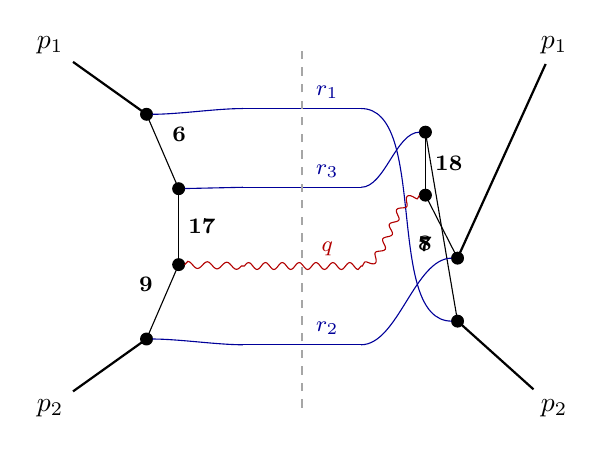
\begin{tikzpicture}
\begin{feynman}
\vertex (Lp1) at (-3.200,2.300) {$p_1$};
\vertex (Lp2) at (-3.200,-2.300) {$p_2$};
\vertex (Lcr1) at (-0.750,1.500);
\vertex (Lcr2) at (-0.750,-1.500);
\vertex (Lcr3) at (-0.750,0.500);
\vertex (Lcq) at (-0.750,-0.500);
\vertex[dot] (L6) at (-1.975,1.427) {};
\vertex[dot] (L17) at (-1.567,0.482) {};
\vertex[dot] (L9) at (-1.975,-1.427) {};
\vertex[dot] (Lroot) at (-1.567,-0.482) {};
\vertex (Rp1) at (3.200,2.300) {$p_1$};
\vertex (Rp2) at (3.200,-2.300) {$p_2$};
\vertex (Rcr1) at (0.750,1.500);
\vertex (Rcr2) at (0.750,-1.500);
\vertex (Rcr3) at (0.750,0.500);
\vertex (Rcq) at (0.750,-0.500);
\vertex[dot] (R7) at (1.975,-1.200) {};
\vertex[dot] (R18) at (1.567,1.200) {};
\vertex[dot] (R8) at (1.975,-0.400) {};
\vertex[dot] (Rroot) at (1.567,0.400) {};
\diagram* {
(L6) -- [plain, edge label={\footnotesize\bfseries 6}] (L17),
(L9) -- [plain, edge label={\footnotesize\bfseries 9}] (Lroot),
(L17) -- [plain, edge label={\footnotesize\bfseries 17}] (Lroot),
(Lp1) -- [plain, thick] (L6),
(Lp2) -- [plain, thick] (L9),
(Lcr1) -- [plain, blue!60!black, out=180, in=0, looseness=0.75] (L6),
(Lcr2) -- [plain, blue!60!black, out=180, in=0, looseness=0.75] (L9),
(Lcr3) -- [plain, blue!60!black] (L17),
(Lcq) -- [boson, red!70!black] (Lroot),
(R7) -- [plain, edge label={\footnotesize\bfseries 7}] (R18),
(R8) -- [plain, edge label={\footnotesize\bfseries 8}] (Rroot),
(R18) -- [plain, edge label={\footnotesize\bfseries 18}] (Rroot),
(Rp1) -- [plain, thick] (R8),
(Rp2) -- [plain, thick] (R7),
(Rcr1) -- [plain, blue!60!black, out=0, in=180, looseness=0.75] (R7),
(Rcr2) -- [plain, blue!60!black, out=0, in=180, looseness=0.75] (R8),
(Rcr3) -- [plain, blue!60!black, out=0, in=180, looseness=0.75] (R18),
(Rcq) -- [boson, red!70!black, out=0, in=180, looseness=0.75] (Rroot),
(Lcr1) -- [plain, blue!60!black] (Rcr1),
(Lcr2) -- [plain, blue!60!black] (Rcr2),
(Lcr3) -- [plain, blue!60!black] (Rcr3),
(Lcq) -- [boson, red!70!black] (Rcq),
};
\end{feynman}
\draw[dashed, gray!70] (0,-2.30) -- (0,2.30);
\node[font=\footnotesize, blue!60!black, above] at (0.32,1.50) {$r_1$};
\node[font=\footnotesize, blue!60!black, above] at (0.32,-1.50) {$r_2$};
\node[font=\footnotesize, blue!60!black, above] at (0.32,0.50) {$r_3$};
\node[font=\footnotesize, red!70!black, above] at (0.32,-0.50) {$q$};
\end{tikzpicture}}\\[2mm]\textbf{FAM[1]} (topo1)\\[2pt]{\footnotesize\begin{tabular}{@{}r@{\ \ }l@{\ \ }l@{}}\textbf{6} & $(p_1+r_1)^2$ & amplitude\\
\textbf{9} & $(p_2+r_2)^2$ & amplitude\\
\textbf{17} & $(p_1+r_1+r_3)^2$ & amplitude\\
\textbf{7} & $(p_2+r_1)^2$ & conjugate\\
\textbf{8} & $(p_1+r_2)^2$ & conjugate\\
\textbf{18} & $(p_2+r_1+r_3)^2$ & conjugate\\\end{tabular}}\\[2pt]{\scriptsize irreducible numerators: 27 = $(p_1+p_2+r_1+r_2)^2$}\end{minipage}\hfill%
\begin{minipage}[t]{0.48\textwidth}\centering\resizebox{0.9\linewidth}{!}{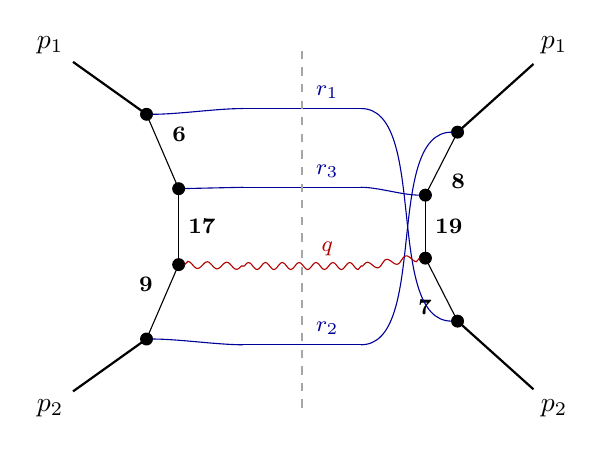
\begin{tikzpicture}
\begin{feynman}
\vertex (Lp1) at (-3.200,2.300) {$p_1$};
\vertex (Lp2) at (-3.200,-2.300) {$p_2$};
\vertex (Lcr1) at (-0.750,1.500);
\vertex (Lcr2) at (-0.750,-1.500);
\vertex (Lcr3) at (-0.750,0.500);
\vertex (Lcq) at (-0.750,-0.500);
\vertex[dot] (L6) at (-1.975,1.427) {};
\vertex[dot] (L17) at (-1.567,0.482) {};
\vertex[dot] (L9) at (-1.975,-1.427) {};
\vertex[dot] (Lroot) at (-1.567,-0.482) {};
\vertex (Rp1) at (3.200,2.300) {$p_1$};
\vertex (Rp2) at (3.200,-2.300) {$p_2$};
\vertex (Rcr1) at (0.750,1.500);
\vertex (Rcr2) at (0.750,-1.500);
\vertex (Rcr3) at (0.750,0.500);
\vertex (Rcq) at (0.750,-0.500);
\vertex[dot] (R7) at (1.975,-1.200) {};
\vertex[dot] (Rroot) at (1.567,-0.400) {};
\vertex[dot] (R8) at (1.975,1.200) {};
\vertex[dot] (R19) at (1.567,0.400) {};
\diagram* {
(L6) -- [plain, edge label={\footnotesize\bfseries 6}] (L17),
(L9) -- [plain, edge label={\footnotesize\bfseries 9}] (Lroot),
(L17) -- [plain, edge label={\footnotesize\bfseries 17}] (Lroot),
(Lp1) -- [plain, thick] (L6),
(Lp2) -- [plain, thick] (L9),
(Lcr1) -- [plain, blue!60!black, out=180, in=0, looseness=0.75] (L6),
(Lcr2) -- [plain, blue!60!black, out=180, in=0, looseness=0.75] (L9),
(Lcr3) -- [plain, blue!60!black] (L17),
(Lcq) -- [boson, red!70!black] (Lroot),
(R7) -- [plain, edge label={\footnotesize\bfseries 7}] (Rroot),
(R8) -- [plain, edge label={\footnotesize\bfseries 8}] (R19),
(R19) -- [plain, edge label={\footnotesize\bfseries 19}] (Rroot),
(Rp1) -- [plain, thick] (R8),
(Rp2) -- [plain, thick] (R7),
(Rcr1) -- [plain, blue!60!black, out=0, in=180, looseness=0.75] (R7),
(Rcr2) -- [plain, blue!60!black, out=0, in=180, looseness=0.75] (R8),
(Rcr3) -- [plain, blue!60!black, out=0, in=180, looseness=0.75] (R19),
(Rcq) -- [boson, red!70!black, out=0, in=180, looseness=0.75] (Rroot),
(Lcr1) -- [plain, blue!60!black] (Rcr1),
(Lcr2) -- [plain, blue!60!black] (Rcr2),
(Lcr3) -- [plain, blue!60!black] (Rcr3),
(Lcq) -- [boson, red!70!black] (Rcq),
};
\end{feynman}
\draw[dashed, gray!70] (0,-2.30) -- (0,2.30);
\node[font=\footnotesize, blue!60!black, above] at (0.32,1.50) {$r_1$};
\node[font=\footnotesize, blue!60!black, above] at (0.32,-1.50) {$r_2$};
\node[font=\footnotesize, blue!60!black, above] at (0.32,0.50) {$r_3$};
\node[font=\footnotesize, red!70!black, above] at (0.32,-0.50) {$q$};
\end{tikzpicture}}\\[2mm]\textbf{FAM[7]} (topo7)\\[2pt]{\footnotesize\begin{tabular}{@{}r@{\ \ }l@{\ \ }l@{}}\textbf{6} & $(p_1+r_1)^2$ & amplitude\\
\textbf{9} & $(p_2+r_2)^2$ & amplitude\\
\textbf{17} & $(p_1+r_1+r_3)^2$ & amplitude\\
\textbf{7} & $(p_2+r_1)^2$ & conjugate\\
\textbf{8} & $(p_1+r_2)^2$ & conjugate\\
\textbf{19} & $(p_1+r_2+r_3)^2$ & conjugate\\\end{tabular}}\\[2pt]{\scriptsize irreducible numerators: 13 = $(r_2+r_3)^2$}\end{minipage}

\bigskip

\begin{minipage}[t]{0.48\textwidth}\centering\resizebox{0.9\linewidth}{!}{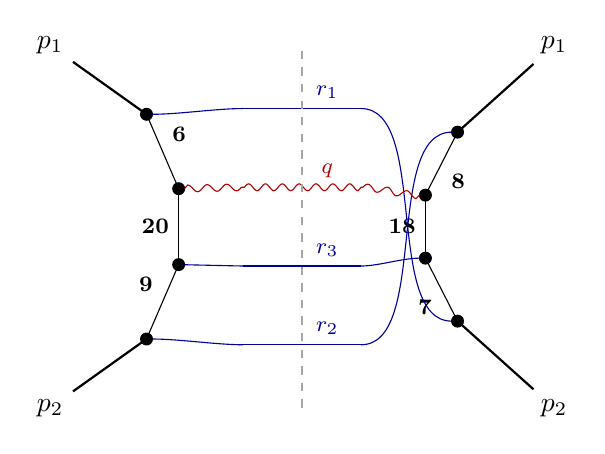
\begin{tikzpicture}
\begin{feynman}
\vertex (Lp1) at (-3.200,2.300) {$p_1$};
\vertex (Lp2) at (-3.200,-2.300) {$p_2$};
\vertex (Lcr1) at (-0.750,1.500);
\vertex (Lcr2) at (-0.750,-1.500);
\vertex (Lcr3) at (-0.750,-0.500);
\vertex (Lcq) at (-0.750,0.500);
\vertex[dot] (L6) at (-1.975,1.427) {};
\vertex[dot] (Lroot) at (-1.567,0.482) {};
\vertex[dot] (L9) at (-1.975,-1.427) {};
\vertex[dot] (L20) at (-1.567,-0.482) {};
\vertex (Rp1) at (3.200,2.300) {$p_1$};
\vertex (Rp2) at (3.200,-2.300) {$p_2$};
\vertex (Rcr1) at (0.750,1.500);
\vertex (Rcr2) at (0.750,-1.500);
\vertex (Rcr3) at (0.750,-0.500);
\vertex (Rcq) at (0.750,0.500);
\vertex[dot] (R7) at (1.975,-1.200) {};
\vertex[dot] (R18) at (1.567,-0.400) {};
\vertex[dot] (R8) at (1.975,1.200) {};
\vertex[dot] (Rroot) at (1.567,0.400) {};
\diagram* {
(L6) -- [plain, edge label={\footnotesize\bfseries 6}] (Lroot),
(L9) -- [plain, edge label={\footnotesize\bfseries 9}] (L20),
(L20) -- [plain, edge label={\footnotesize\bfseries 20}] (Lroot),
(Lp1) -- [plain, thick] (L6),
(Lp2) -- [plain, thick] (L9),
(Lcr1) -- [plain, blue!60!black, out=180, in=0, looseness=0.75] (L6),
(Lcr2) -- [plain, blue!60!black, out=180, in=0, looseness=0.75] (L9),
(Lcr3) -- [plain, blue!60!black] (L20),
(Lcq) -- [boson, red!70!black] (Lroot),
(R7) -- [plain, edge label={\footnotesize\bfseries 7}] (R18),
(R8) -- [plain, edge label={\footnotesize\bfseries 8}] (Rroot),
(R18) -- [plain, edge label={\footnotesize\bfseries 18}] (Rroot),
(Rp1) -- [plain, thick] (R8),
(Rp2) -- [plain, thick] (R7),
(Rcr1) -- [plain, blue!60!black, out=0, in=180, looseness=0.75] (R7),
(Rcr2) -- [plain, blue!60!black, out=0, in=180, looseness=0.75] (R8),
(Rcr3) -- [plain, blue!60!black, out=0, in=180, looseness=0.75] (R18),
(Rcq) -- [boson, red!70!black, out=0, in=180, looseness=0.75] (Rroot),
(Lcr1) -- [plain, blue!60!black] (Rcr1),
(Lcr2) -- [plain, blue!60!black] (Rcr2),
(Lcr3) -- [plain, blue!60!black] (Rcr3),
(Lcq) -- [boson, red!70!black] (Rcq),
};
\end{feynman}
\draw[dashed, gray!70] (0,-2.30) -- (0,2.30);
\node[font=\footnotesize, blue!60!black, above] at (0.32,1.50) {$r_1$};
\node[font=\footnotesize, blue!60!black, above] at (0.32,-1.50) {$r_2$};
\node[font=\footnotesize, blue!60!black, above] at (0.32,-0.50) {$r_3$};
\node[font=\footnotesize, red!70!black, above] at (0.32,0.50) {$q$};
\end{tikzpicture}}\\[2mm]\textbf{FAM[13]} (topo13)\\[2pt]{\footnotesize\begin{tabular}{@{}r@{\ \ }l@{\ \ }l@{}}\textbf{6} & $(p_1+r_1)^2$ & amplitude\\
\textbf{9} & $(p_2+r_2)^2$ & amplitude\\
\textbf{20} & $(p_2+r_2+r_3)^2$ & amplitude\\
\textbf{7} & $(p_2+r_1)^2$ & conjugate\\
\textbf{8} & $(p_1+r_2)^2$ & conjugate\\
\textbf{18} & $(p_2+r_1+r_3)^2$ & conjugate\\\end{tabular}}\\[2pt]{\scriptsize irreducible numerators: 13 = $(r_2+r_3)^2$}\end{minipage}\hfill%
\begin{minipage}[t]{0.48\textwidth}\centering\resizebox{0.9\linewidth}{!}{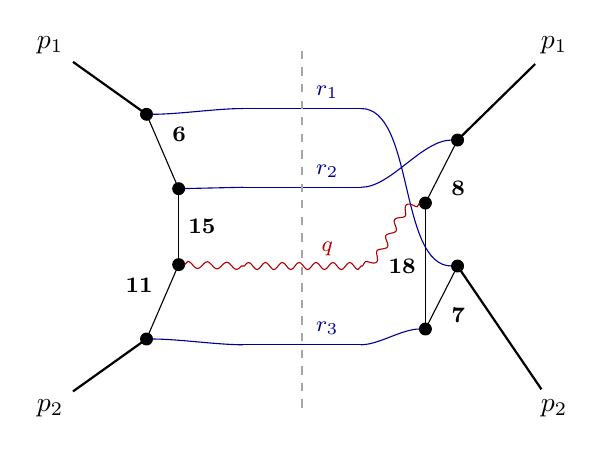
\begin{tikzpicture}
\begin{feynman}
\vertex (Lp1) at (-3.200,2.300) {$p_1$};
\vertex (Lp2) at (-3.200,-2.300) {$p_2$};
\vertex (Lcr1) at (-0.750,1.500);
\vertex (Lcr2) at (-0.750,0.500);
\vertex (Lcr3) at (-0.750,-1.500);
\vertex (Lcq) at (-0.750,-0.500);
\vertex[dot] (L6) at (-1.975,1.427) {};
\vertex[dot] (L15) at (-1.567,0.482) {};
\vertex[dot] (L11) at (-1.975,-1.427) {};
\vertex[dot] (Lroot) at (-1.567,-0.482) {};
\vertex (Rp1) at (3.200,2.300) {$p_1$};
\vertex (Rp2) at (3.200,-2.300) {$p_2$};
\vertex (Rcr1) at (0.750,1.500);
\vertex (Rcr2) at (0.750,0.500);
\vertex (Rcr3) at (0.750,-1.500);
\vertex (Rcq) at (0.750,-0.500);
\vertex[dot] (R7) at (1.975,-0.500) {};
\vertex[dot] (R18) at (1.567,-1.300) {};
\vertex[dot] (R8) at (1.975,1.100) {};
\vertex[dot] (Rroot) at (1.567,0.300) {};
\diagram* {
(L6) -- [plain, edge label={\footnotesize\bfseries 6}] (L15),
(L11) -- [plain, edge label={\footnotesize\bfseries 11}] (Lroot),
(L15) -- [plain, edge label={\footnotesize\bfseries 15}] (Lroot),
(Lp1) -- [plain, thick] (L6),
(Lp2) -- [plain, thick] (L11),
(Lcr1) -- [plain, blue!60!black, out=180, in=0, looseness=0.75] (L6),
(Lcr2) -- [plain, blue!60!black] (L15),
(Lcr3) -- [plain, blue!60!black, out=180, in=0, looseness=0.75] (L11),
(Lcq) -- [boson, red!70!black] (Lroot),
(R7) -- [plain, edge label={\footnotesize\bfseries 7}] (R18),
(R8) -- [plain, edge label={\footnotesize\bfseries 8}] (Rroot),
(R18) -- [plain, edge label={\footnotesize\bfseries 18}] (Rroot),
(Rp1) -- [plain, thick] (R8),
(Rp2) -- [plain, thick] (R7),
(Rcr1) -- [plain, blue!60!black, out=0, in=180, looseness=0.75] (R7),
(Rcr2) -- [plain, blue!60!black, out=0, in=180, looseness=0.75] (R8),
(Rcr3) -- [plain, blue!60!black, out=0, in=180, looseness=0.75] (R18),
(Rcq) -- [boson, red!70!black, out=0, in=180, looseness=0.75] (Rroot),
(Lcr1) -- [plain, blue!60!black] (Rcr1),
(Lcr2) -- [plain, blue!60!black] (Rcr2),
(Lcr3) -- [plain, blue!60!black] (Rcr3),
(Lcq) -- [boson, red!70!black] (Rcq),
};
\end{feynman}
\draw[dashed, gray!70] (0,-2.30) -- (0,2.30);
\node[font=\footnotesize, blue!60!black, above] at (0.32,1.50) {$r_1$};
\node[font=\footnotesize, blue!60!black, above] at (0.32,0.50) {$r_2$};
\node[font=\footnotesize, blue!60!black, above] at (0.32,-1.50) {$r_3$};
\node[font=\footnotesize, red!70!black, above] at (0.32,-0.50) {$q$};
\end{tikzpicture}}\\[2mm]\textbf{FAM[19]} (topo19)\\[2pt]{\footnotesize\begin{tabular}{@{}r@{\ \ }l@{\ \ }l@{}}\textbf{6} & $(p_1+r_1)^2$ & amplitude\\
\textbf{11} & $(p_2+r_3)^2$ & amplitude\\
\textbf{15} & $(p_1+r_1+r_2)^2$ & amplitude\\
\textbf{7} & $(p_2+r_1)^2$ & conjugate\\
\textbf{8} & $(p_1+r_2)^2$ & conjugate\\
\textbf{18} & $(p_2+r_1+r_3)^2$ & conjugate\\\end{tabular}}\\[2pt]{\scriptsize irreducible numerators: 27 = $(p_1+p_2+r_1+r_2)^2$}\end{minipage}

\bigskip

\begin{minipage}[t]{0.48\textwidth}\centering\resizebox{0.9\linewidth}{!}{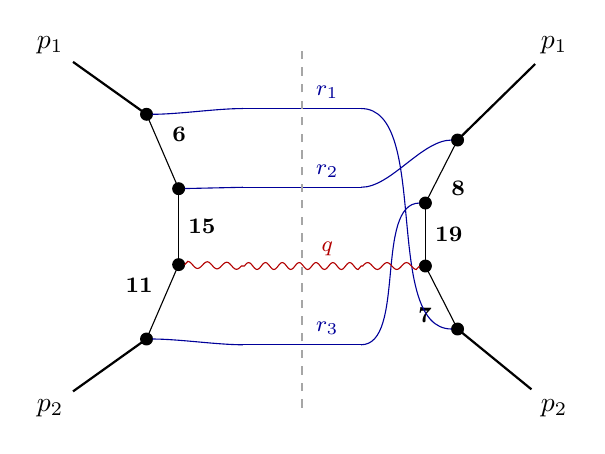
\begin{tikzpicture}
\begin{feynman}
\vertex (Lp1) at (-3.200,2.300) {$p_1$};
\vertex (Lp2) at (-3.200,-2.300) {$p_2$};
\vertex (Lcr1) at (-0.750,1.500);
\vertex (Lcr2) at (-0.750,0.500);
\vertex (Lcr3) at (-0.750,-1.500);
\vertex (Lcq) at (-0.750,-0.500);
\vertex[dot] (L6) at (-1.975,1.427) {};
\vertex[dot] (L15) at (-1.567,0.482) {};
\vertex[dot] (L11) at (-1.975,-1.427) {};
\vertex[dot] (Lroot) at (-1.567,-0.482) {};
\vertex (Rp1) at (3.200,2.300) {$p_1$};
\vertex (Rp2) at (3.200,-2.300) {$p_2$};
\vertex (Rcr1) at (0.750,1.500);
\vertex (Rcr2) at (0.750,0.500);
\vertex (Rcr3) at (0.750,-1.500);
\vertex (Rcq) at (0.750,-0.500);
\vertex[dot] (R7) at (1.975,-1.300) {};
\vertex[dot] (Rroot) at (1.567,-0.500) {};
\vertex[dot] (R8) at (1.975,1.100) {};
\vertex[dot] (R19) at (1.567,0.300) {};
\diagram* {
(L6) -- [plain, edge label={\footnotesize\bfseries 6}] (L15),
(L11) -- [plain, edge label={\footnotesize\bfseries 11}] (Lroot),
(L15) -- [plain, edge label={\footnotesize\bfseries 15}] (Lroot),
(Lp1) -- [plain, thick] (L6),
(Lp2) -- [plain, thick] (L11),
(Lcr1) -- [plain, blue!60!black, out=180, in=0, looseness=0.75] (L6),
(Lcr2) -- [plain, blue!60!black] (L15),
(Lcr3) -- [plain, blue!60!black, out=180, in=0, looseness=0.75] (L11),
(Lcq) -- [boson, red!70!black] (Lroot),
(R7) -- [plain, edge label={\footnotesize\bfseries 7}] (Rroot),
(R8) -- [plain, edge label={\footnotesize\bfseries 8}] (R19),
(R19) -- [plain, edge label={\footnotesize\bfseries 19}] (Rroot),
(Rp1) -- [plain, thick] (R8),
(Rp2) -- [plain, thick] (R7),
(Rcr1) -- [plain, blue!60!black, out=0, in=180, looseness=0.75] (R7),
(Rcr2) -- [plain, blue!60!black, out=0, in=180, looseness=0.75] (R8),
(Rcr3) -- [plain, blue!60!black, out=0, in=180, looseness=0.75] (R19),
(Rcq) -- [boson, red!70!black] (Rroot),
(Lcr1) -- [plain, blue!60!black] (Rcr1),
(Lcr2) -- [plain, blue!60!black] (Rcr2),
(Lcr3) -- [plain, blue!60!black] (Rcr3),
(Lcq) -- [boson, red!70!black] (Rcq),
};
\end{feynman}
\draw[dashed, gray!70] (0,-2.30) -- (0,2.30);
\node[font=\footnotesize, blue!60!black, above] at (0.32,1.50) {$r_1$};
\node[font=\footnotesize, blue!60!black, above] at (0.32,0.50) {$r_2$};
\node[font=\footnotesize, blue!60!black, above] at (0.32,-1.50) {$r_3$};
\node[font=\footnotesize, red!70!black, above] at (0.32,-0.50) {$q$};
\end{tikzpicture}}\\[2mm]\textbf{FAM[25]} (topo25)\\[2pt]{\footnotesize\begin{tabular}{@{}r@{\ \ }l@{\ \ }l@{}}\textbf{6} & $(p_1+r_1)^2$ & amplitude\\
\textbf{11} & $(p_2+r_3)^2$ & amplitude\\
\textbf{15} & $(p_1+r_1+r_2)^2$ & amplitude\\
\textbf{7} & $(p_2+r_1)^2$ & conjugate\\
\textbf{8} & $(p_1+r_2)^2$ & conjugate\\
\textbf{19} & $(p_1+r_2+r_3)^2$ & conjugate\\\end{tabular}}\\[2pt]{\scriptsize irreducible numerators: 22 = $(p_1+r_1+r_2+r_3)^2$}\end{minipage}\hfill%
\begin{minipage}[t]{0.48\textwidth}\centering\resizebox{0.9\linewidth}{!}{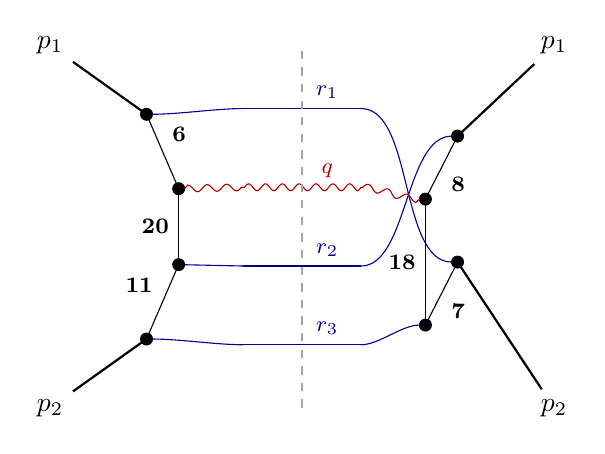
\begin{tikzpicture}
\begin{feynman}
\vertex (Lp1) at (-3.200,2.300) {$p_1$};
\vertex (Lp2) at (-3.200,-2.300) {$p_2$};
\vertex (Lcr1) at (-0.750,1.500);
\vertex (Lcr2) at (-0.750,-0.500);
\vertex (Lcr3) at (-0.750,-1.500);
\vertex (Lcq) at (-0.750,0.500);
\vertex[dot] (L6) at (-1.975,1.427) {};
\vertex[dot] (Lroot) at (-1.567,0.482) {};
\vertex[dot] (L11) at (-1.975,-1.427) {};
\vertex[dot] (L20) at (-1.567,-0.482) {};
\vertex (Rp1) at (3.200,2.300) {$p_1$};
\vertex (Rp2) at (3.200,-2.300) {$p_2$};
\vertex (Rcr1) at (0.750,1.500);
\vertex (Rcr2) at (0.750,-0.500);
\vertex (Rcr3) at (0.750,-1.500);
\vertex (Rcq) at (0.750,0.500);
\vertex[dot] (R7) at (1.975,-0.450) {};
\vertex[dot] (R18) at (1.567,-1.250) {};
\vertex[dot] (R8) at (1.975,1.150) {};
\vertex[dot] (Rroot) at (1.567,0.350) {};
\diagram* {
(L6) -- [plain, edge label={\footnotesize\bfseries 6}] (Lroot),
(L11) -- [plain, edge label={\footnotesize\bfseries 11}] (L20),
(L20) -- [plain, edge label={\footnotesize\bfseries 20}] (Lroot),
(Lp1) -- [plain, thick] (L6),
(Lp2) -- [plain, thick] (L11),
(Lcr1) -- [plain, blue!60!black, out=180, in=0, looseness=0.75] (L6),
(Lcr2) -- [plain, blue!60!black] (L20),
(Lcr3) -- [plain, blue!60!black, out=180, in=0, looseness=0.75] (L11),
(Lcq) -- [boson, red!70!black] (Lroot),
(R7) -- [plain, edge label={\footnotesize\bfseries 7}] (R18),
(R8) -- [plain, edge label={\footnotesize\bfseries 8}] (Rroot),
(R18) -- [plain, edge label={\footnotesize\bfseries 18}] (Rroot),
(Rp1) -- [plain, thick] (R8),
(Rp2) -- [plain, thick] (R7),
(Rcr1) -- [plain, blue!60!black, out=0, in=180, looseness=0.75] (R7),
(Rcr2) -- [plain, blue!60!black, out=0, in=180, looseness=0.75] (R8),
(Rcr3) -- [plain, blue!60!black, out=0, in=180, looseness=0.75] (R18),
(Rcq) -- [boson, red!70!black, out=0, in=180, looseness=0.75] (Rroot),
(Lcr1) -- [plain, blue!60!black] (Rcr1),
(Lcr2) -- [plain, blue!60!black] (Rcr2),
(Lcr3) -- [plain, blue!60!black] (Rcr3),
(Lcq) -- [boson, red!70!black] (Rcq),
};
\end{feynman}
\draw[dashed, gray!70] (0,-2.30) -- (0,2.30);
\node[font=\footnotesize, blue!60!black, above] at (0.32,1.50) {$r_1$};
\node[font=\footnotesize, blue!60!black, above] at (0.32,-0.50) {$r_2$};
\node[font=\footnotesize, blue!60!black, above] at (0.32,-1.50) {$r_3$};
\node[font=\footnotesize, red!70!black, above] at (0.32,0.50) {$q$};
\end{tikzpicture}}\\[2mm]\textbf{FAM[31]} (topo31)\\[2pt]{\footnotesize\begin{tabular}{@{}r@{\ \ }l@{\ \ }l@{}}\textbf{6} & $(p_1+r_1)^2$ & amplitude\\
\textbf{11} & $(p_2+r_3)^2$ & amplitude\\
\textbf{20} & $(p_2+r_2+r_3)^2$ & amplitude\\
\textbf{7} & $(p_2+r_1)^2$ & conjugate\\
\textbf{8} & $(p_1+r_2)^2$ & conjugate\\
\textbf{18} & $(p_2+r_1+r_3)^2$ & conjugate\\\end{tabular}}\\[2pt]{\scriptsize irreducible numerators: 23 = $(p_2+r_1+r_2+r_3)^2$}\end{minipage}

\bigskip

\begin{minipage}[t]{0.48\textwidth}\centering\resizebox{0.9\linewidth}{!}{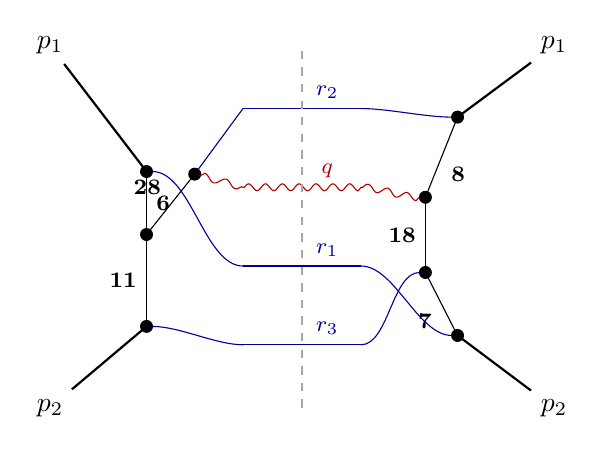
\begin{tikzpicture}
\begin{feynman}
\vertex (Lp1) at (-3.200,2.300) {$p_1$};
\vertex (Lp2) at (-3.200,-2.300) {$p_2$};
\vertex (Lcr1) at (-0.750,-0.500);
\vertex (Lcr2) at (-0.750,1.500);
\vertex (Lcr3) at (-0.750,-1.500);
\vertex (Lcq) at (-0.750,0.500);
\vertex[dot] (L6) at (-1.975,0.700) {};
\vertex[dot] (L28) at (-1.975,-0.100) {};
\vertex[dot] (L11) at (-1.975,-1.267) {};
\vertex[dot] (Lroot) at (-1.363,0.667) {};
\vertex (Rp1) at (3.200,2.300) {$p_1$};
\vertex (Rp2) at (3.200,-2.300) {$p_2$};
\vertex (Rcr1) at (0.750,-0.500);
\vertex (Rcr2) at (0.750,1.500);
\vertex (Rcr3) at (0.750,-1.500);
\vertex (Rcq) at (0.750,0.500);
\vertex[dot] (R7) at (1.975,-1.382) {};
\vertex[dot] (R18) at (1.567,-0.582) {};
\vertex[dot] (R8) at (1.975,1.391) {};
\vertex[dot] (Rroot) at (1.567,0.373) {};
\diagram* {
(L6) -- [plain, edge label={\footnotesize\bfseries 6}] (L28),
(L11) -- [plain, edge label={\footnotesize\bfseries 11}] (L28),
(L28) -- [plain, edge label={\footnotesize\bfseries 28}] (Lroot),
(Lp1) -- [plain, thick] (L6),
(Lp2) -- [plain, thick] (L11),
(Lcr1) -- [plain, blue!60!black, out=180, in=0, looseness=0.75] (L6),
(Lcr2) -- [plain, blue!60!black] (Lroot),
(Lcr3) -- [plain, blue!60!black, out=180, in=0, looseness=0.75] (L11),
(Lcq) -- [boson, red!70!black] (Lroot),
(R7) -- [plain, edge label={\footnotesize\bfseries 7}] (R18),
(R8) -- [plain, edge label={\footnotesize\bfseries 8}] (Rroot),
(R18) -- [plain, edge label={\footnotesize\bfseries 18}] (Rroot),
(Rp1) -- [plain, thick] (R8),
(Rp2) -- [plain, thick] (R7),
(Rcr1) -- [plain, blue!60!black, out=0, in=180, looseness=0.75] (R7),
(Rcr2) -- [plain, blue!60!black, out=0, in=180, looseness=0.75] (R8),
(Rcr3) -- [plain, blue!60!black, out=0, in=180, looseness=0.75] (R18),
(Rcq) -- [boson, red!70!black, out=0, in=180, looseness=0.75] (Rroot),
(Lcr1) -- [plain, blue!60!black] (Rcr1),
(Lcr2) -- [plain, blue!60!black] (Rcr2),
(Lcr3) -- [plain, blue!60!black] (Rcr3),
(Lcq) -- [boson, red!70!black] (Rcq),
};
\end{feynman}
\draw[dashed, gray!70] (0,-2.30) -- (0,2.30);
\node[font=\footnotesize, blue!60!black, above] at (0.32,-0.50) {$r_1$};
\node[font=\footnotesize, blue!60!black, above] at (0.32,1.50) {$r_2$};
\node[font=\footnotesize, blue!60!black, above] at (0.32,-1.50) {$r_3$};
\node[font=\footnotesize, red!70!black, above] at (0.32,0.50) {$q$};
\end{tikzpicture}}\\[2mm]\textbf{FAM[37]} (topo37)\\[2pt]{\footnotesize\begin{tabular}{@{}r@{\ \ }l@{\ \ }l@{}}\textbf{6} & $(p_1+r_1)^2$ & amplitude\\
\textbf{11} & $(p_2+r_3)^2$ & amplitude\\
\textbf{28} & $(p_1+p_2+r_1+r_3)^2$ & amplitude\\
\textbf{7} & $(p_2+r_1)^2$ & conjugate\\
\textbf{8} & $(p_1+r_2)^2$ & conjugate\\
\textbf{18} & $(p_2+r_1+r_3)^2$ & conjugate\\\end{tabular}}\\[2pt]{\scriptsize irreducible numerators: 27 = $(p_1+p_2+r_1+r_2)^2$}\end{minipage}\hfill%
\begin{minipage}[t]{0.48\textwidth}\centering\resizebox{0.9\linewidth}{!}{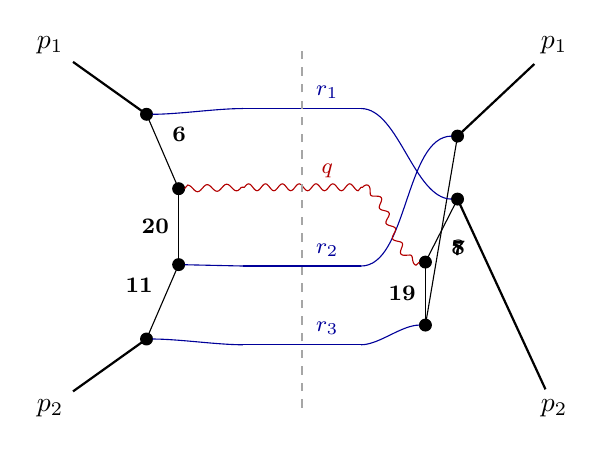
\begin{tikzpicture}
\begin{feynman}
\vertex (Lp1) at (-3.200,2.300) {$p_1$};
\vertex (Lp2) at (-3.200,-2.300) {$p_2$};
\vertex (Lcr1) at (-0.750,1.500);
\vertex (Lcr2) at (-0.750,-0.500);
\vertex (Lcr3) at (-0.750,-1.500);
\vertex (Lcq) at (-0.750,0.500);
\vertex[dot] (L6) at (-1.975,1.427) {};
\vertex[dot] (Lroot) at (-1.567,0.482) {};
\vertex[dot] (L11) at (-1.975,-1.427) {};
\vertex[dot] (L20) at (-1.567,-0.482) {};
\vertex (Rp1) at (3.200,2.300) {$p_1$};
\vertex (Rp2) at (3.200,-2.300) {$p_2$};
\vertex (Rcr1) at (0.750,1.500);
\vertex (Rcr2) at (0.750,-0.500);
\vertex (Rcr3) at (0.750,-1.500);
\vertex (Rcq) at (0.750,0.500);
\vertex[dot] (R7) at (1.975,0.350) {};
\vertex[dot] (Rroot) at (1.567,-0.450) {};
\vertex[dot] (R8) at (1.975,1.150) {};
\vertex[dot] (R19) at (1.567,-1.250) {};
\diagram* {
(L6) -- [plain, edge label={\footnotesize\bfseries 6}] (Lroot),
(L11) -- [plain, edge label={\footnotesize\bfseries 11}] (L20),
(L20) -- [plain, edge label={\footnotesize\bfseries 20}] (Lroot),
(Lp1) -- [plain, thick] (L6),
(Lp2) -- [plain, thick] (L11),
(Lcr1) -- [plain, blue!60!black, out=180, in=0, looseness=0.75] (L6),
(Lcr2) -- [plain, blue!60!black] (L20),
(Lcr3) -- [plain, blue!60!black, out=180, in=0, looseness=0.75] (L11),
(Lcq) -- [boson, red!70!black] (Lroot),
(R7) -- [plain, edge label={\footnotesize\bfseries 7}] (Rroot),
(R8) -- [plain, edge label={\footnotesize\bfseries 8}] (R19),
(R19) -- [plain, edge label={\footnotesize\bfseries 19}] (Rroot),
(Rp1) -- [plain, thick] (R8),
(Rp2) -- [plain, thick] (R7),
(Rcr1) -- [plain, blue!60!black, out=0, in=180, looseness=0.75] (R7),
(Rcr2) -- [plain, blue!60!black, out=0, in=180, looseness=0.75] (R8),
(Rcr3) -- [plain, blue!60!black, out=0, in=180, looseness=0.75] (R19),
(Rcq) -- [boson, red!70!black, out=0, in=180, looseness=0.75] (Rroot),
(Lcr1) -- [plain, blue!60!black] (Rcr1),
(Lcr2) -- [plain, blue!60!black] (Rcr2),
(Lcr3) -- [plain, blue!60!black] (Rcr3),
(Lcq) -- [boson, red!70!black] (Rcq),
};
\end{feynman}
\draw[dashed, gray!70] (0,-2.30) -- (0,2.30);
\node[font=\footnotesize, blue!60!black, above] at (0.32,1.50) {$r_1$};
\node[font=\footnotesize, blue!60!black, above] at (0.32,-0.50) {$r_2$};
\node[font=\footnotesize, blue!60!black, above] at (0.32,-1.50) {$r_3$};
\node[font=\footnotesize, red!70!black, above] at (0.32,0.50) {$q$};
\end{tikzpicture}}\\[2mm]\textbf{FAM[43]} (topo43)\\[2pt]{\footnotesize\begin{tabular}{@{}r@{\ \ }l@{\ \ }l@{}}\textbf{6} & $(p_1+r_1)^2$ & amplitude\\
\textbf{11} & $(p_2+r_3)^2$ & amplitude\\
\textbf{20} & $(p_2+r_2+r_3)^2$ & amplitude\\
\textbf{7} & $(p_2+r_1)^2$ & conjugate\\
\textbf{8} & $(p_1+r_2)^2$ & conjugate\\
\textbf{19} & $(p_1+r_2+r_3)^2$ & conjugate\\\end{tabular}}\\[2pt]{\scriptsize irreducible numerators: 27 = $(p_1+p_2+r_1+r_2)^2$}\end{minipage}

\bigskip

\begin{minipage}[t]{0.48\textwidth}\centering\resizebox{0.9\linewidth}{!}{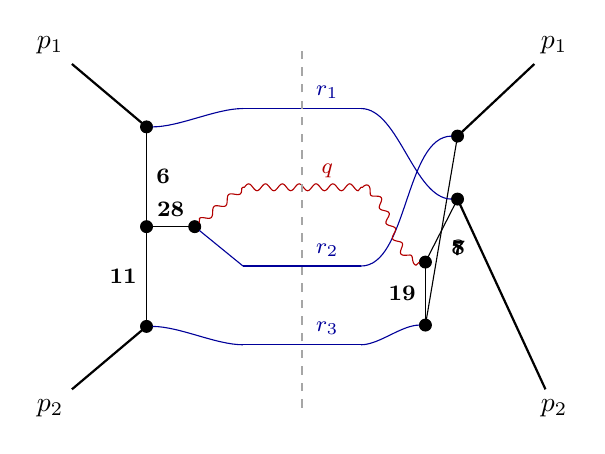
\begin{tikzpicture}
\begin{feynman}
\vertex (Lp1) at (-3.200,2.300) {$p_1$};
\vertex (Lp2) at (-3.200,-2.300) {$p_2$};
\vertex (Lcr1) at (-0.750,1.500);
\vertex (Lcr2) at (-0.750,-0.500);
\vertex (Lcr3) at (-0.750,-1.500);
\vertex (Lcq) at (-0.750,0.500);
\vertex[dot] (L6) at (-1.975,1.267) {};
\vertex[dot] (L28) at (-1.975,0.000) {};
\vertex[dot] (L11) at (-1.975,-1.267) {};
\vertex[dot] (Lroot) at (-1.363,0.000) {};
\vertex (Rp1) at (3.200,2.300) {$p_1$};
\vertex (Rp2) at (3.200,-2.300) {$p_2$};
\vertex (Rcr1) at (0.750,1.500);
\vertex (Rcr2) at (0.750,-0.500);
\vertex (Rcr3) at (0.750,-1.500);
\vertex (Rcq) at (0.750,0.500);
\vertex[dot] (R7) at (1.975,0.350) {};
\vertex[dot] (Rroot) at (1.567,-0.450) {};
\vertex[dot] (R8) at (1.975,1.150) {};
\vertex[dot] (R19) at (1.567,-1.250) {};
\diagram* {
(L6) -- [plain, edge label={\footnotesize\bfseries 6}] (L28),
(L11) -- [plain, edge label={\footnotesize\bfseries 11}] (L28),
(L28) -- [plain, edge label={\footnotesize\bfseries 28}] (Lroot),
(Lp1) -- [plain, thick] (L6),
(Lp2) -- [plain, thick] (L11),
(Lcr1) -- [plain, blue!60!black, out=180, in=0, looseness=0.75] (L6),
(Lcr2) -- [plain, blue!60!black] (Lroot),
(Lcr3) -- [plain, blue!60!black, out=180, in=0, looseness=0.75] (L11),
(Lcq) -- [boson, red!70!black] (Lroot),
(R7) -- [plain, edge label={\footnotesize\bfseries 7}] (Rroot),
(R8) -- [plain, edge label={\footnotesize\bfseries 8}] (R19),
(R19) -- [plain, edge label={\footnotesize\bfseries 19}] (Rroot),
(Rp1) -- [plain, thick] (R8),
(Rp2) -- [plain, thick] (R7),
(Rcr1) -- [plain, blue!60!black, out=0, in=180, looseness=0.75] (R7),
(Rcr2) -- [plain, blue!60!black, out=0, in=180, looseness=0.75] (R8),
(Rcr3) -- [plain, blue!60!black, out=0, in=180, looseness=0.75] (R19),
(Rcq) -- [boson, red!70!black, out=0, in=180, looseness=0.75] (Rroot),
(Lcr1) -- [plain, blue!60!black] (Rcr1),
(Lcr2) -- [plain, blue!60!black] (Rcr2),
(Lcr3) -- [plain, blue!60!black] (Rcr3),
(Lcq) -- [boson, red!70!black] (Rcq),
};
\end{feynman}
\draw[dashed, gray!70] (0,-2.30) -- (0,2.30);
\node[font=\footnotesize, blue!60!black, above] at (0.32,1.50) {$r_1$};
\node[font=\footnotesize, blue!60!black, above] at (0.32,-0.50) {$r_2$};
\node[font=\footnotesize, blue!60!black, above] at (0.32,-1.50) {$r_3$};
\node[font=\footnotesize, red!70!black, above] at (0.32,0.50) {$q$};
\end{tikzpicture}}\\[2mm]\textbf{FAM[49]} (topo49)\\[2pt]{\footnotesize\begin{tabular}{@{}r@{\ \ }l@{\ \ }l@{}}\textbf{6} & $(p_1+r_1)^2$ & amplitude\\
\textbf{11} & $(p_2+r_3)^2$ & amplitude\\
\textbf{28} & $(p_1+p_2+r_1+r_3)^2$ & amplitude\\
\textbf{7} & $(p_2+r_1)^2$ & conjugate\\
\textbf{8} & $(p_1+r_2)^2$ & conjugate\\
\textbf{19} & $(p_1+r_2+r_3)^2$ & conjugate\\\end{tabular}}\\[2pt]{\scriptsize irreducible numerators: 13 = $(r_2+r_3)^2$}\end{minipage}\hfill%
\begin{minipage}[t]{0.48\textwidth}\centering\resizebox{0.9\linewidth}{!}{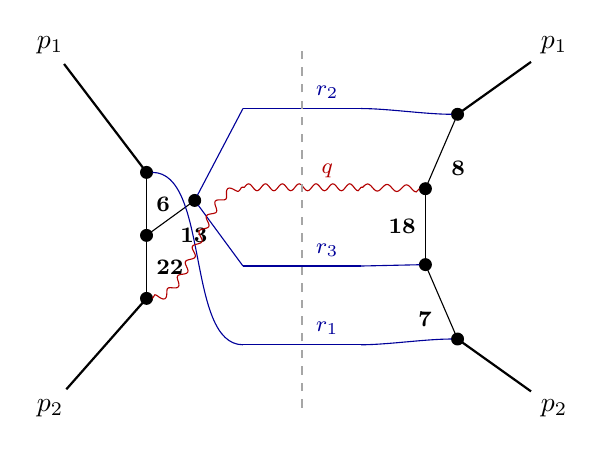
\begin{tikzpicture}
\begin{feynman}
\vertex (Lp1) at (-3.200,2.300) {$p_1$};
\vertex (Lp2) at (-3.200,-2.300) {$p_2$};
\vertex (Lcr1) at (-0.750,-1.500);
\vertex (Lcr2) at (-0.750,1.500);
\vertex (Lcr3) at (-0.750,-0.500);
\vertex (Lcq) at (-0.750,0.500);
\vertex[dot] (L6) at (-1.975,0.689) {};
\vertex[dot] (L22) at (-1.975,-0.111) {};
\vertex[dot] (L13) at (-1.363,0.333) {};
\vertex[dot] (Lroot) at (-1.975,-0.911) {};
\vertex (Rp1) at (3.200,2.300) {$p_1$};
\vertex (Rp2) at (3.200,-2.300) {$p_2$};
\vertex (Rcr1) at (0.750,-1.500);
\vertex (Rcr2) at (0.750,1.500);
\vertex (Rcr3) at (0.750,-0.500);
\vertex (Rcq) at (0.750,0.500);
\vertex[dot] (R7) at (1.975,-1.427) {};
\vertex[dot] (R18) at (1.567,-0.482) {};
\vertex[dot] (R8) at (1.975,1.427) {};
\vertex[dot] (Rroot) at (1.567,0.482) {};
\diagram* {
(L6) -- [plain, edge label={\footnotesize\bfseries 6}] (L22),
(L13) -- [plain, edge label={\footnotesize\bfseries 13}] (L22),
(L22) -- [plain, edge label={\footnotesize\bfseries 22}] (Lroot),
(Lp1) -- [plain, thick] (L6),
(Lp2) -- [plain, thick] (Lroot),
(Lcr1) -- [plain, blue!60!black, out=180, in=0, looseness=0.75] (L6),
(Lcr2) -- [plain, blue!60!black] (L13),
(Lcr3) -- [plain, blue!60!black] (L13),
(Lcq) -- [boson, red!70!black, out=180, in=0, looseness=0.75] (Lroot),
(R7) -- [plain, edge label={\footnotesize\bfseries 7}] (R18),
(R8) -- [plain, edge label={\footnotesize\bfseries 8}] (Rroot),
(R18) -- [plain, edge label={\footnotesize\bfseries 18}] (Rroot),
(Rp1) -- [plain, thick] (R8),
(Rp2) -- [plain, thick] (R7),
(Rcr1) -- [plain, blue!60!black, out=0, in=180, looseness=0.75] (R7),
(Rcr2) -- [plain, blue!60!black, out=0, in=180, looseness=0.75] (R8),
(Rcr3) -- [plain, blue!60!black] (R18),
(Rcq) -- [boson, red!70!black] (Rroot),
(Lcr1) -- [plain, blue!60!black] (Rcr1),
(Lcr2) -- [plain, blue!60!black] (Rcr2),
(Lcr3) -- [plain, blue!60!black] (Rcr3),
(Lcq) -- [boson, red!70!black] (Rcq),
};
\end{feynman}
\draw[dashed, gray!70] (0,-2.30) -- (0,2.30);
\node[font=\footnotesize, blue!60!black, above] at (0.32,-1.50) {$r_1$};
\node[font=\footnotesize, blue!60!black, above] at (0.32,1.50) {$r_2$};
\node[font=\footnotesize, blue!60!black, above] at (0.32,-0.50) {$r_3$};
\node[font=\footnotesize, red!70!black, above] at (0.32,0.50) {$q$};
\end{tikzpicture}}\\[2mm]\textbf{FAM[55]} (topo55)\\[2pt]{\footnotesize\begin{tabular}{@{}r@{\ \ }l@{\ \ }l@{}}\textbf{6} & $(p_1+r_1)^2$ & amplitude\\
\textbf{13} & $(r_2+r_3)^2$ & amplitude\\
\textbf{22} & $(p_1+r_1+r_2+r_3)^2$ & amplitude\\
\textbf{7} & $(p_2+r_1)^2$ & conjugate\\
\textbf{8} & $(p_1+r_2)^2$ & conjugate\\
\textbf{18} & $(p_2+r_1+r_3)^2$ & conjugate\\\end{tabular}}\\[2pt]{\scriptsize irreducible numerators: 14 = $(r_1+r_3)^2$}\end{minipage}

\bigskip

\begin{minipage}[t]{0.48\textwidth}\centering\resizebox{0.9\linewidth}{!}{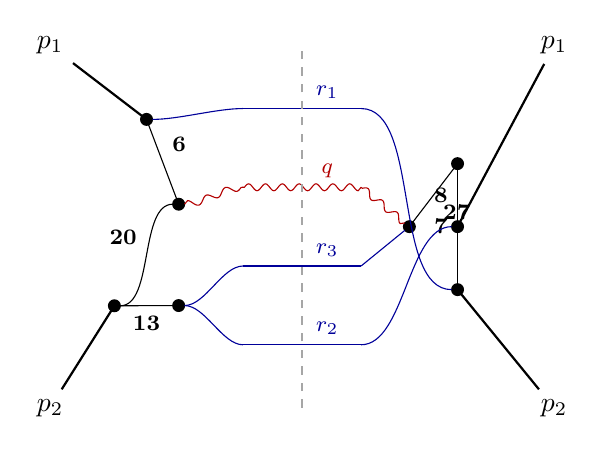
\begin{tikzpicture}
\begin{feynman}
\vertex (Lp1) at (-3.200,2.300) {$p_1$};
\vertex (Lp2) at (-3.200,-2.300) {$p_2$};
\vertex (Lcr1) at (-0.750,1.500);
\vertex (Lcr2) at (-0.750,-1.500);
\vertex (Lcr3) at (-0.750,-0.500);
\vertex (Lcq) at (-0.750,0.500);
\vertex[dot] (L6) at (-1.975,1.362) {};
\vertex[dot] (Lroot) at (-1.567,0.285) {};
\vertex[dot] (L13) at (-1.567,-1.002) {};
\vertex[dot] (L20) at (-2.383,-1.005) {};
\vertex (Rp1) at (3.200,2.300) {$p_1$};
\vertex (Rp2) at (3.200,-2.300) {$p_2$};
\vertex (Rcr1) at (0.750,1.500);
\vertex (Rcr2) at (0.750,-1.500);
\vertex (Rcr3) at (0.750,-0.500);
\vertex (Rcq) at (0.750,0.500);
\vertex[dot] (R7) at (1.975,-0.800) {};
\vertex[dot] (R27) at (1.975,0.800) {};
\vertex[dot] (R8) at (1.975,-0.000) {};
\vertex[dot] (Rroot) at (1.363,0.000) {};
\diagram* {
(L6) -- [plain, edge label={\footnotesize\bfseries 6}] (Lroot),
(L13) -- [plain, edge label={\footnotesize\bfseries 13}] (L20),
(L20) -- [plain, out=0, in=180, looseness=0.75, edge label={\footnotesize\bfseries 20}] (Lroot),
(Lp1) -- [plain, thick] (L6),
(Lp2) -- [plain, thick] (L20),
(Lcr1) -- [plain, blue!60!black, out=180, in=0, looseness=0.75] (L6),
(Lcr2) -- [plain, blue!60!black, out=180, in=0, looseness=0.75] (L13),
(Lcr3) -- [plain, blue!60!black, out=180, in=0, looseness=0.75] (L13),
(Lcq) -- [boson, red!70!black, out=180, in=0, looseness=0.75] (Lroot),
(R7) -- [plain, edge label={\footnotesize\bfseries 7}] (R27),
(R8) -- [plain, edge label={\footnotesize\bfseries 8}] (R27),
(R27) -- [plain, edge label={\footnotesize\bfseries 27}] (Rroot),
(Rp1) -- [plain, thick] (R8),
(Rp2) -- [plain, thick] (R7),
(Rcr1) -- [plain, blue!60!black, out=0, in=180, looseness=0.75] (R7),
(Rcr2) -- [plain, blue!60!black, out=0, in=180, looseness=0.75] (R8),
(Rcr3) -- [plain, blue!60!black] (Rroot),
(Rcq) -- [boson, red!70!black] (Rroot),
(Lcr1) -- [plain, blue!60!black] (Rcr1),
(Lcr2) -- [plain, blue!60!black] (Rcr2),
(Lcr3) -- [plain, blue!60!black] (Rcr3),
(Lcq) -- [boson, red!70!black] (Rcq),
};
\end{feynman}
\draw[dashed, gray!70] (0,-2.30) -- (0,2.30);
\node[font=\footnotesize, blue!60!black, above] at (0.32,1.50) {$r_1$};
\node[font=\footnotesize, blue!60!black, above] at (0.32,-1.50) {$r_2$};
\node[font=\footnotesize, blue!60!black, above] at (0.32,-0.50) {$r_3$};
\node[font=\footnotesize, red!70!black, above] at (0.32,0.50) {$q$};
\end{tikzpicture}}\\[2mm]\textbf{FAM[61]} (topo61)\\[2pt]{\footnotesize\begin{tabular}{@{}r@{\ \ }l@{\ \ }l@{}}\textbf{6} & $(p_1+r_1)^2$ & amplitude\\
\textbf{13} & $(r_2+r_3)^2$ & amplitude\\
\textbf{20} & $(p_2+r_2+r_3)^2$ & amplitude\\
\textbf{7} & $(p_2+r_1)^2$ & conjugate\\
\textbf{8} & $(p_1+r_2)^2$ & conjugate\\
\textbf{27} & $(p_1+p_2+r_1+r_2)^2$ & conjugate\\\end{tabular}}\\[2pt]{\scriptsize irreducible numerators: 25 = $(p_1+p_2+r_2)^2$}\end{minipage}\hfill%
\begin{minipage}[t]{0.48\textwidth}\centering\resizebox{0.9\linewidth}{!}{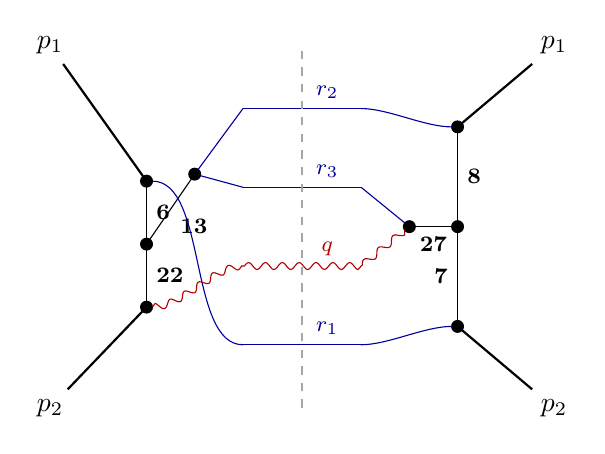
\begin{tikzpicture}
\begin{feynman}
\vertex (Lp1) at (-3.200,2.300) {$p_1$};
\vertex (Lp2) at (-3.200,-2.300) {$p_2$};
\vertex (Lcr1) at (-0.750,-1.500);
\vertex (Lcr2) at (-0.750,1.500);
\vertex (Lcr3) at (-0.750,0.500);
\vertex (Lcq) at (-0.750,-0.500);
\vertex[dot] (L6) at (-1.975,0.578) {};
\vertex[dot] (L22) at (-1.975,-0.222) {};
\vertex[dot] (L13) at (-1.363,0.667) {};
\vertex[dot] (Lroot) at (-1.975,-1.022) {};
\vertex (Rp1) at (3.200,2.300) {$p_1$};
\vertex (Rp2) at (3.200,-2.300) {$p_2$};
\vertex (Rcr1) at (0.750,-1.500);
\vertex (Rcr2) at (0.750,1.500);
\vertex (Rcr3) at (0.750,0.500);
\vertex (Rcq) at (0.750,-0.500);
\vertex[dot] (R7) at (1.975,-1.267) {};
\vertex[dot] (R27) at (1.975,0.000) {};
\vertex[dot] (R8) at (1.975,1.267) {};
\vertex[dot] (Rroot) at (1.363,0.000) {};
\diagram* {
(L6) -- [plain, edge label={\footnotesize\bfseries 6}] (L22),
(L13) -- [plain, edge label={\footnotesize\bfseries 13}] (L22),
(L22) -- [plain, edge label={\footnotesize\bfseries 22}] (Lroot),
(Lp1) -- [plain, thick] (L6),
(Lp2) -- [plain, thick] (Lroot),
(Lcr1) -- [plain, blue!60!black, out=180, in=0, looseness=0.75] (L6),
(Lcr2) -- [plain, blue!60!black] (L13),
(Lcr3) -- [plain, blue!60!black] (L13),
(Lcq) -- [boson, red!70!black, out=180, in=0, looseness=0.75] (Lroot),
(R7) -- [plain, edge label={\footnotesize\bfseries 7}] (R27),
(R8) -- [plain, edge label={\footnotesize\bfseries 8}] (R27),
(R27) -- [plain, edge label={\footnotesize\bfseries 27}] (Rroot),
(Rp1) -- [plain, thick] (R8),
(Rp2) -- [plain, thick] (R7),
(Rcr1) -- [plain, blue!60!black, out=0, in=180, looseness=0.75] (R7),
(Rcr2) -- [plain, blue!60!black, out=0, in=180, looseness=0.75] (R8),
(Rcr3) -- [plain, blue!60!black] (Rroot),
(Rcq) -- [boson, red!70!black] (Rroot),
(Lcr1) -- [plain, blue!60!black] (Rcr1),
(Lcr2) -- [plain, blue!60!black] (Rcr2),
(Lcr3) -- [plain, blue!60!black] (Rcr3),
(Lcq) -- [boson, red!70!black] (Rcq),
};
\end{feynman}
\draw[dashed, gray!70] (0,-2.30) -- (0,2.30);
\node[font=\footnotesize, blue!60!black, above] at (0.32,-1.50) {$r_1$};
\node[font=\footnotesize, blue!60!black, above] at (0.32,1.50) {$r_2$};
\node[font=\footnotesize, blue!60!black, above] at (0.32,0.50) {$r_3$};
\node[font=\footnotesize, red!70!black, above] at (0.32,-0.50) {$q$};
\end{tikzpicture}}\\[2mm]\textbf{FAM[67]} (topo67)\\[2pt]{\footnotesize\begin{tabular}{@{}r@{\ \ }l@{\ \ }l@{}}\textbf{6} & $(p_1+r_1)^2$ & amplitude\\
\textbf{13} & $(r_2+r_3)^2$ & amplitude\\
\textbf{22} & $(p_1+r_1+r_2+r_3)^2$ & amplitude\\
\textbf{7} & $(p_2+r_1)^2$ & conjugate\\
\textbf{8} & $(p_1+r_2)^2$ & conjugate\\
\textbf{27} & $(p_1+p_2+r_1+r_2)^2$ & conjugate\\\end{tabular}}\\[2pt]{\scriptsize irreducible numerators: 15 = $(p_1+r_1+r_2)^2$}\end{minipage}

\bigskip

\begin{minipage}[t]{0.48\textwidth}\centering\resizebox{0.9\linewidth}{!}{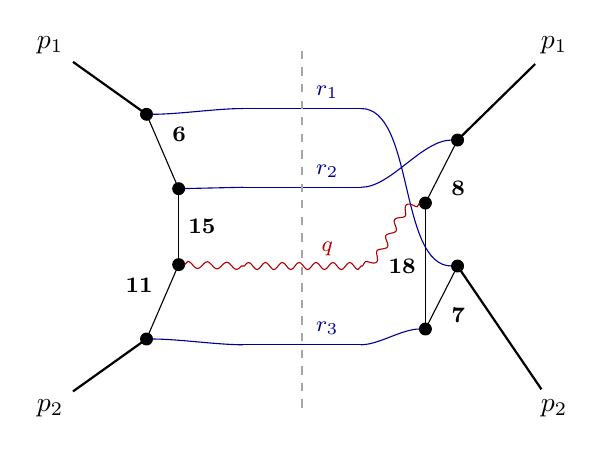
\begin{tikzpicture}
\begin{feynman}
\vertex (Lp1) at (-3.200,2.300) {$p_1$};
\vertex (Lp2) at (-3.200,-2.300) {$p_2$};
\vertex (Lcr1) at (-0.750,1.500);
\vertex (Lcr2) at (-0.750,0.500);
\vertex (Lcr3) at (-0.750,-1.500);
\vertex (Lcq) at (-0.750,-0.500);
\vertex[dot] (L6) at (-1.975,1.427) {};
\vertex[dot] (L15) at (-1.567,0.482) {};
\vertex[dot] (L11) at (-1.975,-1.427) {};
\vertex[dot] (Lroot) at (-1.567,-0.482) {};
\vertex (Rp1) at (3.200,2.300) {$p_1$};
\vertex (Rp2) at (3.200,-2.300) {$p_2$};
\vertex (Rcr1) at (0.750,1.500);
\vertex (Rcr2) at (0.750,0.500);
\vertex (Rcr3) at (0.750,-1.500);
\vertex (Rcq) at (0.750,-0.500);
\vertex[dot] (R7) at (1.975,-0.500) {};
\vertex[dot] (R18) at (1.567,-1.300) {};
\vertex[dot] (R8) at (1.975,1.100) {};
\vertex[dot] (Rroot) at (1.567,0.300) {};
\diagram* {
(L6) -- [plain, edge label={\footnotesize\bfseries 6}] (L15),
(L11) -- [plain, edge label={\footnotesize\bfseries 11}] (Lroot),
(L15) -- [plain, edge label={\footnotesize\bfseries 15}] (Lroot),
(Lp1) -- [plain, thick] (L6),
(Lp2) -- [plain, thick] (L11),
(Lcr1) -- [plain, blue!60!black, out=180, in=0, looseness=0.75] (L6),
(Lcr2) -- [plain, blue!60!black] (L15),
(Lcr3) -- [plain, blue!60!black, out=180, in=0, looseness=0.75] (L11),
(Lcq) -- [boson, red!70!black] (Lroot),
(R7) -- [plain, edge label={\footnotesize\bfseries 7}] (R18),
(R8) -- [plain, edge label={\footnotesize\bfseries 8}] (Rroot),
(R18) -- [plain, edge label={\footnotesize\bfseries 18}] (Rroot),
(Rp1) -- [plain, thick] (R8),
(Rp2) -- [plain, thick] (R7),
(Rcr1) -- [plain, blue!60!black, out=0, in=180, looseness=0.75] (R7),
(Rcr2) -- [plain, blue!60!black, out=0, in=180, looseness=0.75] (R8),
(Rcr3) -- [plain, blue!60!black, out=0, in=180, looseness=0.75] (R18),
(Rcq) -- [boson, red!70!black, out=0, in=180, looseness=0.75] (Rroot),
(Lcr1) -- [plain, blue!60!black] (Rcr1),
(Lcr2) -- [plain, blue!60!black] (Rcr2),
(Lcr3) -- [plain, blue!60!black] (Rcr3),
(Lcq) -- [boson, red!70!black] (Rcq),
};
\end{feynman}
\draw[dashed, gray!70] (0,-2.30) -- (0,2.30);
\node[font=\footnotesize, blue!60!black, above] at (0.32,1.50) {$r_1$};
\node[font=\footnotesize, blue!60!black, above] at (0.32,0.50) {$r_2$};
\node[font=\footnotesize, blue!60!black, above] at (0.32,-1.50) {$r_3$};
\node[font=\footnotesize, red!70!black, above] at (0.32,-0.50) {$q$};
\end{tikzpicture}}\\[2mm]\textbf{FAM[73]} (topo73)\\[2pt]{\footnotesize\begin{tabular}{@{}r@{\ \ }l@{\ \ }l@{}}\textbf{6} & $(p_1+r_1)^2$ & amplitude\\
\textbf{11} & $(p_2+r_3)^2$ & amplitude\\
\textbf{15} & $(p_1+r_1+r_2)^2$ & amplitude\\
\textbf{7} & $(p_2+r_1)^2$ & conjugate\\
\textbf{8} & $(p_1+r_2)^2$ & conjugate\\
\textbf{18} & $(p_2+r_1+r_3)^2$ & conjugate\\\end{tabular}}\\[2pt]{\scriptsize irreducible numerators: 22 = $(p_1+r_1+r_2+r_3)^2$}\end{minipage}\hfill%
\begin{minipage}[t]{0.48\textwidth}\centering\resizebox{0.9\linewidth}{!}{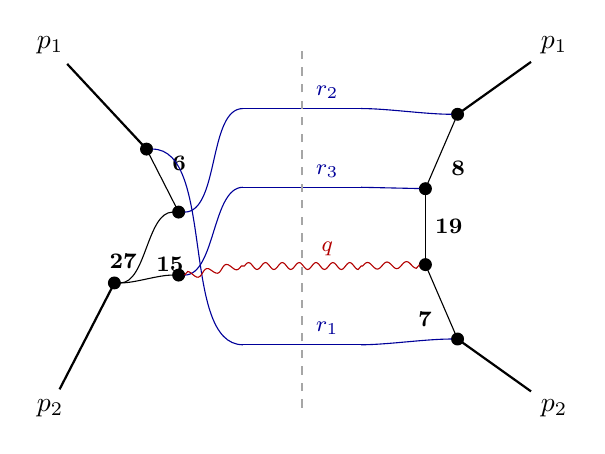
\begin{tikzpicture}
\begin{feynman}
\vertex (Lp1) at (-3.200,2.300) {$p_1$};
\vertex (Lp2) at (-3.200,-2.300) {$p_2$};
\vertex (Lcr1) at (-0.750,-1.500);
\vertex (Lcr2) at (-0.750,1.500);
\vertex (Lcr3) at (-0.750,0.500);
\vertex (Lcq) at (-0.750,-0.500);
\vertex[dot] (L6) at (-1.975,0.985) {};
\vertex[dot] (L15) at (-1.567,0.185) {};
\vertex[dot] (L27) at (-2.383,-0.715) {};
\vertex[dot] (Lroot) at (-1.567,-0.615) {};
\vertex (Rp1) at (3.200,2.300) {$p_1$};
\vertex (Rp2) at (3.200,-2.300) {$p_2$};
\vertex (Rcr1) at (0.750,-1.500);
\vertex (Rcr2) at (0.750,1.500);
\vertex (Rcr3) at (0.750,0.500);
\vertex (Rcq) at (0.750,-0.500);
\vertex[dot] (R7) at (1.975,-1.427) {};
\vertex[dot] (Rroot) at (1.567,-0.482) {};
\vertex[dot] (R8) at (1.975,1.427) {};
\vertex[dot] (R19) at (1.567,0.482) {};
\diagram* {
(L6) -- [plain, edge label={\footnotesize\bfseries 6}] (L15),
(L15) -- [plain, out=180, in=0, looseness=0.75, edge label={\footnotesize\bfseries 15}] (L27),
(L27) -- [plain, out=0, in=180, looseness=0.75, edge label={\footnotesize\bfseries 27}] (Lroot),
(Lp1) -- [plain, thick] (L6),
(Lp2) -- [plain, thick] (L27),
(Lcr1) -- [plain, blue!60!black, out=180, in=0, looseness=0.75] (L6),
(Lcr2) -- [plain, blue!60!black, out=180, in=0, looseness=0.75] (L15),
(Lcr3) -- [plain, blue!60!black, out=180, in=0, looseness=0.75] (Lroot),
(Lcq) -- [boson, red!70!black, out=180, in=0, looseness=0.75] (Lroot),
(R7) -- [plain, edge label={\footnotesize\bfseries 7}] (Rroot),
(R8) -- [plain, edge label={\footnotesize\bfseries 8}] (R19),
(R19) -- [plain, edge label={\footnotesize\bfseries 19}] (Rroot),
(Rp1) -- [plain, thick] (R8),
(Rp2) -- [plain, thick] (R7),
(Rcr1) -- [plain, blue!60!black, out=0, in=180, looseness=0.75] (R7),
(Rcr2) -- [plain, blue!60!black, out=0, in=180, looseness=0.75] (R8),
(Rcr3) -- [plain, blue!60!black] (R19),
(Rcq) -- [boson, red!70!black] (Rroot),
(Lcr1) -- [plain, blue!60!black] (Rcr1),
(Lcr2) -- [plain, blue!60!black] (Rcr2),
(Lcr3) -- [plain, blue!60!black] (Rcr3),
(Lcq) -- [boson, red!70!black] (Rcq),
};
\end{feynman}
\draw[dashed, gray!70] (0,-2.30) -- (0,2.30);
\node[font=\footnotesize, blue!60!black, above] at (0.32,-1.50) {$r_1$};
\node[font=\footnotesize, blue!60!black, above] at (0.32,1.50) {$r_2$};
\node[font=\footnotesize, blue!60!black, above] at (0.32,0.50) {$r_3$};
\node[font=\footnotesize, red!70!black, above] at (0.32,-0.50) {$q$};
\end{tikzpicture}}\\[2mm]\textbf{FAM[79]} (topo79)\\[2pt]{\footnotesize\begin{tabular}{@{}r@{\ \ }l@{\ \ }l@{}}\textbf{6} & $(p_1+r_1)^2$ & amplitude\\
\textbf{15} & $(p_1+r_1+r_2)^2$ & amplitude\\
\textbf{27} & $(p_1+p_2+r_1+r_2)^2$ & amplitude\\
\textbf{7} & $(p_2+r_1)^2$ & conjugate\\
\textbf{8} & $(p_1+r_2)^2$ & conjugate\\
\textbf{19} & $(p_1+r_2+r_3)^2$ & conjugate\\\end{tabular}}\\[2pt]{\scriptsize irreducible numerators: 13 = $(r_2+r_3)^2$}\end{minipage}

\bigskip

\begin{minipage}[t]{0.48\textwidth}\centering\resizebox{0.9\linewidth}{!}{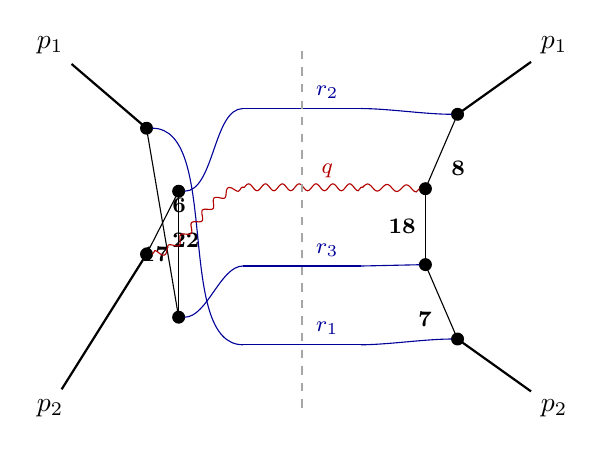
\begin{tikzpicture}
\begin{feynman}
\vertex (Lp1) at (-3.200,2.300) {$p_1$};
\vertex (Lp2) at (-3.200,-2.300) {$p_2$};
\vertex (Lcr1) at (-0.750,-1.500);
\vertex (Lcr2) at (-0.750,1.500);
\vertex (Lcr3) at (-0.750,-0.500);
\vertex (Lcq) at (-0.750,0.500);
\vertex[dot] (L6) at (-1.975,1.250) {};
\vertex[dot] (L17) at (-1.567,-1.150) {};
\vertex[dot] (L22) at (-1.567,0.450) {};
\vertex[dot] (Lroot) at (-1.975,-0.350) {};
\vertex (Rp1) at (3.200,2.300) {$p_1$};
\vertex (Rp2) at (3.200,-2.300) {$p_2$};
\vertex (Rcr1) at (0.750,-1.500);
\vertex (Rcr2) at (0.750,1.500);
\vertex (Rcr3) at (0.750,-0.500);
\vertex (Rcq) at (0.750,0.500);
\vertex[dot] (R7) at (1.975,-1.427) {};
\vertex[dot] (R18) at (1.567,-0.482) {};
\vertex[dot] (R8) at (1.975,1.427) {};
\vertex[dot] (Rroot) at (1.567,0.482) {};
\diagram* {
(L6) -- [plain, edge label={\footnotesize\bfseries 6}] (L17),
(L17) -- [plain, edge label={\footnotesize\bfseries 17}] (L22),
(L22) -- [plain, edge label={\footnotesize\bfseries 22}] (Lroot),
(Lp1) -- [plain, thick] (L6),
(Lp2) -- [plain, thick] (Lroot),
(Lcr1) -- [plain, blue!60!black, out=180, in=0, looseness=0.75] (L6),
(Lcr2) -- [plain, blue!60!black, out=180, in=0, looseness=0.75] (L22),
(Lcr3) -- [plain, blue!60!black, out=180, in=0, looseness=0.75] (L17),
(Lcq) -- [boson, red!70!black, out=180, in=0, looseness=0.75] (Lroot),
(R7) -- [plain, edge label={\footnotesize\bfseries 7}] (R18),
(R8) -- [plain, edge label={\footnotesize\bfseries 8}] (Rroot),
(R18) -- [plain, edge label={\footnotesize\bfseries 18}] (Rroot),
(Rp1) -- [plain, thick] (R8),
(Rp2) -- [plain, thick] (R7),
(Rcr1) -- [plain, blue!60!black, out=0, in=180, looseness=0.75] (R7),
(Rcr2) -- [plain, blue!60!black, out=0, in=180, looseness=0.75] (R8),
(Rcr3) -- [plain, blue!60!black] (R18),
(Rcq) -- [boson, red!70!black] (Rroot),
(Lcr1) -- [plain, blue!60!black] (Rcr1),
(Lcr2) -- [plain, blue!60!black] (Rcr2),
(Lcr3) -- [plain, blue!60!black] (Rcr3),
(Lcq) -- [boson, red!70!black] (Rcq),
};
\end{feynman}
\draw[dashed, gray!70] (0,-2.30) -- (0,2.30);
\node[font=\footnotesize, blue!60!black, above] at (0.32,-1.50) {$r_1$};
\node[font=\footnotesize, blue!60!black, above] at (0.32,1.50) {$r_2$};
\node[font=\footnotesize, blue!60!black, above] at (0.32,-0.50) {$r_3$};
\node[font=\footnotesize, red!70!black, above] at (0.32,0.50) {$q$};
\end{tikzpicture}}\\[2mm]\textbf{FAM[85]} (topo85)\\[2pt]{\footnotesize\begin{tabular}{@{}r@{\ \ }l@{\ \ }l@{}}\textbf{6} & $(p_1+r_1)^2$ & amplitude\\
\textbf{17} & $(p_1+r_1+r_3)^2$ & amplitude\\
\textbf{22} & $(p_1+r_1+r_2+r_3)^2$ & amplitude\\
\textbf{7} & $(p_2+r_1)^2$ & conjugate\\
\textbf{8} & $(p_1+r_2)^2$ & conjugate\\
\textbf{18} & $(p_2+r_1+r_3)^2$ & conjugate\\\end{tabular}}\\[2pt]{\scriptsize irreducible numerators: 19 = $(p_1+r_2+r_3)^2$}\end{minipage}\hfill%
\begin{minipage}[t]{0.48\textwidth}\centering\resizebox{0.9\linewidth}{!}{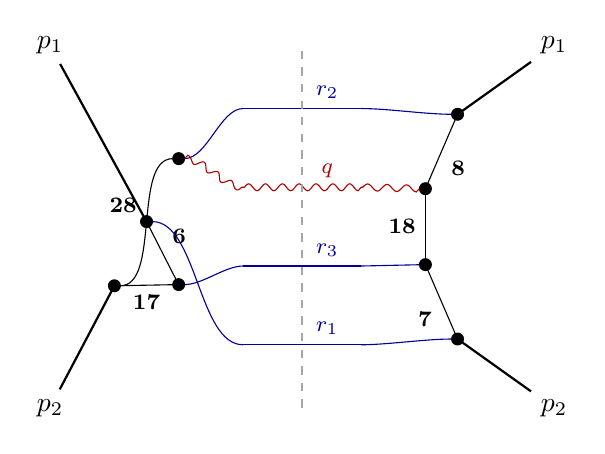
\begin{tikzpicture}
\begin{feynman}
\vertex (Lp1) at (-3.200,2.300) {$p_1$};
\vertex (Lp2) at (-3.200,-2.300) {$p_2$};
\vertex (Lcr1) at (-0.750,-1.500);
\vertex (Lcr2) at (-0.750,1.500);
\vertex (Lcr3) at (-0.750,-0.500);
\vertex (Lcq) at (-0.750,0.500);
\vertex[dot] (L6) at (-1.975,0.064) {};
\vertex[dot] (L17) at (-1.567,-0.736) {};
\vertex[dot] (L28) at (-2.383,-0.751) {};
\vertex[dot] (Lroot) at (-1.567,0.864) {};
\vertex (Rp1) at (3.200,2.300) {$p_1$};
\vertex (Rp2) at (3.200,-2.300) {$p_2$};
\vertex (Rcr1) at (0.750,-1.500);
\vertex (Rcr2) at (0.750,1.500);
\vertex (Rcr3) at (0.750,-0.500);
\vertex (Rcq) at (0.750,0.500);
\vertex[dot] (R7) at (1.975,-1.427) {};
\vertex[dot] (R18) at (1.567,-0.482) {};
\vertex[dot] (R8) at (1.975,1.427) {};
\vertex[dot] (Rroot) at (1.567,0.482) {};
\diagram* {
(L6) -- [plain, edge label={\footnotesize\bfseries 6}] (L17),
(L17) -- [plain, edge label={\footnotesize\bfseries 17}] (L28),
(L28) -- [plain, out=0, in=180, looseness=0.75, edge label={\footnotesize\bfseries 28}] (Lroot),
(Lp1) -- [plain, thick] (L6),
(Lp2) -- [plain, thick] (L28),
(Lcr1) -- [plain, blue!60!black, out=180, in=0, looseness=0.75] (L6),
(Lcr2) -- [plain, blue!60!black, out=180, in=0, looseness=0.75] (Lroot),
(Lcr3) -- [plain, blue!60!black, out=180, in=0, looseness=0.75] (L17),
(Lcq) -- [boson, red!70!black, out=180, in=0, looseness=0.75] (Lroot),
(R7) -- [plain, edge label={\footnotesize\bfseries 7}] (R18),
(R8) -- [plain, edge label={\footnotesize\bfseries 8}] (Rroot),
(R18) -- [plain, edge label={\footnotesize\bfseries 18}] (Rroot),
(Rp1) -- [plain, thick] (R8),
(Rp2) -- [plain, thick] (R7),
(Rcr1) -- [plain, blue!60!black, out=0, in=180, looseness=0.75] (R7),
(Rcr2) -- [plain, blue!60!black, out=0, in=180, looseness=0.75] (R8),
(Rcr3) -- [plain, blue!60!black] (R18),
(Rcq) -- [boson, red!70!black] (Rroot),
(Lcr1) -- [plain, blue!60!black] (Rcr1),
(Lcr2) -- [plain, blue!60!black] (Rcr2),
(Lcr3) -- [plain, blue!60!black] (Rcr3),
(Lcq) -- [boson, red!70!black] (Rcq),
};
\end{feynman}
\draw[dashed, gray!70] (0,-2.30) -- (0,2.30);
\node[font=\footnotesize, blue!60!black, above] at (0.32,-1.50) {$r_1$};
\node[font=\footnotesize, blue!60!black, above] at (0.32,1.50) {$r_2$};
\node[font=\footnotesize, blue!60!black, above] at (0.32,-0.50) {$r_3$};
\node[font=\footnotesize, red!70!black, above] at (0.32,0.50) {$q$};
\end{tikzpicture}}\\[2mm]\textbf{FAM[91]} (topo91)\\[2pt]{\footnotesize\begin{tabular}{@{}r@{\ \ }l@{\ \ }l@{}}\textbf{6} & $(p_1+r_1)^2$ & amplitude\\
\textbf{17} & $(p_1+r_1+r_3)^2$ & amplitude\\
\textbf{28} & $(p_1+p_2+r_1+r_3)^2$ & amplitude\\
\textbf{7} & $(p_2+r_1)^2$ & conjugate\\
\textbf{8} & $(p_1+r_2)^2$ & conjugate\\
\textbf{18} & $(p_2+r_1+r_3)^2$ & conjugate\\\end{tabular}}\\[2pt]{\scriptsize irreducible numerators: 19 = $(p_1+r_2+r_3)^2$}\end{minipage}

\bigskip

\begin{minipage}[t]{0.48\textwidth}\centering\resizebox{0.9\linewidth}{!}{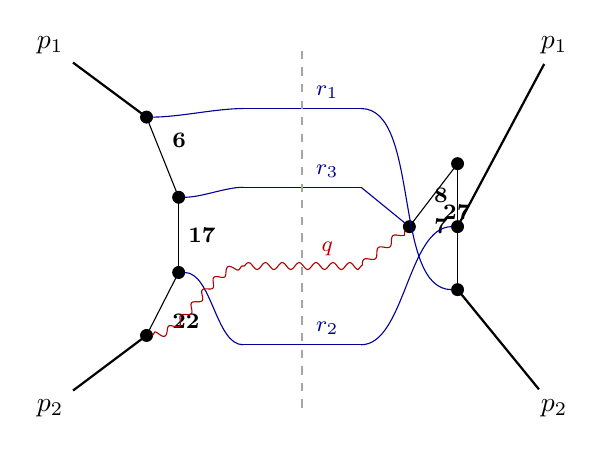
\begin{tikzpicture}
\begin{feynman}
\vertex (Lp1) at (-3.200,2.300) {$p_1$};
\vertex (Lp2) at (-3.200,-2.300) {$p_2$};
\vertex (Lcr1) at (-0.750,1.500);
\vertex (Lcr2) at (-0.750,-1.500);
\vertex (Lcr3) at (-0.750,0.500);
\vertex (Lcq) at (-0.750,-0.500);
\vertex[dot] (L6) at (-1.975,1.391) {};
\vertex[dot] (L17) at (-1.567,0.373) {};
\vertex[dot] (L22) at (-1.567,-0.582) {};
\vertex[dot] (Lroot) at (-1.975,-1.382) {};
\vertex (Rp1) at (3.200,2.300) {$p_1$};
\vertex (Rp2) at (3.200,-2.300) {$p_2$};
\vertex (Rcr1) at (0.750,1.500);
\vertex (Rcr2) at (0.750,-1.500);
\vertex (Rcr3) at (0.750,0.500);
\vertex (Rcq) at (0.750,-0.500);
\vertex[dot] (R7) at (1.975,-0.800) {};
\vertex[dot] (R27) at (1.975,0.800) {};
\vertex[dot] (R8) at (1.975,-0.000) {};
\vertex[dot] (Rroot) at (1.363,0.000) {};
\diagram* {
(L6) -- [plain, edge label={\footnotesize\bfseries 6}] (L17),
(L17) -- [plain, edge label={\footnotesize\bfseries 17}] (L22),
(L22) -- [plain, edge label={\footnotesize\bfseries 22}] (Lroot),
(Lp1) -- [plain, thick] (L6),
(Lp2) -- [plain, thick] (Lroot),
(Lcr1) -- [plain, blue!60!black, out=180, in=0, looseness=0.75] (L6),
(Lcr2) -- [plain, blue!60!black, out=180, in=0, looseness=0.75] (L22),
(Lcr3) -- [plain, blue!60!black, out=180, in=0, looseness=0.75] (L17),
(Lcq) -- [boson, red!70!black, out=180, in=0, looseness=0.75] (Lroot),
(R7) -- [plain, edge label={\footnotesize\bfseries 7}] (R27),
(R8) -- [plain, edge label={\footnotesize\bfseries 8}] (R27),
(R27) -- [plain, edge label={\footnotesize\bfseries 27}] (Rroot),
(Rp1) -- [plain, thick] (R8),
(Rp2) -- [plain, thick] (R7),
(Rcr1) -- [plain, blue!60!black, out=0, in=180, looseness=0.75] (R7),
(Rcr2) -- [plain, blue!60!black, out=0, in=180, looseness=0.75] (R8),
(Rcr3) -- [plain, blue!60!black] (Rroot),
(Rcq) -- [boson, red!70!black] (Rroot),
(Lcr1) -- [plain, blue!60!black] (Rcr1),
(Lcr2) -- [plain, blue!60!black] (Rcr2),
(Lcr3) -- [plain, blue!60!black] (Rcr3),
(Lcq) -- [boson, red!70!black] (Rcq),
};
\end{feynman}
\draw[dashed, gray!70] (0,-2.30) -- (0,2.30);
\node[font=\footnotesize, blue!60!black, above] at (0.32,1.50) {$r_1$};
\node[font=\footnotesize, blue!60!black, above] at (0.32,-1.50) {$r_2$};
\node[font=\footnotesize, blue!60!black, above] at (0.32,0.50) {$r_3$};
\node[font=\footnotesize, red!70!black, above] at (0.32,-0.50) {$q$};
\end{tikzpicture}}\\[2mm]\textbf{FAM[97]} (topo97)\\[2pt]{\footnotesize\begin{tabular}{@{}r@{\ \ }l@{\ \ }l@{}}\textbf{6} & $(p_1+r_1)^2$ & amplitude\\
\textbf{17} & $(p_1+r_1+r_3)^2$ & amplitude\\
\textbf{22} & $(p_1+r_1+r_2+r_3)^2$ & amplitude\\
\textbf{7} & $(p_2+r_1)^2$ & conjugate\\
\textbf{8} & $(p_1+r_2)^2$ & conjugate\\
\textbf{27} & $(p_1+p_2+r_1+r_2)^2$ & conjugate\\\end{tabular}}\\[2pt]{\scriptsize irreducible numerators: 25 = $(p_1+p_2+r_2)^2$}\end{minipage}\hfill%
\begin{minipage}[t]{0.48\textwidth}\centering\resizebox{0.9\linewidth}{!}{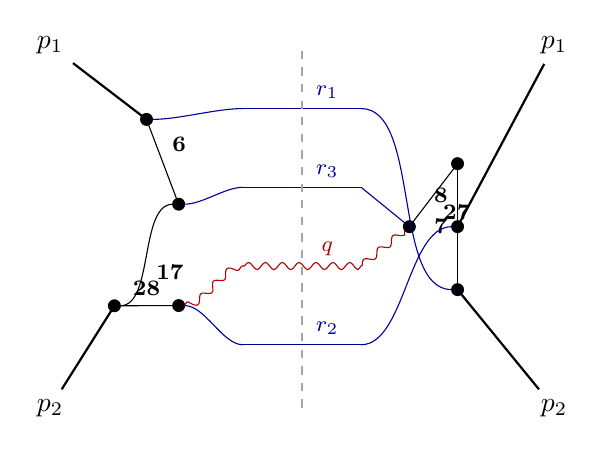
\begin{tikzpicture}
\begin{feynman}
\vertex (Lp1) at (-3.200,2.300) {$p_1$};
\vertex (Lp2) at (-3.200,-2.300) {$p_2$};
\vertex (Lcr1) at (-0.750,1.500);
\vertex (Lcr2) at (-0.750,-1.500);
\vertex (Lcr3) at (-0.750,0.500);
\vertex (Lcq) at (-0.750,-0.500);
\vertex[dot] (L6) at (-1.975,1.362) {};
\vertex[dot] (L17) at (-1.567,0.285) {};
\vertex[dot] (L28) at (-2.383,-1.005) {};
\vertex[dot] (Lroot) at (-1.567,-1.002) {};
\vertex (Rp1) at (3.200,2.300) {$p_1$};
\vertex (Rp2) at (3.200,-2.300) {$p_2$};
\vertex (Rcr1) at (0.750,1.500);
\vertex (Rcr2) at (0.750,-1.500);
\vertex (Rcr3) at (0.750,0.500);
\vertex (Rcq) at (0.750,-0.500);
\vertex[dot] (R7) at (1.975,-0.800) {};
\vertex[dot] (R27) at (1.975,0.800) {};
\vertex[dot] (R8) at (1.975,-0.000) {};
\vertex[dot] (Rroot) at (1.363,0.000) {};
\diagram* {
(L6) -- [plain, edge label={\footnotesize\bfseries 6}] (L17),
(L17) -- [plain, out=180, in=0, looseness=0.75, edge label={\footnotesize\bfseries 17}] (L28),
(L28) -- [plain, edge label={\footnotesize\bfseries 28}] (Lroot),
(Lp1) -- [plain, thick] (L6),
(Lp2) -- [plain, thick] (L28),
(Lcr1) -- [plain, blue!60!black, out=180, in=0, looseness=0.75] (L6),
(Lcr2) -- [plain, blue!60!black, out=180, in=0, looseness=0.75] (Lroot),
(Lcr3) -- [plain, blue!60!black, out=180, in=0, looseness=0.75] (L17),
(Lcq) -- [boson, red!70!black, out=180, in=0, looseness=0.75] (Lroot),
(R7) -- [plain, edge label={\footnotesize\bfseries 7}] (R27),
(R8) -- [plain, edge label={\footnotesize\bfseries 8}] (R27),
(R27) -- [plain, edge label={\footnotesize\bfseries 27}] (Rroot),
(Rp1) -- [plain, thick] (R8),
(Rp2) -- [plain, thick] (R7),
(Rcr1) -- [plain, blue!60!black, out=0, in=180, looseness=0.75] (R7),
(Rcr2) -- [plain, blue!60!black, out=0, in=180, looseness=0.75] (R8),
(Rcr3) -- [plain, blue!60!black] (Rroot),
(Rcq) -- [boson, red!70!black] (Rroot),
(Lcr1) -- [plain, blue!60!black] (Rcr1),
(Lcr2) -- [plain, blue!60!black] (Rcr2),
(Lcr3) -- [plain, blue!60!black] (Rcr3),
(Lcq) -- [boson, red!70!black] (Rcq),
};
\end{feynman}
\draw[dashed, gray!70] (0,-2.30) -- (0,2.30);
\node[font=\footnotesize, blue!60!black, above] at (0.32,1.50) {$r_1$};
\node[font=\footnotesize, blue!60!black, above] at (0.32,-1.50) {$r_2$};
\node[font=\footnotesize, blue!60!black, above] at (0.32,0.50) {$r_3$};
\node[font=\footnotesize, red!70!black, above] at (0.32,-0.50) {$q$};
\end{tikzpicture}}\\[2mm]\textbf{FAM[103]} (topo103)\\[2pt]{\footnotesize\begin{tabular}{@{}r@{\ \ }l@{\ \ }l@{}}\textbf{6} & $(p_1+r_1)^2$ & amplitude\\
\textbf{17} & $(p_1+r_1+r_3)^2$ & amplitude\\
\textbf{28} & $(p_1+p_2+r_1+r_3)^2$ & amplitude\\
\textbf{7} & $(p_2+r_1)^2$ & conjugate\\
\textbf{8} & $(p_1+r_2)^2$ & conjugate\\
\textbf{27} & $(p_1+p_2+r_1+r_2)^2$ & conjugate\\\end{tabular}}\\[2pt]{\scriptsize irreducible numerators: 14 = $(r_1+r_3)^2$}\end{minipage}

\bigskip

\begin{minipage}[t]{0.48\textwidth}\centering\resizebox{0.9\linewidth}{!}{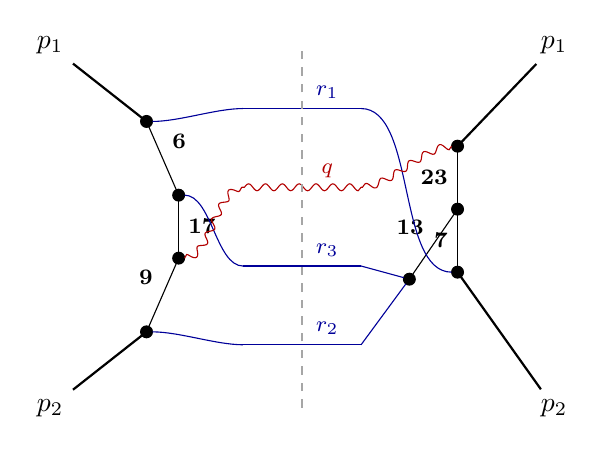
\begin{tikzpicture}
\begin{feynman}
\vertex (Lp1) at (-3.200,2.300) {$p_1$};
\vertex (Lp2) at (-3.200,-2.300) {$p_2$};
\vertex (Lcr1) at (-0.750,1.500);
\vertex (Lcr2) at (-0.750,-1.500);
\vertex (Lcr3) at (-0.750,-0.500);
\vertex (Lcq) at (-0.750,0.500);
\vertex[dot] (L6) at (-1.975,1.336) {};
\vertex[dot] (L17) at (-1.567,0.400) {};
\vertex[dot] (L9) at (-1.975,-1.336) {};
\vertex[dot] (Lroot) at (-1.567,-0.400) {};
\vertex (Rp1) at (3.200,2.300) {$p_1$};
\vertex (Rp2) at (3.200,-2.300) {$p_2$};
\vertex (Rcr1) at (0.750,1.500);
\vertex (Rcr2) at (0.750,-1.500);
\vertex (Rcr3) at (0.750,-0.500);
\vertex (Rcq) at (0.750,0.500);
\vertex[dot] (R7) at (1.975,-0.578) {};
\vertex[dot] (R23) at (1.975,0.222) {};
\vertex[dot] (R13) at (1.363,-0.667) {};
\vertex[dot] (Rroot) at (1.975,1.022) {};
\diagram* {
(L6) -- [plain, edge label={\footnotesize\bfseries 6}] (L17),
(L9) -- [plain, edge label={\footnotesize\bfseries 9}] (Lroot),
(L17) -- [plain, edge label={\footnotesize\bfseries 17}] (Lroot),
(Lp1) -- [plain, thick] (L6),
(Lp2) -- [plain, thick] (L9),
(Lcr1) -- [plain, blue!60!black, out=180, in=0, looseness=0.75] (L6),
(Lcr2) -- [plain, blue!60!black, out=180, in=0, looseness=0.75] (L9),
(Lcr3) -- [plain, blue!60!black, out=180, in=0, looseness=0.75] (L17),
(Lcq) -- [boson, red!70!black, out=180, in=0, looseness=0.75] (Lroot),
(R7) -- [plain, edge label={\footnotesize\bfseries 7}] (R23),
(R13) -- [plain, edge label={\footnotesize\bfseries 13}] (R23),
(R23) -- [plain, edge label={\footnotesize\bfseries 23}] (Rroot),
(Rp1) -- [plain, thick] (Rroot),
(Rp2) -- [plain, thick] (R7),
(Rcr1) -- [plain, blue!60!black, out=0, in=180, looseness=0.75] (R7),
(Rcr2) -- [plain, blue!60!black] (R13),
(Rcr3) -- [plain, blue!60!black] (R13),
(Rcq) -- [boson, red!70!black, out=0, in=180, looseness=0.75] (Rroot),
(Lcr1) -- [plain, blue!60!black] (Rcr1),
(Lcr2) -- [plain, blue!60!black] (Rcr2),
(Lcr3) -- [plain, blue!60!black] (Rcr3),
(Lcq) -- [boson, red!70!black] (Rcq),
};
\end{feynman}
\draw[dashed, gray!70] (0,-2.30) -- (0,2.30);
\node[font=\footnotesize, blue!60!black, above] at (0.32,1.50) {$r_1$};
\node[font=\footnotesize, blue!60!black, above] at (0.32,-1.50) {$r_2$};
\node[font=\footnotesize, blue!60!black, above] at (0.32,-0.50) {$r_3$};
\node[font=\footnotesize, red!70!black, above] at (0.32,0.50) {$q$};
\end{tikzpicture}}\\[2mm]\textbf{FAM[109]} (topo109)\\[2pt]{\footnotesize\begin{tabular}{@{}r@{\ \ }l@{\ \ }l@{}}\textbf{6} & $(p_1+r_1)^2$ & amplitude\\
\textbf{9} & $(p_2+r_2)^2$ & amplitude\\
\textbf{17} & $(p_1+r_1+r_3)^2$ & amplitude\\
\textbf{7} & $(p_2+r_1)^2$ & conjugate\\
\textbf{13} & $(r_2+r_3)^2$ & conjugate\\
\textbf{23} & $(p_2+r_1+r_2+r_3)^2$ & conjugate\\\end{tabular}}\\[2pt]{\scriptsize irreducible numerators: 14 = $(r_1+r_3)^2$}\end{minipage}\hfill%
\begin{minipage}[t]{0.48\textwidth}\centering\resizebox{0.9\linewidth}{!}{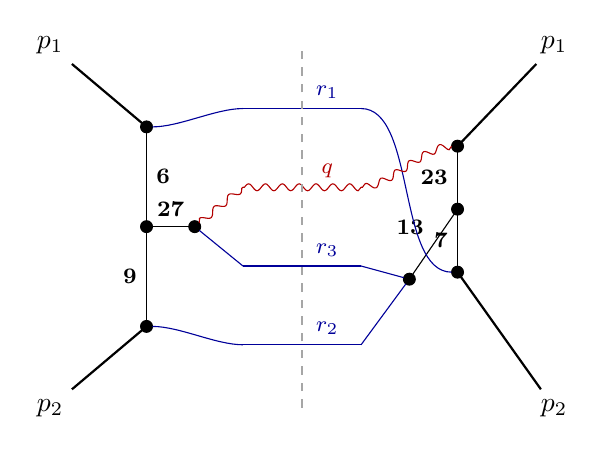
\begin{tikzpicture}
\begin{feynman}
\vertex (Lp1) at (-3.200,2.300) {$p_1$};
\vertex (Lp2) at (-3.200,-2.300) {$p_2$};
\vertex (Lcr1) at (-0.750,1.500);
\vertex (Lcr2) at (-0.750,-1.500);
\vertex (Lcr3) at (-0.750,-0.500);
\vertex (Lcq) at (-0.750,0.500);
\vertex[dot] (L6) at (-1.975,1.267) {};
\vertex[dot] (L27) at (-1.975,0.000) {};
\vertex[dot] (L9) at (-1.975,-1.267) {};
\vertex[dot] (Lroot) at (-1.363,0.000) {};
\vertex (Rp1) at (3.200,2.300) {$p_1$};
\vertex (Rp2) at (3.200,-2.300) {$p_2$};
\vertex (Rcr1) at (0.750,1.500);
\vertex (Rcr2) at (0.750,-1.500);
\vertex (Rcr3) at (0.750,-0.500);
\vertex (Rcq) at (0.750,0.500);
\vertex[dot] (R7) at (1.975,-0.578) {};
\vertex[dot] (R23) at (1.975,0.222) {};
\vertex[dot] (R13) at (1.363,-0.667) {};
\vertex[dot] (Rroot) at (1.975,1.022) {};
\diagram* {
(L6) -- [plain, edge label={\footnotesize\bfseries 6}] (L27),
(L9) -- [plain, edge label={\footnotesize\bfseries 9}] (L27),
(L27) -- [plain, edge label={\footnotesize\bfseries 27}] (Lroot),
(Lp1) -- [plain, thick] (L6),
(Lp2) -- [plain, thick] (L9),
(Lcr1) -- [plain, blue!60!black, out=180, in=0, looseness=0.75] (L6),
(Lcr2) -- [plain, blue!60!black, out=180, in=0, looseness=0.75] (L9),
(Lcr3) -- [plain, blue!60!black] (Lroot),
(Lcq) -- [boson, red!70!black] (Lroot),
(R7) -- [plain, edge label={\footnotesize\bfseries 7}] (R23),
(R13) -- [plain, edge label={\footnotesize\bfseries 13}] (R23),
(R23) -- [plain, edge label={\footnotesize\bfseries 23}] (Rroot),
(Rp1) -- [plain, thick] (Rroot),
(Rp2) -- [plain, thick] (R7),
(Rcr1) -- [plain, blue!60!black, out=0, in=180, looseness=0.75] (R7),
(Rcr2) -- [plain, blue!60!black] (R13),
(Rcr3) -- [plain, blue!60!black] (R13),
(Rcq) -- [boson, red!70!black, out=0, in=180, looseness=0.75] (Rroot),
(Lcr1) -- [plain, blue!60!black] (Rcr1),
(Lcr2) -- [plain, blue!60!black] (Rcr2),
(Lcr3) -- [plain, blue!60!black] (Rcr3),
(Lcq) -- [boson, red!70!black] (Rcq),
};
\end{feynman}
\draw[dashed, gray!70] (0,-2.30) -- (0,2.30);
\node[font=\footnotesize, blue!60!black, above] at (0.32,1.50) {$r_1$};
\node[font=\footnotesize, blue!60!black, above] at (0.32,-1.50) {$r_2$};
\node[font=\footnotesize, blue!60!black, above] at (0.32,-0.50) {$r_3$};
\node[font=\footnotesize, red!70!black, above] at (0.32,0.50) {$q$};
\end{tikzpicture}}\\[2mm]\textbf{FAM[115]} (topo115)\\[2pt]{\footnotesize\begin{tabular}{@{}r@{\ \ }l@{\ \ }l@{}}\textbf{6} & $(p_1+r_1)^2$ & amplitude\\
\textbf{9} & $(p_2+r_2)^2$ & amplitude\\
\textbf{27} & $(p_1+p_2+r_1+r_2)^2$ & amplitude\\
\textbf{7} & $(p_2+r_1)^2$ & conjugate\\
\textbf{13} & $(r_2+r_3)^2$ & conjugate\\
\textbf{23} & $(p_2+r_1+r_2+r_3)^2$ & conjugate\\\end{tabular}}\\[2pt]{\scriptsize irreducible numerators: 16 = $(p_2+r_1+r_2)^2$}\end{minipage}

\bigskip

\begin{minipage}[t]{0.48\textwidth}\centering\resizebox{0.9\linewidth}{!}{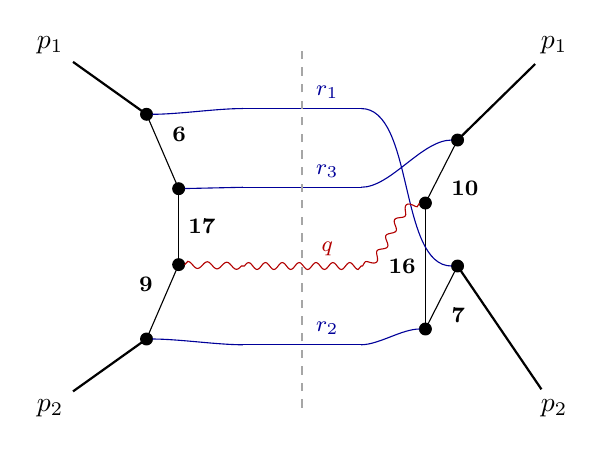
\begin{tikzpicture}
\begin{feynman}
\vertex (Lp1) at (-3.200,2.300) {$p_1$};
\vertex (Lp2) at (-3.200,-2.300) {$p_2$};
\vertex (Lcr1) at (-0.750,1.500);
\vertex (Lcr2) at (-0.750,-1.500);
\vertex (Lcr3) at (-0.750,0.500);
\vertex (Lcq) at (-0.750,-0.500);
\vertex[dot] (L6) at (-1.975,1.427) {};
\vertex[dot] (L17) at (-1.567,0.482) {};
\vertex[dot] (L9) at (-1.975,-1.427) {};
\vertex[dot] (Lroot) at (-1.567,-0.482) {};
\vertex (Rp1) at (3.200,2.300) {$p_1$};
\vertex (Rp2) at (3.200,-2.300) {$p_2$};
\vertex (Rcr1) at (0.750,1.500);
\vertex (Rcr2) at (0.750,-1.500);
\vertex (Rcr3) at (0.750,0.500);
\vertex (Rcq) at (0.750,-0.500);
\vertex[dot] (R7) at (1.975,-0.500) {};
\vertex[dot] (R16) at (1.567,-1.300) {};
\vertex[dot] (R10) at (1.975,1.100) {};
\vertex[dot] (Rroot) at (1.567,0.300) {};
\diagram* {
(L6) -- [plain, edge label={\footnotesize\bfseries 6}] (L17),
(L9) -- [plain, edge label={\footnotesize\bfseries 9}] (Lroot),
(L17) -- [plain, edge label={\footnotesize\bfseries 17}] (Lroot),
(Lp1) -- [plain, thick] (L6),
(Lp2) -- [plain, thick] (L9),
(Lcr1) -- [plain, blue!60!black, out=180, in=0, looseness=0.75] (L6),
(Lcr2) -- [plain, blue!60!black, out=180, in=0, looseness=0.75] (L9),
(Lcr3) -- [plain, blue!60!black] (L17),
(Lcq) -- [boson, red!70!black] (Lroot),
(R7) -- [plain, edge label={\footnotesize\bfseries 7}] (R16),
(R10) -- [plain, edge label={\footnotesize\bfseries 10}] (Rroot),
(R16) -- [plain, edge label={\footnotesize\bfseries 16}] (Rroot),
(Rp1) -- [plain, thick] (R10),
(Rp2) -- [plain, thick] (R7),
(Rcr1) -- [plain, blue!60!black, out=0, in=180, looseness=0.75] (R7),
(Rcr2) -- [plain, blue!60!black, out=0, in=180, looseness=0.75] (R16),
(Rcr3) -- [plain, blue!60!black, out=0, in=180, looseness=0.75] (R10),
(Rcq) -- [boson, red!70!black, out=0, in=180, looseness=0.75] (Rroot),
(Lcr1) -- [plain, blue!60!black] (Rcr1),
(Lcr2) -- [plain, blue!60!black] (Rcr2),
(Lcr3) -- [plain, blue!60!black] (Rcr3),
(Lcq) -- [boson, red!70!black] (Rcq),
};
\end{feynman}
\draw[dashed, gray!70] (0,-2.30) -- (0,2.30);
\node[font=\footnotesize, blue!60!black, above] at (0.32,1.50) {$r_1$};
\node[font=\footnotesize, blue!60!black, above] at (0.32,-1.50) {$r_2$};
\node[font=\footnotesize, blue!60!black, above] at (0.32,0.50) {$r_3$};
\node[font=\footnotesize, red!70!black, above] at (0.32,-0.50) {$q$};
\end{tikzpicture}}\\[2mm]\textbf{FAM[121]} (topo121)\\[2pt]{\footnotesize\begin{tabular}{@{}r@{\ \ }l@{\ \ }l@{}}\textbf{6} & $(p_1+r_1)^2$ & amplitude\\
\textbf{9} & $(p_2+r_2)^2$ & amplitude\\
\textbf{17} & $(p_1+r_1+r_3)^2$ & amplitude\\
\textbf{7} & $(p_2+r_1)^2$ & conjugate\\
\textbf{10} & $(p_1+r_3)^2$ & conjugate\\
\textbf{16} & $(p_2+r_1+r_2)^2$ & conjugate\\\end{tabular}}\\[2pt]{\scriptsize irreducible numerators: 23 = $(p_2+r_1+r_2+r_3)^2$}\end{minipage}\hfill%
\begin{minipage}[t]{0.48\textwidth}\centering\resizebox{0.9\linewidth}{!}{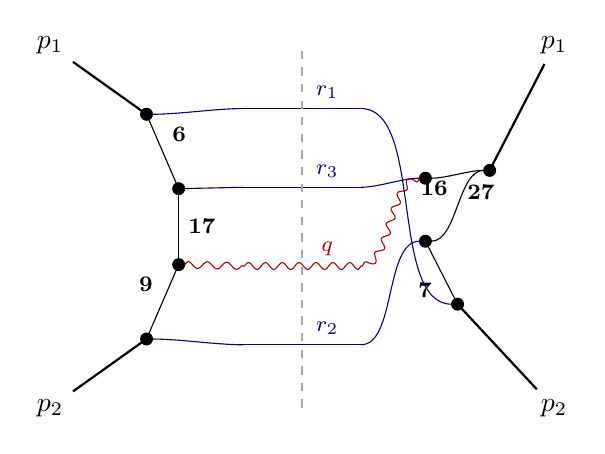
\begin{tikzpicture}
\begin{feynman}
\vertex (Lp1) at (-3.200,2.300) {$p_1$};
\vertex (Lp2) at (-3.200,-2.300) {$p_2$};
\vertex (Lcr1) at (-0.750,1.500);
\vertex (Lcr2) at (-0.750,-1.500);
\vertex (Lcr3) at (-0.750,0.500);
\vertex (Lcq) at (-0.750,-0.500);
\vertex[dot] (L6) at (-1.975,1.427) {};
\vertex[dot] (L17) at (-1.567,0.482) {};
\vertex[dot] (L9) at (-1.975,-1.427) {};
\vertex[dot] (Lroot) at (-1.567,-0.482) {};
\vertex (Rp1) at (3.200,2.300) {$p_1$};
\vertex (Rp2) at (3.200,-2.300) {$p_2$};
\vertex (Rcr1) at (0.750,1.500);
\vertex (Rcr2) at (0.750,-1.500);
\vertex (Rcr3) at (0.750,0.500);
\vertex (Rcq) at (0.750,-0.500);
\vertex[dot] (R7) at (1.975,-0.985) {};
\vertex[dot] (R16) at (1.567,-0.185) {};
\vertex[dot] (R27) at (2.383,0.715) {};
\vertex[dot] (Rroot) at (1.567,0.615) {};
\diagram* {
(L6) -- [plain, edge label={\footnotesize\bfseries 6}] (L17),
(L9) -- [plain, edge label={\footnotesize\bfseries 9}] (Lroot),
(L17) -- [plain, edge label={\footnotesize\bfseries 17}] (Lroot),
(Lp1) -- [plain, thick] (L6),
(Lp2) -- [plain, thick] (L9),
(Lcr1) -- [plain, blue!60!black, out=180, in=0, looseness=0.75] (L6),
(Lcr2) -- [plain, blue!60!black, out=180, in=0, looseness=0.75] (L9),
(Lcr3) -- [plain, blue!60!black] (L17),
(Lcq) -- [boson, red!70!black] (Lroot),
(R7) -- [plain, edge label={\footnotesize\bfseries 7}] (R16),
(R16) -- [plain, out=0, in=180, looseness=0.75, edge label={\footnotesize\bfseries 16}] (R27),
(R27) -- [plain, out=180, in=0, looseness=0.75, edge label={\footnotesize\bfseries 27}] (Rroot),
(Rp1) -- [plain, thick] (R27),
(Rp2) -- [plain, thick] (R7),
(Rcr1) -- [plain, blue!60!black, out=0, in=180, looseness=0.75] (R7),
(Rcr2) -- [plain, blue!60!black, out=0, in=180, looseness=0.75] (R16),
(Rcr3) -- [plain, blue!60!black, out=0, in=180, looseness=0.75] (Rroot),
(Rcq) -- [boson, red!70!black, out=0, in=180, looseness=0.75] (Rroot),
(Lcr1) -- [plain, blue!60!black] (Rcr1),
(Lcr2) -- [plain, blue!60!black] (Rcr2),
(Lcr3) -- [plain, blue!60!black] (Rcr3),
(Lcq) -- [boson, red!70!black] (Rcq),
};
\end{feynman}
\draw[dashed, gray!70] (0,-2.30) -- (0,2.30);
\node[font=\footnotesize, blue!60!black, above] at (0.32,1.50) {$r_1$};
\node[font=\footnotesize, blue!60!black, above] at (0.32,-1.50) {$r_2$};
\node[font=\footnotesize, blue!60!black, above] at (0.32,0.50) {$r_3$};
\node[font=\footnotesize, red!70!black, above] at (0.32,-0.50) {$q$};
\end{tikzpicture}}\\[2mm]\textbf{FAM[127]} (topo127)\\[2pt]{\footnotesize\begin{tabular}{@{}r@{\ \ }l@{\ \ }l@{}}\textbf{6} & $(p_1+r_1)^2$ & amplitude\\
\textbf{9} & $(p_2+r_2)^2$ & amplitude\\
\textbf{17} & $(p_1+r_1+r_3)^2$ & amplitude\\
\textbf{7} & $(p_2+r_1)^2$ & conjugate\\
\textbf{16} & $(p_2+r_1+r_2)^2$ & conjugate\\
\textbf{27} & $(p_1+p_2+r_1+r_2)^2$ & conjugate\\\end{tabular}}\\[2pt]{\scriptsize irreducible numerators: 22 = $(p_1+r_1+r_2+r_3)^2$}\end{minipage}

\bigskip

\begin{minipage}[t]{0.48\textwidth}\centering\resizebox{0.9\linewidth}{!}{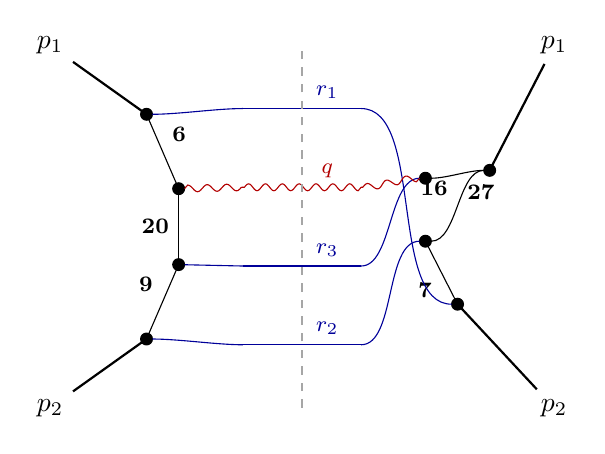
\begin{tikzpicture}
\begin{feynman}
\vertex (Lp1) at (-3.200,2.300) {$p_1$};
\vertex (Lp2) at (-3.200,-2.300) {$p_2$};
\vertex (Lcr1) at (-0.750,1.500);
\vertex (Lcr2) at (-0.750,-1.500);
\vertex (Lcr3) at (-0.750,-0.500);
\vertex (Lcq) at (-0.750,0.500);
\vertex[dot] (L6) at (-1.975,1.427) {};
\vertex[dot] (Lroot) at (-1.567,0.482) {};
\vertex[dot] (L9) at (-1.975,-1.427) {};
\vertex[dot] (L20) at (-1.567,-0.482) {};
\vertex (Rp1) at (3.200,2.300) {$p_1$};
\vertex (Rp2) at (3.200,-2.300) {$p_2$};
\vertex (Rcr1) at (0.750,1.500);
\vertex (Rcr2) at (0.750,-1.500);
\vertex (Rcr3) at (0.750,-0.500);
\vertex (Rcq) at (0.750,0.500);
\vertex[dot] (R7) at (1.975,-0.985) {};
\vertex[dot] (R16) at (1.567,-0.185) {};
\vertex[dot] (R27) at (2.383,0.715) {};
\vertex[dot] (Rroot) at (1.567,0.615) {};
\diagram* {
(L6) -- [plain, edge label={\footnotesize\bfseries 6}] (Lroot),
(L9) -- [plain, edge label={\footnotesize\bfseries 9}] (L20),
(L20) -- [plain, edge label={\footnotesize\bfseries 20}] (Lroot),
(Lp1) -- [plain, thick] (L6),
(Lp2) -- [plain, thick] (L9),
(Lcr1) -- [plain, blue!60!black, out=180, in=0, looseness=0.75] (L6),
(Lcr2) -- [plain, blue!60!black, out=180, in=0, looseness=0.75] (L9),
(Lcr3) -- [plain, blue!60!black] (L20),
(Lcq) -- [boson, red!70!black] (Lroot),
(R7) -- [plain, edge label={\footnotesize\bfseries 7}] (R16),
(R16) -- [plain, out=0, in=180, looseness=0.75, edge label={\footnotesize\bfseries 16}] (R27),
(R27) -- [plain, out=180, in=0, looseness=0.75, edge label={\footnotesize\bfseries 27}] (Rroot),
(Rp1) -- [plain, thick] (R27),
(Rp2) -- [plain, thick] (R7),
(Rcr1) -- [plain, blue!60!black, out=0, in=180, looseness=0.75] (R7),
(Rcr2) -- [plain, blue!60!black, out=0, in=180, looseness=0.75] (R16),
(Rcr3) -- [plain, blue!60!black, out=0, in=180, looseness=0.75] (Rroot),
(Rcq) -- [boson, red!70!black, out=0, in=180, looseness=0.75] (Rroot),
(Lcr1) -- [plain, blue!60!black] (Rcr1),
(Lcr2) -- [plain, blue!60!black] (Rcr2),
(Lcr3) -- [plain, blue!60!black] (Rcr3),
(Lcq) -- [boson, red!70!black] (Rcq),
};
\end{feynman}
\draw[dashed, gray!70] (0,-2.30) -- (0,2.30);
\node[font=\footnotesize, blue!60!black, above] at (0.32,1.50) {$r_1$};
\node[font=\footnotesize, blue!60!black, above] at (0.32,-1.50) {$r_2$};
\node[font=\footnotesize, blue!60!black, above] at (0.32,-0.50) {$r_3$};
\node[font=\footnotesize, red!70!black, above] at (0.32,0.50) {$q$};
\end{tikzpicture}}\\[2mm]\textbf{FAM[133]} (topo133)\\[2pt]{\footnotesize\begin{tabular}{@{}r@{\ \ }l@{\ \ }l@{}}\textbf{6} & $(p_1+r_1)^2$ & amplitude\\
\textbf{9} & $(p_2+r_2)^2$ & amplitude\\
\textbf{20} & $(p_2+r_2+r_3)^2$ & amplitude\\
\textbf{7} & $(p_2+r_1)^2$ & conjugate\\
\textbf{16} & $(p_2+r_1+r_2)^2$ & conjugate\\
\textbf{27} & $(p_1+p_2+r_1+r_2)^2$ & conjugate\\\end{tabular}}\\[2pt]{\scriptsize irreducible numerators: 13 = $(r_2+r_3)^2$}\end{minipage}\hfill%
\begin{minipage}[t]{0.48\textwidth}\centering\resizebox{0.9\linewidth}{!}{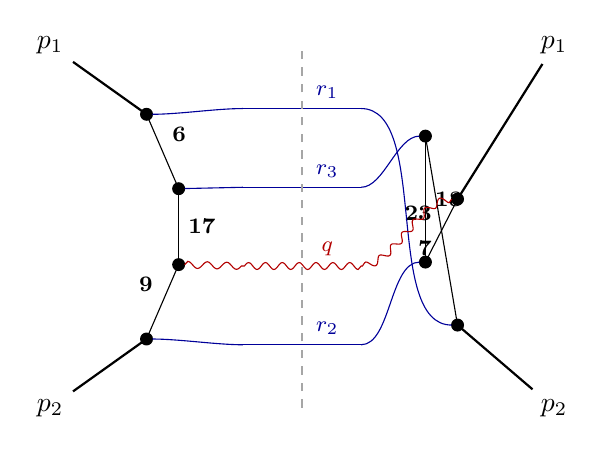
\begin{tikzpicture}
\begin{feynman}
\vertex (Lp1) at (-3.200,2.300) {$p_1$};
\vertex (Lp2) at (-3.200,-2.300) {$p_2$};
\vertex (Lcr1) at (-0.750,1.500);
\vertex (Lcr2) at (-0.750,-1.500);
\vertex (Lcr3) at (-0.750,0.500);
\vertex (Lcq) at (-0.750,-0.500);
\vertex[dot] (L6) at (-1.975,1.427) {};
\vertex[dot] (L17) at (-1.567,0.482) {};
\vertex[dot] (L9) at (-1.975,-1.427) {};
\vertex[dot] (Lroot) at (-1.567,-0.482) {};
\vertex (Rp1) at (3.200,2.300) {$p_1$};
\vertex (Rp2) at (3.200,-2.300) {$p_2$};
\vertex (Rcr1) at (0.750,1.500);
\vertex (Rcr2) at (0.750,-1.500);
\vertex (Rcr3) at (0.750,0.500);
\vertex (Rcq) at (0.750,-0.500);
\vertex[dot] (R7) at (1.975,-1.250) {};
\vertex[dot] (R18) at (1.567,1.150) {};
\vertex[dot] (R23) at (1.567,-0.450) {};
\vertex[dot] (Rroot) at (1.975,0.350) {};
\diagram* {
(L6) -- [plain, edge label={\footnotesize\bfseries 6}] (L17),
(L9) -- [plain, edge label={\footnotesize\bfseries 9}] (Lroot),
(L17) -- [plain, edge label={\footnotesize\bfseries 17}] (Lroot),
(Lp1) -- [plain, thick] (L6),
(Lp2) -- [plain, thick] (L9),
(Lcr1) -- [plain, blue!60!black, out=180, in=0, looseness=0.75] (L6),
(Lcr2) -- [plain, blue!60!black, out=180, in=0, looseness=0.75] (L9),
(Lcr3) -- [plain, blue!60!black] (L17),
(Lcq) -- [boson, red!70!black] (Lroot),
(R7) -- [plain, edge label={\footnotesize\bfseries 7}] (R18),
(R18) -- [plain, edge label={\footnotesize\bfseries 18}] (R23),
(R23) -- [plain, edge label={\footnotesize\bfseries 23}] (Rroot),
(Rp1) -- [plain, thick] (Rroot),
(Rp2) -- [plain, thick] (R7),
(Rcr1) -- [plain, blue!60!black, out=0, in=180, looseness=0.75] (R7),
(Rcr2) -- [plain, blue!60!black, out=0, in=180, looseness=0.75] (R23),
(Rcr3) -- [plain, blue!60!black, out=0, in=180, looseness=0.75] (R18),
(Rcq) -- [boson, red!70!black, out=0, in=180, looseness=0.75] (Rroot),
(Lcr1) -- [plain, blue!60!black] (Rcr1),
(Lcr2) -- [plain, blue!60!black] (Rcr2),
(Lcr3) -- [plain, blue!60!black] (Rcr3),
(Lcq) -- [boson, red!70!black] (Rcq),
};
\end{feynman}
\draw[dashed, gray!70] (0,-2.30) -- (0,2.30);
\node[font=\footnotesize, blue!60!black, above] at (0.32,1.50) {$r_1$};
\node[font=\footnotesize, blue!60!black, above] at (0.32,-1.50) {$r_2$};
\node[font=\footnotesize, blue!60!black, above] at (0.32,0.50) {$r_3$};
\node[font=\footnotesize, red!70!black, above] at (0.32,-0.50) {$q$};
\end{tikzpicture}}\\[2mm]\textbf{FAM[139]} (topo139)\\[2pt]{\footnotesize\begin{tabular}{@{}r@{\ \ }l@{\ \ }l@{}}\textbf{6} & $(p_1+r_1)^2$ & amplitude\\
\textbf{9} & $(p_2+r_2)^2$ & amplitude\\
\textbf{17} & $(p_1+r_1+r_3)^2$ & amplitude\\
\textbf{7} & $(p_2+r_1)^2$ & conjugate\\
\textbf{18} & $(p_2+r_1+r_3)^2$ & conjugate\\
\textbf{23} & $(p_2+r_1+r_2+r_3)^2$ & conjugate\\\end{tabular}}\\[2pt]{\scriptsize irreducible numerators: 20 = $(p_2+r_2+r_3)^2$}\end{minipage}

\bigskip

\begin{minipage}[t]{0.48\textwidth}\centering\resizebox{0.9\linewidth}{!}{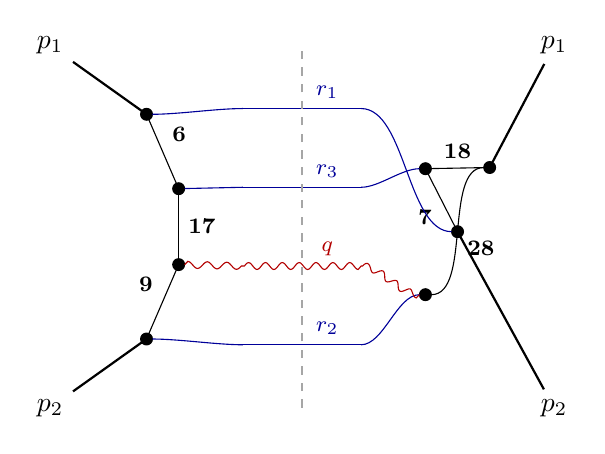
\begin{tikzpicture}
\begin{feynman}
\vertex (Lp1) at (-3.200,2.300) {$p_1$};
\vertex (Lp2) at (-3.200,-2.300) {$p_2$};
\vertex (Lcr1) at (-0.750,1.500);
\vertex (Lcr2) at (-0.750,-1.500);
\vertex (Lcr3) at (-0.750,0.500);
\vertex (Lcq) at (-0.750,-0.500);
\vertex[dot] (L6) at (-1.975,1.427) {};
\vertex[dot] (L17) at (-1.567,0.482) {};
\vertex[dot] (L9) at (-1.975,-1.427) {};
\vertex[dot] (Lroot) at (-1.567,-0.482) {};
\vertex (Rp1) at (3.200,2.300) {$p_1$};
\vertex (Rp2) at (3.200,-2.300) {$p_2$};
\vertex (Rcr1) at (0.750,1.500);
\vertex (Rcr2) at (0.750,-1.500);
\vertex (Rcr3) at (0.750,0.500);
\vertex (Rcq) at (0.750,-0.500);
\vertex[dot] (R7) at (1.975,-0.064) {};
\vertex[dot] (R18) at (1.567,0.736) {};
\vertex[dot] (R28) at (2.383,0.751) {};
\vertex[dot] (Rroot) at (1.567,-0.864) {};
\diagram* {
(L6) -- [plain, edge label={\footnotesize\bfseries 6}] (L17),
(L9) -- [plain, edge label={\footnotesize\bfseries 9}] (Lroot),
(L17) -- [plain, edge label={\footnotesize\bfseries 17}] (Lroot),
(Lp1) -- [plain, thick] (L6),
(Lp2) -- [plain, thick] (L9),
(Lcr1) -- [plain, blue!60!black, out=180, in=0, looseness=0.75] (L6),
(Lcr2) -- [plain, blue!60!black, out=180, in=0, looseness=0.75] (L9),
(Lcr3) -- [plain, blue!60!black] (L17),
(Lcq) -- [boson, red!70!black] (Lroot),
(R7) -- [plain, edge label={\footnotesize\bfseries 7}] (R18),
(R18) -- [plain, edge label={\footnotesize\bfseries 18}] (R28),
(R28) -- [plain, out=180, in=0, looseness=0.75, edge label={\footnotesize\bfseries 28}] (Rroot),
(Rp1) -- [plain, thick] (R28),
(Rp2) -- [plain, thick] (R7),
(Rcr1) -- [plain, blue!60!black, out=0, in=180, looseness=0.75] (R7),
(Rcr2) -- [plain, blue!60!black, out=0, in=180, looseness=0.75] (Rroot),
(Rcr3) -- [plain, blue!60!black, out=0, in=180, looseness=0.75] (R18),
(Rcq) -- [boson, red!70!black, out=0, in=180, looseness=0.75] (Rroot),
(Lcr1) -- [plain, blue!60!black] (Rcr1),
(Lcr2) -- [plain, blue!60!black] (Rcr2),
(Lcr3) -- [plain, blue!60!black] (Rcr3),
(Lcq) -- [boson, red!70!black] (Rcq),
};
\end{feynman}
\draw[dashed, gray!70] (0,-2.30) -- (0,2.30);
\node[font=\footnotesize, blue!60!black, above] at (0.32,1.50) {$r_1$};
\node[font=\footnotesize, blue!60!black, above] at (0.32,-1.50) {$r_2$};
\node[font=\footnotesize, blue!60!black, above] at (0.32,0.50) {$r_3$};
\node[font=\footnotesize, red!70!black, above] at (0.32,-0.50) {$q$};
\end{tikzpicture}}\\[2mm]\textbf{FAM[145]} (topo145)\\[2pt]{\footnotesize\begin{tabular}{@{}r@{\ \ }l@{\ \ }l@{}}\textbf{6} & $(p_1+r_1)^2$ & amplitude\\
\textbf{9} & $(p_2+r_2)^2$ & amplitude\\
\textbf{17} & $(p_1+r_1+r_3)^2$ & amplitude\\
\textbf{7} & $(p_2+r_1)^2$ & conjugate\\
\textbf{18} & $(p_2+r_1+r_3)^2$ & conjugate\\
\textbf{28} & $(p_1+p_2+r_1+r_3)^2$ & conjugate\\\end{tabular}}\\[2pt]{\scriptsize irreducible numerators: 20 = $(p_2+r_2+r_3)^2$}\end{minipage}\hfill%
\begin{minipage}[t]{0.48\textwidth}\centering\resizebox{0.9\linewidth}{!}{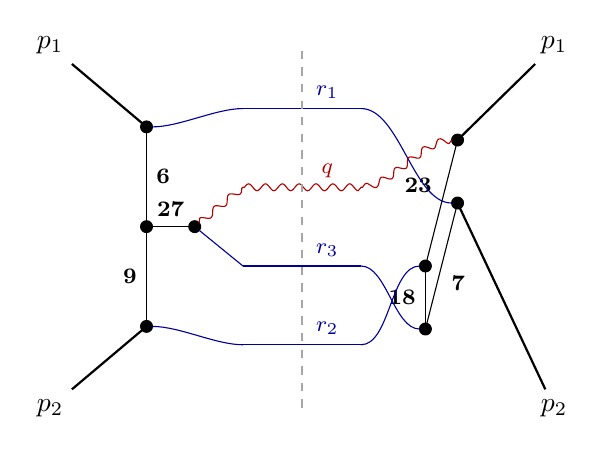
\begin{tikzpicture}
\begin{feynman}
\vertex (Lp1) at (-3.200,2.300) {$p_1$};
\vertex (Lp2) at (-3.200,-2.300) {$p_2$};
\vertex (Lcr1) at (-0.750,1.500);
\vertex (Lcr2) at (-0.750,-1.500);
\vertex (Lcr3) at (-0.750,-0.500);
\vertex (Lcq) at (-0.750,0.500);
\vertex[dot] (L6) at (-1.975,1.267) {};
\vertex[dot] (L27) at (-1.975,0.000) {};
\vertex[dot] (L9) at (-1.975,-1.267) {};
\vertex[dot] (Lroot) at (-1.363,0.000) {};
\vertex (Rp1) at (3.200,2.300) {$p_1$};
\vertex (Rp2) at (3.200,-2.300) {$p_2$};
\vertex (Rcr1) at (0.750,1.500);
\vertex (Rcr2) at (0.750,-1.500);
\vertex (Rcr3) at (0.750,-0.500);
\vertex (Rcq) at (0.750,0.500);
\vertex[dot] (R7) at (1.975,0.300) {};
\vertex[dot] (R18) at (1.567,-1.300) {};
\vertex[dot] (R23) at (1.567,-0.500) {};
\vertex[dot] (Rroot) at (1.975,1.100) {};
\diagram* {
(L6) -- [plain, edge label={\footnotesize\bfseries 6}] (L27),
(L9) -- [plain, edge label={\footnotesize\bfseries 9}] (L27),
(L27) -- [plain, edge label={\footnotesize\bfseries 27}] (Lroot),
(Lp1) -- [plain, thick] (L6),
(Lp2) -- [plain, thick] (L9),
(Lcr1) -- [plain, blue!60!black, out=180, in=0, looseness=0.75] (L6),
(Lcr2) -- [plain, blue!60!black, out=180, in=0, looseness=0.75] (L9),
(Lcr3) -- [plain, blue!60!black] (Lroot),
(Lcq) -- [boson, red!70!black] (Lroot),
(R7) -- [plain, edge label={\footnotesize\bfseries 7}] (R18),
(R18) -- [plain, edge label={\footnotesize\bfseries 18}] (R23),
(R23) -- [plain, edge label={\footnotesize\bfseries 23}] (Rroot),
(Rp1) -- [plain, thick] (Rroot),
(Rp2) -- [plain, thick] (R7),
(Rcr1) -- [plain, blue!60!black, out=0, in=180, looseness=0.75] (R7),
(Rcr2) -- [plain, blue!60!black, out=0, in=180, looseness=0.75] (R23),
(Rcr3) -- [plain, blue!60!black, out=0, in=180, looseness=0.75] (R18),
(Rcq) -- [boson, red!70!black, out=0, in=180, looseness=0.75] (Rroot),
(Lcr1) -- [plain, blue!60!black] (Rcr1),
(Lcr2) -- [plain, blue!60!black] (Rcr2),
(Lcr3) -- [plain, blue!60!black] (Rcr3),
(Lcq) -- [boson, red!70!black] (Rcq),
};
\end{feynman}
\draw[dashed, gray!70] (0,-2.30) -- (0,2.30);
\node[font=\footnotesize, blue!60!black, above] at (0.32,1.50) {$r_1$};
\node[font=\footnotesize, blue!60!black, above] at (0.32,-1.50) {$r_2$};
\node[font=\footnotesize, blue!60!black, above] at (0.32,-0.50) {$r_3$};
\node[font=\footnotesize, red!70!black, above] at (0.32,0.50) {$q$};
\end{tikzpicture}}\\[2mm]\textbf{FAM[151]} (topo151)\\[2pt]{\footnotesize\begin{tabular}{@{}r@{\ \ }l@{\ \ }l@{}}\textbf{6} & $(p_1+r_1)^2$ & amplitude\\
\textbf{9} & $(p_2+r_2)^2$ & amplitude\\
\textbf{27} & $(p_1+p_2+r_1+r_2)^2$ & amplitude\\
\textbf{7} & $(p_2+r_1)^2$ & conjugate\\
\textbf{18} & $(p_2+r_1+r_3)^2$ & conjugate\\
\textbf{23} & $(p_2+r_1+r_2+r_3)^2$ & conjugate\\\end{tabular}}\\[2pt]{\scriptsize irreducible numerators: 25 = $(p_1+p_2+r_2)^2$}\end{minipage}

\bigskip

\begin{minipage}[t]{0.48\textwidth}\centering\resizebox{0.9\linewidth}{!}{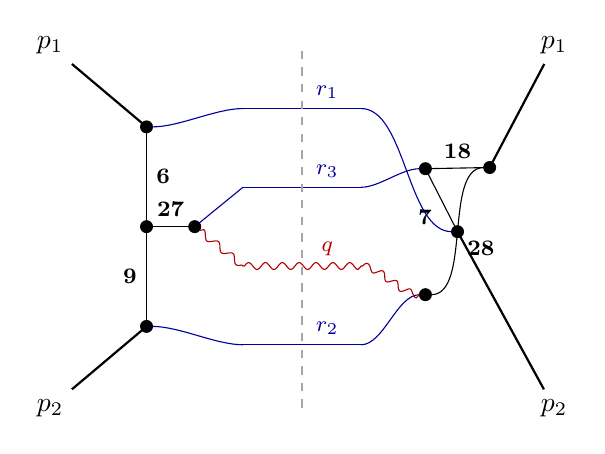
\begin{tikzpicture}
\begin{feynman}
\vertex (Lp1) at (-3.200,2.300) {$p_1$};
\vertex (Lp2) at (-3.200,-2.300) {$p_2$};
\vertex (Lcr1) at (-0.750,1.500);
\vertex (Lcr2) at (-0.750,-1.500);
\vertex (Lcr3) at (-0.750,0.500);
\vertex (Lcq) at (-0.750,-0.500);
\vertex[dot] (L6) at (-1.975,1.267) {};
\vertex[dot] (L27) at (-1.975,0.000) {};
\vertex[dot] (L9) at (-1.975,-1.267) {};
\vertex[dot] (Lroot) at (-1.363,0.000) {};
\vertex (Rp1) at (3.200,2.300) {$p_1$};
\vertex (Rp2) at (3.200,-2.300) {$p_2$};
\vertex (Rcr1) at (0.750,1.500);
\vertex (Rcr2) at (0.750,-1.500);
\vertex (Rcr3) at (0.750,0.500);
\vertex (Rcq) at (0.750,-0.500);
\vertex[dot] (R7) at (1.975,-0.064) {};
\vertex[dot] (R18) at (1.567,0.736) {};
\vertex[dot] (R28) at (2.383,0.751) {};
\vertex[dot] (Rroot) at (1.567,-0.864) {};
\diagram* {
(L6) -- [plain, edge label={\footnotesize\bfseries 6}] (L27),
(L9) -- [plain, edge label={\footnotesize\bfseries 9}] (L27),
(L27) -- [plain, edge label={\footnotesize\bfseries 27}] (Lroot),
(Lp1) -- [plain, thick] (L6),
(Lp2) -- [plain, thick] (L9),
(Lcr1) -- [plain, blue!60!black, out=180, in=0, looseness=0.75] (L6),
(Lcr2) -- [plain, blue!60!black, out=180, in=0, looseness=0.75] (L9),
(Lcr3) -- [plain, blue!60!black] (Lroot),
(Lcq) -- [boson, red!70!black] (Lroot),
(R7) -- [plain, edge label={\footnotesize\bfseries 7}] (R18),
(R18) -- [plain, edge label={\footnotesize\bfseries 18}] (R28),
(R28) -- [plain, out=180, in=0, looseness=0.75, edge label={\footnotesize\bfseries 28}] (Rroot),
(Rp1) -- [plain, thick] (R28),
(Rp2) -- [plain, thick] (R7),
(Rcr1) -- [plain, blue!60!black, out=0, in=180, looseness=0.75] (R7),
(Rcr2) -- [plain, blue!60!black, out=0, in=180, looseness=0.75] (Rroot),
(Rcr3) -- [plain, blue!60!black, out=0, in=180, looseness=0.75] (R18),
(Rcq) -- [boson, red!70!black, out=0, in=180, looseness=0.75] (Rroot),
(Lcr1) -- [plain, blue!60!black] (Rcr1),
(Lcr2) -- [plain, blue!60!black] (Rcr2),
(Lcr3) -- [plain, blue!60!black] (Rcr3),
(Lcq) -- [boson, red!70!black] (Rcq),
};
\end{feynman}
\draw[dashed, gray!70] (0,-2.30) -- (0,2.30);
\node[font=\footnotesize, blue!60!black, above] at (0.32,1.50) {$r_1$};
\node[font=\footnotesize, blue!60!black, above] at (0.32,-1.50) {$r_2$};
\node[font=\footnotesize, blue!60!black, above] at (0.32,0.50) {$r_3$};
\node[font=\footnotesize, red!70!black, above] at (0.32,-0.50) {$q$};
\end{tikzpicture}}\\[2mm]\textbf{FAM[157]} (topo157)\\[2pt]{\footnotesize\begin{tabular}{@{}r@{\ \ }l@{\ \ }l@{}}\textbf{6} & $(p_1+r_1)^2$ & amplitude\\
\textbf{9} & $(p_2+r_2)^2$ & amplitude\\
\textbf{27} & $(p_1+p_2+r_1+r_2)^2$ & amplitude\\
\textbf{7} & $(p_2+r_1)^2$ & conjugate\\
\textbf{18} & $(p_2+r_1+r_3)^2$ & conjugate\\
\textbf{28} & $(p_1+p_2+r_1+r_3)^2$ & conjugate\\\end{tabular}}\\[2pt]{\scriptsize irreducible numerators: 14 = $(r_1+r_3)^2$}\end{minipage}\hfill%
\begin{minipage}[t]{0.48\textwidth}\centering\resizebox{0.9\linewidth}{!}{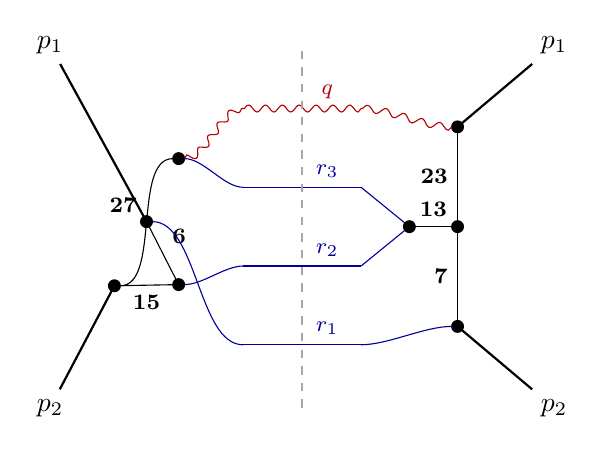
\begin{tikzpicture}
\begin{feynman}
\vertex (Lp1) at (-3.200,2.300) {$p_1$};
\vertex (Lp2) at (-3.200,-2.300) {$p_2$};
\vertex (Lcr1) at (-0.750,-1.500);
\vertex (Lcr2) at (-0.750,-0.500);
\vertex (Lcr3) at (-0.750,0.500);
\vertex (Lcq) at (-0.750,1.500);
\vertex[dot] (L6) at (-1.975,0.064) {};
\vertex[dot] (L15) at (-1.567,-0.736) {};
\vertex[dot] (L27) at (-2.383,-0.751) {};
\vertex[dot] (Lroot) at (-1.567,0.864) {};
\vertex (Rp1) at (3.200,2.300) {$p_1$};
\vertex (Rp2) at (3.200,-2.300) {$p_2$};
\vertex (Rcr1) at (0.750,-1.500);
\vertex (Rcr2) at (0.750,-0.500);
\vertex (Rcr3) at (0.750,0.500);
\vertex (Rcq) at (0.750,1.500);
\vertex[dot] (R7) at (1.975,-1.267) {};
\vertex[dot] (R23) at (1.975,0.000) {};
\vertex[dot] (R13) at (1.363,0.000) {};
\vertex[dot] (Rroot) at (1.975,1.267) {};
\diagram* {
(L6) -- [plain, edge label={\footnotesize\bfseries 6}] (L15),
(L15) -- [plain, edge label={\footnotesize\bfseries 15}] (L27),
(L27) -- [plain, out=0, in=180, looseness=0.75, edge label={\footnotesize\bfseries 27}] (Lroot),
(Lp1) -- [plain, thick] (L6),
(Lp2) -- [plain, thick] (L27),
(Lcr1) -- [plain, blue!60!black, out=180, in=0, looseness=0.75] (L6),
(Lcr2) -- [plain, blue!60!black, out=180, in=0, looseness=0.75] (L15),
(Lcr3) -- [plain, blue!60!black, out=180, in=0, looseness=0.75] (Lroot),
(Lcq) -- [boson, red!70!black, out=180, in=0, looseness=0.75] (Lroot),
(R7) -- [plain, edge label={\footnotesize\bfseries 7}] (R23),
(R13) -- [plain, edge label={\footnotesize\bfseries 13}] (R23),
(R23) -- [plain, edge label={\footnotesize\bfseries 23}] (Rroot),
(Rp1) -- [plain, thick] (Rroot),
(Rp2) -- [plain, thick] (R7),
(Rcr1) -- [plain, blue!60!black, out=0, in=180, looseness=0.75] (R7),
(Rcr2) -- [plain, blue!60!black] (R13),
(Rcr3) -- [plain, blue!60!black] (R13),
(Rcq) -- [boson, red!70!black, out=0, in=180, looseness=0.75] (Rroot),
(Lcr1) -- [plain, blue!60!black] (Rcr1),
(Lcr2) -- [plain, blue!60!black] (Rcr2),
(Lcr3) -- [plain, blue!60!black] (Rcr3),
(Lcq) -- [boson, red!70!black] (Rcq),
};
\end{feynman}
\draw[dashed, gray!70] (0,-2.30) -- (0,2.30);
\node[font=\footnotesize, blue!60!black, above] at (0.32,-1.50) {$r_1$};
\node[font=\footnotesize, blue!60!black, above] at (0.32,-0.50) {$r_2$};
\node[font=\footnotesize, blue!60!black, above] at (0.32,0.50) {$r_3$};
\node[font=\footnotesize, red!70!black, above] at (0.32,1.50) {$q$};
\end{tikzpicture}}\\[2mm]\textbf{FAM[163]} (topo163)\\[2pt]{\footnotesize\begin{tabular}{@{}r@{\ \ }l@{\ \ }l@{}}\textbf{6} & $(p_1+r_1)^2$ & amplitude\\
\textbf{15} & $(p_1+r_1+r_2)^2$ & amplitude\\
\textbf{27} & $(p_1+p_2+r_1+r_2)^2$ & amplitude\\
\textbf{7} & $(p_2+r_1)^2$ & conjugate\\
\textbf{13} & $(r_2+r_3)^2$ & conjugate\\
\textbf{23} & $(p_2+r_1+r_2+r_3)^2$ & conjugate\\\end{tabular}}\\[2pt]{\scriptsize irreducible numerators: 12 = $(r_1+r_2)^2$}\end{minipage}

\bigskip

\begin{minipage}[t]{0.48\textwidth}\centering\resizebox{0.9\linewidth}{!}{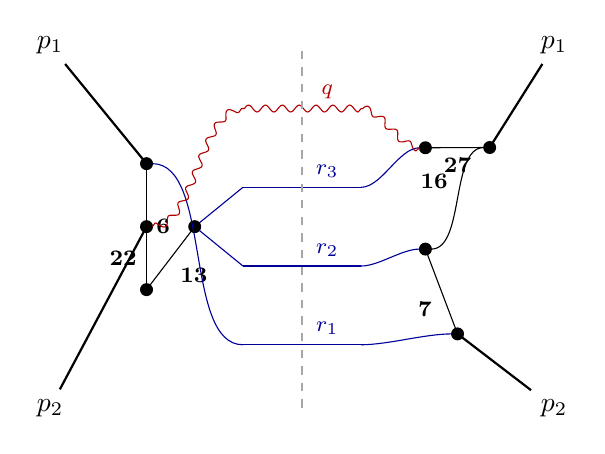
\begin{tikzpicture}
\begin{feynman}
\vertex (Lp1) at (-3.200,2.300) {$p_1$};
\vertex (Lp2) at (-3.200,-2.300) {$p_2$};
\vertex (Lcr1) at (-0.750,-1.500);
\vertex (Lcr2) at (-0.750,-0.500);
\vertex (Lcr3) at (-0.750,0.500);
\vertex (Lcq) at (-0.750,1.500);
\vertex[dot] (L6) at (-1.975,0.800) {};
\vertex[dot] (L22) at (-1.975,-0.800) {};
\vertex[dot] (L13) at (-1.363,0.000) {};
\vertex[dot] (Lroot) at (-1.975,0.000) {};
\vertex (Rp1) at (3.200,2.300) {$p_1$};
\vertex (Rp2) at (3.200,-2.300) {$p_2$};
\vertex (Rcr1) at (0.750,-1.500);
\vertex (Rcr2) at (0.750,-0.500);
\vertex (Rcr3) at (0.750,0.500);
\vertex (Rcq) at (0.750,1.500);
\vertex[dot] (R7) at (1.975,-1.362) {};
\vertex[dot] (R16) at (1.567,-0.285) {};
\vertex[dot] (R27) at (2.383,1.005) {};
\vertex[dot] (Rroot) at (1.567,1.002) {};
\diagram* {
(L6) -- [plain, edge label={\footnotesize\bfseries 6}] (L22),
(L13) -- [plain, edge label={\footnotesize\bfseries 13}] (L22),
(L22) -- [plain, edge label={\footnotesize\bfseries 22}] (Lroot),
(Lp1) -- [plain, thick] (L6),
(Lp2) -- [plain, thick] (Lroot),
(Lcr1) -- [plain, blue!60!black, out=180, in=0, looseness=0.75] (L6),
(Lcr2) -- [plain, blue!60!black] (L13),
(Lcr3) -- [plain, blue!60!black] (L13),
(Lcq) -- [boson, red!70!black, out=180, in=0, looseness=0.75] (Lroot),
(R7) -- [plain, edge label={\footnotesize\bfseries 7}] (R16),
(R16) -- [plain, out=0, in=180, looseness=0.75, edge label={\footnotesize\bfseries 16}] (R27),
(R27) -- [plain, edge label={\footnotesize\bfseries 27}] (Rroot),
(Rp1) -- [plain, thick] (R27),
(Rp2) -- [plain, thick] (R7),
(Rcr1) -- [plain, blue!60!black, out=0, in=180, looseness=0.75] (R7),
(Rcr2) -- [plain, blue!60!black, out=0, in=180, looseness=0.75] (R16),
(Rcr3) -- [plain, blue!60!black, out=0, in=180, looseness=0.75] (Rroot),
(Rcq) -- [boson, red!70!black, out=0, in=180, looseness=0.75] (Rroot),
(Lcr1) -- [plain, blue!60!black] (Rcr1),
(Lcr2) -- [plain, blue!60!black] (Rcr2),
(Lcr3) -- [plain, blue!60!black] (Rcr3),
(Lcq) -- [boson, red!70!black] (Rcq),
};
\end{feynman}
\draw[dashed, gray!70] (0,-2.30) -- (0,2.30);
\node[font=\footnotesize, blue!60!black, above] at (0.32,-1.50) {$r_1$};
\node[font=\footnotesize, blue!60!black, above] at (0.32,-0.50) {$r_2$};
\node[font=\footnotesize, blue!60!black, above] at (0.32,0.50) {$r_3$};
\node[font=\footnotesize, red!70!black, above] at (0.32,1.50) {$q$};
\end{tikzpicture}}\\[2mm]\textbf{FAM[169]} (topo169)\\[2pt]{\footnotesize\begin{tabular}{@{}r@{\ \ }l@{\ \ }l@{}}\textbf{6} & $(p_1+r_1)^2$ & amplitude\\
\textbf{13} & $(r_2+r_3)^2$ & amplitude\\
\textbf{22} & $(p_1+r_1+r_2+r_3)^2$ & amplitude\\
\textbf{7} & $(p_2+r_1)^2$ & conjugate\\
\textbf{16} & $(p_2+r_1+r_2)^2$ & conjugate\\
\textbf{27} & $(p_1+p_2+r_1+r_2)^2$ & conjugate\\\end{tabular}}\\[2pt]{\scriptsize irreducible numerators: 12 = $(r_1+r_2)^2$}\end{minipage}\hfill%
\begin{minipage}[t]{0.48\textwidth}\centering\resizebox{0.9\linewidth}{!}{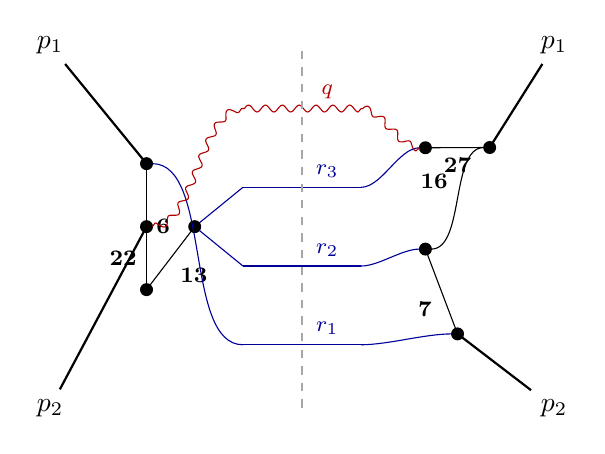
\begin{tikzpicture}
\begin{feynman}
\vertex (Lp1) at (-3.200,2.300) {$p_1$};
\vertex (Lp2) at (-3.200,-2.300) {$p_2$};
\vertex (Lcr1) at (-0.750,-1.500);
\vertex (Lcr2) at (-0.750,-0.500);
\vertex (Lcr3) at (-0.750,0.500);
\vertex (Lcq) at (-0.750,1.500);
\vertex[dot] (L6) at (-1.975,0.800) {};
\vertex[dot] (L22) at (-1.975,-0.800) {};
\vertex[dot] (L13) at (-1.363,0.000) {};
\vertex[dot] (Lroot) at (-1.975,0.000) {};
\vertex (Rp1) at (3.200,2.300) {$p_1$};
\vertex (Rp2) at (3.200,-2.300) {$p_2$};
\vertex (Rcr1) at (0.750,-1.500);
\vertex (Rcr2) at (0.750,-0.500);
\vertex (Rcr3) at (0.750,0.500);
\vertex (Rcq) at (0.750,1.500);
\vertex[dot] (R7) at (1.975,-1.362) {};
\vertex[dot] (R16) at (1.567,-0.285) {};
\vertex[dot] (R27) at (2.383,1.005) {};
\vertex[dot] (Rroot) at (1.567,1.002) {};
\diagram* {
(L6) -- [plain, edge label={\footnotesize\bfseries 6}] (L22),
(L13) -- [plain, edge label={\footnotesize\bfseries 13}] (L22),
(L22) -- [plain, edge label={\footnotesize\bfseries 22}] (Lroot),
(Lp1) -- [plain, thick] (L6),
(Lp2) -- [plain, thick] (Lroot),
(Lcr1) -- [plain, blue!60!black, out=180, in=0, looseness=0.75] (L6),
(Lcr2) -- [plain, blue!60!black] (L13),
(Lcr3) -- [plain, blue!60!black] (L13),
(Lcq) -- [boson, red!70!black, out=180, in=0, looseness=0.75] (Lroot),
(R7) -- [plain, edge label={\footnotesize\bfseries 7}] (R16),
(R16) -- [plain, out=0, in=180, looseness=0.75, edge label={\footnotesize\bfseries 16}] (R27),
(R27) -- [plain, edge label={\footnotesize\bfseries 27}] (Rroot),
(Rp1) -- [plain, thick] (R27),
(Rp2) -- [plain, thick] (R7),
(Rcr1) -- [plain, blue!60!black, out=0, in=180, looseness=0.75] (R7),
(Rcr2) -- [plain, blue!60!black, out=0, in=180, looseness=0.75] (R16),
(Rcr3) -- [plain, blue!60!black, out=0, in=180, looseness=0.75] (Rroot),
(Rcq) -- [boson, red!70!black, out=0, in=180, looseness=0.75] (Rroot),
(Lcr1) -- [plain, blue!60!black] (Rcr1),
(Lcr2) -- [plain, blue!60!black] (Rcr2),
(Lcr3) -- [plain, blue!60!black] (Rcr3),
(Lcq) -- [boson, red!70!black] (Rcq),
};
\end{feynman}
\draw[dashed, gray!70] (0,-2.30) -- (0,2.30);
\node[font=\footnotesize, blue!60!black, above] at (0.32,-1.50) {$r_1$};
\node[font=\footnotesize, blue!60!black, above] at (0.32,-0.50) {$r_2$};
\node[font=\footnotesize, blue!60!black, above] at (0.32,0.50) {$r_3$};
\node[font=\footnotesize, red!70!black, above] at (0.32,1.50) {$q$};
\end{tikzpicture}}\\[2mm]\textbf{FAM[175]} (topo175)\\[2pt]{\footnotesize\begin{tabular}{@{}r@{\ \ }l@{\ \ }l@{}}\textbf{6} & $(p_1+r_1)^2$ & amplitude\\
\textbf{13} & $(r_2+r_3)^2$ & amplitude\\
\textbf{22} & $(p_1+r_1+r_2+r_3)^2$ & amplitude\\
\textbf{7} & $(p_2+r_1)^2$ & conjugate\\
\textbf{16} & $(p_2+r_1+r_2)^2$ & conjugate\\
\textbf{27} & $(p_1+p_2+r_1+r_2)^2$ & conjugate\\\end{tabular}}\\[2pt]{\scriptsize irreducible numerators: 15 = $(p_1+r_1+r_2)^2$}\end{minipage}

\bigskip

\begin{minipage}[t]{0.48\textwidth}\centering\resizebox{0.9\linewidth}{!}{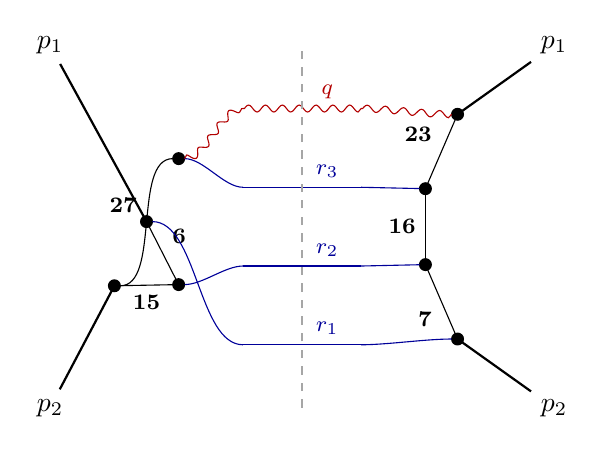
\begin{tikzpicture}
\begin{feynman}
\vertex (Lp1) at (-3.200,2.300) {$p_1$};
\vertex (Lp2) at (-3.200,-2.300) {$p_2$};
\vertex (Lcr1) at (-0.750,-1.500);
\vertex (Lcr2) at (-0.750,-0.500);
\vertex (Lcr3) at (-0.750,0.500);
\vertex (Lcq) at (-0.750,1.500);
\vertex[dot] (L6) at (-1.975,0.064) {};
\vertex[dot] (L15) at (-1.567,-0.736) {};
\vertex[dot] (L27) at (-2.383,-0.751) {};
\vertex[dot] (Lroot) at (-1.567,0.864) {};
\vertex (Rp1) at (3.200,2.300) {$p_1$};
\vertex (Rp2) at (3.200,-2.300) {$p_2$};
\vertex (Rcr1) at (0.750,-1.500);
\vertex (Rcr2) at (0.750,-0.500);
\vertex (Rcr3) at (0.750,0.500);
\vertex (Rcq) at (0.750,1.500);
\vertex[dot] (R7) at (1.975,-1.427) {};
\vertex[dot] (R16) at (1.567,-0.482) {};
\vertex[dot] (R23) at (1.567,0.482) {};
\vertex[dot] (Rroot) at (1.975,1.427) {};
\diagram* {
(L6) -- [plain, edge label={\footnotesize\bfseries 6}] (L15),
(L15) -- [plain, edge label={\footnotesize\bfseries 15}] (L27),
(L27) -- [plain, out=0, in=180, looseness=0.75, edge label={\footnotesize\bfseries 27}] (Lroot),
(Lp1) -- [plain, thick] (L6),
(Lp2) -- [plain, thick] (L27),
(Lcr1) -- [plain, blue!60!black, out=180, in=0, looseness=0.75] (L6),
(Lcr2) -- [plain, blue!60!black, out=180, in=0, looseness=0.75] (L15),
(Lcr3) -- [plain, blue!60!black, out=180, in=0, looseness=0.75] (Lroot),
(Lcq) -- [boson, red!70!black, out=180, in=0, looseness=0.75] (Lroot),
(R7) -- [plain, edge label={\footnotesize\bfseries 7}] (R16),
(R16) -- [plain, edge label={\footnotesize\bfseries 16}] (R23),
(R23) -- [plain, edge label={\footnotesize\bfseries 23}] (Rroot),
(Rp1) -- [plain, thick] (Rroot),
(Rp2) -- [plain, thick] (R7),
(Rcr1) -- [plain, blue!60!black, out=0, in=180, looseness=0.75] (R7),
(Rcr2) -- [plain, blue!60!black] (R16),
(Rcr3) -- [plain, blue!60!black] (R23),
(Rcq) -- [boson, red!70!black, out=0, in=180, looseness=0.75] (Rroot),
(Lcr1) -- [plain, blue!60!black] (Rcr1),
(Lcr2) -- [plain, blue!60!black] (Rcr2),
(Lcr3) -- [plain, blue!60!black] (Rcr3),
(Lcq) -- [boson, red!70!black] (Rcq),
};
\end{feynman}
\draw[dashed, gray!70] (0,-2.30) -- (0,2.30);
\node[font=\footnotesize, blue!60!black, above] at (0.32,-1.50) {$r_1$};
\node[font=\footnotesize, blue!60!black, above] at (0.32,-0.50) {$r_2$};
\node[font=\footnotesize, blue!60!black, above] at (0.32,0.50) {$r_3$};
\node[font=\footnotesize, red!70!black, above] at (0.32,1.50) {$q$};
\end{tikzpicture}}\\[2mm]\textbf{FAM[181]} (topo181)\\[2pt]{\footnotesize\begin{tabular}{@{}r@{\ \ }l@{\ \ }l@{}}\textbf{6} & $(p_1+r_1)^2$ & amplitude\\
\textbf{15} & $(p_1+r_1+r_2)^2$ & amplitude\\
\textbf{27} & $(p_1+p_2+r_1+r_2)^2$ & amplitude\\
\textbf{7} & $(p_2+r_1)^2$ & conjugate\\
\textbf{16} & $(p_2+r_1+r_2)^2$ & conjugate\\
\textbf{23} & $(p_2+r_1+r_2+r_3)^2$ & conjugate\\\end{tabular}}\\[2pt]{\scriptsize irreducible numerators: 18 = $(p_2+r_1+r_3)^2$}\end{minipage}\hfill%
\begin{minipage}[t]{0.48\textwidth}\centering\resizebox{0.9\linewidth}{!}{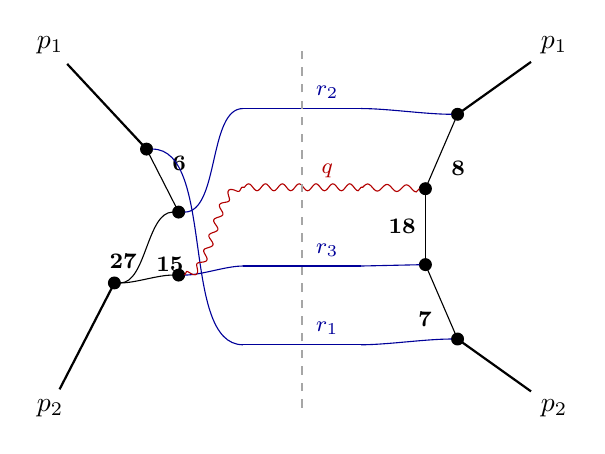
\begin{tikzpicture}
\begin{feynman}
\vertex (Lp1) at (-3.200,2.300) {$p_1$};
\vertex (Lp2) at (-3.200,-2.300) {$p_2$};
\vertex (Lcr1) at (-0.750,-1.500);
\vertex (Lcr2) at (-0.750,1.500);
\vertex (Lcr3) at (-0.750,-0.500);
\vertex (Lcq) at (-0.750,0.500);
\vertex[dot] (L6) at (-1.975,0.985) {};
\vertex[dot] (L15) at (-1.567,0.185) {};
\vertex[dot] (L27) at (-2.383,-0.715) {};
\vertex[dot] (Lroot) at (-1.567,-0.615) {};
\vertex (Rp1) at (3.200,2.300) {$p_1$};
\vertex (Rp2) at (3.200,-2.300) {$p_2$};
\vertex (Rcr1) at (0.750,-1.500);
\vertex (Rcr2) at (0.750,1.500);
\vertex (Rcr3) at (0.750,-0.500);
\vertex (Rcq) at (0.750,0.500);
\vertex[dot] (R7) at (1.975,-1.427) {};
\vertex[dot] (R18) at (1.567,-0.482) {};
\vertex[dot] (R8) at (1.975,1.427) {};
\vertex[dot] (Rroot) at (1.567,0.482) {};
\diagram* {
(L6) -- [plain, edge label={\footnotesize\bfseries 6}] (L15),
(L15) -- [plain, out=180, in=0, looseness=0.75, edge label={\footnotesize\bfseries 15}] (L27),
(L27) -- [plain, out=0, in=180, looseness=0.75, edge label={\footnotesize\bfseries 27}] (Lroot),
(Lp1) -- [plain, thick] (L6),
(Lp2) -- [plain, thick] (L27),
(Lcr1) -- [plain, blue!60!black, out=180, in=0, looseness=0.75] (L6),
(Lcr2) -- [plain, blue!60!black, out=180, in=0, looseness=0.75] (L15),
(Lcr3) -- [plain, blue!60!black, out=180, in=0, looseness=0.75] (Lroot),
(Lcq) -- [boson, red!70!black, out=180, in=0, looseness=0.75] (Lroot),
(R7) -- [plain, edge label={\footnotesize\bfseries 7}] (R18),
(R8) -- [plain, edge label={\footnotesize\bfseries 8}] (Rroot),
(R18) -- [plain, edge label={\footnotesize\bfseries 18}] (Rroot),
(Rp1) -- [plain, thick] (R8),
(Rp2) -- [plain, thick] (R7),
(Rcr1) -- [plain, blue!60!black, out=0, in=180, looseness=0.75] (R7),
(Rcr2) -- [plain, blue!60!black, out=0, in=180, looseness=0.75] (R8),
(Rcr3) -- [plain, blue!60!black] (R18),
(Rcq) -- [boson, red!70!black] (Rroot),
(Lcr1) -- [plain, blue!60!black] (Rcr1),
(Lcr2) -- [plain, blue!60!black] (Rcr2),
(Lcr3) -- [plain, blue!60!black] (Rcr3),
(Lcq) -- [boson, red!70!black] (Rcq),
};
\end{feynman}
\draw[dashed, gray!70] (0,-2.30) -- (0,2.30);
\node[font=\footnotesize, blue!60!black, above] at (0.32,-1.50) {$r_1$};
\node[font=\footnotesize, blue!60!black, above] at (0.32,1.50) {$r_2$};
\node[font=\footnotesize, blue!60!black, above] at (0.32,-0.50) {$r_3$};
\node[font=\footnotesize, red!70!black, above] at (0.32,0.50) {$q$};
\end{tikzpicture}}\\[2mm]\textbf{FAM[187]} (topo187)\\[2pt]{\footnotesize\begin{tabular}{@{}r@{\ \ }l@{\ \ }l@{}}\textbf{6} & $(p_1+r_1)^2$ & amplitude\\
\textbf{15} & $(p_1+r_1+r_2)^2$ & amplitude\\
\textbf{27} & $(p_1+p_2+r_1+r_2)^2$ & amplitude\\
\textbf{7} & $(p_2+r_1)^2$ & conjugate\\
\textbf{8} & $(p_1+r_2)^2$ & conjugate\\
\textbf{18} & $(p_2+r_1+r_3)^2$ & conjugate\\\end{tabular}}\\[2pt]{\scriptsize irreducible numerators: 28 = $(p_1+p_2+r_1+r_3)^2$}\end{minipage}

\bigskip

\begin{minipage}[t]{0.48\textwidth}\centering\resizebox{0.9\linewidth}{!}{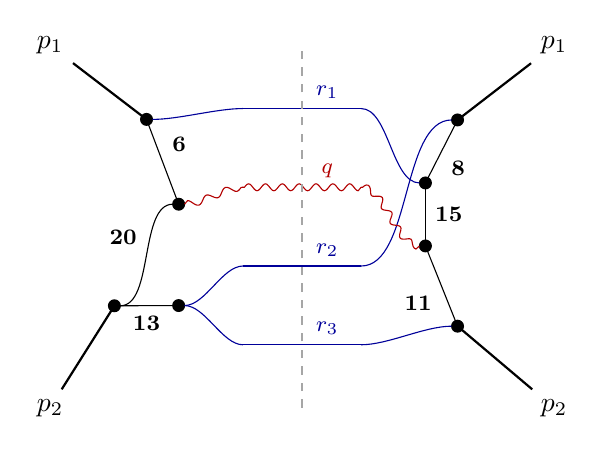
\begin{tikzpicture}
\begin{feynman}
\vertex (Lp1) at (-3.200,2.300) {$p_1$};
\vertex (Lp2) at (-3.200,-2.300) {$p_2$};
\vertex (Lcr1) at (-0.750,1.500);
\vertex (Lcr2) at (-0.750,-0.500);
\vertex (Lcr3) at (-0.750,-1.500);
\vertex (Lcq) at (-0.750,0.500);
\vertex[dot] (L6) at (-1.975,1.362) {};
\vertex[dot] (Lroot) at (-1.567,0.285) {};
\vertex[dot] (L13) at (-1.567,-1.002) {};
\vertex[dot] (L20) at (-2.383,-1.005) {};
\vertex (Rp1) at (3.200,2.300) {$p_1$};
\vertex (Rp2) at (3.200,-2.300) {$p_2$};
\vertex (Rcr1) at (0.750,1.500);
\vertex (Rcr2) at (0.750,-0.500);
\vertex (Rcr3) at (0.750,-1.500);
\vertex (Rcq) at (0.750,0.500);
\vertex[dot] (R8) at (1.975,1.355) {};
\vertex[dot] (R15) at (1.567,0.555) {};
\vertex[dot] (R11) at (1.975,-1.264) {};
\vertex[dot] (Rroot) at (1.567,-0.245) {};
\diagram* {
(L6) -- [plain, edge label={\footnotesize\bfseries 6}] (Lroot),
(L13) -- [plain, edge label={\footnotesize\bfseries 13}] (L20),
(L20) -- [plain, out=0, in=180, looseness=0.75, edge label={\footnotesize\bfseries 20}] (Lroot),
(Lp1) -- [plain, thick] (L6),
(Lp2) -- [plain, thick] (L20),
(Lcr1) -- [plain, blue!60!black, out=180, in=0, looseness=0.75] (L6),
(Lcr2) -- [plain, blue!60!black, out=180, in=0, looseness=0.75] (L13),
(Lcr3) -- [plain, blue!60!black, out=180, in=0, looseness=0.75] (L13),
(Lcq) -- [boson, red!70!black, out=180, in=0, looseness=0.75] (Lroot),
(R8) -- [plain, edge label={\footnotesize\bfseries 8}] (R15),
(R11) -- [plain, edge label={\footnotesize\bfseries 11}] (Rroot),
(R15) -- [plain, edge label={\footnotesize\bfseries 15}] (Rroot),
(Rp1) -- [plain, thick] (R8),
(Rp2) -- [plain, thick] (R11),
(Rcr1) -- [plain, blue!60!black, out=0, in=180, looseness=0.75] (R15),
(Rcr2) -- [plain, blue!60!black, out=0, in=180, looseness=0.75] (R8),
(Rcr3) -- [plain, blue!60!black, out=0, in=180, looseness=0.75] (R11),
(Rcq) -- [boson, red!70!black, out=0, in=180, looseness=0.75] (Rroot),
(Lcr1) -- [plain, blue!60!black] (Rcr1),
(Lcr2) -- [plain, blue!60!black] (Rcr2),
(Lcr3) -- [plain, blue!60!black] (Rcr3),
(Lcq) -- [boson, red!70!black] (Rcq),
};
\end{feynman}
\draw[dashed, gray!70] (0,-2.30) -- (0,2.30);
\node[font=\footnotesize, blue!60!black, above] at (0.32,1.50) {$r_1$};
\node[font=\footnotesize, blue!60!black, above] at (0.32,-0.50) {$r_2$};
\node[font=\footnotesize, blue!60!black, above] at (0.32,-1.50) {$r_3$};
\node[font=\footnotesize, red!70!black, above] at (0.32,0.50) {$q$};
\end{tikzpicture}}\\[2mm]\textbf{FAM[193]} (topo193)\\[2pt]{\footnotesize\begin{tabular}{@{}r@{\ \ }l@{\ \ }l@{}}\textbf{6} & $(p_1+r_1)^2$ & amplitude\\
\textbf{13} & $(r_2+r_3)^2$ & amplitude\\
\textbf{20} & $(p_2+r_2+r_3)^2$ & amplitude\\
\textbf{8} & $(p_1+r_2)^2$ & conjugate\\
\textbf{11} & $(p_2+r_3)^2$ & conjugate\\
\textbf{15} & $(p_1+r_1+r_2)^2$ & conjugate\\\end{tabular}}\\[2pt]{\scriptsize irreducible numerators: 21 = $(r_1+r_2+r_3)^2$}\end{minipage}\hfill%
\begin{minipage}[t]{0.48\textwidth}\centering\resizebox{0.9\linewidth}{!}{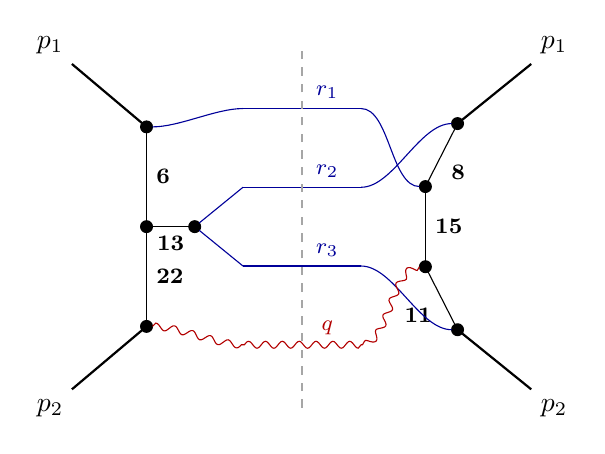
\begin{tikzpicture}
\begin{feynman}
\vertex (Lp1) at (-3.200,2.300) {$p_1$};
\vertex (Lp2) at (-3.200,-2.300) {$p_2$};
\vertex (Lcr1) at (-0.750,1.500);
\vertex (Lcr2) at (-0.750,0.500);
\vertex (Lcr3) at (-0.750,-0.500);
\vertex (Lcq) at (-0.750,-1.500);
\vertex[dot] (L6) at (-1.975,1.267) {};
\vertex[dot] (L22) at (-1.975,0.000) {};
\vertex[dot] (L13) at (-1.363,0.000) {};
\vertex[dot] (Lroot) at (-1.975,-1.267) {};
\vertex (Rp1) at (3.200,2.300) {$p_1$};
\vertex (Rp2) at (3.200,-2.300) {$p_2$};
\vertex (Rcr1) at (0.750,1.500);
\vertex (Rcr2) at (0.750,0.500);
\vertex (Rcr3) at (0.750,-0.500);
\vertex (Rcq) at (0.750,-1.500);
\vertex[dot] (R8) at (1.975,1.309) {};
\vertex[dot] (R15) at (1.567,0.509) {};
\vertex[dot] (R11) at (1.975,-1.309) {};
\vertex[dot] (Rroot) at (1.567,-0.509) {};
\diagram* {
(L6) -- [plain, edge label={\footnotesize\bfseries 6}] (L22),
(L13) -- [plain, edge label={\footnotesize\bfseries 13}] (L22),
(L22) -- [plain, edge label={\footnotesize\bfseries 22}] (Lroot),
(Lp1) -- [plain, thick] (L6),
(Lp2) -- [plain, thick] (Lroot),
(Lcr1) -- [plain, blue!60!black, out=180, in=0, looseness=0.75] (L6),
(Lcr2) -- [plain, blue!60!black] (L13),
(Lcr3) -- [plain, blue!60!black] (L13),
(Lcq) -- [boson, red!70!black, out=180, in=0, looseness=0.75] (Lroot),
(R8) -- [plain, edge label={\footnotesize\bfseries 8}] (R15),
(R11) -- [plain, edge label={\footnotesize\bfseries 11}] (Rroot),
(R15) -- [plain, edge label={\footnotesize\bfseries 15}] (Rroot),
(Rp1) -- [plain, thick] (R8),
(Rp2) -- [plain, thick] (R11),
(Rcr1) -- [plain, blue!60!black, out=0, in=180, looseness=0.75] (R15),
(Rcr2) -- [plain, blue!60!black, out=0, in=180, looseness=0.75] (R8),
(Rcr3) -- [plain, blue!60!black, out=0, in=180, looseness=0.75] (R11),
(Rcq) -- [boson, red!70!black, out=0, in=180, looseness=0.75] (Rroot),
(Lcr1) -- [plain, blue!60!black] (Rcr1),
(Lcr2) -- [plain, blue!60!black] (Rcr2),
(Lcr3) -- [plain, blue!60!black] (Rcr3),
(Lcq) -- [boson, red!70!black] (Rcq),
};
\end{feynman}
\draw[dashed, gray!70] (0,-2.30) -- (0,2.30);
\node[font=\footnotesize, blue!60!black, above] at (0.32,1.50) {$r_1$};
\node[font=\footnotesize, blue!60!black, above] at (0.32,0.50) {$r_2$};
\node[font=\footnotesize, blue!60!black, above] at (0.32,-0.50) {$r_3$};
\node[font=\footnotesize, red!70!black, above] at (0.32,-1.50) {$q$};
\end{tikzpicture}}\\[2mm]\textbf{FAM[199]} (topo199)\\[2pt]{\footnotesize\begin{tabular}{@{}r@{\ \ }l@{\ \ }l@{}}\textbf{6} & $(p_1+r_1)^2$ & amplitude\\
\textbf{13} & $(r_2+r_3)^2$ & amplitude\\
\textbf{22} & $(p_1+r_1+r_2+r_3)^2$ & amplitude\\
\textbf{8} & $(p_1+r_2)^2$ & conjugate\\
\textbf{11} & $(p_2+r_3)^2$ & conjugate\\
\textbf{15} & $(p_1+r_1+r_2)^2$ & conjugate\\\end{tabular}}\\[2pt]{\scriptsize irreducible numerators: 29 = $(p_1+p_2+r_2+r_3)^2$}\end{minipage}

\bigskip

\begin{minipage}[t]{0.48\textwidth}\centering\resizebox{0.9\linewidth}{!}{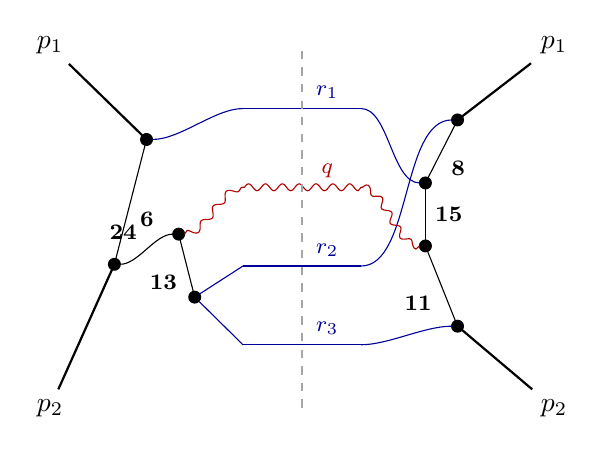
\begin{tikzpicture}
\begin{feynman}
\vertex (Lp1) at (-3.200,2.300) {$p_1$};
\vertex (Lp2) at (-3.200,-2.300) {$p_2$};
\vertex (Lcr1) at (-0.750,1.500);
\vertex (Lcr2) at (-0.750,-0.500);
\vertex (Lcr3) at (-0.750,-1.500);
\vertex (Lcq) at (-0.750,0.500);
\vertex[dot] (L6) at (-1.975,1.107) {};
\vertex[dot] (L24) at (-2.383,-0.478) {};
\vertex[dot] (L13) at (-1.363,-0.895) {};
\vertex[dot] (Lroot) at (-1.567,-0.095) {};
\vertex (Rp1) at (3.200,2.300) {$p_1$};
\vertex (Rp2) at (3.200,-2.300) {$p_2$};
\vertex (Rcr1) at (0.750,1.500);
\vertex (Rcr2) at (0.750,-0.500);
\vertex (Rcr3) at (0.750,-1.500);
\vertex (Rcq) at (0.750,0.500);
\vertex[dot] (R8) at (1.975,1.355) {};
\vertex[dot] (R15) at (1.567,0.555) {};
\vertex[dot] (R11) at (1.975,-1.264) {};
\vertex[dot] (Rroot) at (1.567,-0.245) {};
\diagram* {
(L6) -- [plain, edge label={\footnotesize\bfseries 6}] (L24),
(L13) -- [plain, edge label={\footnotesize\bfseries 13}] (Lroot),
(L24) -- [plain, out=0, in=180, looseness=0.75, edge label={\footnotesize\bfseries 24}] (Lroot),
(Lp1) -- [plain, thick] (L6),
(Lp2) -- [plain, thick] (L24),
(Lcr1) -- [plain, blue!60!black, out=180, in=0, looseness=0.75] (L6),
(Lcr2) -- [plain, blue!60!black] (L13),
(Lcr3) -- [plain, blue!60!black] (L13),
(Lcq) -- [boson, red!70!black, out=180, in=0, looseness=0.75] (Lroot),
(R8) -- [plain, edge label={\footnotesize\bfseries 8}] (R15),
(R11) -- [plain, edge label={\footnotesize\bfseries 11}] (Rroot),
(R15) -- [plain, edge label={\footnotesize\bfseries 15}] (Rroot),
(Rp1) -- [plain, thick] (R8),
(Rp2) -- [plain, thick] (R11),
(Rcr1) -- [plain, blue!60!black, out=0, in=180, looseness=0.75] (R15),
(Rcr2) -- [plain, blue!60!black, out=0, in=180, looseness=0.75] (R8),
(Rcr3) -- [plain, blue!60!black, out=0, in=180, looseness=0.75] (R11),
(Rcq) -- [boson, red!70!black, out=0, in=180, looseness=0.75] (Rroot),
(Lcr1) -- [plain, blue!60!black] (Rcr1),
(Lcr2) -- [plain, blue!60!black] (Rcr2),
(Lcr3) -- [plain, blue!60!black] (Rcr3),
(Lcq) -- [boson, red!70!black] (Rcq),
};
\end{feynman}
\draw[dashed, gray!70] (0,-2.30) -- (0,2.30);
\node[font=\footnotesize, blue!60!black, above] at (0.32,1.50) {$r_1$};
\node[font=\footnotesize, blue!60!black, above] at (0.32,-0.50) {$r_2$};
\node[font=\footnotesize, blue!60!black, above] at (0.32,-1.50) {$r_3$};
\node[font=\footnotesize, red!70!black, above] at (0.32,0.50) {$q$};
\end{tikzpicture}}\\[2mm]\textbf{FAM[205]} (topo205)\\[2pt]{\footnotesize\begin{tabular}{@{}r@{\ \ }l@{\ \ }l@{}}\textbf{6} & $(p_1+r_1)^2$ & amplitude\\
\textbf{13} & $(r_2+r_3)^2$ & amplitude\\
\textbf{24} & $(p_1+p_2+r_1)^2$ & amplitude\\
\textbf{8} & $(p_1+r_2)^2$ & conjugate\\
\textbf{11} & $(p_2+r_3)^2$ & conjugate\\
\textbf{15} & $(p_1+r_1+r_2)^2$ & conjugate\\\end{tabular}}\\[2pt]{\scriptsize irreducible numerators: 27 = $(p_1+p_2+r_1+r_2)^2$}\end{minipage}\hfill%
\begin{minipage}[t]{0.48\textwidth}\centering\resizebox{0.9\linewidth}{!}{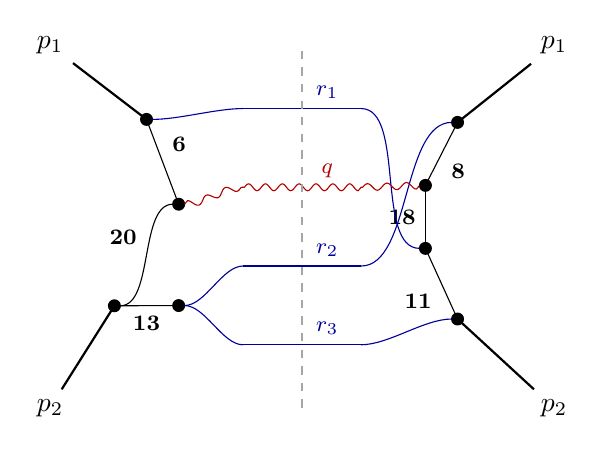
\begin{tikzpicture}
\begin{feynman}
\vertex (Lp1) at (-3.200,2.300) {$p_1$};
\vertex (Lp2) at (-3.200,-2.300) {$p_2$};
\vertex (Lcr1) at (-0.750,1.500);
\vertex (Lcr2) at (-0.750,-0.500);
\vertex (Lcr3) at (-0.750,-1.500);
\vertex (Lcq) at (-0.750,0.500);
\vertex[dot] (L6) at (-1.975,1.362) {};
\vertex[dot] (Lroot) at (-1.567,0.285) {};
\vertex[dot] (L13) at (-1.567,-1.002) {};
\vertex[dot] (L20) at (-2.383,-1.005) {};
\vertex (Rp1) at (3.200,2.300) {$p_1$};
\vertex (Rp2) at (3.200,-2.300) {$p_2$};
\vertex (Rcr1) at (0.750,1.500);
\vertex (Rcr2) at (0.750,-0.500);
\vertex (Rcr3) at (0.750,-1.500);
\vertex (Rcq) at (0.750,0.500);
\vertex[dot] (R8) at (1.975,1.324) {};
\vertex[dot] (Rroot) at (1.567,0.524) {};
\vertex[dot] (R11) at (1.975,-1.173) {};
\vertex[dot] (R18) at (1.567,-0.276) {};
\diagram* {
(L6) -- [plain, edge label={\footnotesize\bfseries 6}] (Lroot),
(L13) -- [plain, edge label={\footnotesize\bfseries 13}] (L20),
(L20) -- [plain, out=0, in=180, looseness=0.75, edge label={\footnotesize\bfseries 20}] (Lroot),
(Lp1) -- [plain, thick] (L6),
(Lp2) -- [plain, thick] (L20),
(Lcr1) -- [plain, blue!60!black, out=180, in=0, looseness=0.75] (L6),
(Lcr2) -- [plain, blue!60!black, out=180, in=0, looseness=0.75] (L13),
(Lcr3) -- [plain, blue!60!black, out=180, in=0, looseness=0.75] (L13),
(Lcq) -- [boson, red!70!black, out=180, in=0, looseness=0.75] (Lroot),
(R8) -- [plain, edge label={\footnotesize\bfseries 8}] (Rroot),
(R11) -- [plain, edge label={\footnotesize\bfseries 11}] (R18),
(R18) -- [plain, edge label={\footnotesize\bfseries 18}] (Rroot),
(Rp1) -- [plain, thick] (R8),
(Rp2) -- [plain, thick] (R11),
(Rcr1) -- [plain, blue!60!black, out=0, in=180, looseness=0.75] (R18),
(Rcr2) -- [plain, blue!60!black, out=0, in=180, looseness=0.75] (R8),
(Rcr3) -- [plain, blue!60!black, out=0, in=180, looseness=0.75] (R11),
(Rcq) -- [boson, red!70!black] (Rroot),
(Lcr1) -- [plain, blue!60!black] (Rcr1),
(Lcr2) -- [plain, blue!60!black] (Rcr2),
(Lcr3) -- [plain, blue!60!black] (Rcr3),
(Lcq) -- [boson, red!70!black] (Rcq),
};
\end{feynman}
\draw[dashed, gray!70] (0,-2.30) -- (0,2.30);
\node[font=\footnotesize, blue!60!black, above] at (0.32,1.50) {$r_1$};
\node[font=\footnotesize, blue!60!black, above] at (0.32,-0.50) {$r_2$};
\node[font=\footnotesize, blue!60!black, above] at (0.32,-1.50) {$r_3$};
\node[font=\footnotesize, red!70!black, above] at (0.32,0.50) {$q$};
\end{tikzpicture}}\\[2mm]\textbf{FAM[211]} (topo211)\\[2pt]{\footnotesize\begin{tabular}{@{}r@{\ \ }l@{\ \ }l@{}}\textbf{6} & $(p_1+r_1)^2$ & amplitude\\
\textbf{13} & $(r_2+r_3)^2$ & amplitude\\
\textbf{20} & $(p_2+r_2+r_3)^2$ & amplitude\\
\textbf{8} & $(p_1+r_2)^2$ & conjugate\\
\textbf{11} & $(p_2+r_3)^2$ & conjugate\\
\textbf{18} & $(p_2+r_1+r_3)^2$ & conjugate\\\end{tabular}}\\[2pt]{\scriptsize irreducible numerators: 19 = $(p_1+r_2+r_3)^2$}\end{minipage}

\bigskip

\begin{minipage}[t]{0.48\textwidth}\centering\resizebox{0.9\linewidth}{!}{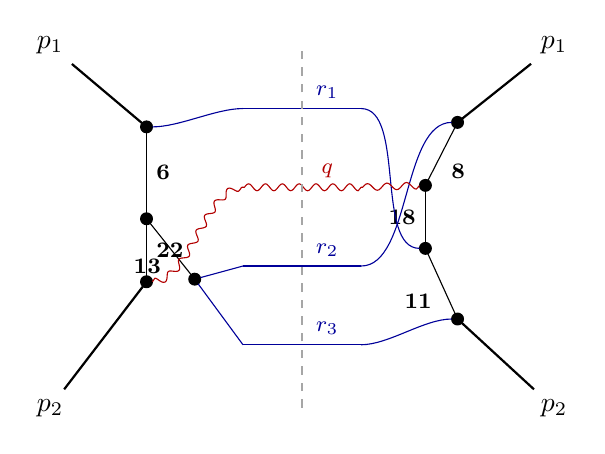
\begin{tikzpicture}
\begin{feynman}
\vertex (Lp1) at (-3.200,2.300) {$p_1$};
\vertex (Lp2) at (-3.200,-2.300) {$p_2$};
\vertex (Lcr1) at (-0.750,1.500);
\vertex (Lcr2) at (-0.750,-0.500);
\vertex (Lcr3) at (-0.750,-1.500);
\vertex (Lcq) at (-0.750,0.500);
\vertex[dot] (L6) at (-1.975,1.267) {};
\vertex[dot] (L22) at (-1.975,0.100) {};
\vertex[dot] (L13) at (-1.363,-0.667) {};
\vertex[dot] (Lroot) at (-1.975,-0.700) {};
\vertex (Rp1) at (3.200,2.300) {$p_1$};
\vertex (Rp2) at (3.200,-2.300) {$p_2$};
\vertex (Rcr1) at (0.750,1.500);
\vertex (Rcr2) at (0.750,-0.500);
\vertex (Rcr3) at (0.750,-1.500);
\vertex (Rcq) at (0.750,0.500);
\vertex[dot] (R8) at (1.975,1.324) {};
\vertex[dot] (Rroot) at (1.567,0.524) {};
\vertex[dot] (R11) at (1.975,-1.173) {};
\vertex[dot] (R18) at (1.567,-0.276) {};
\diagram* {
(L6) -- [plain, edge label={\footnotesize\bfseries 6}] (L22),
(L13) -- [plain, edge label={\footnotesize\bfseries 13}] (L22),
(L22) -- [plain, edge label={\footnotesize\bfseries 22}] (Lroot),
(Lp1) -- [plain, thick] (L6),
(Lp2) -- [plain, thick] (Lroot),
(Lcr1) -- [plain, blue!60!black, out=180, in=0, looseness=0.75] (L6),
(Lcr2) -- [plain, blue!60!black] (L13),
(Lcr3) -- [plain, blue!60!black] (L13),
(Lcq) -- [boson, red!70!black, out=180, in=0, looseness=0.75] (Lroot),
(R8) -- [plain, edge label={\footnotesize\bfseries 8}] (Rroot),
(R11) -- [plain, edge label={\footnotesize\bfseries 11}] (R18),
(R18) -- [plain, edge label={\footnotesize\bfseries 18}] (Rroot),
(Rp1) -- [plain, thick] (R8),
(Rp2) -- [plain, thick] (R11),
(Rcr1) -- [plain, blue!60!black, out=0, in=180, looseness=0.75] (R18),
(Rcr2) -- [plain, blue!60!black, out=0, in=180, looseness=0.75] (R8),
(Rcr3) -- [plain, blue!60!black, out=0, in=180, looseness=0.75] (R11),
(Rcq) -- [boson, red!70!black] (Rroot),
(Lcr1) -- [plain, blue!60!black] (Rcr1),
(Lcr2) -- [plain, blue!60!black] (Rcr2),
(Lcr3) -- [plain, blue!60!black] (Rcr3),
(Lcq) -- [boson, red!70!black] (Rcq),
};
\end{feynman}
\draw[dashed, gray!70] (0,-2.30) -- (0,2.30);
\node[font=\footnotesize, blue!60!black, above] at (0.32,1.50) {$r_1$};
\node[font=\footnotesize, blue!60!black, above] at (0.32,-0.50) {$r_2$};
\node[font=\footnotesize, blue!60!black, above] at (0.32,-1.50) {$r_3$};
\node[font=\footnotesize, red!70!black, above] at (0.32,0.50) {$q$};
\end{tikzpicture}}\\[2mm]\textbf{FAM[217]} (topo217)\\[2pt]{\footnotesize\begin{tabular}{@{}r@{\ \ }l@{\ \ }l@{}}\textbf{6} & $(p_1+r_1)^2$ & amplitude\\
\textbf{13} & $(r_2+r_3)^2$ & amplitude\\
\textbf{22} & $(p_1+r_1+r_2+r_3)^2$ & amplitude\\
\textbf{8} & $(p_1+r_2)^2$ & conjugate\\
\textbf{11} & $(p_2+r_3)^2$ & conjugate\\
\textbf{18} & $(p_2+r_1+r_3)^2$ & conjugate\\\end{tabular}}\\[2pt]{\scriptsize irreducible numerators: 17 = $(p_1+r_1+r_3)^2$}\end{minipage}\hfill%
\begin{minipage}[t]{0.48\textwidth}\centering\resizebox{0.9\linewidth}{!}{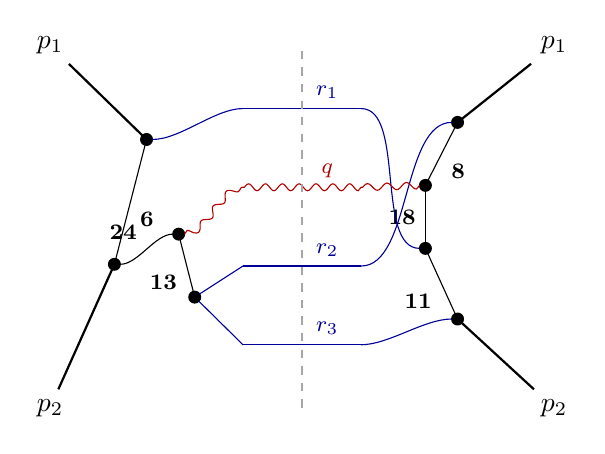
\begin{tikzpicture}
\begin{feynman}
\vertex (Lp1) at (-3.200,2.300) {$p_1$};
\vertex (Lp2) at (-3.200,-2.300) {$p_2$};
\vertex (Lcr1) at (-0.750,1.500);
\vertex (Lcr2) at (-0.750,-0.500);
\vertex (Lcr3) at (-0.750,-1.500);
\vertex (Lcq) at (-0.750,0.500);
\vertex[dot] (L6) at (-1.975,1.107) {};
\vertex[dot] (L24) at (-2.383,-0.478) {};
\vertex[dot] (L13) at (-1.363,-0.895) {};
\vertex[dot] (Lroot) at (-1.567,-0.095) {};
\vertex (Rp1) at (3.200,2.300) {$p_1$};
\vertex (Rp2) at (3.200,-2.300) {$p_2$};
\vertex (Rcr1) at (0.750,1.500);
\vertex (Rcr2) at (0.750,-0.500);
\vertex (Rcr3) at (0.750,-1.500);
\vertex (Rcq) at (0.750,0.500);
\vertex[dot] (R8) at (1.975,1.324) {};
\vertex[dot] (Rroot) at (1.567,0.524) {};
\vertex[dot] (R11) at (1.975,-1.173) {};
\vertex[dot] (R18) at (1.567,-0.276) {};
\diagram* {
(L6) -- [plain, edge label={\footnotesize\bfseries 6}] (L24),
(L13) -- [plain, edge label={\footnotesize\bfseries 13}] (Lroot),
(L24) -- [plain, out=0, in=180, looseness=0.75, edge label={\footnotesize\bfseries 24}] (Lroot),
(Lp1) -- [plain, thick] (L6),
(Lp2) -- [plain, thick] (L24),
(Lcr1) -- [plain, blue!60!black, out=180, in=0, looseness=0.75] (L6),
(Lcr2) -- [plain, blue!60!black] (L13),
(Lcr3) -- [plain, blue!60!black] (L13),
(Lcq) -- [boson, red!70!black, out=180, in=0, looseness=0.75] (Lroot),
(R8) -- [plain, edge label={\footnotesize\bfseries 8}] (Rroot),
(R11) -- [plain, edge label={\footnotesize\bfseries 11}] (R18),
(R18) -- [plain, edge label={\footnotesize\bfseries 18}] (Rroot),
(Rp1) -- [plain, thick] (R8),
(Rp2) -- [plain, thick] (R11),
(Rcr1) -- [plain, blue!60!black, out=0, in=180, looseness=0.75] (R18),
(Rcr2) -- [plain, blue!60!black, out=0, in=180, looseness=0.75] (R8),
(Rcr3) -- [plain, blue!60!black, out=0, in=180, looseness=0.75] (R11),
(Rcq) -- [boson, red!70!black] (Rroot),
(Lcr1) -- [plain, blue!60!black] (Rcr1),
(Lcr2) -- [plain, blue!60!black] (Rcr2),
(Lcr3) -- [plain, blue!60!black] (Rcr3),
(Lcq) -- [boson, red!70!black] (Rcq),
};
\end{feynman}
\draw[dashed, gray!70] (0,-2.30) -- (0,2.30);
\node[font=\footnotesize, blue!60!black, above] at (0.32,1.50) {$r_1$};
\node[font=\footnotesize, blue!60!black, above] at (0.32,-0.50) {$r_2$};
\node[font=\footnotesize, blue!60!black, above] at (0.32,-1.50) {$r_3$};
\node[font=\footnotesize, red!70!black, above] at (0.32,0.50) {$q$};
\end{tikzpicture}}\\[2mm]\textbf{FAM[223]} (topo223)\\[2pt]{\footnotesize\begin{tabular}{@{}r@{\ \ }l@{\ \ }l@{}}\textbf{6} & $(p_1+r_1)^2$ & amplitude\\
\textbf{13} & $(r_2+r_3)^2$ & amplitude\\
\textbf{24} & $(p_1+p_2+r_1)^2$ & amplitude\\
\textbf{8} & $(p_1+r_2)^2$ & conjugate\\
\textbf{11} & $(p_2+r_3)^2$ & conjugate\\
\textbf{18} & $(p_2+r_1+r_3)^2$ & conjugate\\\end{tabular}}\\[2pt]{\scriptsize irreducible numerators: 28 = $(p_1+p_2+r_1+r_3)^2$}\end{minipage}

\bigskip

\begin{minipage}[t]{0.48\textwidth}\centering\resizebox{0.9\linewidth}{!}{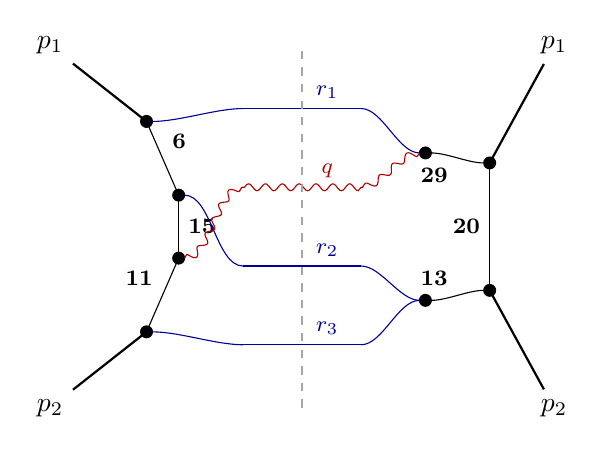
\begin{tikzpicture}
\begin{feynman}
\vertex (Lp1) at (-3.200,2.300) {$p_1$};
\vertex (Lp2) at (-3.200,-2.300) {$p_2$};
\vertex (Lcr1) at (-0.750,1.500);
\vertex (Lcr2) at (-0.750,-0.500);
\vertex (Lcr3) at (-0.750,-1.500);
\vertex (Lcq) at (-0.750,0.500);
\vertex[dot] (L6) at (-1.975,1.336) {};
\vertex[dot] (L15) at (-1.567,0.400) {};
\vertex[dot] (L11) at (-1.975,-1.336) {};
\vertex[dot] (Lroot) at (-1.567,-0.400) {};
\vertex (Rp1) at (3.200,2.300) {$p_1$};
\vertex (Rp2) at (3.200,-2.300) {$p_2$};
\vertex (Rcr1) at (0.750,1.500);
\vertex (Rcr2) at (0.750,-0.500);
\vertex (Rcr3) at (0.750,-1.500);
\vertex (Rcq) at (0.750,0.500);
\vertex[dot] (R13) at (1.567,-0.936) {};
\vertex[dot] (R20) at (2.383,-0.809) {};
\vertex[dot] (R29) at (2.383,0.809) {};
\vertex[dot] (Rroot) at (1.567,0.936) {};
\diagram* {
(L6) -- [plain, edge label={\footnotesize\bfseries 6}] (L15),
(L11) -- [plain, edge label={\footnotesize\bfseries 11}] (Lroot),
(L15) -- [plain, edge label={\footnotesize\bfseries 15}] (Lroot),
(Lp1) -- [plain, thick] (L6),
(Lp2) -- [plain, thick] (L11),
(Lcr1) -- [plain, blue!60!black, out=180, in=0, looseness=0.75] (L6),
(Lcr2) -- [plain, blue!60!black, out=180, in=0, looseness=0.75] (L15),
(Lcr3) -- [plain, blue!60!black, out=180, in=0, looseness=0.75] (L11),
(Lcq) -- [boson, red!70!black, out=180, in=0, looseness=0.75] (Lroot),
(R13) -- [plain, out=0, in=180, looseness=0.75, edge label={\footnotesize\bfseries 13}] (R20),
(R20) -- [plain, edge label={\footnotesize\bfseries 20}] (R29),
(R29) -- [plain, out=180, in=0, looseness=0.75, edge label={\footnotesize\bfseries 29}] (Rroot),
(Rp1) -- [plain, thick] (R29),
(Rp2) -- [plain, thick] (R20),
(Rcr1) -- [plain, blue!60!black, out=0, in=180, looseness=0.75] (Rroot),
(Rcr2) -- [plain, blue!60!black, out=0, in=180, looseness=0.75] (R13),
(Rcr3) -- [plain, blue!60!black, out=0, in=180, looseness=0.75] (R13),
(Rcq) -- [boson, red!70!black, out=0, in=180, looseness=0.75] (Rroot),
(Lcr1) -- [plain, blue!60!black] (Rcr1),
(Lcr2) -- [plain, blue!60!black] (Rcr2),
(Lcr3) -- [plain, blue!60!black] (Rcr3),
(Lcq) -- [boson, red!70!black] (Rcq),
};
\end{feynman}
\draw[dashed, gray!70] (0,-2.30) -- (0,2.30);
\node[font=\footnotesize, blue!60!black, above] at (0.32,1.50) {$r_1$};
\node[font=\footnotesize, blue!60!black, above] at (0.32,-0.50) {$r_2$};
\node[font=\footnotesize, blue!60!black, above] at (0.32,-1.50) {$r_3$};
\node[font=\footnotesize, red!70!black, above] at (0.32,0.50) {$q$};
\end{tikzpicture}}\\[2mm]\textbf{FAM[229]} (topo229)\\[2pt]{\footnotesize\begin{tabular}{@{}r@{\ \ }l@{\ \ }l@{}}\textbf{6} & $(p_1+r_1)^2$ & amplitude\\
\textbf{11} & $(p_2+r_3)^2$ & amplitude\\
\textbf{15} & $(p_1+r_1+r_2)^2$ & amplitude\\
\textbf{13} & $(r_2+r_3)^2$ & conjugate\\
\textbf{20} & $(p_2+r_2+r_3)^2$ & conjugate\\
\textbf{29} & $(p_1+p_2+r_2+r_3)^2$ & conjugate\\\end{tabular}}\\[2pt]{\scriptsize irreducible numerators: 8 = $(p_1+r_2)^2$}\end{minipage}\hfill%
\begin{minipage}[t]{0.48\textwidth}\centering\resizebox{0.9\linewidth}{!}{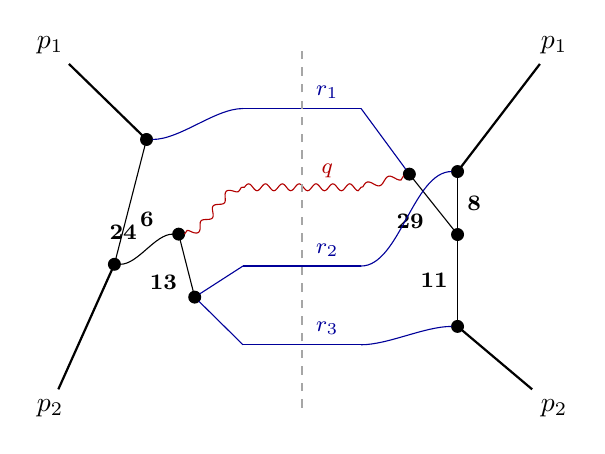
\begin{tikzpicture}
\begin{feynman}
\vertex (Lp1) at (-3.200,2.300) {$p_1$};
\vertex (Lp2) at (-3.200,-2.300) {$p_2$};
\vertex (Lcr1) at (-0.750,1.500);
\vertex (Lcr2) at (-0.750,-0.500);
\vertex (Lcr3) at (-0.750,-1.500);
\vertex (Lcq) at (-0.750,0.500);
\vertex[dot] (L6) at (-1.975,1.107) {};
\vertex[dot] (L24) at (-2.383,-0.478) {};
\vertex[dot] (L13) at (-1.363,-0.895) {};
\vertex[dot] (Lroot) at (-1.567,-0.095) {};
\vertex (Rp1) at (3.200,2.300) {$p_1$};
\vertex (Rp2) at (3.200,-2.300) {$p_2$};
\vertex (Rcr1) at (0.750,1.500);
\vertex (Rcr2) at (0.750,-0.500);
\vertex (Rcr3) at (0.750,-1.500);
\vertex (Rcq) at (0.750,0.500);
\vertex[dot] (R8) at (1.975,0.700) {};
\vertex[dot] (R29) at (1.975,-0.100) {};
\vertex[dot] (R11) at (1.975,-1.267) {};
\vertex[dot] (Rroot) at (1.363,0.667) {};
\diagram* {
(L6) -- [plain, edge label={\footnotesize\bfseries 6}] (L24),
(L13) -- [plain, edge label={\footnotesize\bfseries 13}] (Lroot),
(L24) -- [plain, out=0, in=180, looseness=0.75, edge label={\footnotesize\bfseries 24}] (Lroot),
(Lp1) -- [plain, thick] (L6),
(Lp2) -- [plain, thick] (L24),
(Lcr1) -- [plain, blue!60!black, out=180, in=0, looseness=0.75] (L6),
(Lcr2) -- [plain, blue!60!black] (L13),
(Lcr3) -- [plain, blue!60!black] (L13),
(Lcq) -- [boson, red!70!black, out=180, in=0, looseness=0.75] (Lroot),
(R8) -- [plain, edge label={\footnotesize\bfseries 8}] (R29),
(R11) -- [plain, edge label={\footnotesize\bfseries 11}] (R29),
(R29) -- [plain, edge label={\footnotesize\bfseries 29}] (Rroot),
(Rp1) -- [plain, thick] (R8),
(Rp2) -- [plain, thick] (R11),
(Rcr1) -- [plain, blue!60!black] (Rroot),
(Rcr2) -- [plain, blue!60!black, out=0, in=180, looseness=0.75] (R8),
(Rcr3) -- [plain, blue!60!black, out=0, in=180, looseness=0.75] (R11),
(Rcq) -- [boson, red!70!black] (Rroot),
(Lcr1) -- [plain, blue!60!black] (Rcr1),
(Lcr2) -- [plain, blue!60!black] (Rcr2),
(Lcr3) -- [plain, blue!60!black] (Rcr3),
(Lcq) -- [boson, red!70!black] (Rcq),
};
\end{feynman}
\draw[dashed, gray!70] (0,-2.30) -- (0,2.30);
\node[font=\footnotesize, blue!60!black, above] at (0.32,1.50) {$r_1$};
\node[font=\footnotesize, blue!60!black, above] at (0.32,-0.50) {$r_2$};
\node[font=\footnotesize, blue!60!black, above] at (0.32,-1.50) {$r_3$};
\node[font=\footnotesize, red!70!black, above] at (0.32,0.50) {$q$};
\end{tikzpicture}}\\[2mm]\textbf{FAM[235]} (topo235)\\[2pt]{\footnotesize\begin{tabular}{@{}r@{\ \ }l@{\ \ }l@{}}\textbf{6} & $(p_1+r_1)^2$ & amplitude\\
\textbf{13} & $(r_2+r_3)^2$ & amplitude\\
\textbf{24} & $(p_1+p_2+r_1)^2$ & amplitude\\
\textbf{8} & $(p_1+r_2)^2$ & conjugate\\
\textbf{11} & $(p_2+r_3)^2$ & conjugate\\
\textbf{29} & $(p_1+p_2+r_2+r_3)^2$ & conjugate\\\end{tabular}}\\[2pt]{\scriptsize irreducible numerators: 27 = $(p_1+p_2+r_1+r_2)^2$}\end{minipage}

\bigskip

\begin{minipage}[t]{0.48\textwidth}\centering\resizebox{0.9\linewidth}{!}{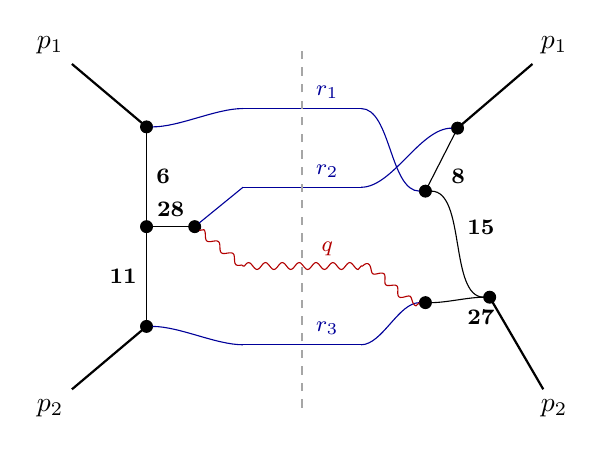
\begin{tikzpicture}
\begin{feynman}
\vertex (Lp1) at (-3.200,2.300) {$p_1$};
\vertex (Lp2) at (-3.200,-2.300) {$p_2$};
\vertex (Lcr1) at (-0.750,1.500);
\vertex (Lcr2) at (-0.750,0.500);
\vertex (Lcr3) at (-0.750,-1.500);
\vertex (Lcq) at (-0.750,-0.500);
\vertex[dot] (L6) at (-1.975,1.267) {};
\vertex[dot] (L28) at (-1.975,0.000) {};
\vertex[dot] (L11) at (-1.975,-1.267) {};
\vertex[dot] (Lroot) at (-1.363,0.000) {};
\vertex (Rp1) at (3.200,2.300) {$p_1$};
\vertex (Rp2) at (3.200,-2.300) {$p_2$};
\vertex (Rcr1) at (0.750,1.500);
\vertex (Rcr2) at (0.750,0.500);
\vertex (Rcr3) at (0.750,-1.500);
\vertex (Rcq) at (0.750,-0.500);
\vertex[dot] (R8) at (1.975,1.251) {};
\vertex[dot] (R15) at (1.567,0.451) {};
\vertex[dot] (R27) at (2.383,-0.896) {};
\vertex[dot] (Rroot) at (1.567,-0.965) {};
\diagram* {
(L6) -- [plain, edge label={\footnotesize\bfseries 6}] (L28),
(L11) -- [plain, edge label={\footnotesize\bfseries 11}] (L28),
(L28) -- [plain, edge label={\footnotesize\bfseries 28}] (Lroot),
(Lp1) -- [plain, thick] (L6),
(Lp2) -- [plain, thick] (L11),
(Lcr1) -- [plain, blue!60!black, out=180, in=0, looseness=0.75] (L6),
(Lcr2) -- [plain, blue!60!black] (Lroot),
(Lcr3) -- [plain, blue!60!black, out=180, in=0, looseness=0.75] (L11),
(Lcq) -- [boson, red!70!black] (Lroot),
(R8) -- [plain, edge label={\footnotesize\bfseries 8}] (R15),
(R15) -- [plain, out=0, in=180, looseness=0.75, edge label={\footnotesize\bfseries 15}] (R27),
(R27) -- [plain, out=180, in=0, looseness=0.75, edge label={\footnotesize\bfseries 27}] (Rroot),
(Rp1) -- [plain, thick] (R8),
(Rp2) -- [plain, thick] (R27),
(Rcr1) -- [plain, blue!60!black, out=0, in=180, looseness=0.75] (R15),
(Rcr2) -- [plain, blue!60!black, out=0, in=180, looseness=0.75] (R8),
(Rcr3) -- [plain, blue!60!black, out=0, in=180, looseness=0.75] (Rroot),
(Rcq) -- [boson, red!70!black, out=0, in=180, looseness=0.75] (Rroot),
(Lcr1) -- [plain, blue!60!black] (Rcr1),
(Lcr2) -- [plain, blue!60!black] (Rcr2),
(Lcr3) -- [plain, blue!60!black] (Rcr3),
(Lcq) -- [boson, red!70!black] (Rcq),
};
\end{feynman}
\draw[dashed, gray!70] (0,-2.30) -- (0,2.30);
\node[font=\footnotesize, blue!60!black, above] at (0.32,1.50) {$r_1$};
\node[font=\footnotesize, blue!60!black, above] at (0.32,0.50) {$r_2$};
\node[font=\footnotesize, blue!60!black, above] at (0.32,-1.50) {$r_3$};
\node[font=\footnotesize, red!70!black, above] at (0.32,-0.50) {$q$};
\end{tikzpicture}}\\[2mm]\textbf{FAM[241]} (topo241)\\[2pt]{\footnotesize\begin{tabular}{@{}r@{\ \ }l@{\ \ }l@{}}\textbf{6} & $(p_1+r_1)^2$ & amplitude\\
\textbf{11} & $(p_2+r_3)^2$ & amplitude\\
\textbf{28} & $(p_1+p_2+r_1+r_3)^2$ & amplitude\\
\textbf{8} & $(p_1+r_2)^2$ & conjugate\\
\textbf{15} & $(p_1+r_1+r_2)^2$ & conjugate\\
\textbf{27} & $(p_1+p_2+r_1+r_2)^2$ & conjugate\\\end{tabular}}\\[2pt]{\scriptsize irreducible numerators: 17 = $(p_1+r_1+r_3)^2$}\end{minipage}\hfill%
\begin{minipage}[t]{0.48\textwidth}\centering\resizebox{0.9\linewidth}{!}{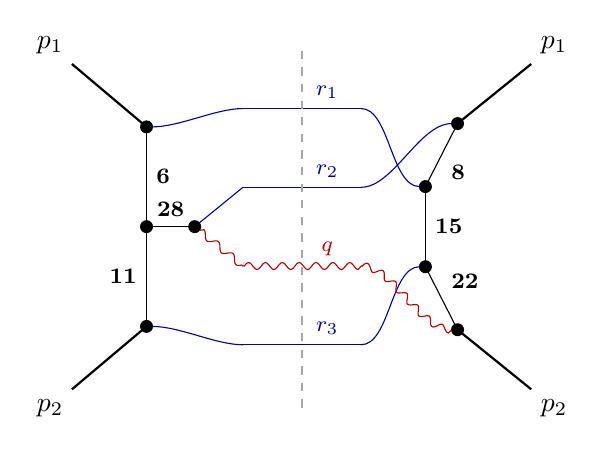
\begin{tikzpicture}
\begin{feynman}
\vertex (Lp1) at (-3.200,2.300) {$p_1$};
\vertex (Lp2) at (-3.200,-2.300) {$p_2$};
\vertex (Lcr1) at (-0.750,1.500);
\vertex (Lcr2) at (-0.750,0.500);
\vertex (Lcr3) at (-0.750,-1.500);
\vertex (Lcq) at (-0.750,-0.500);
\vertex[dot] (L6) at (-1.975,1.267) {};
\vertex[dot] (L28) at (-1.975,0.000) {};
\vertex[dot] (L11) at (-1.975,-1.267) {};
\vertex[dot] (Lroot) at (-1.363,0.000) {};
\vertex (Rp1) at (3.200,2.300) {$p_1$};
\vertex (Rp2) at (3.200,-2.300) {$p_2$};
\vertex (Rcr1) at (0.750,1.500);
\vertex (Rcr2) at (0.750,0.500);
\vertex (Rcr3) at (0.750,-1.500);
\vertex (Rcq) at (0.750,-0.500);
\vertex[dot] (R8) at (1.975,1.309) {};
\vertex[dot] (R15) at (1.567,0.509) {};
\vertex[dot] (R22) at (1.567,-0.509) {};
\vertex[dot] (Rroot) at (1.975,-1.309) {};
\diagram* {
(L6) -- [plain, edge label={\footnotesize\bfseries 6}] (L28),
(L11) -- [plain, edge label={\footnotesize\bfseries 11}] (L28),
(L28) -- [plain, edge label={\footnotesize\bfseries 28}] (Lroot),
(Lp1) -- [plain, thick] (L6),
(Lp2) -- [plain, thick] (L11),
(Lcr1) -- [plain, blue!60!black, out=180, in=0, looseness=0.75] (L6),
(Lcr2) -- [plain, blue!60!black] (Lroot),
(Lcr3) -- [plain, blue!60!black, out=180, in=0, looseness=0.75] (L11),
(Lcq) -- [boson, red!70!black] (Lroot),
(R8) -- [plain, edge label={\footnotesize\bfseries 8}] (R15),
(R15) -- [plain, edge label={\footnotesize\bfseries 15}] (R22),
(R22) -- [plain, edge label={\footnotesize\bfseries 22}] (Rroot),
(Rp1) -- [plain, thick] (R8),
(Rp2) -- [plain, thick] (Rroot),
(Rcr1) -- [plain, blue!60!black, out=0, in=180, looseness=0.75] (R15),
(Rcr2) -- [plain, blue!60!black, out=0, in=180, looseness=0.75] (R8),
(Rcr3) -- [plain, blue!60!black, out=0, in=180, looseness=0.75] (R22),
(Rcq) -- [boson, red!70!black, out=0, in=180, looseness=0.75] (Rroot),
(Lcr1) -- [plain, blue!60!black] (Rcr1),
(Lcr2) -- [plain, blue!60!black] (Rcr2),
(Lcr3) -- [plain, blue!60!black] (Rcr3),
(Lcq) -- [boson, red!70!black] (Rcq),
};
\end{feynman}
\draw[dashed, gray!70] (0,-2.30) -- (0,2.30);
\node[font=\footnotesize, blue!60!black, above] at (0.32,1.50) {$r_1$};
\node[font=\footnotesize, blue!60!black, above] at (0.32,0.50) {$r_2$};
\node[font=\footnotesize, blue!60!black, above] at (0.32,-1.50) {$r_3$};
\node[font=\footnotesize, red!70!black, above] at (0.32,-0.50) {$q$};
\end{tikzpicture}}\\[2mm]\textbf{FAM[247]} (topo247)\\[2pt]{\footnotesize\begin{tabular}{@{}r@{\ \ }l@{\ \ }l@{}}\textbf{6} & $(p_1+r_1)^2$ & amplitude\\
\textbf{11} & $(p_2+r_3)^2$ & amplitude\\
\textbf{28} & $(p_1+p_2+r_1+r_3)^2$ & amplitude\\
\textbf{8} & $(p_1+r_2)^2$ & conjugate\\
\textbf{15} & $(p_1+r_1+r_2)^2$ & conjugate\\
\textbf{22} & $(p_1+r_1+r_2+r_3)^2$ & conjugate\\\end{tabular}}\\[2pt]{\scriptsize irreducible numerators: 24 = $(p_1+p_2+r_1)^2$}\end{minipage}

\bigskip

\begin{minipage}[t]{0.48\textwidth}\centering\resizebox{0.9\linewidth}{!}{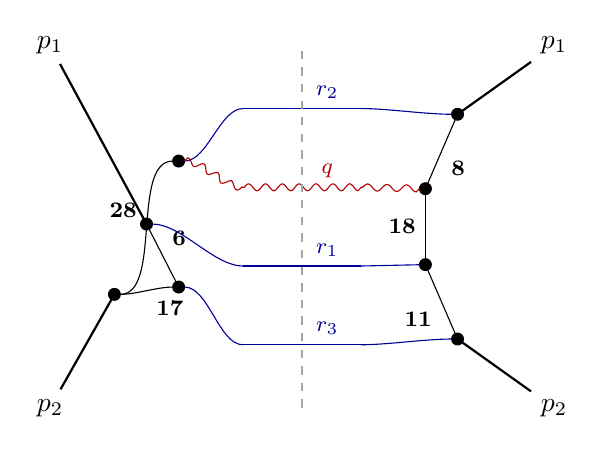
\begin{tikzpicture}
\begin{feynman}
\vertex (Lp1) at (-3.200,2.300) {$p_1$};
\vertex (Lp2) at (-3.200,-2.300) {$p_2$};
\vertex (Lcr1) at (-0.750,-0.500);
\vertex (Lcr2) at (-0.750,1.500);
\vertex (Lcr3) at (-0.750,-1.500);
\vertex (Lcq) at (-0.750,0.500);
\vertex[dot] (L6) at (-1.975,0.033) {};
\vertex[dot] (L17) at (-1.567,-0.767) {};
\vertex[dot] (L28) at (-2.383,-0.860) {};
\vertex[dot] (Lroot) at (-1.567,0.833) {};
\vertex (Rp1) at (3.200,2.300) {$p_1$};
\vertex (Rp2) at (3.200,-2.300) {$p_2$};
\vertex (Rcr1) at (0.750,-0.500);
\vertex (Rcr2) at (0.750,1.500);
\vertex (Rcr3) at (0.750,-1.500);
\vertex (Rcq) at (0.750,0.500);
\vertex[dot] (R8) at (1.975,1.427) {};
\vertex[dot] (Rroot) at (1.567,0.482) {};
\vertex[dot] (R11) at (1.975,-1.427) {};
\vertex[dot] (R18) at (1.567,-0.482) {};
\diagram* {
(L6) -- [plain, edge label={\footnotesize\bfseries 6}] (L17),
(L17) -- [plain, out=180, in=0, looseness=0.75, edge label={\footnotesize\bfseries 17}] (L28),
(L28) -- [plain, out=0, in=180, looseness=0.75, edge label={\footnotesize\bfseries 28}] (Lroot),
(Lp1) -- [plain, thick] (L6),
(Lp2) -- [plain, thick] (L28),
(Lcr1) -- [plain, blue!60!black, out=180, in=0, looseness=0.75] (L6),
(Lcr2) -- [plain, blue!60!black, out=180, in=0, looseness=0.75] (Lroot),
(Lcr3) -- [plain, blue!60!black, out=180, in=0, looseness=0.75] (L17),
(Lcq) -- [boson, red!70!black, out=180, in=0, looseness=0.75] (Lroot),
(R8) -- [plain, edge label={\footnotesize\bfseries 8}] (Rroot),
(R11) -- [plain, edge label={\footnotesize\bfseries 11}] (R18),
(R18) -- [plain, edge label={\footnotesize\bfseries 18}] (Rroot),
(Rp1) -- [plain, thick] (R8),
(Rp2) -- [plain, thick] (R11),
(Rcr1) -- [plain, blue!60!black] (R18),
(Rcr2) -- [plain, blue!60!black, out=0, in=180, looseness=0.75] (R8),
(Rcr3) -- [plain, blue!60!black, out=0, in=180, looseness=0.75] (R11),
(Rcq) -- [boson, red!70!black] (Rroot),
(Lcr1) -- [plain, blue!60!black] (Rcr1),
(Lcr2) -- [plain, blue!60!black] (Rcr2),
(Lcr3) -- [plain, blue!60!black] (Rcr3),
(Lcq) -- [boson, red!70!black] (Rcq),
};
\end{feynman}
\draw[dashed, gray!70] (0,-2.30) -- (0,2.30);
\node[font=\footnotesize, blue!60!black, above] at (0.32,-0.50) {$r_1$};
\node[font=\footnotesize, blue!60!black, above] at (0.32,1.50) {$r_2$};
\node[font=\footnotesize, blue!60!black, above] at (0.32,-1.50) {$r_3$};
\node[font=\footnotesize, red!70!black, above] at (0.32,0.50) {$q$};
\end{tikzpicture}}\\[2mm]\textbf{FAM[253]} (topo253)\\[2pt]{\footnotesize\begin{tabular}{@{}r@{\ \ }l@{\ \ }l@{}}\textbf{6} & $(p_1+r_1)^2$ & amplitude\\
\textbf{17} & $(p_1+r_1+r_3)^2$ & amplitude\\
\textbf{28} & $(p_1+p_2+r_1+r_3)^2$ & amplitude\\
\textbf{8} & $(p_1+r_2)^2$ & conjugate\\
\textbf{11} & $(p_2+r_3)^2$ & conjugate\\
\textbf{18} & $(p_2+r_1+r_3)^2$ & conjugate\\\end{tabular}}\\[2pt]{\scriptsize irreducible numerators: 29 = $(p_1+p_2+r_2+r_3)^2$}\end{minipage}\hfill%
\begin{minipage}[t]{0.48\textwidth}\centering\resizebox{0.9\linewidth}{!}{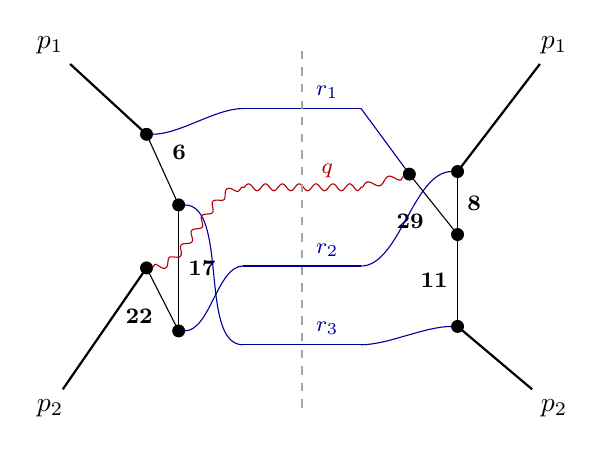
\begin{tikzpicture}
\begin{feynman}
\vertex (Lp1) at (-3.200,2.300) {$p_1$};
\vertex (Lp2) at (-3.200,-2.300) {$p_2$};
\vertex (Lcr1) at (-0.750,1.500);
\vertex (Lcr2) at (-0.750,-0.500);
\vertex (Lcr3) at (-0.750,-1.500);
\vertex (Lcq) at (-0.750,0.500);
\vertex[dot] (L6) at (-1.975,1.173) {};
\vertex[dot] (L17) at (-1.567,0.276) {};
\vertex[dot] (L22) at (-1.567,-1.324) {};
\vertex[dot] (Lroot) at (-1.975,-0.524) {};
\vertex (Rp1) at (3.200,2.300) {$p_1$};
\vertex (Rp2) at (3.200,-2.300) {$p_2$};
\vertex (Rcr1) at (0.750,1.500);
\vertex (Rcr2) at (0.750,-0.500);
\vertex (Rcr3) at (0.750,-1.500);
\vertex (Rcq) at (0.750,0.500);
\vertex[dot] (R8) at (1.975,0.700) {};
\vertex[dot] (R29) at (1.975,-0.100) {};
\vertex[dot] (R11) at (1.975,-1.267) {};
\vertex[dot] (Rroot) at (1.363,0.667) {};
\diagram* {
(L6) -- [plain, edge label={\footnotesize\bfseries 6}] (L17),
(L17) -- [plain, edge label={\footnotesize\bfseries 17}] (L22),
(L22) -- [plain, edge label={\footnotesize\bfseries 22}] (Lroot),
(Lp1) -- [plain, thick] (L6),
(Lp2) -- [plain, thick] (Lroot),
(Lcr1) -- [plain, blue!60!black, out=180, in=0, looseness=0.75] (L6),
(Lcr2) -- [plain, blue!60!black, out=180, in=0, looseness=0.75] (L22),
(Lcr3) -- [plain, blue!60!black, out=180, in=0, looseness=0.75] (L17),
(Lcq) -- [boson, red!70!black, out=180, in=0, looseness=0.75] (Lroot),
(R8) -- [plain, edge label={\footnotesize\bfseries 8}] (R29),
(R11) -- [plain, edge label={\footnotesize\bfseries 11}] (R29),
(R29) -- [plain, edge label={\footnotesize\bfseries 29}] (Rroot),
(Rp1) -- [plain, thick] (R8),
(Rp2) -- [plain, thick] (R11),
(Rcr1) -- [plain, blue!60!black] (Rroot),
(Rcr2) -- [plain, blue!60!black, out=0, in=180, looseness=0.75] (R8),
(Rcr3) -- [plain, blue!60!black, out=0, in=180, looseness=0.75] (R11),
(Rcq) -- [boson, red!70!black] (Rroot),
(Lcr1) -- [plain, blue!60!black] (Rcr1),
(Lcr2) -- [plain, blue!60!black] (Rcr2),
(Lcr3) -- [plain, blue!60!black] (Rcr3),
(Lcq) -- [boson, red!70!black] (Rcq),
};
\end{feynman}
\draw[dashed, gray!70] (0,-2.30) -- (0,2.30);
\node[font=\footnotesize, blue!60!black, above] at (0.32,1.50) {$r_1$};
\node[font=\footnotesize, blue!60!black, above] at (0.32,-0.50) {$r_2$};
\node[font=\footnotesize, blue!60!black, above] at (0.32,-1.50) {$r_3$};
\node[font=\footnotesize, red!70!black, above] at (0.32,0.50) {$q$};
\end{tikzpicture}}\\[2mm]\textbf{FAM[259]} (topo259)\\[2pt]{\footnotesize\begin{tabular}{@{}r@{\ \ }l@{\ \ }l@{}}\textbf{6} & $(p_1+r_1)^2$ & amplitude\\
\textbf{17} & $(p_1+r_1+r_3)^2$ & amplitude\\
\textbf{22} & $(p_1+r_1+r_2+r_3)^2$ & amplitude\\
\textbf{8} & $(p_1+r_2)^2$ & conjugate\\
\textbf{11} & $(p_2+r_3)^2$ & conjugate\\
\textbf{29} & $(p_1+p_2+r_2+r_3)^2$ & conjugate\\\end{tabular}}\\[2pt]{\scriptsize irreducible numerators: 25 = $(p_1+p_2+r_2)^2$}\end{minipage}

\bigskip

\begin{minipage}[t]{0.48\textwidth}\centering\resizebox{0.9\linewidth}{!}{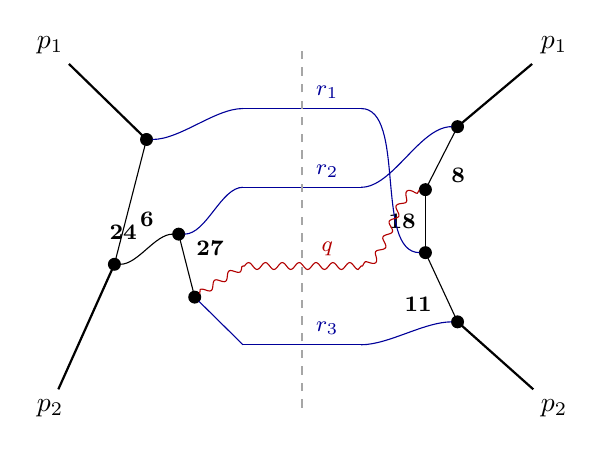
\begin{tikzpicture}
\begin{feynman}
\vertex (Lp1) at (-3.200,2.300) {$p_1$};
\vertex (Lp2) at (-3.200,-2.300) {$p_2$};
\vertex (Lcr1) at (-0.750,1.500);
\vertex (Lcr2) at (-0.750,0.500);
\vertex (Lcr3) at (-0.750,-1.500);
\vertex (Lcq) at (-0.750,-0.500);
\vertex[dot] (L6) at (-1.975,1.107) {};
\vertex[dot] (L24) at (-2.383,-0.478) {};
\vertex[dot] (L27) at (-1.567,-0.095) {};
\vertex[dot] (Lroot) at (-1.363,-0.895) {};
\vertex (Rp1) at (3.200,2.300) {$p_1$};
\vertex (Rp2) at (3.200,-2.300) {$p_2$};
\vertex (Rcr1) at (0.750,1.500);
\vertex (Rcr2) at (0.750,0.500);
\vertex (Rcr3) at (0.750,-1.500);
\vertex (Rcq) at (0.750,-0.500);
\vertex[dot] (R8) at (1.975,1.270) {};
\vertex[dot] (Rroot) at (1.567,0.470) {};
\vertex[dot] (R11) at (1.975,-1.209) {};
\vertex[dot] (R18) at (1.567,-0.330) {};
\diagram* {
(L6) -- [plain, edge label={\footnotesize\bfseries 6}] (L24),
(L24) -- [plain, out=0, in=180, looseness=0.75, edge label={\footnotesize\bfseries 24}] (L27),
(L27) -- [plain, edge label={\footnotesize\bfseries 27}] (Lroot),
(Lp1) -- [plain, thick] (L6),
(Lp2) -- [plain, thick] (L24),
(Lcr1) -- [plain, blue!60!black, out=180, in=0, looseness=0.75] (L6),
(Lcr2) -- [plain, blue!60!black, out=180, in=0, looseness=0.75] (L27),
(Lcr3) -- [plain, blue!60!black] (Lroot),
(Lcq) -- [boson, red!70!black] (Lroot),
(R8) -- [plain, edge label={\footnotesize\bfseries 8}] (Rroot),
(R11) -- [plain, edge label={\footnotesize\bfseries 11}] (R18),
(R18) -- [plain, edge label={\footnotesize\bfseries 18}] (Rroot),
(Rp1) -- [plain, thick] (R8),
(Rp2) -- [plain, thick] (R11),
(Rcr1) -- [plain, blue!60!black, out=0, in=180, looseness=0.75] (R18),
(Rcr2) -- [plain, blue!60!black, out=0, in=180, looseness=0.75] (R8),
(Rcr3) -- [plain, blue!60!black, out=0, in=180, looseness=0.75] (R11),
(Rcq) -- [boson, red!70!black, out=0, in=180, looseness=0.75] (Rroot),
(Lcr1) -- [plain, blue!60!black] (Rcr1),
(Lcr2) -- [plain, blue!60!black] (Rcr2),
(Lcr3) -- [plain, blue!60!black] (Rcr3),
(Lcq) -- [boson, red!70!black] (Rcq),
};
\end{feynman}
\draw[dashed, gray!70] (0,-2.30) -- (0,2.30);
\node[font=\footnotesize, blue!60!black, above] at (0.32,1.50) {$r_1$};
\node[font=\footnotesize, blue!60!black, above] at (0.32,0.50) {$r_2$};
\node[font=\footnotesize, blue!60!black, above] at (0.32,-1.50) {$r_3$};
\node[font=\footnotesize, red!70!black, above] at (0.32,-0.50) {$q$};
\end{tikzpicture}}\\[2mm]\textbf{FAM[265]} (topo265)\\[2pt]{\footnotesize\begin{tabular}{@{}r@{\ \ }l@{\ \ }l@{}}\textbf{6} & $(p_1+r_1)^2$ & amplitude\\
\textbf{24} & $(p_1+p_2+r_1)^2$ & amplitude\\
\textbf{27} & $(p_1+p_2+r_1+r_2)^2$ & amplitude\\
\textbf{8} & $(p_1+r_2)^2$ & conjugate\\
\textbf{11} & $(p_2+r_3)^2$ & conjugate\\
\textbf{18} & $(p_2+r_1+r_3)^2$ & conjugate\\\end{tabular}}\\[2pt]{\scriptsize irreducible numerators: 23 = $(p_2+r_1+r_2+r_3)^2$}\end{minipage}\hfill%
\begin{minipage}[t]{0.48\textwidth}\centering\resizebox{0.9\linewidth}{!}{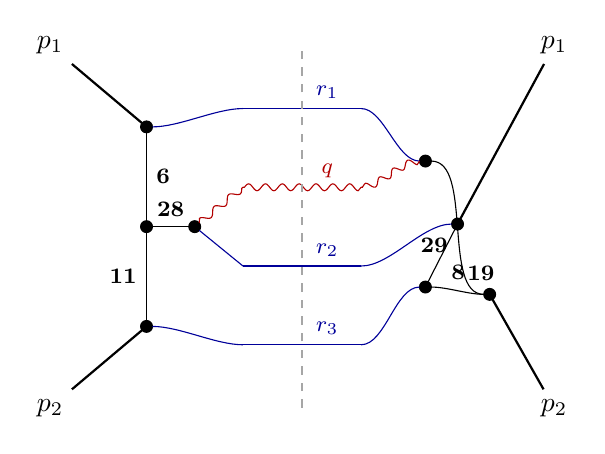
\begin{tikzpicture}
\begin{feynman}
\vertex (Lp1) at (-3.200,2.300) {$p_1$};
\vertex (Lp2) at (-3.200,-2.300) {$p_2$};
\vertex (Lcr1) at (-0.750,1.500);
\vertex (Lcr2) at (-0.750,-0.500);
\vertex (Lcr3) at (-0.750,-1.500);
\vertex (Lcq) at (-0.750,0.500);
\vertex[dot] (L6) at (-1.975,1.267) {};
\vertex[dot] (L28) at (-1.975,0.000) {};
\vertex[dot] (L11) at (-1.975,-1.267) {};
\vertex[dot] (Lroot) at (-1.363,0.000) {};
\vertex (Rp1) at (3.200,2.300) {$p_1$};
\vertex (Rp2) at (3.200,-2.300) {$p_2$};
\vertex (Rcr1) at (0.750,1.500);
\vertex (Rcr2) at (0.750,-0.500);
\vertex (Rcr3) at (0.750,-1.500);
\vertex (Rcq) at (0.750,0.500);
\vertex[dot] (R8) at (1.975,0.033) {};
\vertex[dot] (R19) at (1.567,-0.767) {};
\vertex[dot] (R29) at (2.383,-0.860) {};
\vertex[dot] (Rroot) at (1.567,0.833) {};
\diagram* {
(L6) -- [plain, edge label={\footnotesize\bfseries 6}] (L28),
(L11) -- [plain, edge label={\footnotesize\bfseries 11}] (L28),
(L28) -- [plain, edge label={\footnotesize\bfseries 28}] (Lroot),
(Lp1) -- [plain, thick] (L6),
(Lp2) -- [plain, thick] (L11),
(Lcr1) -- [plain, blue!60!black, out=180, in=0, looseness=0.75] (L6),
(Lcr2) -- [plain, blue!60!black] (Lroot),
(Lcr3) -- [plain, blue!60!black, out=180, in=0, looseness=0.75] (L11),
(Lcq) -- [boson, red!70!black] (Lroot),
(R8) -- [plain, edge label={\footnotesize\bfseries 8}] (R19),
(R19) -- [plain, out=0, in=180, looseness=0.75, edge label={\footnotesize\bfseries 19}] (R29),
(R29) -- [plain, out=180, in=0, looseness=0.75, edge label={\footnotesize\bfseries 29}] (Rroot),
(Rp1) -- [plain, thick] (R8),
(Rp2) -- [plain, thick] (R29),
(Rcr1) -- [plain, blue!60!black, out=0, in=180, looseness=0.75] (Rroot),
(Rcr2) -- [plain, blue!60!black, out=0, in=180, looseness=0.75] (R8),
(Rcr3) -- [plain, blue!60!black, out=0, in=180, looseness=0.75] (R19),
(Rcq) -- [boson, red!70!black, out=0, in=180, looseness=0.75] (Rroot),
(Lcr1) -- [plain, blue!60!black] (Rcr1),
(Lcr2) -- [plain, blue!60!black] (Rcr2),
(Lcr3) -- [plain, blue!60!black] (Rcr3),
(Lcq) -- [boson, red!70!black] (Rcq),
};
\end{feynman}
\draw[dashed, gray!70] (0,-2.30) -- (0,2.30);
\node[font=\footnotesize, blue!60!black, above] at (0.32,1.50) {$r_1$};
\node[font=\footnotesize, blue!60!black, above] at (0.32,-0.50) {$r_2$};
\node[font=\footnotesize, blue!60!black, above] at (0.32,-1.50) {$r_3$};
\node[font=\footnotesize, red!70!black, above] at (0.32,0.50) {$q$};
\end{tikzpicture}}\\[2mm]\textbf{FAM[271]} (topo271)\\[2pt]{\footnotesize\begin{tabular}{@{}r@{\ \ }l@{\ \ }l@{}}\textbf{6} & $(p_1+r_1)^2$ & amplitude\\
\textbf{11} & $(p_2+r_3)^2$ & amplitude\\
\textbf{28} & $(p_1+p_2+r_1+r_3)^2$ & amplitude\\
\textbf{8} & $(p_1+r_2)^2$ & conjugate\\
\textbf{19} & $(p_1+r_2+r_3)^2$ & conjugate\\
\textbf{29} & $(p_1+p_2+r_2+r_3)^2$ & conjugate\\\end{tabular}}\\[2pt]{\scriptsize irreducible numerators: 24 = $(p_1+p_2+r_1)^2$}\end{minipage}

\bigskip

\begin{minipage}[t]{0.48\textwidth}\centering\resizebox{0.9\linewidth}{!}{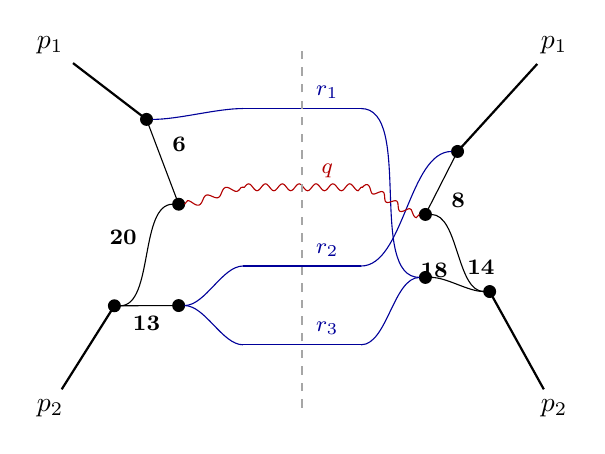
\begin{tikzpicture}
\begin{feynman}
\vertex (Lp1) at (-3.200,2.300) {$p_1$};
\vertex (Lp2) at (-3.200,-2.300) {$p_2$};
\vertex (Lcr1) at (-0.750,1.500);
\vertex (Lcr2) at (-0.750,-0.500);
\vertex (Lcr3) at (-0.750,-1.500);
\vertex (Lcq) at (-0.750,0.500);
\vertex[dot] (L6) at (-1.975,1.362) {};
\vertex[dot] (Lroot) at (-1.567,0.285) {};
\vertex[dot] (L13) at (-1.567,-1.002) {};
\vertex[dot] (L20) at (-2.383,-1.005) {};
\vertex (Rp1) at (3.200,2.300) {$p_1$};
\vertex (Rp2) at (3.200,-2.300) {$p_2$};
\vertex (Rcr1) at (0.750,1.500);
\vertex (Rcr2) at (0.750,-0.500);
\vertex (Rcr3) at (0.750,-1.500);
\vertex (Rcq) at (0.750,0.500);
\vertex[dot] (R8) at (1.975,0.955) {};
\vertex[dot] (Rroot) at (1.567,0.155) {};
\vertex[dot] (R14) at (1.567,-0.645) {};
\vertex[dot] (R18) at (2.383,-0.824) {};
\diagram* {
(L6) -- [plain, edge label={\footnotesize\bfseries 6}] (Lroot),
(L13) -- [plain, edge label={\footnotesize\bfseries 13}] (L20),
(L20) -- [plain, out=0, in=180, looseness=0.75, edge label={\footnotesize\bfseries 20}] (Lroot),
(Lp1) -- [plain, thick] (L6),
(Lp2) -- [plain, thick] (L20),
(Lcr1) -- [plain, blue!60!black, out=180, in=0, looseness=0.75] (L6),
(Lcr2) -- [plain, blue!60!black, out=180, in=0, looseness=0.75] (L13),
(Lcr3) -- [plain, blue!60!black, out=180, in=0, looseness=0.75] (L13),
(Lcq) -- [boson, red!70!black, out=180, in=0, looseness=0.75] (Lroot),
(R8) -- [plain, edge label={\footnotesize\bfseries 8}] (Rroot),
(R14) -- [plain, out=0, in=180, looseness=0.75, edge label={\footnotesize\bfseries 14}] (R18),
(R18) -- [plain, out=180, in=0, looseness=0.75, edge label={\footnotesize\bfseries 18}] (Rroot),
(Rp1) -- [plain, thick] (R8),
(Rp2) -- [plain, thick] (R18),
(Rcr1) -- [plain, blue!60!black, out=0, in=180, looseness=0.75] (R14),
(Rcr2) -- [plain, blue!60!black, out=0, in=180, looseness=0.75] (R8),
(Rcr3) -- [plain, blue!60!black, out=0, in=180, looseness=0.75] (R14),
(Rcq) -- [boson, red!70!black, out=0, in=180, looseness=0.75] (Rroot),
(Lcr1) -- [plain, blue!60!black] (Rcr1),
(Lcr2) -- [plain, blue!60!black] (Rcr2),
(Lcr3) -- [plain, blue!60!black] (Rcr3),
(Lcq) -- [boson, red!70!black] (Rcq),
};
\end{feynman}
\draw[dashed, gray!70] (0,-2.30) -- (0,2.30);
\node[font=\footnotesize, blue!60!black, above] at (0.32,1.50) {$r_1$};
\node[font=\footnotesize, blue!60!black, above] at (0.32,-0.50) {$r_2$};
\node[font=\footnotesize, blue!60!black, above] at (0.32,-1.50) {$r_3$};
\node[font=\footnotesize, red!70!black, above] at (0.32,0.50) {$q$};
\end{tikzpicture}}\\[2mm]\textbf{FAM[277]} (topo277)\\[2pt]{\footnotesize\begin{tabular}{@{}r@{\ \ }l@{\ \ }l@{}}\textbf{6} & $(p_1+r_1)^2$ & amplitude\\
\textbf{13} & $(r_2+r_3)^2$ & amplitude\\
\textbf{20} & $(p_2+r_2+r_3)^2$ & amplitude\\
\textbf{8} & $(p_1+r_2)^2$ & conjugate\\
\textbf{14} & $(r_1+r_3)^2$ & conjugate\\
\textbf{18} & $(p_2+r_1+r_3)^2$ & conjugate\\\end{tabular}}\\[2pt]{\scriptsize irreducible numerators: 21 = $(r_1+r_2+r_3)^2$}\end{minipage}\hfill%
\begin{minipage}[t]{0.48\textwidth}\centering\resizebox{0.9\linewidth}{!}{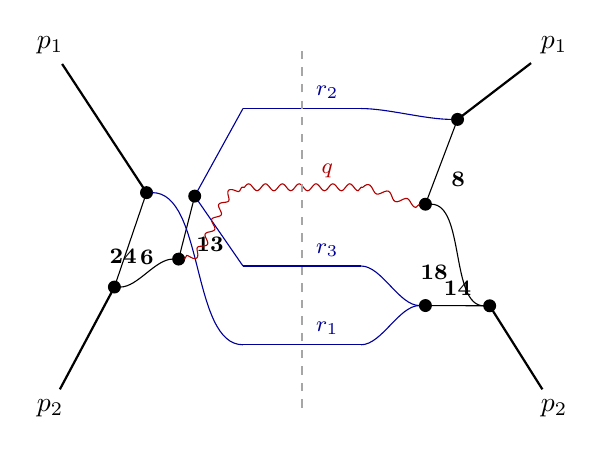
\begin{tikzpicture}
\begin{feynman}
\vertex (Lp1) at (-3.200,2.300) {$p_1$};
\vertex (Lp2) at (-3.200,-2.300) {$p_2$};
\vertex (Lcr1) at (-0.750,-1.500);
\vertex (Lcr2) at (-0.750,1.500);
\vertex (Lcr3) at (-0.750,-0.500);
\vertex (Lcq) at (-0.750,0.500);
\vertex[dot] (L6) at (-1.975,0.432) {};
\vertex[dot] (L24) at (-2.383,-0.767) {};
\vertex[dot] (L13) at (-1.363,0.388) {};
\vertex[dot] (Lroot) at (-1.567,-0.412) {};
\vertex (Rp1) at (3.200,2.300) {$p_1$};
\vertex (Rp2) at (3.200,-2.300) {$p_2$};
\vertex (Rcr1) at (0.750,-1.500);
\vertex (Rcr2) at (0.750,1.500);
\vertex (Rcr3) at (0.750,-0.500);
\vertex (Rcq) at (0.750,0.500);
\vertex[dot] (R8) at (1.975,1.362) {};
\vertex[dot] (Rroot) at (1.567,0.285) {};
\vertex[dot] (R14) at (1.567,-1.002) {};
\vertex[dot] (R18) at (2.383,-1.005) {};
\diagram* {
(L6) -- [plain, edge label={\footnotesize\bfseries 6}] (L24),
(L13) -- [plain, edge label={\footnotesize\bfseries 13}] (Lroot),
(L24) -- [plain, out=0, in=180, looseness=0.75, edge label={\footnotesize\bfseries 24}] (Lroot),
(Lp1) -- [plain, thick] (L6),
(Lp2) -- [plain, thick] (L24),
(Lcr1) -- [plain, blue!60!black, out=180, in=0, looseness=0.75] (L6),
(Lcr2) -- [plain, blue!60!black] (L13),
(Lcr3) -- [plain, blue!60!black] (L13),
(Lcq) -- [boson, red!70!black, out=180, in=0, looseness=0.75] (Lroot),
(R8) -- [plain, edge label={\footnotesize\bfseries 8}] (Rroot),
(R14) -- [plain, edge label={\footnotesize\bfseries 14}] (R18),
(R18) -- [plain, out=180, in=0, looseness=0.75, edge label={\footnotesize\bfseries 18}] (Rroot),
(Rp1) -- [plain, thick] (R8),
(Rp2) -- [plain, thick] (R18),
(Rcr1) -- [plain, blue!60!black, out=0, in=180, looseness=0.75] (R14),
(Rcr2) -- [plain, blue!60!black, out=0, in=180, looseness=0.75] (R8),
(Rcr3) -- [plain, blue!60!black, out=0, in=180, looseness=0.75] (R14),
(Rcq) -- [boson, red!70!black, out=0, in=180, looseness=0.75] (Rroot),
(Lcr1) -- [plain, blue!60!black] (Rcr1),
(Lcr2) -- [plain, blue!60!black] (Rcr2),
(Lcr3) -- [plain, blue!60!black] (Rcr3),
(Lcq) -- [boson, red!70!black] (Rcq),
};
\end{feynman}
\draw[dashed, gray!70] (0,-2.30) -- (0,2.30);
\node[font=\footnotesize, blue!60!black, above] at (0.32,-1.50) {$r_1$};
\node[font=\footnotesize, blue!60!black, above] at (0.32,1.50) {$r_2$};
\node[font=\footnotesize, blue!60!black, above] at (0.32,-0.50) {$r_3$};
\node[font=\footnotesize, red!70!black, above] at (0.32,0.50) {$q$};
\end{tikzpicture}}\\[2mm]\textbf{FAM[280]} (topo280)\\[2pt]{\footnotesize\begin{tabular}{@{}r@{\ \ }l@{\ \ }l@{}}\textbf{6} & $(p_1+r_1)^2$ & amplitude\\
\textbf{13} & $(r_2+r_3)^2$ & amplitude\\
\textbf{24} & $(p_1+p_2+r_1)^2$ & amplitude\\
\textbf{8} & $(p_1+r_2)^2$ & conjugate\\
\textbf{14} & $(r_1+r_3)^2$ & conjugate\\
\textbf{18} & $(p_2+r_1+r_3)^2$ & conjugate\\\end{tabular}}\\[2pt]{\scriptsize irreducible numerators: 28 = $(p_1+p_2+r_1+r_3)^2$}\end{minipage}

\bigskip

\begin{minipage}[t]{0.48\textwidth}\centering\resizebox{0.9\linewidth}{!}{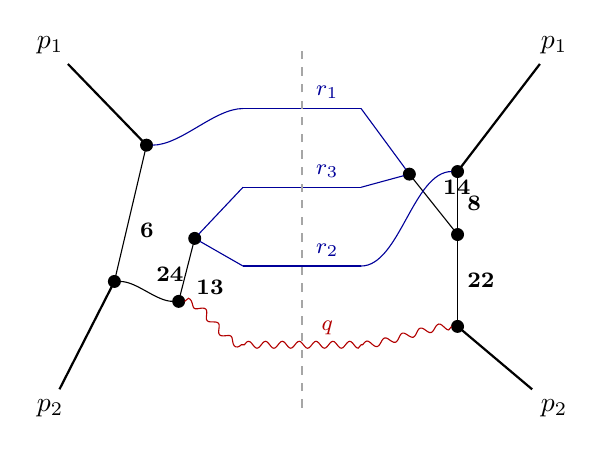
\begin{tikzpicture}
\begin{feynman}
\vertex (Lp1) at (-3.200,2.300) {$p_1$};
\vertex (Lp2) at (-3.200,-2.300) {$p_2$};
\vertex (Lcr1) at (-0.750,1.500);
\vertex (Lcr2) at (-0.750,-0.500);
\vertex (Lcr3) at (-0.750,0.500);
\vertex (Lcq) at (-0.750,-1.500);
\vertex[dot] (L6) at (-1.975,1.035) {};
\vertex[dot] (L24) at (-2.383,-0.696) {};
\vertex[dot] (L13) at (-1.363,-0.149) {};
\vertex[dot] (Lroot) at (-1.567,-0.949) {};
\vertex (Rp1) at (3.200,2.300) {$p_1$};
\vertex (Rp2) at (3.200,-2.300) {$p_2$};
\vertex (Rcr1) at (0.750,1.500);
\vertex (Rcr2) at (0.750,-0.500);
\vertex (Rcr3) at (0.750,0.500);
\vertex (Rcq) at (0.750,-1.500);
\vertex[dot] (R8) at (1.975,0.700) {};
\vertex[dot] (R22) at (1.975,-0.100) {};
\vertex[dot] (R14) at (1.363,0.667) {};
\vertex[dot] (Rroot) at (1.975,-1.267) {};
\diagram* {
(L6) -- [plain, edge label={\footnotesize\bfseries 6}] (L24),
(L13) -- [plain, edge label={\footnotesize\bfseries 13}] (Lroot),
(L24) -- [plain, out=0, in=180, looseness=0.75, edge label={\footnotesize\bfseries 24}] (Lroot),
(Lp1) -- [plain, thick] (L6),
(Lp2) -- [plain, thick] (L24),
(Lcr1) -- [plain, blue!60!black, out=180, in=0, looseness=0.75] (L6),
(Lcr2) -- [plain, blue!60!black] (L13),
(Lcr3) -- [plain, blue!60!black] (L13),
(Lcq) -- [boson, red!70!black, out=180, in=0, looseness=0.75] (Lroot),
(R8) -- [plain, edge label={\footnotesize\bfseries 8}] (R22),
(R14) -- [plain, edge label={\footnotesize\bfseries 14}] (R22),
(R22) -- [plain, edge label={\footnotesize\bfseries 22}] (Rroot),
(Rp1) -- [plain, thick] (R8),
(Rp2) -- [plain, thick] (Rroot),
(Rcr1) -- [plain, blue!60!black] (R14),
(Rcr2) -- [plain, blue!60!black, out=0, in=180, looseness=0.75] (R8),
(Rcr3) -- [plain, blue!60!black] (R14),
(Rcq) -- [boson, red!70!black, out=0, in=180, looseness=0.75] (Rroot),
(Lcr1) -- [plain, blue!60!black] (Rcr1),
(Lcr2) -- [plain, blue!60!black] (Rcr2),
(Lcr3) -- [plain, blue!60!black] (Rcr3),
(Lcq) -- [boson, red!70!black] (Rcq),
};
\end{feynman}
\draw[dashed, gray!70] (0,-2.30) -- (0,2.30);
\node[font=\footnotesize, blue!60!black, above] at (0.32,1.50) {$r_1$};
\node[font=\footnotesize, blue!60!black, above] at (0.32,-0.50) {$r_2$};
\node[font=\footnotesize, blue!60!black, above] at (0.32,0.50) {$r_3$};
\node[font=\footnotesize, red!70!black, above] at (0.32,-1.50) {$q$};
\end{tikzpicture}}\\[2mm]\textbf{FAM[286]} (topo286)\\[2pt]{\footnotesize\begin{tabular}{@{}r@{\ \ }l@{\ \ }l@{}}\textbf{6} & $(p_1+r_1)^2$ & amplitude\\
\textbf{13} & $(r_2+r_3)^2$ & amplitude\\
\textbf{24} & $(p_1+p_2+r_1)^2$ & amplitude\\
\textbf{8} & $(p_1+r_2)^2$ & conjugate\\
\textbf{14} & $(r_1+r_3)^2$ & conjugate\\
\textbf{22} & $(p_1+r_1+r_2+r_3)^2$ & conjugate\\\end{tabular}}\\[2pt]{\scriptsize irreducible numerators: 27 = $(p_1+p_2+r_1+r_2)^2$}\end{minipage}\hfill%
\begin{minipage}[t]{0.48\textwidth}\centering\resizebox{0.9\linewidth}{!}{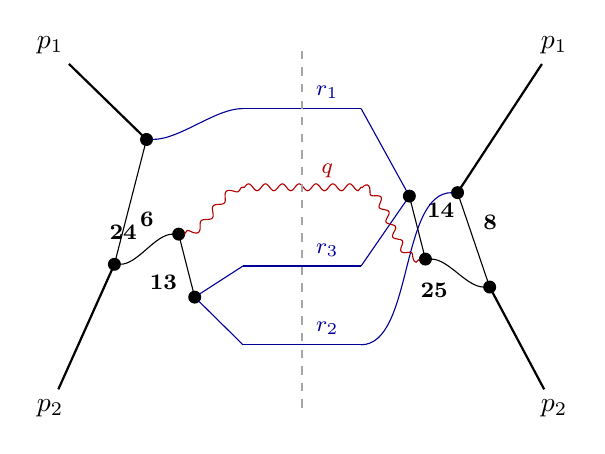
\begin{tikzpicture}
\begin{feynman}
\vertex (Lp1) at (-3.200,2.300) {$p_1$};
\vertex (Lp2) at (-3.200,-2.300) {$p_2$};
\vertex (Lcr1) at (-0.750,1.500);
\vertex (Lcr2) at (-0.750,-1.500);
\vertex (Lcr3) at (-0.750,-0.500);
\vertex (Lcq) at (-0.750,0.500);
\vertex[dot] (L6) at (-1.975,1.107) {};
\vertex[dot] (L24) at (-2.383,-0.478) {};
\vertex[dot] (L13) at (-1.363,-0.895) {};
\vertex[dot] (Lroot) at (-1.567,-0.095) {};
\vertex (Rp1) at (3.200,2.300) {$p_1$};
\vertex (Rp2) at (3.200,-2.300) {$p_2$};
\vertex (Rcr1) at (0.750,1.500);
\vertex (Rcr2) at (0.750,-1.500);
\vertex (Rcr3) at (0.750,-0.500);
\vertex (Rcq) at (0.750,0.500);
\vertex[dot] (R8) at (1.975,0.432) {};
\vertex[dot] (R25) at (2.383,-0.767) {};
\vertex[dot] (R14) at (1.363,0.388) {};
\vertex[dot] (Rroot) at (1.567,-0.412) {};
\diagram* {
(L6) -- [plain, edge label={\footnotesize\bfseries 6}] (L24),
(L13) -- [plain, edge label={\footnotesize\bfseries 13}] (Lroot),
(L24) -- [plain, out=0, in=180, looseness=0.75, edge label={\footnotesize\bfseries 24}] (Lroot),
(Lp1) -- [plain, thick] (L6),
(Lp2) -- [plain, thick] (L24),
(Lcr1) -- [plain, blue!60!black, out=180, in=0, looseness=0.75] (L6),
(Lcr2) -- [plain, blue!60!black] (L13),
(Lcr3) -- [plain, blue!60!black] (L13),
(Lcq) -- [boson, red!70!black, out=180, in=0, looseness=0.75] (Lroot),
(R8) -- [plain, edge label={\footnotesize\bfseries 8}] (R25),
(R14) -- [plain, edge label={\footnotesize\bfseries 14}] (Rroot),
(R25) -- [plain, out=180, in=0, looseness=0.75, edge label={\footnotesize\bfseries 25}] (Rroot),
(Rp1) -- [plain, thick] (R8),
(Rp2) -- [plain, thick] (R25),
(Rcr1) -- [plain, blue!60!black] (R14),
(Rcr2) -- [plain, blue!60!black, out=0, in=180, looseness=0.75] (R8),
(Rcr3) -- [plain, blue!60!black] (R14),
(Rcq) -- [boson, red!70!black, out=0, in=180, looseness=0.75] (Rroot),
(Lcr1) -- [plain, blue!60!black] (Rcr1),
(Lcr2) -- [plain, blue!60!black] (Rcr2),
(Lcr3) -- [plain, blue!60!black] (Rcr3),
(Lcq) -- [boson, red!70!black] (Rcq),
};
\end{feynman}
\draw[dashed, gray!70] (0,-2.30) -- (0,2.30);
\node[font=\footnotesize, blue!60!black, above] at (0.32,1.50) {$r_1$};
\node[font=\footnotesize, blue!60!black, above] at (0.32,-1.50) {$r_2$};
\node[font=\footnotesize, blue!60!black, above] at (0.32,-0.50) {$r_3$};
\node[font=\footnotesize, red!70!black, above] at (0.32,0.50) {$q$};
\end{tikzpicture}}\\[2mm]\textbf{FAM[292]} (topo292)\\[2pt]{\footnotesize\begin{tabular}{@{}r@{\ \ }l@{\ \ }l@{}}\textbf{6} & $(p_1+r_1)^2$ & amplitude\\
\textbf{13} & $(r_2+r_3)^2$ & amplitude\\
\textbf{24} & $(p_1+p_2+r_1)^2$ & amplitude\\
\textbf{8} & $(p_1+r_2)^2$ & conjugate\\
\textbf{14} & $(r_1+r_3)^2$ & conjugate\\
\textbf{25} & $(p_1+p_2+r_2)^2$ & conjugate\\\end{tabular}}\\[2pt]{\scriptsize irreducible numerators: 17 = $(p_1+r_1+r_3)^2$}\end{minipage}

\bigskip

\begin{minipage}[t]{0.48\textwidth}\centering\resizebox{0.9\linewidth}{!}{\begin{tikzpicture}
\begin{feynman}
\vertex (Lp1) at (-3.200,2.300) {$p_1$};
\vertex (Lp2) at (-3.200,-2.300) {$p_2$};
\vertex (Lcr1) at (-0.750,1.500);
\vertex (Lcr2) at (-0.750,0.500);
\vertex (Lcr3) at (-0.750,-0.500);
\vertex (Lcq) at (-0.750,-1.500);
\vertex[dot] (L6) at (-1.975,1.107) {};
\vertex[dot] (Lroot) at (-1.567,-0.813) {};
\vertex[dot] (L13) at (-1.567,-0.013) {};
\vertex[dot] (L20) at (-2.383,-1.042) {};
\vertex (Rp1) at (3.200,2.300) {$p_1$};
\vertex (Rp2) at (3.200,-2.300) {$p_2$};
\vertex (Rcr1) at (0.750,1.500);
\vertex (Rcr2) at (0.750,0.500);
\vertex (Rcr3) at (0.750,-0.500);
\vertex (Rcq) at (0.750,-1.500);
\vertex[dot] (R8) at (1.975,1.382) {};
\vertex[dot] (R15) at (1.567,0.582) {};
\vertex[dot] (R22) at (1.567,-0.373) {};
\vertex[dot] (Rroot) at (1.975,-1.391) {};
\diagram* {
(L6) -- [plain, edge label={\footnotesize\bfseries 6}] (Lroot),
(L13) -- [plain, out=180, in=0, looseness=0.75, edge label={\footnotesize\bfseries 13}] (L20),
(L20) -- [plain, out=0, in=180, looseness=0.75, edge label={\footnotesize\bfseries 20}] (Lroot),
(Lp1) -- [plain, thick] (L6),
(Lp2) -- [plain, thick] (L20),
(Lcr1) -- [plain, blue!60!black, out=180, in=0, looseness=0.75] (L6),
(Lcr2) -- [plain, blue!60!black, out=180, in=0, looseness=0.75] (L13),
(Lcr3) -- [plain, blue!60!black, out=180, in=0, looseness=0.75] (L13),
(Lcq) -- [boson, red!70!black, out=180, in=0, looseness=0.75] (Lroot),
(R8) -- [plain, edge label={\footnotesize\bfseries 8}] (R15),
(R15) -- [plain, edge label={\footnotesize\bfseries 15}] (R22),
(R22) -- [plain, edge label={\footnotesize\bfseries 22}] (Rroot),
(Rp1) -- [plain, thick] (R8),
(Rp2) -- [plain, thick] (Rroot),
(Rcr1) -- [plain, blue!60!black, out=0, in=180, looseness=0.75] (R15),
(Rcr2) -- [plain, blue!60!black, out=0, in=180, looseness=0.75] (R8),
(Rcr3) -- [plain, blue!60!black, out=0, in=180, looseness=0.75] (R22),
(Rcq) -- [boson, red!70!black, out=0, in=180, looseness=0.75] (Rroot),
(Lcr1) -- [plain, blue!60!black] (Rcr1),
(Lcr2) -- [plain, blue!60!black] (Rcr2),
(Lcr3) -- [plain, blue!60!black] (Rcr3),
(Lcq) -- [boson, red!70!black] (Rcq),
};
\end{feynman}
\draw[dashed, gray!70] (0,-2.30) -- (0,2.30);
\node[font=\footnotesize, blue!60!black, above] at (0.32,1.50) {$r_1$};
\node[font=\footnotesize, blue!60!black, above] at (0.32,0.50) {$r_2$};
\node[font=\footnotesize, blue!60!black, above] at (0.32,-0.50) {$r_3$};
\node[font=\footnotesize, red!70!black, above] at (0.32,-1.50) {$q$};
\end{tikzpicture}}\\[2mm]\textbf{FAM[298]} (topo298)\\[2pt]{\footnotesize\begin{tabular}{@{}r@{\ \ }l@{\ \ }l@{}}\textbf{6} & $(p_1+r_1)^2$ & amplitude\\
\textbf{13} & $(r_2+r_3)^2$ & amplitude\\
\textbf{20} & $(p_2+r_2+r_3)^2$ & amplitude\\
\textbf{8} & $(p_1+r_2)^2$ & conjugate\\
\textbf{15} & $(p_1+r_1+r_2)^2$ & conjugate\\
\textbf{22} & $(p_1+r_1+r_2+r_3)^2$ & conjugate\\\end{tabular}}\\[2pt]{\scriptsize irreducible numerators: 27 = $(p_1+p_2+r_1+r_2)^2$}\end{minipage}\hfill%
\begin{minipage}[t]{0.48\textwidth}\centering\resizebox{0.9\linewidth}{!}{\begin{tikzpicture}
\begin{feynman}
\vertex (Lp1) at (-3.200,2.300) {$p_1$};
\vertex (Lp2) at (-3.200,-2.300) {$p_2$};
\vertex (Lcr1) at (-0.750,1.500);
\vertex (Lcr2) at (-0.750,0.500);
\vertex (Lcr3) at (-0.750,-0.500);
\vertex (Lcq) at (-0.750,-1.500);
\vertex[dot] (L6) at (-1.975,1.267) {};
\vertex[dot] (L22) at (-1.975,0.000) {};
\vertex[dot] (L13) at (-1.363,0.000) {};
\vertex[dot] (Lroot) at (-1.975,-1.267) {};
\vertex (Rp1) at (3.200,2.300) {$p_1$};
\vertex (Rp2) at (3.200,-2.300) {$p_2$};
\vertex (Rcr1) at (0.750,1.500);
\vertex (Rcr2) at (0.750,0.500);
\vertex (Rcr3) at (0.750,-0.500);
\vertex (Rcq) at (0.750,-1.500);
\vertex[dot] (R8) at (1.975,1.251) {};
\vertex[dot] (R15) at (1.567,0.451) {};
\vertex[dot] (R27) at (2.383,-0.896) {};
\vertex[dot] (Rroot) at (1.567,-0.965) {};
\diagram* {
(L6) -- [plain, edge label={\footnotesize\bfseries 6}] (L22),
(L13) -- [plain, edge label={\footnotesize\bfseries 13}] (L22),
(L22) -- [plain, edge label={\footnotesize\bfseries 22}] (Lroot),
(Lp1) -- [plain, thick] (L6),
(Lp2) -- [plain, thick] (Lroot),
(Lcr1) -- [plain, blue!60!black, out=180, in=0, looseness=0.75] (L6),
(Lcr2) -- [plain, blue!60!black] (L13),
(Lcr3) -- [plain, blue!60!black] (L13),
(Lcq) -- [boson, red!70!black, out=180, in=0, looseness=0.75] (Lroot),
(R8) -- [plain, edge label={\footnotesize\bfseries 8}] (R15),
(R15) -- [plain, out=0, in=180, looseness=0.75, edge label={\footnotesize\bfseries 15}] (R27),
(R27) -- [plain, out=180, in=0, looseness=0.75, edge label={\footnotesize\bfseries 27}] (Rroot),
(Rp1) -- [plain, thick] (R8),
(Rp2) -- [plain, thick] (R27),
(Rcr1) -- [plain, blue!60!black, out=0, in=180, looseness=0.75] (R15),
(Rcr2) -- [plain, blue!60!black, out=0, in=180, looseness=0.75] (R8),
(Rcr3) -- [plain, blue!60!black, out=0, in=180, looseness=0.75] (Rroot),
(Rcq) -- [boson, red!70!black, out=0, in=180, looseness=0.75] (Rroot),
(Lcr1) -- [plain, blue!60!black] (Rcr1),
(Lcr2) -- [plain, blue!60!black] (Rcr2),
(Lcr3) -- [plain, blue!60!black] (Rcr3),
(Lcq) -- [boson, red!70!black] (Rcq),
};
\end{feynman}
\draw[dashed, gray!70] (0,-2.30) -- (0,2.30);
\node[font=\footnotesize, blue!60!black, above] at (0.32,1.50) {$r_1$};
\node[font=\footnotesize, blue!60!black, above] at (0.32,0.50) {$r_2$};
\node[font=\footnotesize, blue!60!black, above] at (0.32,-0.50) {$r_3$};
\node[font=\footnotesize, red!70!black, above] at (0.32,-1.50) {$q$};
\end{tikzpicture}}\\[2mm]\textbf{FAM[304]} (topo304)\\[2pt]{\footnotesize\begin{tabular}{@{}r@{\ \ }l@{\ \ }l@{}}\textbf{6} & $(p_1+r_1)^2$ & amplitude\\
\textbf{13} & $(r_2+r_3)^2$ & amplitude\\
\textbf{22} & $(p_1+r_1+r_2+r_3)^2$ & amplitude\\
\textbf{8} & $(p_1+r_2)^2$ & conjugate\\
\textbf{15} & $(p_1+r_1+r_2)^2$ & conjugate\\
\textbf{27} & $(p_1+p_2+r_1+r_2)^2$ & conjugate\\\end{tabular}}\\[2pt]{\scriptsize irreducible numerators: 24 = $(p_1+p_2+r_1)^2$}\end{minipage}

\bigskip

\begin{minipage}[t]{0.48\textwidth}\centering\resizebox{0.9\linewidth}{!}{\begin{tikzpicture}
\begin{feynman}
\vertex (Lp1) at (-3.200,2.300) {$p_1$};
\vertex (Lp2) at (-3.200,-2.300) {$p_2$};
\vertex (Lcr1) at (-0.750,-0.500);
\vertex (Lcr2) at (-0.750,1.500);
\vertex (Lcr3) at (-0.750,0.500);
\vertex (Lcq) at (-0.750,-1.500);
\vertex[dot] (L6) at (-1.975,0.700) {};
\vertex[dot] (L22) at (-1.975,-0.100) {};
\vertex[dot] (L13) at (-1.363,0.667) {};
\vertex[dot] (Lroot) at (-1.975,-1.267) {};
\vertex (Rp1) at (3.200,2.300) {$p_1$};
\vertex (Rp2) at (3.200,-2.300) {$p_2$};
\vertex (Rcr1) at (0.750,-0.500);
\vertex (Rcr2) at (0.750,1.500);
\vertex (Rcr3) at (0.750,0.500);
\vertex (Rcq) at (0.750,-1.500);
\vertex[dot] (R8) at (1.975,1.107) {};
\vertex[dot] (R25) at (2.383,-0.478) {};
\vertex[dot] (R29) at (1.567,-0.095) {};
\vertex[dot] (Rroot) at (1.363,-0.895) {};
\diagram* {
(L6) -- [plain, edge label={\footnotesize\bfseries 6}] (L22),
(L13) -- [plain, edge label={\footnotesize\bfseries 13}] (L22),
(L22) -- [plain, edge label={\footnotesize\bfseries 22}] (Lroot),
(Lp1) -- [plain, thick] (L6),
(Lp2) -- [plain, thick] (Lroot),
(Lcr1) -- [plain, blue!60!black, out=180, in=0, looseness=0.75] (L6),
(Lcr2) -- [plain, blue!60!black] (L13),
(Lcr3) -- [plain, blue!60!black] (L13),
(Lcq) -- [boson, red!70!black, out=180, in=0, looseness=0.75] (Lroot),
(R8) -- [plain, edge label={\footnotesize\bfseries 8}] (R25),
(R25) -- [plain, out=180, in=0, looseness=0.75, edge label={\footnotesize\bfseries 25}] (R29),
(R29) -- [plain, edge label={\footnotesize\bfseries 29}] (Rroot),
(Rp1) -- [plain, thick] (R8),
(Rp2) -- [plain, thick] (R25),
(Rcr1) -- [plain, blue!60!black] (Rroot),
(Rcr2) -- [plain, blue!60!black, out=0, in=180, looseness=0.75] (R8),
(Rcr3) -- [plain, blue!60!black, out=0, in=180, looseness=0.75] (R29),
(Rcq) -- [boson, red!70!black] (Rroot),
(Lcr1) -- [plain, blue!60!black] (Rcr1),
(Lcr2) -- [plain, blue!60!black] (Rcr2),
(Lcr3) -- [plain, blue!60!black] (Rcr3),
(Lcq) -- [boson, red!70!black] (Rcq),
};
\end{feynman}
\draw[dashed, gray!70] (0,-2.30) -- (0,2.30);
\node[font=\footnotesize, blue!60!black, above] at (0.32,-0.50) {$r_1$};
\node[font=\footnotesize, blue!60!black, above] at (0.32,1.50) {$r_2$};
\node[font=\footnotesize, blue!60!black, above] at (0.32,0.50) {$r_3$};
\node[font=\footnotesize, red!70!black, above] at (0.32,-1.50) {$q$};
\end{tikzpicture}}\\[2mm]\textbf{FAM[310]} (topo310)\\[2pt]{\footnotesize\begin{tabular}{@{}r@{\ \ }l@{\ \ }l@{}}\textbf{6} & $(p_1+r_1)^2$ & amplitude\\
\textbf{13} & $(r_2+r_3)^2$ & amplitude\\
\textbf{22} & $(p_1+r_1+r_2+r_3)^2$ & amplitude\\
\textbf{8} & $(p_1+r_2)^2$ & conjugate\\
\textbf{25} & $(p_1+p_2+r_2)^2$ & conjugate\\
\textbf{29} & $(p_1+p_2+r_2+r_3)^2$ & conjugate\\\end{tabular}}\\[2pt]{\scriptsize irreducible numerators: 12 = $(r_1+r_2)^2$}\end{minipage}\hfill%
\begin{minipage}[t]{0.48\textwidth}\centering\resizebox{0.9\linewidth}{!}{\begin{tikzpicture}
\begin{feynman}
\vertex (Lp1) at (-3.200,2.300) {$p_1$};
\vertex (Lp2) at (-3.200,-2.300) {$p_2$};
\vertex (Lcr1) at (-0.750,1.500);
\vertex (Lcr2) at (-0.750,-1.500);
\vertex (Lcr3) at (-0.750,-0.500);
\vertex (Lcq) at (-0.750,0.500);
\vertex[dot] (L6) at (-1.975,1.107) {};
\vertex[dot] (L24) at (-2.383,-0.478) {};
\vertex[dot] (L13) at (-1.363,-0.895) {};
\vertex[dot] (Lroot) at (-1.567,-0.095) {};
\vertex (Rp1) at (3.200,2.300) {$p_1$};
\vertex (Rp2) at (3.200,-2.300) {$p_2$};
\vertex (Rcr1) at (0.750,1.500);
\vertex (Rcr2) at (0.750,-1.500);
\vertex (Rcr3) at (0.750,-0.500);
\vertex (Rcq) at (0.750,0.500);
\vertex[dot] (R8) at (1.975,-0.040) {};
\vertex[dot] (R25) at (2.383,-0.840) {};
\vertex[dot] (R27) at (1.567,0.760) {};
\vertex[dot] (Rroot) at (1.363,-0.040) {};
\diagram* {
(L6) -- [plain, edge label={\footnotesize\bfseries 6}] (L24),
(L13) -- [plain, edge label={\footnotesize\bfseries 13}] (Lroot),
(L24) -- [plain, out=0, in=180, looseness=0.75, edge label={\footnotesize\bfseries 24}] (Lroot),
(Lp1) -- [plain, thick] (L6),
(Lp2) -- [plain, thick] (L24),
(Lcr1) -- [plain, blue!60!black, out=180, in=0, looseness=0.75] (L6),
(Lcr2) -- [plain, blue!60!black] (L13),
(Lcr3) -- [plain, blue!60!black] (L13),
(Lcq) -- [boson, red!70!black, out=180, in=0, looseness=0.75] (Lroot),
(R8) -- [plain, edge label={\footnotesize\bfseries 8}] (R25),
(R25) -- [plain, out=180, in=0, looseness=0.75, edge label={\footnotesize\bfseries 25}] (R27),
(R27) -- [plain, edge label={\footnotesize\bfseries 27}] (Rroot),
(Rp1) -- [plain, thick] (R8),
(Rp2) -- [plain, thick] (R25),
(Rcr1) -- [plain, blue!60!black, out=0, in=180, looseness=0.75] (R27),
(Rcr2) -- [plain, blue!60!black, out=0, in=180, looseness=0.75] (R8),
(Rcr3) -- [plain, blue!60!black] (Rroot),
(Rcq) -- [boson, red!70!black] (Rroot),
(Lcr1) -- [plain, blue!60!black] (Rcr1),
(Lcr2) -- [plain, blue!60!black] (Rcr2),
(Lcr3) -- [plain, blue!60!black] (Rcr3),
(Lcq) -- [boson, red!70!black] (Rcq),
};
\end{feynman}
\draw[dashed, gray!70] (0,-2.30) -- (0,2.30);
\node[font=\footnotesize, blue!60!black, above] at (0.32,1.50) {$r_1$};
\node[font=\footnotesize, blue!60!black, above] at (0.32,-1.50) {$r_2$};
\node[font=\footnotesize, blue!60!black, above] at (0.32,-0.50) {$r_3$};
\node[font=\footnotesize, red!70!black, above] at (0.32,0.50) {$q$};
\end{tikzpicture}}\\[2mm]\textbf{FAM[316]} (topo316)\\[2pt]{\footnotesize\begin{tabular}{@{}r@{\ \ }l@{\ \ }l@{}}\textbf{6} & $(p_1+r_1)^2$ & amplitude\\
\textbf{13} & $(r_2+r_3)^2$ & amplitude\\
\textbf{24} & $(p_1+p_2+r_1)^2$ & amplitude\\
\textbf{8} & $(p_1+r_2)^2$ & conjugate\\
\textbf{25} & $(p_1+p_2+r_2)^2$ & conjugate\\
\textbf{27} & $(p_1+p_2+r_1+r_2)^2$ & conjugate\\\end{tabular}}\\[2pt]{\scriptsize irreducible numerators: 29 = $(p_1+p_2+r_2+r_3)^2$}\end{minipage}

\bigskip

\begin{minipage}[t]{0.48\textwidth}\centering\resizebox{0.9\linewidth}{!}{\begin{tikzpicture}
\begin{feynman}
\vertex (Lp1) at (-3.200,2.300) {$p_1$};
\vertex (Lp2) at (-3.200,-2.300) {$p_2$};
\vertex (Lcr1) at (-0.750,1.500);
\vertex (Lcr2) at (-0.750,0.500);
\vertex (Lcr3) at (-0.750,-0.500);
\vertex (Lcq) at (-0.750,-1.500);
\vertex[dot] (L6) at (-1.975,1.336) {};
\vertex[dot] (L17) at (-1.567,0.400) {};
\vertex[dot] (L22) at (-1.567,-0.400) {};
\vertex[dot] (Lroot) at (-1.975,-1.336) {};
\vertex (Rp1) at (3.200,2.300) {$p_1$};
\vertex (Rp2) at (3.200,-2.300) {$p_2$};
\vertex (Rcr1) at (0.750,1.500);
\vertex (Rcr2) at (0.750,0.500);
\vertex (Rcr3) at (0.750,-0.500);
\vertex (Rcq) at (0.750,-1.500);
\vertex[dot] (R8) at (1.975,1.251) {};
\vertex[dot] (R15) at (1.567,0.451) {};
\vertex[dot] (R27) at (2.383,-0.896) {};
\vertex[dot] (Rroot) at (1.567,-0.965) {};
\diagram* {
(L6) -- [plain, edge label={\footnotesize\bfseries 6}] (L17),
(L17) -- [plain, edge label={\footnotesize\bfseries 17}] (L22),
(L22) -- [plain, edge label={\footnotesize\bfseries 22}] (Lroot),
(Lp1) -- [plain, thick] (L6),
(Lp2) -- [plain, thick] (Lroot),
(Lcr1) -- [plain, blue!60!black, out=180, in=0, looseness=0.75] (L6),
(Lcr2) -- [plain, blue!60!black, out=180, in=0, looseness=0.75] (L22),
(Lcr3) -- [plain, blue!60!black, out=180, in=0, looseness=0.75] (L17),
(Lcq) -- [boson, red!70!black, out=180, in=0, looseness=0.75] (Lroot),
(R8) -- [plain, edge label={\footnotesize\bfseries 8}] (R15),
(R15) -- [plain, out=0, in=180, looseness=0.75, edge label={\footnotesize\bfseries 15}] (R27),
(R27) -- [plain, out=180, in=0, looseness=0.75, edge label={\footnotesize\bfseries 27}] (Rroot),
(Rp1) -- [plain, thick] (R8),
(Rp2) -- [plain, thick] (R27),
(Rcr1) -- [plain, blue!60!black, out=0, in=180, looseness=0.75] (R15),
(Rcr2) -- [plain, blue!60!black, out=0, in=180, looseness=0.75] (R8),
(Rcr3) -- [plain, blue!60!black, out=0, in=180, looseness=0.75] (Rroot),
(Rcq) -- [boson, red!70!black, out=0, in=180, looseness=0.75] (Rroot),
(Lcr1) -- [plain, blue!60!black] (Rcr1),
(Lcr2) -- [plain, blue!60!black] (Rcr2),
(Lcr3) -- [plain, blue!60!black] (Rcr3),
(Lcq) -- [boson, red!70!black] (Rcq),
};
\end{feynman}
\draw[dashed, gray!70] (0,-2.30) -- (0,2.30);
\node[font=\footnotesize, blue!60!black, above] at (0.32,1.50) {$r_1$};
\node[font=\footnotesize, blue!60!black, above] at (0.32,0.50) {$r_2$};
\node[font=\footnotesize, blue!60!black, above] at (0.32,-0.50) {$r_3$};
\node[font=\footnotesize, red!70!black, above] at (0.32,-1.50) {$q$};
\end{tikzpicture}}\\[2mm]\textbf{FAM[322]} (topo322)\\[2pt]{\footnotesize\begin{tabular}{@{}r@{\ \ }l@{\ \ }l@{}}\textbf{6} & $(p_1+r_1)^2$ & amplitude\\
\textbf{17} & $(p_1+r_1+r_3)^2$ & amplitude\\
\textbf{22} & $(p_1+r_1+r_2+r_3)^2$ & amplitude\\
\textbf{8} & $(p_1+r_2)^2$ & conjugate\\
\textbf{15} & $(p_1+r_1+r_2)^2$ & conjugate\\
\textbf{27} & $(p_1+p_2+r_1+r_2)^2$ & conjugate\\\end{tabular}}\\[2pt]{\scriptsize irreducible numerators: 28 = $(p_1+p_2+r_1+r_3)^2$}\end{minipage}\hfill%
\begin{minipage}[t]{0.48\textwidth}\centering\resizebox{0.9\linewidth}{!}{\begin{tikzpicture}
\begin{feynman}
\vertex (Lp1) at (-3.200,2.300) {$p_1$};
\vertex (Lp2) at (-3.200,-2.300) {$p_2$};
\vertex (Lcr1) at (-0.750,1.500);
\vertex (Lcr2) at (-0.750,0.500);
\vertex (Lcr3) at (-0.750,-1.500);
\vertex (Lcq) at (-0.750,-0.500);
\vertex[dot] (L6) at (-1.975,1.035) {};
\vertex[dot] (L24) at (-2.383,-0.696) {};
\vertex[dot] (L28) at (-1.567,-0.949) {};
\vertex[dot] (Lroot) at (-1.363,-0.149) {};
\vertex (Rp1) at (3.200,2.300) {$p_1$};
\vertex (Rp2) at (3.200,-2.300) {$p_2$};
\vertex (Rcr1) at (0.750,1.500);
\vertex (Rcr2) at (0.750,0.500);
\vertex (Rcr3) at (0.750,-1.500);
\vertex (Rcq) at (0.750,-0.500);
\vertex[dot] (R8) at (1.975,1.251) {};
\vertex[dot] (R15) at (1.567,0.451) {};
\vertex[dot] (R27) at (2.383,-0.896) {};
\vertex[dot] (Rroot) at (1.567,-0.965) {};
\diagram* {
(L6) -- [plain, edge label={\footnotesize\bfseries 6}] (L24),
(L24) -- [plain, out=0, in=180, looseness=0.75, edge label={\footnotesize\bfseries 24}] (L28),
(L28) -- [plain, edge label={\footnotesize\bfseries 28}] (Lroot),
(Lp1) -- [plain, thick] (L6),
(Lp2) -- [plain, thick] (L24),
(Lcr1) -- [plain, blue!60!black, out=180, in=0, looseness=0.75] (L6),
(Lcr2) -- [plain, blue!60!black] (Lroot),
(Lcr3) -- [plain, blue!60!black, out=180, in=0, looseness=0.75] (L28),
(Lcq) -- [boson, red!70!black] (Lroot),
(R8) -- [plain, edge label={\footnotesize\bfseries 8}] (R15),
(R15) -- [plain, out=0, in=180, looseness=0.75, edge label={\footnotesize\bfseries 15}] (R27),
(R27) -- [plain, out=180, in=0, looseness=0.75, edge label={\footnotesize\bfseries 27}] (Rroot),
(Rp1) -- [plain, thick] (R8),
(Rp2) -- [plain, thick] (R27),
(Rcr1) -- [plain, blue!60!black, out=0, in=180, looseness=0.75] (R15),
(Rcr2) -- [plain, blue!60!black, out=0, in=180, looseness=0.75] (R8),
(Rcr3) -- [plain, blue!60!black, out=0, in=180, looseness=0.75] (Rroot),
(Rcq) -- [boson, red!70!black, out=0, in=180, looseness=0.75] (Rroot),
(Lcr1) -- [plain, blue!60!black] (Rcr1),
(Lcr2) -- [plain, blue!60!black] (Rcr2),
(Lcr3) -- [plain, blue!60!black] (Rcr3),
(Lcq) -- [boson, red!70!black] (Rcq),
};
\end{feynman}
\draw[dashed, gray!70] (0,-2.30) -- (0,2.30);
\node[font=\footnotesize, blue!60!black, above] at (0.32,1.50) {$r_1$};
\node[font=\footnotesize, blue!60!black, above] at (0.32,0.50) {$r_2$};
\node[font=\footnotesize, blue!60!black, above] at (0.32,-1.50) {$r_3$};
\node[font=\footnotesize, red!70!black, above] at (0.32,-0.50) {$q$};
\end{tikzpicture}}\\[2mm]\textbf{FAM[328]} (topo328)\\[2pt]{\footnotesize\begin{tabular}{@{}r@{\ \ }l@{\ \ }l@{}}\textbf{6} & $(p_1+r_1)^2$ & amplitude\\
\textbf{24} & $(p_1+p_2+r_1)^2$ & amplitude\\
\textbf{28} & $(p_1+p_2+r_1+r_3)^2$ & amplitude\\
\textbf{8} & $(p_1+r_2)^2$ & conjugate\\
\textbf{15} & $(p_1+r_1+r_2)^2$ & conjugate\\
\textbf{27} & $(p_1+p_2+r_1+r_2)^2$ & conjugate\\\end{tabular}}\\[2pt]{\scriptsize irreducible numerators: 10 = $(p_1+r_3)^2$}\end{minipage}

\bigskip

\begin{minipage}[t]{0.48\textwidth}\centering\resizebox{0.9\linewidth}{!}{\begin{tikzpicture}
\begin{feynman}
\vertex (Lp1) at (-3.200,2.300) {$p_1$};
\vertex (Lp2) at (-3.200,-2.300) {$p_2$};
\vertex (Lcr1) at (-0.750,-0.500);
\vertex (Lcr2) at (-0.750,1.500);
\vertex (Lcr3) at (-0.750,0.500);
\vertex (Lcq) at (-0.750,-1.500);
\vertex[dot] (L6) at (-1.975,1.324) {};
\vertex[dot] (L17) at (-1.567,-0.276) {};
\vertex[dot] (L22) at (-1.567,0.524) {};
\vertex[dot] (Lroot) at (-1.975,-1.173) {};
\vertex (Rp1) at (3.200,2.300) {$p_1$};
\vertex (Rp2) at (3.200,-2.300) {$p_2$};
\vertex (Rcr1) at (0.750,-0.500);
\vertex (Rcr2) at (0.750,1.500);
\vertex (Rcr3) at (0.750,0.500);
\vertex (Rcq) at (0.750,-1.500);
\vertex[dot] (R8) at (1.975,1.362) {};
\vertex[dot] (R19) at (1.567,0.285) {};
\vertex[dot] (R29) at (2.383,-1.005) {};
\vertex[dot] (Rroot) at (1.567,-1.002) {};
\diagram* {
(L6) -- [plain, edge label={\footnotesize\bfseries 6}] (L17),
(L17) -- [plain, edge label={\footnotesize\bfseries 17}] (L22),
(L22) -- [plain, edge label={\footnotesize\bfseries 22}] (Lroot),
(Lp1) -- [plain, thick] (L6),
(Lp2) -- [plain, thick] (Lroot),
(Lcr1) -- [plain, blue!60!black, out=180, in=0, looseness=0.75] (L6),
(Lcr2) -- [plain, blue!60!black, out=180, in=0, looseness=0.75] (L22),
(Lcr3) -- [plain, blue!60!black, out=180, in=0, looseness=0.75] (L17),
(Lcq) -- [boson, red!70!black, out=180, in=0, looseness=0.75] (Lroot),
(R8) -- [plain, edge label={\footnotesize\bfseries 8}] (R19),
(R19) -- [plain, out=0, in=180, looseness=0.75, edge label={\footnotesize\bfseries 19}] (R29),
(R29) -- [plain, edge label={\footnotesize\bfseries 29}] (Rroot),
(Rp1) -- [plain, thick] (R8),
(Rp2) -- [plain, thick] (R29),
(Rcr1) -- [plain, blue!60!black, out=0, in=180, looseness=0.75] (Rroot),
(Rcr2) -- [plain, blue!60!black, out=0, in=180, looseness=0.75] (R8),
(Rcr3) -- [plain, blue!60!black, out=0, in=180, looseness=0.75] (R19),
(Rcq) -- [boson, red!70!black, out=0, in=180, looseness=0.75] (Rroot),
(Lcr1) -- [plain, blue!60!black] (Rcr1),
(Lcr2) -- [plain, blue!60!black] (Rcr2),
(Lcr3) -- [plain, blue!60!black] (Rcr3),
(Lcq) -- [boson, red!70!black] (Rcq),
};
\end{feynman}
\draw[dashed, gray!70] (0,-2.30) -- (0,2.30);
\node[font=\footnotesize, blue!60!black, above] at (0.32,-0.50) {$r_1$};
\node[font=\footnotesize, blue!60!black, above] at (0.32,1.50) {$r_2$};
\node[font=\footnotesize, blue!60!black, above] at (0.32,0.50) {$r_3$};
\node[font=\footnotesize, red!70!black, above] at (0.32,-1.50) {$q$};
\end{tikzpicture}}\\[2mm]\textbf{FAM[334]} (topo334)\\[2pt]{\footnotesize\begin{tabular}{@{}r@{\ \ }l@{\ \ }l@{}}\textbf{6} & $(p_1+r_1)^2$ & amplitude\\
\textbf{17} & $(p_1+r_1+r_3)^2$ & amplitude\\
\textbf{22} & $(p_1+r_1+r_2+r_3)^2$ & amplitude\\
\textbf{8} & $(p_1+r_2)^2$ & conjugate\\
\textbf{19} & $(p_1+r_2+r_3)^2$ & conjugate\\
\textbf{29} & $(p_1+p_2+r_2+r_3)^2$ & conjugate\\\end{tabular}}\\[2pt]{\scriptsize irreducible numerators: 28 = $(p_1+p_2+r_1+r_3)^2$}\end{minipage}\hfill%
\begin{minipage}[t]{0.48\textwidth}\centering\resizebox{0.9\linewidth}{!}{\begin{tikzpicture}
\begin{feynman}
\vertex (Lp1) at (-3.200,2.300) {$p_1$};
\vertex (Lp2) at (-3.200,-2.300) {$p_2$};
\vertex (Lcr1) at (-0.750,1.500);
\vertex (Lcr2) at (-0.750,-1.500);
\vertex (Lcr3) at (-0.750,0.500);
\vertex (Lcq) at (-0.750,-0.500);
\vertex[dot] (L6) at (-1.975,1.362) {};
\vertex[dot] (L17) at (-1.567,0.285) {};
\vertex[dot] (L28) at (-2.383,-1.005) {};
\vertex[dot] (Lroot) at (-1.567,-1.002) {};
\vertex (Rp1) at (3.200,2.300) {$p_1$};
\vertex (Rp2) at (3.200,-2.300) {$p_2$};
\vertex (Rcr1) at (0.750,1.500);
\vertex (Rcr2) at (0.750,-1.500);
\vertex (Rcr3) at (0.750,0.500);
\vertex (Rcq) at (0.750,-0.500);
\vertex[dot] (R7) at (1.975,-0.800) {};
\vertex[dot] (R27) at (1.975,0.800) {};
\vertex[dot] (R8) at (1.975,-0.000) {};
\vertex[dot] (Rroot) at (1.363,0.000) {};
\diagram* {
(L6) -- [plain, edge label={\footnotesize\bfseries 6}] (L17),
(L17) -- [plain, out=180, in=0, looseness=0.75, edge label={\footnotesize\bfseries 17}] (L28),
(L28) -- [plain, edge label={\footnotesize\bfseries 28}] (Lroot),
(Lp1) -- [plain, thick] (L6),
(Lp2) -- [plain, thick] (L28),
(Lcr1) -- [plain, blue!60!black, out=180, in=0, looseness=0.75] (L6),
(Lcr2) -- [plain, blue!60!black, out=180, in=0, looseness=0.75] (Lroot),
(Lcr3) -- [plain, blue!60!black, out=180, in=0, looseness=0.75] (L17),
(Lcq) -- [boson, red!70!black, out=180, in=0, looseness=0.75] (Lroot),
(R7) -- [plain, edge label={\footnotesize\bfseries 7}] (R27),
(R8) -- [plain, edge label={\footnotesize\bfseries 8}] (R27),
(R27) -- [plain, edge label={\footnotesize\bfseries 27}] (Rroot),
(Rp1) -- [plain, thick] (R8),
(Rp2) -- [plain, thick] (R7),
(Rcr1) -- [plain, blue!60!black, out=0, in=180, looseness=0.75] (R7),
(Rcr2) -- [plain, blue!60!black, out=0, in=180, looseness=0.75] (R8),
(Rcr3) -- [plain, blue!60!black] (Rroot),
(Rcq) -- [boson, red!70!black] (Rroot),
(Lcr1) -- [plain, blue!60!black] (Rcr1),
(Lcr2) -- [plain, blue!60!black] (Rcr2),
(Lcr3) -- [plain, blue!60!black] (Rcr3),
(Lcq) -- [boson, red!70!black] (Rcq),
};
\end{feynman}
\draw[dashed, gray!70] (0,-2.30) -- (0,2.30);
\node[font=\footnotesize, blue!60!black, above] at (0.32,1.50) {$r_1$};
\node[font=\footnotesize, blue!60!black, above] at (0.32,-1.50) {$r_2$};
\node[font=\footnotesize, blue!60!black, above] at (0.32,0.50) {$r_3$};
\node[font=\footnotesize, red!70!black, above] at (0.32,-0.50) {$q$};
\end{tikzpicture}}\\[2mm]\textbf{FAM[337]} (topo337)\\[2pt]{\footnotesize\begin{tabular}{@{}r@{\ \ }l@{\ \ }l@{}}\textbf{6} & $(p_1+r_1)^2$ & amplitude\\
\textbf{17} & $(p_1+r_1+r_3)^2$ & amplitude\\
\textbf{28} & $(p_1+p_2+r_1+r_3)^2$ & amplitude\\
\textbf{7} & $(p_2+r_1)^2$ & conjugate\\
\textbf{8} & $(p_1+r_2)^2$ & conjugate\\
\textbf{27} & $(p_1+p_2+r_1+r_2)^2$ & conjugate\\\end{tabular}}\\[2pt]{\scriptsize irreducible numerators: 25 = $(p_1+p_2+r_2)^2$}\end{minipage}

\bigskip

\begin{minipage}[t]{0.48\textwidth}\centering\resizebox{0.9\linewidth}{!}{\begin{tikzpicture}
\begin{feynman}
\vertex (Lp1) at (-3.200,2.300) {$p_1$};
\vertex (Lp2) at (-3.200,-2.300) {$p_2$};
\vertex (Lcr1) at (-0.750,1.500);
\vertex (Lcr2) at (-0.750,-0.500);
\vertex (Lcr3) at (-0.750,-1.500);
\vertex (Lcq) at (-0.750,0.500);
\vertex[dot] (L6) at (-1.975,1.035) {};
\vertex[dot] (L24) at (-2.383,-0.696) {};
\vertex[dot] (L28) at (-1.567,-0.949) {};
\vertex[dot] (Lroot) at (-1.363,-0.149) {};
\vertex (Rp1) at (3.200,2.300) {$p_1$};
\vertex (Rp2) at (3.200,-2.300) {$p_2$};
\vertex (Rcr1) at (0.750,1.500);
\vertex (Rcr2) at (0.750,-0.500);
\vertex (Rcr3) at (0.750,-1.500);
\vertex (Rcq) at (0.750,0.500);
\vertex[dot] (R8) at (1.975,0.307) {};
\vertex[dot] (R25) at (2.383,-0.878) {};
\vertex[dot] (R29) at (1.567,-0.642) {};
\vertex[dot] (Rroot) at (1.363,0.453) {};
\diagram* {
(L6) -- [plain, edge label={\footnotesize\bfseries 6}] (L24),
(L24) -- [plain, out=0, in=180, looseness=0.75, edge label={\footnotesize\bfseries 24}] (L28),
(L28) -- [plain, edge label={\footnotesize\bfseries 28}] (Lroot),
(Lp1) -- [plain, thick] (L6),
(Lp2) -- [plain, thick] (L24),
(Lcr1) -- [plain, blue!60!black, out=180, in=0, looseness=0.75] (L6),
(Lcr2) -- [plain, blue!60!black] (Lroot),
(Lcr3) -- [plain, blue!60!black, out=180, in=0, looseness=0.75] (L28),
(Lcq) -- [boson, red!70!black] (Lroot),
(R8) -- [plain, edge label={\footnotesize\bfseries 8}] (R25),
(R25) -- [plain, out=180, in=0, looseness=0.75, edge label={\footnotesize\bfseries 25}] (R29),
(R29) -- [plain, edge label={\footnotesize\bfseries 29}] (Rroot),
(Rp1) -- [plain, thick] (R8),
(Rp2) -- [plain, thick] (R25),
(Rcr1) -- [plain, blue!60!black] (Rroot),
(Rcr2) -- [plain, blue!60!black, out=0, in=180, looseness=0.75] (R8),
(Rcr3) -- [plain, blue!60!black, out=0, in=180, looseness=0.75] (R29),
(Rcq) -- [boson, red!70!black] (Rroot),
(Lcr1) -- [plain, blue!60!black] (Rcr1),
(Lcr2) -- [plain, blue!60!black] (Rcr2),
(Lcr3) -- [plain, blue!60!black] (Rcr3),
(Lcq) -- [boson, red!70!black] (Rcq),
};
\end{feynman}
\draw[dashed, gray!70] (0,-2.30) -- (0,2.30);
\node[font=\footnotesize, blue!60!black, above] at (0.32,1.50) {$r_1$};
\node[font=\footnotesize, blue!60!black, above] at (0.32,-0.50) {$r_2$};
\node[font=\footnotesize, blue!60!black, above] at (0.32,-1.50) {$r_3$};
\node[font=\footnotesize, red!70!black, above] at (0.32,0.50) {$q$};
\end{tikzpicture}}\\[2mm]\textbf{FAM[343]} (topo343)\\[2pt]{\footnotesize\begin{tabular}{@{}r@{\ \ }l@{\ \ }l@{}}\textbf{6} & $(p_1+r_1)^2$ & amplitude\\
\textbf{24} & $(p_1+p_2+r_1)^2$ & amplitude\\
\textbf{28} & $(p_1+p_2+r_1+r_3)^2$ & amplitude\\
\textbf{8} & $(p_1+r_2)^2$ & conjugate\\
\textbf{25} & $(p_1+p_2+r_2)^2$ & conjugate\\
\textbf{29} & $(p_1+p_2+r_2+r_3)^2$ & conjugate\\\end{tabular}}\\[2pt]{\scriptsize irreducible numerators: 10 = $(p_1+r_3)^2$}\end{minipage}\hfill%
\begin{minipage}[t]{0.48\textwidth}\centering\resizebox{0.9\linewidth}{!}{\begin{tikzpicture}
\begin{feynman}
\vertex (Lp1) at (-3.200,2.300) {$p_1$};
\vertex (Lp2) at (-3.200,-2.300) {$p_2$};
\vertex (Lcr1) at (-0.750,1.500);
\vertex (Lcr2) at (-0.750,0.500);
\vertex (Lcr3) at (-0.750,-1.500);
\vertex (Lcq) at (-0.750,-0.500);
\vertex[dot] (L6) at (-1.975,1.173) {};
\vertex[dot] (L17) at (-1.567,0.276) {};
\vertex[dot] (L9) at (-1.975,-1.324) {};
\vertex[dot] (Lroot) at (-1.567,-0.524) {};
\vertex (Rp1) at (3.200,2.300) {$p_1$};
\vertex (Rp2) at (3.200,-2.300) {$p_2$};
\vertex (Rcr1) at (0.750,1.500);
\vertex (Rcr2) at (0.750,0.500);
\vertex (Rcr3) at (0.750,-1.500);
\vertex (Rcq) at (0.750,-0.500);
\vertex[dot] (R11) at (1.975,-1.362) {};
\vertex[dot] (Rroot) at (1.567,-0.285) {};
\vertex[dot] (R12) at (1.567,1.002) {};
\vertex[dot] (R15) at (2.383,1.005) {};
\diagram* {
(L6) -- [plain, edge label={\footnotesize\bfseries 6}] (L17),
(L9) -- [plain, edge label={\footnotesize\bfseries 9}] (Lroot),
(L17) -- [plain, edge label={\footnotesize\bfseries 17}] (Lroot),
(Lp1) -- [plain, thick] (L6),
(Lp2) -- [plain, thick] (L9),
(Lcr1) -- [plain, blue!60!black, out=180, in=0, looseness=0.75] (L6),
(Lcr2) -- [plain, blue!60!black, out=180, in=0, looseness=0.75] (L9),
(Lcr3) -- [plain, blue!60!black, out=180, in=0, looseness=0.75] (L17),
(Lcq) -- [boson, red!70!black] (Lroot),
(R11) -- [plain, edge label={\footnotesize\bfseries 11}] (Rroot),
(R12) -- [plain, edge label={\footnotesize\bfseries 12}] (R15),
(R15) -- [plain, out=180, in=0, looseness=0.75, edge label={\footnotesize\bfseries 15}] (Rroot),
(Rp1) -- [plain, thick] (R15),
(Rp2) -- [plain, thick] (R11),
(Rcr1) -- [plain, blue!60!black, out=0, in=180, looseness=0.75] (R12),
(Rcr2) -- [plain, blue!60!black, out=0, in=180, looseness=0.75] (R12),
(Rcr3) -- [plain, blue!60!black, out=0, in=180, looseness=0.75] (R11),
(Rcq) -- [boson, red!70!black, out=0, in=180, looseness=0.75] (Rroot),
(Lcr1) -- [plain, blue!60!black] (Rcr1),
(Lcr2) -- [plain, blue!60!black] (Rcr2),
(Lcr3) -- [plain, blue!60!black] (Rcr3),
(Lcq) -- [boson, red!70!black] (Rcq),
};
\end{feynman}
\draw[dashed, gray!70] (0,-2.30) -- (0,2.30);
\node[font=\footnotesize, blue!60!black, above] at (0.32,1.50) {$r_1$};
\node[font=\footnotesize, blue!60!black, above] at (0.32,0.50) {$r_2$};
\node[font=\footnotesize, blue!60!black, above] at (0.32,-1.50) {$r_3$};
\node[font=\footnotesize, red!70!black, above] at (0.32,-0.50) {$q$};
\end{tikzpicture}}\\[2mm]\textbf{FAM[346]} (topo346)\\[2pt]{\footnotesize\begin{tabular}{@{}r@{\ \ }l@{\ \ }l@{}}\textbf{6} & $(p_1+r_1)^2$ & amplitude\\
\textbf{9} & $(p_2+r_2)^2$ & amplitude\\
\textbf{17} & $(p_1+r_1+r_3)^2$ & amplitude\\
\textbf{11} & $(p_2+r_3)^2$ & conjugate\\
\textbf{12} & $(r_1+r_2)^2$ & conjugate\\
\textbf{15} & $(p_1+r_1+r_2)^2$ & conjugate\\\end{tabular}}\\[2pt]{\scriptsize irreducible numerators: 16 = $(p_2+r_1+r_2)^2$}\end{minipage}

\bigskip

\begin{minipage}[t]{0.48\textwidth}\centering\resizebox{0.9\linewidth}{!}{\begin{tikzpicture}
\begin{feynman}
\vertex (Lp1) at (-3.200,2.300) {$p_1$};
\vertex (Lp2) at (-3.200,-2.300) {$p_2$};
\vertex (Lcr1) at (-0.750,1.500);
\vertex (Lcr2) at (-0.750,0.500);
\vertex (Lcr3) at (-0.750,-1.500);
\vertex (Lcq) at (-0.750,-0.500);
\vertex[dot] (L6) at (-1.975,1.264) {};
\vertex[dot] (Lroot) at (-1.567,0.245) {};
\vertex[dot] (L9) at (-1.975,-1.355) {};
\vertex[dot] (L20) at (-1.567,-0.555) {};
\vertex (Rp1) at (3.200,2.300) {$p_1$};
\vertex (Rp2) at (3.200,-2.300) {$p_2$};
\vertex (Rcr1) at (0.750,1.500);
\vertex (Rcr2) at (0.750,0.500);
\vertex (Rcr3) at (0.750,-1.500);
\vertex (Rcq) at (0.750,-0.500);
\vertex[dot] (R11) at (1.975,-1.362) {};
\vertex[dot] (Rroot) at (1.567,-0.285) {};
\vertex[dot] (R12) at (1.567,1.002) {};
\vertex[dot] (R15) at (2.383,1.005) {};
\diagram* {
(L6) -- [plain, edge label={\footnotesize\bfseries 6}] (Lroot),
(L9) -- [plain, edge label={\footnotesize\bfseries 9}] (L20),
(L20) -- [plain, edge label={\footnotesize\bfseries 20}] (Lroot),
(Lp1) -- [plain, thick] (L6),
(Lp2) -- [plain, thick] (L9),
(Lcr1) -- [plain, blue!60!black, out=180, in=0, looseness=0.75] (L6),
(Lcr2) -- [plain, blue!60!black, out=180, in=0, looseness=0.75] (L9),
(Lcr3) -- [plain, blue!60!black, out=180, in=0, looseness=0.75] (L20),
(Lcq) -- [boson, red!70!black, out=180, in=0, looseness=0.75] (Lroot),
(R11) -- [plain, edge label={\footnotesize\bfseries 11}] (Rroot),
(R12) -- [plain, edge label={\footnotesize\bfseries 12}] (R15),
(R15) -- [plain, out=180, in=0, looseness=0.75, edge label={\footnotesize\bfseries 15}] (Rroot),
(Rp1) -- [plain, thick] (R15),
(Rp2) -- [plain, thick] (R11),
(Rcr1) -- [plain, blue!60!black, out=0, in=180, looseness=0.75] (R12),
(Rcr2) -- [plain, blue!60!black, out=0, in=180, looseness=0.75] (R12),
(Rcr3) -- [plain, blue!60!black, out=0, in=180, looseness=0.75] (R11),
(Rcq) -- [boson, red!70!black, out=0, in=180, looseness=0.75] (Rroot),
(Lcr1) -- [plain, blue!60!black] (Rcr1),
(Lcr2) -- [plain, blue!60!black] (Rcr2),
(Lcr3) -- [plain, blue!60!black] (Rcr3),
(Lcq) -- [boson, red!70!black] (Rcq),
};
\end{feynman}
\draw[dashed, gray!70] (0,-2.30) -- (0,2.30);
\node[font=\footnotesize, blue!60!black, above] at (0.32,1.50) {$r_1$};
\node[font=\footnotesize, blue!60!black, above] at (0.32,0.50) {$r_2$};
\node[font=\footnotesize, blue!60!black, above] at (0.32,-1.50) {$r_3$};
\node[font=\footnotesize, red!70!black, above] at (0.32,-0.50) {$q$};
\end{tikzpicture}}\\[2mm]\textbf{FAM[352]} (topo352)\\[2pt]{\footnotesize\begin{tabular}{@{}r@{\ \ }l@{\ \ }l@{}}\textbf{6} & $(p_1+r_1)^2$ & amplitude\\
\textbf{9} & $(p_2+r_2)^2$ & amplitude\\
\textbf{20} & $(p_2+r_2+r_3)^2$ & amplitude\\
\textbf{11} & $(p_2+r_3)^2$ & conjugate\\
\textbf{12} & $(r_1+r_2)^2$ & conjugate\\
\textbf{15} & $(p_1+r_1+r_2)^2$ & conjugate\\\end{tabular}}\\[2pt]{\scriptsize irreducible numerators: 21 = $(r_1+r_2+r_3)^2$}\end{minipage}\hfill%
\begin{minipage}[t]{0.48\textwidth}\centering\resizebox{0.9\linewidth}{!}{\begin{tikzpicture}
\begin{feynman}
\vertex (Lp1) at (-3.200,2.300) {$p_1$};
\vertex (Lp2) at (-3.200,-2.300) {$p_2$};
\vertex (Lcr1) at (-0.750,1.500);
\vertex (Lcr2) at (-0.750,0.500);
\vertex (Lcr3) at (-0.750,-1.500);
\vertex (Lcq) at (-0.750,-0.500);
\vertex[dot] (L6) at (-1.975,1.264) {};
\vertex[dot] (Lroot) at (-1.567,0.245) {};
\vertex[dot] (L9) at (-1.975,-1.355) {};
\vertex[dot] (L20) at (-1.567,-0.555) {};
\vertex (Rp1) at (3.200,2.300) {$p_1$};
\vertex (Rp2) at (3.200,-2.300) {$p_2$};
\vertex (Rcr1) at (0.750,1.500);
\vertex (Rcr2) at (0.750,0.500);
\vertex (Rcr3) at (0.750,-1.500);
\vertex (Rcq) at (0.750,-0.500);
\vertex[dot] (R11) at (1.975,-1.362) {};
\vertex[dot] (Rroot) at (1.567,-0.285) {};
\vertex[dot] (R12) at (1.567,1.002) {};
\vertex[dot] (R15) at (2.383,1.005) {};
\diagram* {
(L6) -- [plain, edge label={\footnotesize\bfseries 6}] (Lroot),
(L9) -- [plain, edge label={\footnotesize\bfseries 9}] (L20),
(L20) -- [plain, edge label={\footnotesize\bfseries 20}] (Lroot),
(Lp1) -- [plain, thick] (L6),
(Lp2) -- [plain, thick] (L9),
(Lcr1) -- [plain, blue!60!black, out=180, in=0, looseness=0.75] (L6),
(Lcr2) -- [plain, blue!60!black, out=180, in=0, looseness=0.75] (L9),
(Lcr3) -- [plain, blue!60!black, out=180, in=0, looseness=0.75] (L20),
(Lcq) -- [boson, red!70!black, out=180, in=0, looseness=0.75] (Lroot),
(R11) -- [plain, edge label={\footnotesize\bfseries 11}] (Rroot),
(R12) -- [plain, edge label={\footnotesize\bfseries 12}] (R15),
(R15) -- [plain, out=180, in=0, looseness=0.75, edge label={\footnotesize\bfseries 15}] (Rroot),
(Rp1) -- [plain, thick] (R15),
(Rp2) -- [plain, thick] (R11),
(Rcr1) -- [plain, blue!60!black, out=0, in=180, looseness=0.75] (R12),
(Rcr2) -- [plain, blue!60!black, out=0, in=180, looseness=0.75] (R12),
(Rcr3) -- [plain, blue!60!black, out=0, in=180, looseness=0.75] (R11),
(Rcq) -- [boson, red!70!black, out=0, in=180, looseness=0.75] (Rroot),
(Lcr1) -- [plain, blue!60!black] (Rcr1),
(Lcr2) -- [plain, blue!60!black] (Rcr2),
(Lcr3) -- [plain, blue!60!black] (Rcr3),
(Lcq) -- [boson, red!70!black] (Rcq),
};
\end{feynman}
\draw[dashed, gray!70] (0,-2.30) -- (0,2.30);
\node[font=\footnotesize, blue!60!black, above] at (0.32,1.50) {$r_1$};
\node[font=\footnotesize, blue!60!black, above] at (0.32,0.50) {$r_2$};
\node[font=\footnotesize, blue!60!black, above] at (0.32,-1.50) {$r_3$};
\node[font=\footnotesize, red!70!black, above] at (0.32,-0.50) {$q$};
\end{tikzpicture}}\\[2mm]\textbf{FAM[358]} (topo358)\\[2pt]{\footnotesize\begin{tabular}{@{}r@{\ \ }l@{\ \ }l@{}}\textbf{6} & $(p_1+r_1)^2$ & amplitude\\
\textbf{9} & $(p_2+r_2)^2$ & amplitude\\
\textbf{20} & $(p_2+r_2+r_3)^2$ & amplitude\\
\textbf{11} & $(p_2+r_3)^2$ & conjugate\\
\textbf{12} & $(r_1+r_2)^2$ & conjugate\\
\textbf{15} & $(p_1+r_1+r_2)^2$ & conjugate\\\end{tabular}}\\[2pt]{\scriptsize irreducible numerators: 27 = $(p_1+p_2+r_1+r_2)^2$}\end{minipage}

\bigskip

\begin{minipage}[t]{0.48\textwidth}\centering\resizebox{0.9\linewidth}{!}{\begin{tikzpicture}
\begin{feynman}
\vertex (Lp1) at (-3.200,2.300) {$p_1$};
\vertex (Lp2) at (-3.200,-2.300) {$p_2$};
\vertex (Lcr1) at (-0.750,1.500);
\vertex (Lcr2) at (-0.750,0.500);
\vertex (Lcr3) at (-0.750,-1.500);
\vertex (Lcq) at (-0.750,-0.500);
\vertex[dot] (L6) at (-1.975,1.173) {};
\vertex[dot] (L17) at (-1.567,0.276) {};
\vertex[dot] (L9) at (-1.975,-1.324) {};
\vertex[dot] (Lroot) at (-1.567,-0.524) {};
\vertex (Rp1) at (3.200,2.300) {$p_1$};
\vertex (Rp2) at (3.200,-2.300) {$p_2$};
\vertex (Rcr1) at (0.750,1.500);
\vertex (Rcr2) at (0.750,0.500);
\vertex (Rcr3) at (0.750,-1.500);
\vertex (Rcq) at (0.750,-0.500);
\vertex[dot] (R11) at (1.975,-1.267) {};
\vertex[dot] (R23) at (1.975,-0.100) {};
\vertex[dot] (R12) at (1.363,0.667) {};
\vertex[dot] (Rroot) at (1.975,0.700) {};
\diagram* {
(L6) -- [plain, edge label={\footnotesize\bfseries 6}] (L17),
(L9) -- [plain, edge label={\footnotesize\bfseries 9}] (Lroot),
(L17) -- [plain, edge label={\footnotesize\bfseries 17}] (Lroot),
(Lp1) -- [plain, thick] (L6),
(Lp2) -- [plain, thick] (L9),
(Lcr1) -- [plain, blue!60!black, out=180, in=0, looseness=0.75] (L6),
(Lcr2) -- [plain, blue!60!black, out=180, in=0, looseness=0.75] (L9),
(Lcr3) -- [plain, blue!60!black, out=180, in=0, looseness=0.75] (L17),
(Lcq) -- [boson, red!70!black] (Lroot),
(R11) -- [plain, edge label={\footnotesize\bfseries 11}] (R23),
(R12) -- [plain, edge label={\footnotesize\bfseries 12}] (R23),
(R23) -- [plain, edge label={\footnotesize\bfseries 23}] (Rroot),
(Rp1) -- [plain, thick] (Rroot),
(Rp2) -- [plain, thick] (R11),
(Rcr1) -- [plain, blue!60!black] (R12),
(Rcr2) -- [plain, blue!60!black] (R12),
(Rcr3) -- [plain, blue!60!black, out=0, in=180, looseness=0.75] (R11),
(Rcq) -- [boson, red!70!black, out=0, in=180, looseness=0.75] (Rroot),
(Lcr1) -- [plain, blue!60!black] (Rcr1),
(Lcr2) -- [plain, blue!60!black] (Rcr2),
(Lcr3) -- [plain, blue!60!black] (Rcr3),
(Lcq) -- [boson, red!70!black] (Rcq),
};
\end{feynman}
\draw[dashed, gray!70] (0,-2.30) -- (0,2.30);
\node[font=\footnotesize, blue!60!black, above] at (0.32,1.50) {$r_1$};
\node[font=\footnotesize, blue!60!black, above] at (0.32,0.50) {$r_2$};
\node[font=\footnotesize, blue!60!black, above] at (0.32,-1.50) {$r_3$};
\node[font=\footnotesize, red!70!black, above] at (0.32,-0.50) {$q$};
\end{tikzpicture}}\\[2mm]\textbf{FAM[364]} (topo364)\\[2pt]{\footnotesize\begin{tabular}{@{}r@{\ \ }l@{\ \ }l@{}}\textbf{6} & $(p_1+r_1)^2$ & amplitude\\
\textbf{9} & $(p_2+r_2)^2$ & amplitude\\
\textbf{17} & $(p_1+r_1+r_3)^2$ & amplitude\\
\textbf{11} & $(p_2+r_3)^2$ & conjugate\\
\textbf{12} & $(r_1+r_2)^2$ & conjugate\\
\textbf{23} & $(p_2+r_1+r_2+r_3)^2$ & conjugate\\\end{tabular}}\\[2pt]{\scriptsize irreducible numerators: 18 = $(p_2+r_1+r_3)^2$}\end{minipage}\hfill%
\begin{minipage}[t]{0.48\textwidth}\centering\resizebox{0.9\linewidth}{!}{\begin{tikzpicture}
\begin{feynman}
\vertex (Lp1) at (-3.200,2.300) {$p_1$};
\vertex (Lp2) at (-3.200,-2.300) {$p_2$};
\vertex (Lcr1) at (-0.750,1.500);
\vertex (Lcr2) at (-0.750,0.500);
\vertex (Lcr3) at (-0.750,-1.500);
\vertex (Lcq) at (-0.750,-0.500);
\vertex[dot] (L6) at (-1.975,1.173) {};
\vertex[dot] (L17) at (-1.567,0.276) {};
\vertex[dot] (L9) at (-1.975,-1.324) {};
\vertex[dot] (Lroot) at (-1.567,-0.524) {};
\vertex (Rp1) at (3.200,2.300) {$p_1$};
\vertex (Rp2) at (3.200,-2.300) {$p_2$};
\vertex (Rcr1) at (0.750,1.500);
\vertex (Rcr2) at (0.750,0.500);
\vertex (Rcr3) at (0.750,-1.500);
\vertex (Rcq) at (0.750,-0.500);
\vertex[dot] (R11) at (1.975,-1.107) {};
\vertex[dot] (R26) at (2.383,0.478) {};
\vertex[dot] (R12) at (1.363,0.895) {};
\vertex[dot] (Rroot) at (1.567,0.095) {};
\diagram* {
(L6) -- [plain, edge label={\footnotesize\bfseries 6}] (L17),
(L9) -- [plain, edge label={\footnotesize\bfseries 9}] (Lroot),
(L17) -- [plain, edge label={\footnotesize\bfseries 17}] (Lroot),
(Lp1) -- [plain, thick] (L6),
(Lp2) -- [plain, thick] (L9),
(Lcr1) -- [plain, blue!60!black, out=180, in=0, looseness=0.75] (L6),
(Lcr2) -- [plain, blue!60!black, out=180, in=0, looseness=0.75] (L9),
(Lcr3) -- [plain, blue!60!black, out=180, in=0, looseness=0.75] (L17),
(Lcq) -- [boson, red!70!black] (Lroot),
(R11) -- [plain, edge label={\footnotesize\bfseries 11}] (R26),
(R12) -- [plain, edge label={\footnotesize\bfseries 12}] (Rroot),
(R26) -- [plain, out=180, in=0, looseness=0.75, edge label={\footnotesize\bfseries 26}] (Rroot),
(Rp1) -- [plain, thick] (R26),
(Rp2) -- [plain, thick] (R11),
(Rcr1) -- [plain, blue!60!black] (R12),
(Rcr2) -- [plain, blue!60!black] (R12),
(Rcr3) -- [plain, blue!60!black, out=0, in=180, looseness=0.75] (R11),
(Rcq) -- [boson, red!70!black, out=0, in=180, looseness=0.75] (Rroot),
(Lcr1) -- [plain, blue!60!black] (Rcr1),
(Lcr2) -- [plain, blue!60!black] (Rcr2),
(Lcr3) -- [plain, blue!60!black] (Rcr3),
(Lcq) -- [boson, red!70!black] (Rcq),
};
\end{feynman}
\draw[dashed, gray!70] (0,-2.30) -- (0,2.30);
\node[font=\footnotesize, blue!60!black, above] at (0.32,1.50) {$r_1$};
\node[font=\footnotesize, blue!60!black, above] at (0.32,0.50) {$r_2$};
\node[font=\footnotesize, blue!60!black, above] at (0.32,-1.50) {$r_3$};
\node[font=\footnotesize, red!70!black, above] at (0.32,-0.50) {$q$};
\end{tikzpicture}}\\[2mm]\textbf{FAM[370]} (topo370)\\[2pt]{\footnotesize\begin{tabular}{@{}r@{\ \ }l@{\ \ }l@{}}\textbf{6} & $(p_1+r_1)^2$ & amplitude\\
\textbf{9} & $(p_2+r_2)^2$ & amplitude\\
\textbf{17} & $(p_1+r_1+r_3)^2$ & amplitude\\
\textbf{11} & $(p_2+r_3)^2$ & conjugate\\
\textbf{12} & $(r_1+r_2)^2$ & conjugate\\
\textbf{26} & $(p_1+p_2+r_3)^2$ & conjugate\\\end{tabular}}\\[2pt]{\scriptsize irreducible numerators: 28 = $(p_1+p_2+r_1+r_3)^2$}\end{minipage}

\bigskip

\begin{minipage}[t]{0.48\textwidth}\centering\resizebox{0.9\linewidth}{!}{\begin{tikzpicture}
\begin{feynman}
\vertex (Lp1) at (-3.200,2.300) {$p_1$};
\vertex (Lp2) at (-3.200,-2.300) {$p_2$};
\vertex (Lcr1) at (-0.750,0.500);
\vertex (Lcr2) at (-0.750,-0.500);
\vertex (Lcr3) at (-0.750,-1.500);
\vertex (Lcq) at (-0.750,1.500);
\vertex[dot] (L6) at (-1.975,1.309) {};
\vertex[dot] (Lroot) at (-1.567,0.509) {};
\vertex[dot] (L9) at (-1.975,-1.309) {};
\vertex[dot] (L20) at (-1.567,-0.509) {};
\vertex (Rp1) at (3.200,2.300) {$p_1$};
\vertex (Rp2) at (3.200,-2.300) {$p_2$};
\vertex (Rcr1) at (0.750,0.500);
\vertex (Rcr2) at (0.750,-0.500);
\vertex (Rcr3) at (0.750,-1.500);
\vertex (Rcq) at (0.750,1.500);
\vertex[dot] (R11) at (1.975,-1.267) {};
\vertex[dot] (R23) at (1.975,0.000) {};
\vertex[dot] (R12) at (1.363,0.000) {};
\vertex[dot] (Rroot) at (1.975,1.267) {};
\diagram* {
(L6) -- [plain, edge label={\footnotesize\bfseries 6}] (Lroot),
(L9) -- [plain, edge label={\footnotesize\bfseries 9}] (L20),
(L20) -- [plain, edge label={\footnotesize\bfseries 20}] (Lroot),
(Lp1) -- [plain, thick] (L6),
(Lp2) -- [plain, thick] (L9),
(Lcr1) -- [plain, blue!60!black, out=180, in=0, looseness=0.75] (L6),
(Lcr2) -- [plain, blue!60!black, out=180, in=0, looseness=0.75] (L9),
(Lcr3) -- [plain, blue!60!black, out=180, in=0, looseness=0.75] (L20),
(Lcq) -- [boson, red!70!black, out=180, in=0, looseness=0.75] (Lroot),
(R11) -- [plain, edge label={\footnotesize\bfseries 11}] (R23),
(R12) -- [plain, edge label={\footnotesize\bfseries 12}] (R23),
(R23) -- [plain, edge label={\footnotesize\bfseries 23}] (Rroot),
(Rp1) -- [plain, thick] (Rroot),
(Rp2) -- [plain, thick] (R11),
(Rcr1) -- [plain, blue!60!black] (R12),
(Rcr2) -- [plain, blue!60!black] (R12),
(Rcr3) -- [plain, blue!60!black, out=0, in=180, looseness=0.75] (R11),
(Rcq) -- [boson, red!70!black, out=0, in=180, looseness=0.75] (Rroot),
(Lcr1) -- [plain, blue!60!black] (Rcr1),
(Lcr2) -- [plain, blue!60!black] (Rcr2),
(Lcr3) -- [plain, blue!60!black] (Rcr3),
(Lcq) -- [boson, red!70!black] (Rcq),
};
\end{feynman}
\draw[dashed, gray!70] (0,-2.30) -- (0,2.30);
\node[font=\footnotesize, blue!60!black, above] at (0.32,0.50) {$r_1$};
\node[font=\footnotesize, blue!60!black, above] at (0.32,-0.50) {$r_2$};
\node[font=\footnotesize, blue!60!black, above] at (0.32,-1.50) {$r_3$};
\node[font=\footnotesize, red!70!black, above] at (0.32,1.50) {$q$};
\end{tikzpicture}}\\[2mm]\textbf{FAM[376]} (topo376)\\[2pt]{\footnotesize\begin{tabular}{@{}r@{\ \ }l@{\ \ }l@{}}\textbf{6} & $(p_1+r_1)^2$ & amplitude\\
\textbf{9} & $(p_2+r_2)^2$ & amplitude\\
\textbf{20} & $(p_2+r_2+r_3)^2$ & amplitude\\
\textbf{11} & $(p_2+r_3)^2$ & conjugate\\
\textbf{12} & $(r_1+r_2)^2$ & conjugate\\
\textbf{23} & $(p_2+r_1+r_2+r_3)^2$ & conjugate\\\end{tabular}}\\[2pt]{\scriptsize irreducible numerators: 27 = $(p_1+p_2+r_1+r_2)^2$}\end{minipage}\hfill%
\begin{minipage}[t]{0.48\textwidth}\centering\resizebox{0.9\linewidth}{!}{\begin{tikzpicture}
\begin{feynman}
\vertex (Lp1) at (-3.200,2.300) {$p_1$};
\vertex (Lp2) at (-3.200,-2.300) {$p_2$};
\vertex (Lcr1) at (-0.750,1.500);
\vertex (Lcr2) at (-0.750,-0.500);
\vertex (Lcr3) at (-0.750,-1.500);
\vertex (Lcq) at (-0.750,0.500);
\vertex[dot] (L6) at (-1.975,1.391) {};
\vertex[dot] (Lroot) at (-1.567,0.373) {};
\vertex[dot] (L9) at (-1.975,-1.382) {};
\vertex[dot] (L20) at (-1.567,-0.582) {};
\vertex (Rp1) at (3.200,2.300) {$p_1$};
\vertex (Rp2) at (3.200,-2.300) {$p_2$};
\vertex (Rcr1) at (0.750,1.500);
\vertex (Rcr2) at (0.750,-0.500);
\vertex (Rcr3) at (0.750,-1.500);
\vertex (Rcq) at (0.750,0.500);
\vertex[dot] (R11) at (1.975,-1.071) {};
\vertex[dot] (R26) at (2.383,0.587) {};
\vertex[dot] (R12) at (1.363,0.122) {};
\vertex[dot] (Rroot) at (1.567,0.922) {};
\diagram* {
(L6) -- [plain, edge label={\footnotesize\bfseries 6}] (Lroot),
(L9) -- [plain, edge label={\footnotesize\bfseries 9}] (L20),
(L20) -- [plain, edge label={\footnotesize\bfseries 20}] (Lroot),
(Lp1) -- [plain, thick] (L6),
(Lp2) -- [plain, thick] (L9),
(Lcr1) -- [plain, blue!60!black, out=180, in=0, looseness=0.75] (L6),
(Lcr2) -- [plain, blue!60!black, out=180, in=0, looseness=0.75] (L9),
(Lcr3) -- [plain, blue!60!black, out=180, in=0, looseness=0.75] (L20),
(Lcq) -- [boson, red!70!black, out=180, in=0, looseness=0.75] (Lroot),
(R11) -- [plain, edge label={\footnotesize\bfseries 11}] (R26),
(R12) -- [plain, edge label={\footnotesize\bfseries 12}] (Rroot),
(R26) -- [plain, out=180, in=0, looseness=0.75, edge label={\footnotesize\bfseries 26}] (Rroot),
(Rp1) -- [plain, thick] (R26),
(Rp2) -- [plain, thick] (R11),
(Rcr1) -- [plain, blue!60!black] (R12),
(Rcr2) -- [plain, blue!60!black] (R12),
(Rcr3) -- [plain, blue!60!black, out=0, in=180, looseness=0.75] (R11),
(Rcq) -- [boson, red!70!black, out=0, in=180, looseness=0.75] (Rroot),
(Lcr1) -- [plain, blue!60!black] (Rcr1),
(Lcr2) -- [plain, blue!60!black] (Rcr2),
(Lcr3) -- [plain, blue!60!black] (Rcr3),
(Lcq) -- [boson, red!70!black] (Rcq),
};
\end{feynman}
\draw[dashed, gray!70] (0,-2.30) -- (0,2.30);
\node[font=\footnotesize, blue!60!black, above] at (0.32,1.50) {$r_1$};
\node[font=\footnotesize, blue!60!black, above] at (0.32,-0.50) {$r_2$};
\node[font=\footnotesize, blue!60!black, above] at (0.32,-1.50) {$r_3$};
\node[font=\footnotesize, red!70!black, above] at (0.32,0.50) {$q$};
\end{tikzpicture}}\\[2mm]\textbf{FAM[382]} (topo382)\\[2pt]{\footnotesize\begin{tabular}{@{}r@{\ \ }l@{\ \ }l@{}}\textbf{6} & $(p_1+r_1)^2$ & amplitude\\
\textbf{9} & $(p_2+r_2)^2$ & amplitude\\
\textbf{20} & $(p_2+r_2+r_3)^2$ & amplitude\\
\textbf{11} & $(p_2+r_3)^2$ & conjugate\\
\textbf{12} & $(r_1+r_2)^2$ & conjugate\\
\textbf{26} & $(p_1+p_2+r_3)^2$ & conjugate\\\end{tabular}}\\[2pt]{\scriptsize irreducible numerators: 29 = $(p_1+p_2+r_2+r_3)^2$}\end{minipage}

\bigskip

\begin{minipage}[t]{0.48\textwidth}\centering\resizebox{0.9\linewidth}{!}{\begin{tikzpicture}
\begin{feynman}
\vertex (Lp1) at (-3.200,2.300) {$p_1$};
\vertex (Lp2) at (-3.200,-2.300) {$p_2$};
\vertex (Lcr1) at (-0.750,1.500);
\vertex (Lcr2) at (-0.750,-1.500);
\vertex (Lcr3) at (-0.750,0.500);
\vertex (Lcq) at (-0.750,-0.500);
\vertex[dot] (L6) at (-1.975,1.267) {};
\vertex[dot] (L28) at (-1.975,0.100) {};
\vertex[dot] (L11) at (-1.975,-0.700) {};
\vertex[dot] (Lroot) at (-1.363,-0.667) {};
\vertex (Rp1) at (3.200,2.300) {$p_1$};
\vertex (Rp2) at (3.200,-2.300) {$p_2$};
\vertex (Rcr1) at (0.750,1.500);
\vertex (Rcr2) at (0.750,-1.500);
\vertex (Rcr3) at (0.750,0.500);
\vertex (Rcq) at (0.750,-0.500);
\vertex[dot] (R9) at (1.975,-1.107) {};
\vertex[dot] (R25) at (2.383,0.478) {};
\vertex[dot] (R14) at (1.363,0.895) {};
\vertex[dot] (Rroot) at (1.567,0.095) {};
\diagram* {
(L6) -- [plain, edge label={\footnotesize\bfseries 6}] (L28),
(L11) -- [plain, edge label={\footnotesize\bfseries 11}] (L28),
(L28) -- [plain, edge label={\footnotesize\bfseries 28}] (Lroot),
(Lp1) -- [plain, thick] (L6),
(Lp2) -- [plain, thick] (L11),
(Lcr1) -- [plain, blue!60!black, out=180, in=0, looseness=0.75] (L6),
(Lcr2) -- [plain, blue!60!black] (Lroot),
(Lcr3) -- [plain, blue!60!black, out=180, in=0, looseness=0.75] (L11),
(Lcq) -- [boson, red!70!black] (Lroot),
(R9) -- [plain, edge label={\footnotesize\bfseries 9}] (R25),
(R14) -- [plain, edge label={\footnotesize\bfseries 14}] (Rroot),
(R25) -- [plain, out=180, in=0, looseness=0.75, edge label={\footnotesize\bfseries 25}] (Rroot),
(Rp1) -- [plain, thick] (R25),
(Rp2) -- [plain, thick] (R9),
(Rcr1) -- [plain, blue!60!black] (R14),
(Rcr2) -- [plain, blue!60!black, out=0, in=180, looseness=0.75] (R9),
(Rcr3) -- [plain, blue!60!black] (R14),
(Rcq) -- [boson, red!70!black, out=0, in=180, looseness=0.75] (Rroot),
(Lcr1) -- [plain, blue!60!black] (Rcr1),
(Lcr2) -- [plain, blue!60!black] (Rcr2),
(Lcr3) -- [plain, blue!60!black] (Rcr3),
(Lcq) -- [boson, red!70!black] (Rcq),
};
\end{feynman}
\draw[dashed, gray!70] (0,-2.30) -- (0,2.30);
\node[font=\footnotesize, blue!60!black, above] at (0.32,1.50) {$r_1$};
\node[font=\footnotesize, blue!60!black, above] at (0.32,-1.50) {$r_2$};
\node[font=\footnotesize, blue!60!black, above] at (0.32,0.50) {$r_3$};
\node[font=\footnotesize, red!70!black, above] at (0.32,-0.50) {$q$};
\end{tikzpicture}}\\[2mm]\textbf{FAM[388]} (topo388)\\[2pt]{\footnotesize\begin{tabular}{@{}r@{\ \ }l@{\ \ }l@{}}\textbf{6} & $(p_1+r_1)^2$ & amplitude\\
\textbf{11} & $(p_2+r_3)^2$ & amplitude\\
\textbf{28} & $(p_1+p_2+r_1+r_3)^2$ & amplitude\\
\textbf{9} & $(p_2+r_2)^2$ & conjugate\\
\textbf{14} & $(r_1+r_3)^2$ & conjugate\\
\textbf{25} & $(p_1+p_2+r_2)^2$ & conjugate\\\end{tabular}}\\[2pt]{\scriptsize irreducible numerators: 27 = $(p_1+p_2+r_1+r_2)^2$}\end{minipage}\hfill%
\begin{minipage}[t]{0.48\textwidth}\centering\resizebox{0.9\linewidth}{!}{\begin{tikzpicture}
\begin{feynman}
\vertex (Lp1) at (-3.200,2.300) {$p_1$};
\vertex (Lp2) at (-3.200,-2.300) {$p_2$};
\vertex (Lcr1) at (-0.750,1.500);
\vertex (Lcr2) at (-0.750,0.500);
\vertex (Lcr3) at (-0.750,-1.500);
\vertex (Lcq) at (-0.750,-0.500);
\vertex[dot] (L6) at (-1.975,1.427) {};
\vertex[dot] (L15) at (-1.567,0.482) {};
\vertex[dot] (L11) at (-1.975,-1.427) {};
\vertex[dot] (Lroot) at (-1.567,-0.482) {};
\vertex (Rp1) at (3.200,2.300) {$p_1$};
\vertex (Rp2) at (3.200,-2.300) {$p_2$};
\vertex (Rcr1) at (0.750,1.500);
\vertex (Rcr2) at (0.750,0.500);
\vertex (Rcr3) at (0.750,-1.500);
\vertex (Rcq) at (0.750,-0.500);
\vertex[dot] (R9) at (1.975,-0.033) {};
\vertex[dot] (R16) at (1.567,0.767) {};
\vertex[dot] (R27) at (2.383,0.860) {};
\vertex[dot] (Rroot) at (1.567,-0.833) {};
\diagram* {
(L6) -- [plain, edge label={\footnotesize\bfseries 6}] (L15),
(L11) -- [plain, edge label={\footnotesize\bfseries 11}] (Lroot),
(L15) -- [plain, edge label={\footnotesize\bfseries 15}] (Lroot),
(Lp1) -- [plain, thick] (L6),
(Lp2) -- [plain, thick] (L11),
(Lcr1) -- [plain, blue!60!black, out=180, in=0, looseness=0.75] (L6),
(Lcr2) -- [plain, blue!60!black] (L15),
(Lcr3) -- [plain, blue!60!black, out=180, in=0, looseness=0.75] (L11),
(Lcq) -- [boson, red!70!black] (Lroot),
(R9) -- [plain, edge label={\footnotesize\bfseries 9}] (R16),
(R16) -- [plain, out=0, in=180, looseness=0.75, edge label={\footnotesize\bfseries 16}] (R27),
(R27) -- [plain, out=180, in=0, looseness=0.75, edge label={\footnotesize\bfseries 27}] (Rroot),
(Rp1) -- [plain, thick] (R27),
(Rp2) -- [plain, thick] (R9),
(Rcr1) -- [plain, blue!60!black, out=0, in=180, looseness=0.75] (R16),
(Rcr2) -- [plain, blue!60!black, out=0, in=180, looseness=0.75] (R9),
(Rcr3) -- [plain, blue!60!black, out=0, in=180, looseness=0.75] (Rroot),
(Rcq) -- [boson, red!70!black, out=0, in=180, looseness=0.75] (Rroot),
(Lcr1) -- [plain, blue!60!black] (Rcr1),
(Lcr2) -- [plain, blue!60!black] (Rcr2),
(Lcr3) -- [plain, blue!60!black] (Rcr3),
(Lcq) -- [boson, red!70!black] (Rcq),
};
\end{feynman}
\draw[dashed, gray!70] (0,-2.30) -- (0,2.30);
\node[font=\footnotesize, blue!60!black, above] at (0.32,1.50) {$r_1$};
\node[font=\footnotesize, blue!60!black, above] at (0.32,0.50) {$r_2$};
\node[font=\footnotesize, blue!60!black, above] at (0.32,-1.50) {$r_3$};
\node[font=\footnotesize, red!70!black, above] at (0.32,-0.50) {$q$};
\end{tikzpicture}}\\[2mm]\textbf{FAM[394]} (topo394)\\[2pt]{\footnotesize\begin{tabular}{@{}r@{\ \ }l@{\ \ }l@{}}\textbf{6} & $(p_1+r_1)^2$ & amplitude\\
\textbf{11} & $(p_2+r_3)^2$ & amplitude\\
\textbf{15} & $(p_1+r_1+r_2)^2$ & amplitude\\
\textbf{9} & $(p_2+r_2)^2$ & conjugate\\
\textbf{16} & $(p_2+r_1+r_2)^2$ & conjugate\\
\textbf{27} & $(p_1+p_2+r_1+r_2)^2$ & conjugate\\\end{tabular}}\\[2pt]{\scriptsize irreducible numerators: 28 = $(p_1+p_2+r_1+r_3)^2$}\end{minipage}

\bigskip

\begin{minipage}[t]{0.48\textwidth}\centering\resizebox{0.9\linewidth}{!}{\begin{tikzpicture}
\begin{feynman}
\vertex (Lp1) at (-3.200,2.300) {$p_1$};
\vertex (Lp2) at (-3.200,-2.300) {$p_2$};
\vertex (Lcr1) at (-0.750,1.500);
\vertex (Lcr2) at (-0.750,0.500);
\vertex (Lcr3) at (-0.750,-1.500);
\vertex (Lcq) at (-0.750,-0.500);
\vertex[dot] (L6) at (-1.975,1.264) {};
\vertex[dot] (Lroot) at (-1.567,0.245) {};
\vertex[dot] (L9) at (-1.975,-1.355) {};
\vertex[dot] (L20) at (-1.567,-0.555) {};
\vertex (Rp1) at (3.200,2.300) {$p_1$};
\vertex (Rp2) at (3.200,-2.300) {$p_2$};
\vertex (Rcr1) at (0.750,1.500);
\vertex (Rcr2) at (0.750,0.500);
\vertex (Rcr3) at (0.750,-1.500);
\vertex (Rcq) at (0.750,-0.500);
\vertex[dot] (R11) at (1.975,-1.362) {};
\vertex[dot] (Rroot) at (1.567,-0.285) {};
\vertex[dot] (R12) at (1.567,1.002) {};
\vertex[dot] (R15) at (2.383,1.005) {};
\diagram* {
(L6) -- [plain, edge label={\footnotesize\bfseries 6}] (Lroot),
(L9) -- [plain, edge label={\footnotesize\bfseries 9}] (L20),
(L20) -- [plain, edge label={\footnotesize\bfseries 20}] (Lroot),
(Lp1) -- [plain, thick] (L6),
(Lp2) -- [plain, thick] (L9),
(Lcr1) -- [plain, blue!60!black, out=180, in=0, looseness=0.75] (L6),
(Lcr2) -- [plain, blue!60!black, out=180, in=0, looseness=0.75] (L9),
(Lcr3) -- [plain, blue!60!black, out=180, in=0, looseness=0.75] (L20),
(Lcq) -- [boson, red!70!black, out=180, in=0, looseness=0.75] (Lroot),
(R11) -- [plain, edge label={\footnotesize\bfseries 11}] (Rroot),
(R12) -- [plain, edge label={\footnotesize\bfseries 12}] (R15),
(R15) -- [plain, out=180, in=0, looseness=0.75, edge label={\footnotesize\bfseries 15}] (Rroot),
(Rp1) -- [plain, thick] (R15),
(Rp2) -- [plain, thick] (R11),
(Rcr1) -- [plain, blue!60!black, out=0, in=180, looseness=0.75] (R12),
(Rcr2) -- [plain, blue!60!black, out=0, in=180, looseness=0.75] (R12),
(Rcr3) -- [plain, blue!60!black, out=0, in=180, looseness=0.75] (R11),
(Rcq) -- [boson, red!70!black, out=0, in=180, looseness=0.75] (Rroot),
(Lcr1) -- [plain, blue!60!black] (Rcr1),
(Lcr2) -- [plain, blue!60!black] (Rcr2),
(Lcr3) -- [plain, blue!60!black] (Rcr3),
(Lcq) -- [boson, red!70!black] (Rcq),
};
\end{feynman}
\draw[dashed, gray!70] (0,-2.30) -- (0,2.30);
\node[font=\footnotesize, blue!60!black, above] at (0.32,1.50) {$r_1$};
\node[font=\footnotesize, blue!60!black, above] at (0.32,0.50) {$r_2$};
\node[font=\footnotesize, blue!60!black, above] at (0.32,-1.50) {$r_3$};
\node[font=\footnotesize, red!70!black, above] at (0.32,-0.50) {$q$};
\end{tikzpicture}}\\[2mm]\textbf{FAM[400]} (topo400)\\[2pt]{\footnotesize\begin{tabular}{@{}r@{\ \ }l@{\ \ }l@{}}\textbf{6} & $(p_1+r_1)^2$ & amplitude\\
\textbf{9} & $(p_2+r_2)^2$ & amplitude\\
\textbf{20} & $(p_2+r_2+r_3)^2$ & amplitude\\
\textbf{11} & $(p_2+r_3)^2$ & conjugate\\
\textbf{12} & $(r_1+r_2)^2$ & conjugate\\
\textbf{15} & $(p_1+r_1+r_2)^2$ & conjugate\\\end{tabular}}\\[2pt]{\scriptsize irreducible numerators: 29 = $(p_1+p_2+r_2+r_3)^2$}\end{minipage}\hfill%
\begin{minipage}[t]{0.48\textwidth}\centering\resizebox{0.9\linewidth}{!}{\begin{tikzpicture}
\begin{feynman}
\vertex (Lp1) at (-3.200,2.300) {$p_1$};
\vertex (Lp2) at (-3.200,-2.300) {$p_2$};
\vertex (Lcr1) at (-0.750,1.500);
\vertex (Lcr2) at (-0.750,-1.500);
\vertex (Lcr3) at (-0.750,-0.500);
\vertex (Lcq) at (-0.750,0.500);
\vertex[dot] (L6) at (-1.975,1.209) {};
\vertex[dot] (L15) at (-1.567,0.330) {};
\vertex[dot] (L11) at (-1.975,-1.270) {};
\vertex[dot] (Lroot) at (-1.567,-0.470) {};
\vertex (Rp1) at (3.200,2.300) {$p_1$};
\vertex (Rp2) at (3.200,-2.300) {$p_2$};
\vertex (Rcr1) at (0.750,1.500);
\vertex (Rcr2) at (0.750,-1.500);
\vertex (Rcr3) at (0.750,-0.500);
\vertex (Rcq) at (0.750,0.500);
\vertex[dot] (R9) at (1.975,-1.107) {};
\vertex[dot] (R25) at (2.383,0.478) {};
\vertex[dot] (R29) at (1.567,0.095) {};
\vertex[dot] (Rroot) at (1.363,0.895) {};
\diagram* {
(L6) -- [plain, edge label={\footnotesize\bfseries 6}] (L15),
(L11) -- [plain, edge label={\footnotesize\bfseries 11}] (Lroot),
(L15) -- [plain, edge label={\footnotesize\bfseries 15}] (Lroot),
(Lp1) -- [plain, thick] (L6),
(Lp2) -- [plain, thick] (L11),
(Lcr1) -- [plain, blue!60!black, out=180, in=0, looseness=0.75] (L6),
(Lcr2) -- [plain, blue!60!black, out=180, in=0, looseness=0.75] (L15),
(Lcr3) -- [plain, blue!60!black, out=180, in=0, looseness=0.75] (L11),
(Lcq) -- [boson, red!70!black, out=180, in=0, looseness=0.75] (Lroot),
(R9) -- [plain, edge label={\footnotesize\bfseries 9}] (R25),
(R25) -- [plain, out=180, in=0, looseness=0.75, edge label={\footnotesize\bfseries 25}] (R29),
(R29) -- [plain, edge label={\footnotesize\bfseries 29}] (Rroot),
(Rp1) -- [plain, thick] (R25),
(Rp2) -- [plain, thick] (R9),
(Rcr1) -- [plain, blue!60!black] (Rroot),
(Rcr2) -- [plain, blue!60!black, out=0, in=180, looseness=0.75] (R9),
(Rcr3) -- [plain, blue!60!black, out=0, in=180, looseness=0.75] (R29),
(Rcq) -- [boson, red!70!black] (Rroot),
(Lcr1) -- [plain, blue!60!black] (Rcr1),
(Lcr2) -- [plain, blue!60!black] (Rcr2),
(Lcr3) -- [plain, blue!60!black] (Rcr3),
(Lcq) -- [boson, red!70!black] (Rcq),
};
\end{feynman}
\draw[dashed, gray!70] (0,-2.30) -- (0,2.30);
\node[font=\footnotesize, blue!60!black, above] at (0.32,1.50) {$r_1$};
\node[font=\footnotesize, blue!60!black, above] at (0.32,-1.50) {$r_2$};
\node[font=\footnotesize, blue!60!black, above] at (0.32,-0.50) {$r_3$};
\node[font=\footnotesize, red!70!black, above] at (0.32,0.50) {$q$};
\end{tikzpicture}}\\[2mm]\textbf{FAM[406]} (topo406)\\[2pt]{\footnotesize\begin{tabular}{@{}r@{\ \ }l@{\ \ }l@{}}\textbf{6} & $(p_1+r_1)^2$ & amplitude\\
\textbf{11} & $(p_2+r_3)^2$ & amplitude\\
\textbf{15} & $(p_1+r_1+r_2)^2$ & amplitude\\
\textbf{9} & $(p_2+r_2)^2$ & conjugate\\
\textbf{25} & $(p_1+p_2+r_2)^2$ & conjugate\\
\textbf{29} & $(p_1+p_2+r_2+r_3)^2$ & conjugate\\\end{tabular}}\\[2pt]{\scriptsize irreducible numerators: 22 = $(p_1+r_1+r_2+r_3)^2$}\end{minipage}

\bigskip

\begin{minipage}[t]{0.48\textwidth}\centering\resizebox{0.9\linewidth}{!}{\begin{tikzpicture}
\begin{feynman}
\vertex (Lp1) at (-3.200,2.300) {$p_1$};
\vertex (Lp2) at (-3.200,-2.300) {$p_2$};
\vertex (Lcr1) at (-0.750,1.500);
\vertex (Lcr2) at (-0.750,-0.500);
\vertex (Lcr3) at (-0.750,-1.500);
\vertex (Lcq) at (-0.750,0.500);
\vertex[dot] (L6) at (-1.975,1.267) {};
\vertex[dot] (L28) at (-1.975,0.000) {};
\vertex[dot] (L11) at (-1.975,-1.267) {};
\vertex[dot] (Lroot) at (-1.363,0.000) {};
\vertex (Rp1) at (3.200,2.300) {$p_1$};
\vertex (Rp2) at (3.200,-2.300) {$p_2$};
\vertex (Rcr1) at (0.750,1.500);
\vertex (Rcr2) at (0.750,-0.500);
\vertex (Rcr3) at (0.750,-1.500);
\vertex (Rcq) at (0.750,0.500);
\vertex[dot] (R9) at (1.975,-1.200) {};
\vertex[dot] (R16) at (1.567,0.400) {};
\vertex[dot] (R23) at (1.567,-0.400) {};
\vertex[dot] (Rroot) at (1.975,1.200) {};
\diagram* {
(L6) -- [plain, edge label={\footnotesize\bfseries 6}] (L28),
(L11) -- [plain, edge label={\footnotesize\bfseries 11}] (L28),
(L28) -- [plain, edge label={\footnotesize\bfseries 28}] (Lroot),
(Lp1) -- [plain, thick] (L6),
(Lp2) -- [plain, thick] (L11),
(Lcr1) -- [plain, blue!60!black, out=180, in=0, looseness=0.75] (L6),
(Lcr2) -- [plain, blue!60!black] (Lroot),
(Lcr3) -- [plain, blue!60!black, out=180, in=0, looseness=0.75] (L11),
(Lcq) -- [boson, red!70!black] (Lroot),
(R9) -- [plain, edge label={\footnotesize\bfseries 9}] (R16),
(R16) -- [plain, edge label={\footnotesize\bfseries 16}] (R23),
(R23) -- [plain, edge label={\footnotesize\bfseries 23}] (Rroot),
(Rp1) -- [plain, thick] (Rroot),
(Rp2) -- [plain, thick] (R9),
(Rcr1) -- [plain, blue!60!black, out=0, in=180, looseness=0.75] (R16),
(Rcr2) -- [plain, blue!60!black, out=0, in=180, looseness=0.75] (R9),
(Rcr3) -- [plain, blue!60!black, out=0, in=180, looseness=0.75] (R23),
(Rcq) -- [boson, red!70!black, out=0, in=180, looseness=0.75] (Rroot),
(Lcr1) -- [plain, blue!60!black] (Rcr1),
(Lcr2) -- [plain, blue!60!black] (Rcr2),
(Lcr3) -- [plain, blue!60!black] (Rcr3),
(Lcq) -- [boson, red!70!black] (Rcq),
};
\end{feynman}
\draw[dashed, gray!70] (0,-2.30) -- (0,2.30);
\node[font=\footnotesize, blue!60!black, above] at (0.32,1.50) {$r_1$};
\node[font=\footnotesize, blue!60!black, above] at (0.32,-0.50) {$r_2$};
\node[font=\footnotesize, blue!60!black, above] at (0.32,-1.50) {$r_3$};
\node[font=\footnotesize, red!70!black, above] at (0.32,0.50) {$q$};
\end{tikzpicture}}\\[2mm]\textbf{FAM[412]} (topo412)\\[2pt]{\footnotesize\begin{tabular}{@{}r@{\ \ }l@{\ \ }l@{}}\textbf{6} & $(p_1+r_1)^2$ & amplitude\\
\textbf{11} & $(p_2+r_3)^2$ & amplitude\\
\textbf{28} & $(p_1+p_2+r_1+r_3)^2$ & amplitude\\
\textbf{9} & $(p_2+r_2)^2$ & conjugate\\
\textbf{16} & $(p_2+r_1+r_2)^2$ & conjugate\\
\textbf{23} & $(p_2+r_1+r_2+r_3)^2$ & conjugate\\\end{tabular}}\\[2pt]{\scriptsize irreducible numerators: 26 = $(p_1+p_2+r_3)^2$}\end{minipage}\hfill%
\begin{minipage}[t]{0.48\textwidth}\centering\resizebox{0.9\linewidth}{!}{\begin{tikzpicture}
\begin{feynman}
\vertex (Lp1) at (-3.200,2.300) {$p_1$};
\vertex (Lp2) at (-3.200,-2.300) {$p_2$};
\vertex (Lcr1) at (-0.750,1.500);
\vertex (Lcr2) at (-0.750,-0.500);
\vertex (Lcr3) at (-0.750,-1.500);
\vertex (Lcq) at (-0.750,0.500);
\vertex[dot] (L6) at (-1.975,1.391) {};
\vertex[dot] (Lroot) at (-1.567,0.373) {};
\vertex[dot] (L9) at (-1.975,-1.382) {};
\vertex[dot] (L20) at (-1.567,-0.582) {};
\vertex (Rp1) at (3.200,2.300) {$p_1$};
\vertex (Rp2) at (3.200,-2.300) {$p_2$};
\vertex (Rcr1) at (0.750,1.500);
\vertex (Rcr2) at (0.750,-0.500);
\vertex (Rcr3) at (0.750,-1.500);
\vertex (Rcq) at (0.750,0.500);
\vertex[dot] (R11) at (1.975,-1.107) {};
\vertex[dot] (R18) at (1.567,0.813) {};
\vertex[dot] (R28) at (2.383,1.042) {};
\vertex[dot] (Rroot) at (1.567,0.013) {};
\diagram* {
(L6) -- [plain, edge label={\footnotesize\bfseries 6}] (Lroot),
(L9) -- [plain, edge label={\footnotesize\bfseries 9}] (L20),
(L20) -- [plain, edge label={\footnotesize\bfseries 20}] (Lroot),
(Lp1) -- [plain, thick] (L6),
(Lp2) -- [plain, thick] (L9),
(Lcr1) -- [plain, blue!60!black, out=180, in=0, looseness=0.75] (L6),
(Lcr2) -- [plain, blue!60!black, out=180, in=0, looseness=0.75] (L9),
(Lcr3) -- [plain, blue!60!black, out=180, in=0, looseness=0.75] (L20),
(Lcq) -- [boson, red!70!black, out=180, in=0, looseness=0.75] (Lroot),
(R11) -- [plain, edge label={\footnotesize\bfseries 11}] (R18),
(R18) -- [plain, out=0, in=180, looseness=0.75, edge label={\footnotesize\bfseries 18}] (R28),
(R28) -- [plain, out=180, in=0, looseness=0.75, edge label={\footnotesize\bfseries 28}] (Rroot),
(Rp1) -- [plain, thick] (R28),
(Rp2) -- [plain, thick] (R11),
(Rcr1) -- [plain, blue!60!black, out=0, in=180, looseness=0.75] (R18),
(Rcr2) -- [plain, blue!60!black, out=0, in=180, looseness=0.75] (Rroot),
(Rcr3) -- [plain, blue!60!black, out=0, in=180, looseness=0.75] (R11),
(Rcq) -- [boson, red!70!black, out=0, in=180, looseness=0.75] (Rroot),
(Lcr1) -- [plain, blue!60!black] (Rcr1),
(Lcr2) -- [plain, blue!60!black] (Rcr2),
(Lcr3) -- [plain, blue!60!black] (Rcr3),
(Lcq) -- [boson, red!70!black] (Rcq),
};
\end{feynman}
\draw[dashed, gray!70] (0,-2.30) -- (0,2.30);
\node[font=\footnotesize, blue!60!black, above] at (0.32,1.50) {$r_1$};
\node[font=\footnotesize, blue!60!black, above] at (0.32,-0.50) {$r_2$};
\node[font=\footnotesize, blue!60!black, above] at (0.32,-1.50) {$r_3$};
\node[font=\footnotesize, red!70!black, above] at (0.32,0.50) {$q$};
\end{tikzpicture}}\\[2mm]\textbf{FAM[418]} (topo418)\\[2pt]{\footnotesize\begin{tabular}{@{}r@{\ \ }l@{\ \ }l@{}}\textbf{6} & $(p_1+r_1)^2$ & amplitude\\
\textbf{9} & $(p_2+r_2)^2$ & amplitude\\
\textbf{20} & $(p_2+r_2+r_3)^2$ & amplitude\\
\textbf{11} & $(p_2+r_3)^2$ & conjugate\\
\textbf{18} & $(p_2+r_1+r_3)^2$ & conjugate\\
\textbf{28} & $(p_1+p_2+r_1+r_3)^2$ & conjugate\\\end{tabular}}\\[2pt]{\scriptsize irreducible numerators: 14 = $(r_1+r_3)^2$}\end{minipage}

\bigskip

\begin{minipage}[t]{0.48\textwidth}\centering\resizebox{0.9\linewidth}{!}{\begin{tikzpicture}
\begin{feynman}
\vertex (Lp1) at (-3.200,2.300) {$p_1$};
\vertex (Lp2) at (-3.200,-2.300) {$p_2$};
\vertex (Lcr1) at (-0.750,1.500);
\vertex (Lcr2) at (-0.750,-0.500);
\vertex (Lcr3) at (-0.750,-1.500);
\vertex (Lcq) at (-0.750,0.500);
\vertex[dot] (L6) at (-1.975,1.391) {};
\vertex[dot] (Lroot) at (-1.567,0.373) {};
\vertex[dot] (L9) at (-1.975,-1.382) {};
\vertex[dot] (L20) at (-1.567,-0.582) {};
\vertex (Rp1) at (3.200,2.300) {$p_1$};
\vertex (Rp2) at (3.200,-2.300) {$p_2$};
\vertex (Rcr1) at (0.750,1.500);
\vertex (Rcr2) at (0.750,-0.500);
\vertex (Rcr3) at (0.750,-1.500);
\vertex (Rcq) at (0.750,0.500);
\vertex[dot] (R11) at (1.975,-1.035) {};
\vertex[dot] (R26) at (2.383,0.696) {};
\vertex[dot] (R28) at (1.567,0.949) {};
\vertex[dot] (Rroot) at (1.363,0.149) {};
\diagram* {
(L6) -- [plain, edge label={\footnotesize\bfseries 6}] (Lroot),
(L9) -- [plain, edge label={\footnotesize\bfseries 9}] (L20),
(L20) -- [plain, edge label={\footnotesize\bfseries 20}] (Lroot),
(Lp1) -- [plain, thick] (L6),
(Lp2) -- [plain, thick] (L9),
(Lcr1) -- [plain, blue!60!black, out=180, in=0, looseness=0.75] (L6),
(Lcr2) -- [plain, blue!60!black, out=180, in=0, looseness=0.75] (L9),
(Lcr3) -- [plain, blue!60!black, out=180, in=0, looseness=0.75] (L20),
(Lcq) -- [boson, red!70!black, out=180, in=0, looseness=0.75] (Lroot),
(R11) -- [plain, edge label={\footnotesize\bfseries 11}] (R26),
(R26) -- [plain, out=180, in=0, looseness=0.75, edge label={\footnotesize\bfseries 26}] (R28),
(R28) -- [plain, edge label={\footnotesize\bfseries 28}] (Rroot),
(Rp1) -- [plain, thick] (R26),
(Rp2) -- [plain, thick] (R11),
(Rcr1) -- [plain, blue!60!black, out=0, in=180, looseness=0.75] (R28),
(Rcr2) -- [plain, blue!60!black] (Rroot),
(Rcr3) -- [plain, blue!60!black, out=0, in=180, looseness=0.75] (R11),
(Rcq) -- [boson, red!70!black] (Rroot),
(Lcr1) -- [plain, blue!60!black] (Rcr1),
(Lcr2) -- [plain, blue!60!black] (Rcr2),
(Lcr3) -- [plain, blue!60!black] (Rcr3),
(Lcq) -- [boson, red!70!black] (Rcq),
};
\end{feynman}
\draw[dashed, gray!70] (0,-2.30) -- (0,2.30);
\node[font=\footnotesize, blue!60!black, above] at (0.32,1.50) {$r_1$};
\node[font=\footnotesize, blue!60!black, above] at (0.32,-0.50) {$r_2$};
\node[font=\footnotesize, blue!60!black, above] at (0.32,-1.50) {$r_3$};
\node[font=\footnotesize, red!70!black, above] at (0.32,0.50) {$q$};
\end{tikzpicture}}\\[2mm]\textbf{FAM[424]} (topo424)\\[2pt]{\footnotesize\begin{tabular}{@{}r@{\ \ }l@{\ \ }l@{}}\textbf{6} & $(p_1+r_1)^2$ & amplitude\\
\textbf{9} & $(p_2+r_2)^2$ & amplitude\\
\textbf{20} & $(p_2+r_2+r_3)^2$ & amplitude\\
\textbf{11} & $(p_2+r_3)^2$ & conjugate\\
\textbf{26} & $(p_1+p_2+r_3)^2$ & conjugate\\
\textbf{28} & $(p_1+p_2+r_1+r_3)^2$ & conjugate\\\end{tabular}}\\[2pt]{\scriptsize irreducible numerators: 23 = $(p_2+r_1+r_2+r_3)^2$}\end{minipage}\hfill%
\begin{minipage}[t]{0.48\textwidth}\centering\resizebox{0.9\linewidth}{!}{\begin{tikzpicture}
\begin{feynman}
\vertex (Lp1) at (-3.200,2.300) {$p_1$};
\vertex (Lp2) at (-3.200,-2.300) {$p_2$};
\vertex (Lcr1) at (-0.750,1.500);
\vertex (Lcr2) at (-0.750,-0.500);
\vertex (Lcr3) at (-0.750,-1.500);
\vertex (Lcq) at (-0.750,0.500);
\vertex[dot] (L6) at (-1.975,1.267) {};
\vertex[dot] (L28) at (-1.975,0.000) {};
\vertex[dot] (L11) at (-1.975,-1.267) {};
\vertex[dot] (Lroot) at (-1.363,0.000) {};
\vertex (Rp1) at (3.200,2.300) {$p_1$};
\vertex (Rp2) at (3.200,-2.300) {$p_2$};
\vertex (Rcr1) at (0.750,1.500);
\vertex (Rcr2) at (0.750,-0.500);
\vertex (Rcr3) at (0.750,-1.500);
\vertex (Rcq) at (0.750,0.500);
\vertex[dot] (R9) at (1.975,-0.900) {};
\vertex[dot] (R25) at (2.383,0.460) {};
\vertex[dot] (R29) at (1.567,-0.100) {};
\vertex[dot] (Rroot) at (1.363,0.700) {};
\diagram* {
(L6) -- [plain, edge label={\footnotesize\bfseries 6}] (L28),
(L11) -- [plain, edge label={\footnotesize\bfseries 11}] (L28),
(L28) -- [plain, edge label={\footnotesize\bfseries 28}] (Lroot),
(Lp1) -- [plain, thick] (L6),
(Lp2) -- [plain, thick] (L11),
(Lcr1) -- [plain, blue!60!black, out=180, in=0, looseness=0.75] (L6),
(Lcr2) -- [plain, blue!60!black] (Lroot),
(Lcr3) -- [plain, blue!60!black, out=180, in=0, looseness=0.75] (L11),
(Lcq) -- [boson, red!70!black] (Lroot),
(R9) -- [plain, edge label={\footnotesize\bfseries 9}] (R25),
(R25) -- [plain, out=180, in=0, looseness=0.75, edge label={\footnotesize\bfseries 25}] (R29),
(R29) -- [plain, edge label={\footnotesize\bfseries 29}] (Rroot),
(Rp1) -- [plain, thick] (R25),
(Rp2) -- [plain, thick] (R9),
(Rcr1) -- [plain, blue!60!black] (Rroot),
(Rcr2) -- [plain, blue!60!black, out=0, in=180, looseness=0.75] (R9),
(Rcr3) -- [plain, blue!60!black, out=0, in=180, looseness=0.75] (R29),
(Rcq) -- [boson, red!70!black] (Rroot),
(Lcr1) -- [plain, blue!60!black] (Rcr1),
(Lcr2) -- [plain, blue!60!black] (Rcr2),
(Lcr3) -- [plain, blue!60!black] (Rcr3),
(Lcq) -- [boson, red!70!black] (Rcq),
};
\end{feynman}
\draw[dashed, gray!70] (0,-2.30) -- (0,2.30);
\node[font=\footnotesize, blue!60!black, above] at (0.32,1.50) {$r_1$};
\node[font=\footnotesize, blue!60!black, above] at (0.32,-0.50) {$r_2$};
\node[font=\footnotesize, blue!60!black, above] at (0.32,-1.50) {$r_3$};
\node[font=\footnotesize, red!70!black, above] at (0.32,0.50) {$q$};
\end{tikzpicture}}\\[2mm]\textbf{FAM[430]} (topo430)\\[2pt]{\footnotesize\begin{tabular}{@{}r@{\ \ }l@{\ \ }l@{}}\textbf{6} & $(p_1+r_1)^2$ & amplitude\\
\textbf{11} & $(p_2+r_3)^2$ & amplitude\\
\textbf{28} & $(p_1+p_2+r_1+r_3)^2$ & amplitude\\
\textbf{9} & $(p_2+r_2)^2$ & conjugate\\
\textbf{25} & $(p_1+p_2+r_2)^2$ & conjugate\\
\textbf{29} & $(p_1+p_2+r_2+r_3)^2$ & conjugate\\\end{tabular}}\\[2pt]{\scriptsize irreducible numerators: 17 = $(p_1+r_1+r_3)^2$}\end{minipage}

\bigskip

\begin{minipage}[t]{0.48\textwidth}\centering\resizebox{0.9\linewidth}{!}{\begin{tikzpicture}
\begin{feynman}
\vertex (Lp1) at (-3.200,2.300) {$p_1$};
\vertex (Lp2) at (-3.200,-2.300) {$p_2$};
\vertex (Lcr1) at (-0.750,1.500);
\vertex (Lcr2) at (-0.750,0.500);
\vertex (Lcr3) at (-0.750,-0.500);
\vertex (Lcq) at (-0.750,-1.500);
\vertex[dot] (L6) at (-1.975,1.264) {};
\vertex[dot] (L17) at (-1.567,0.245) {};
\vertex[dot] (L9) at (-1.975,-1.355) {};
\vertex[dot] (Lroot) at (-1.567,-0.555) {};
\vertex (Rp1) at (3.200,2.300) {$p_1$};
\vertex (Rp2) at (3.200,-2.300) {$p_2$};
\vertex (Rcr1) at (0.750,1.500);
\vertex (Rcr2) at (0.750,0.500);
\vertex (Rcr3) at (0.750,-0.500);
\vertex (Rcq) at (0.750,-1.500);
\vertex[dot] (R12) at (1.567,1.002) {};
\vertex[dot] (R15) at (2.383,1.005) {};
\vertex[dot] (R22) at (1.567,-0.285) {};
\vertex[dot] (Rroot) at (1.975,-1.362) {};
\diagram* {
(L6) -- [plain, edge label={\footnotesize\bfseries 6}] (L17),
(L9) -- [plain, edge label={\footnotesize\bfseries 9}] (Lroot),
(L17) -- [plain, edge label={\footnotesize\bfseries 17}] (Lroot),
(Lp1) -- [plain, thick] (L6),
(Lp2) -- [plain, thick] (L9),
(Lcr1) -- [plain, blue!60!black, out=180, in=0, looseness=0.75] (L6),
(Lcr2) -- [plain, blue!60!black, out=180, in=0, looseness=0.75] (L9),
(Lcr3) -- [plain, blue!60!black, out=180, in=0, looseness=0.75] (L17),
(Lcq) -- [boson, red!70!black, out=180, in=0, looseness=0.75] (Lroot),
(R12) -- [plain, edge label={\footnotesize\bfseries 12}] (R15),
(R15) -- [plain, out=180, in=0, looseness=0.75, edge label={\footnotesize\bfseries 15}] (R22),
(R22) -- [plain, edge label={\footnotesize\bfseries 22}] (Rroot),
(Rp1) -- [plain, thick] (R15),
(Rp2) -- [plain, thick] (Rroot),
(Rcr1) -- [plain, blue!60!black, out=0, in=180, looseness=0.75] (R12),
(Rcr2) -- [plain, blue!60!black, out=0, in=180, looseness=0.75] (R12),
(Rcr3) -- [plain, blue!60!black, out=0, in=180, looseness=0.75] (R22),
(Rcq) -- [boson, red!70!black, out=0, in=180, looseness=0.75] (Rroot),
(Lcr1) -- [plain, blue!60!black] (Rcr1),
(Lcr2) -- [plain, blue!60!black] (Rcr2),
(Lcr3) -- [plain, blue!60!black] (Rcr3),
(Lcq) -- [boson, red!70!black] (Rcq),
};
\end{feynman}
\draw[dashed, gray!70] (0,-2.30) -- (0,2.30);
\node[font=\footnotesize, blue!60!black, above] at (0.32,1.50) {$r_1$};
\node[font=\footnotesize, blue!60!black, above] at (0.32,0.50) {$r_2$};
\node[font=\footnotesize, blue!60!black, above] at (0.32,-0.50) {$r_3$};
\node[font=\footnotesize, red!70!black, above] at (0.32,-1.50) {$q$};
\end{tikzpicture}}\\[2mm]\textbf{FAM[436]} (topo436)\\[2pt]{\footnotesize\begin{tabular}{@{}r@{\ \ }l@{\ \ }l@{}}\textbf{6} & $(p_1+r_1)^2$ & amplitude\\
\textbf{9} & $(p_2+r_2)^2$ & amplitude\\
\textbf{17} & $(p_1+r_1+r_3)^2$ & amplitude\\
\textbf{12} & $(r_1+r_2)^2$ & conjugate\\
\textbf{15} & $(p_1+r_1+r_2)^2$ & conjugate\\
\textbf{22} & $(p_1+r_1+r_2+r_3)^2$ & conjugate\\\end{tabular}}\\[2pt]{\scriptsize irreducible numerators: 27 = $(p_1+p_2+r_1+r_2)^2$}\end{minipage}\hfill%
\begin{minipage}[t]{0.48\textwidth}\centering\resizebox{0.9\linewidth}{!}{\begin{tikzpicture}
\begin{feynman}
\vertex (Lp1) at (-3.200,2.300) {$p_1$};
\vertex (Lp2) at (-3.200,-2.300) {$p_2$};
\vertex (Lcr1) at (-0.750,1.500);
\vertex (Lcr2) at (-0.750,0.500);
\vertex (Lcr3) at (-0.750,-0.500);
\vertex (Lcq) at (-0.750,-1.500);
\vertex[dot] (L6) at (-1.975,1.173) {};
\vertex[dot] (Lroot) at (-1.567,0.276) {};
\vertex[dot] (L9) at (-1.975,-1.324) {};
\vertex[dot] (L20) at (-1.567,-0.524) {};
\vertex (Rp1) at (3.200,2.300) {$p_1$};
\vertex (Rp2) at (3.200,-2.300) {$p_2$};
\vertex (Rcr1) at (0.750,1.500);
\vertex (Rcr2) at (0.750,0.500);
\vertex (Rcr3) at (0.750,-0.500);
\vertex (Rcq) at (0.750,-1.500);
\vertex[dot] (R12) at (1.567,1.002) {};
\vertex[dot] (R15) at (2.383,1.005) {};
\vertex[dot] (R22) at (1.567,-0.285) {};
\vertex[dot] (Rroot) at (1.975,-1.362) {};
\diagram* {
(L6) -- [plain, edge label={\footnotesize\bfseries 6}] (Lroot),
(L9) -- [plain, edge label={\footnotesize\bfseries 9}] (L20),
(L20) -- [plain, edge label={\footnotesize\bfseries 20}] (Lroot),
(Lp1) -- [plain, thick] (L6),
(Lp2) -- [plain, thick] (L9),
(Lcr1) -- [plain, blue!60!black, out=180, in=0, looseness=0.75] (L6),
(Lcr2) -- [plain, blue!60!black, out=180, in=0, looseness=0.75] (L9),
(Lcr3) -- [plain, blue!60!black] (L20),
(Lcq) -- [boson, red!70!black, out=180, in=0, looseness=0.75] (Lroot),
(R12) -- [plain, edge label={\footnotesize\bfseries 12}] (R15),
(R15) -- [plain, out=180, in=0, looseness=0.75, edge label={\footnotesize\bfseries 15}] (R22),
(R22) -- [plain, edge label={\footnotesize\bfseries 22}] (Rroot),
(Rp1) -- [plain, thick] (R15),
(Rp2) -- [plain, thick] (Rroot),
(Rcr1) -- [plain, blue!60!black, out=0, in=180, looseness=0.75] (R12),
(Rcr2) -- [plain, blue!60!black, out=0, in=180, looseness=0.75] (R12),
(Rcr3) -- [plain, blue!60!black, out=0, in=180, looseness=0.75] (R22),
(Rcq) -- [boson, red!70!black, out=0, in=180, looseness=0.75] (Rroot),
(Lcr1) -- [plain, blue!60!black] (Rcr1),
(Lcr2) -- [plain, blue!60!black] (Rcr2),
(Lcr3) -- [plain, blue!60!black] (Rcr3),
(Lcq) -- [boson, red!70!black] (Rcq),
};
\end{feynman}
\draw[dashed, gray!70] (0,-2.30) -- (0,2.30);
\node[font=\footnotesize, blue!60!black, above] at (0.32,1.50) {$r_1$};
\node[font=\footnotesize, blue!60!black, above] at (0.32,0.50) {$r_2$};
\node[font=\footnotesize, blue!60!black, above] at (0.32,-0.50) {$r_3$};
\node[font=\footnotesize, red!70!black, above] at (0.32,-1.50) {$q$};
\end{tikzpicture}}\\[2mm]\textbf{FAM[442]} (topo442)\\[2pt]{\footnotesize\begin{tabular}{@{}r@{\ \ }l@{\ \ }l@{}}\textbf{6} & $(p_1+r_1)^2$ & amplitude\\
\textbf{9} & $(p_2+r_2)^2$ & amplitude\\
\textbf{20} & $(p_2+r_2+r_3)^2$ & amplitude\\
\textbf{12} & $(r_1+r_2)^2$ & conjugate\\
\textbf{15} & $(p_1+r_1+r_2)^2$ & conjugate\\
\textbf{22} & $(p_1+r_1+r_2+r_3)^2$ & conjugate\\\end{tabular}}\\[2pt]{\scriptsize irreducible numerators: 16 = $(p_2+r_1+r_2)^2$}\end{minipage}

\bigskip

\begin{minipage}[t]{0.48\textwidth}\centering\resizebox{0.9\linewidth}{!}{\begin{tikzpicture}
\begin{feynman}
\vertex (Lp1) at (-3.200,2.300) {$p_1$};
\vertex (Lp2) at (-3.200,-2.300) {$p_2$};
\vertex (Lcr1) at (-0.750,-0.500);
\vertex (Lcr2) at (-0.750,-1.500);
\vertex (Lcr3) at (-0.750,0.500);
\vertex (Lcq) at (-0.750,1.500);
\vertex[dot] (L6) at (-1.975,1.324) {};
\vertex[dot] (L17) at (-1.567,-0.276) {};
\vertex[dot] (L9) at (-1.975,-1.173) {};
\vertex[dot] (Lroot) at (-1.567,0.524) {};
\vertex (Rp1) at (3.200,2.300) {$p_1$};
\vertex (Rp2) at (3.200,-2.300) {$p_2$};
\vertex (Rcr1) at (0.750,-0.500);
\vertex (Rcr2) at (0.750,-1.500);
\vertex (Rcr3) at (0.750,0.500);
\vertex (Rcq) at (0.750,1.500);
\vertex[dot] (R12) at (1.567,-1.002) {};
\vertex[dot] (R16) at (2.383,-1.005) {};
\vertex[dot] (R23) at (1.567,0.285) {};
\vertex[dot] (Rroot) at (1.975,1.362) {};
\diagram* {
(L6) -- [plain, edge label={\footnotesize\bfseries 6}] (L17),
(L9) -- [plain, edge label={\footnotesize\bfseries 9}] (Lroot),
(L17) -- [plain, edge label={\footnotesize\bfseries 17}] (Lroot),
(Lp1) -- [plain, thick] (L6),
(Lp2) -- [plain, thick] (L9),
(Lcr1) -- [plain, blue!60!black, out=180, in=0, looseness=0.75] (L6),
(Lcr2) -- [plain, blue!60!black, out=180, in=0, looseness=0.75] (L9),
(Lcr3) -- [plain, blue!60!black, out=180, in=0, looseness=0.75] (L17),
(Lcq) -- [boson, red!70!black, out=180, in=0, looseness=0.75] (Lroot),
(R12) -- [plain, edge label={\footnotesize\bfseries 12}] (R16),
(R16) -- [plain, out=180, in=0, looseness=0.75, edge label={\footnotesize\bfseries 16}] (R23),
(R23) -- [plain, edge label={\footnotesize\bfseries 23}] (Rroot),
(Rp1) -- [plain, thick] (Rroot),
(Rp2) -- [plain, thick] (R16),
(Rcr1) -- [plain, blue!60!black, out=0, in=180, looseness=0.75] (R12),
(Rcr2) -- [plain, blue!60!black, out=0, in=180, looseness=0.75] (R12),
(Rcr3) -- [plain, blue!60!black, out=0, in=180, looseness=0.75] (R23),
(Rcq) -- [boson, red!70!black, out=0, in=180, looseness=0.75] (Rroot),
(Lcr1) -- [plain, blue!60!black] (Rcr1),
(Lcr2) -- [plain, blue!60!black] (Rcr2),
(Lcr3) -- [plain, blue!60!black] (Rcr3),
(Lcq) -- [boson, red!70!black] (Rcq),
};
\end{feynman}
\draw[dashed, gray!70] (0,-2.30) -- (0,2.30);
\node[font=\footnotesize, blue!60!black, above] at (0.32,-0.50) {$r_1$};
\node[font=\footnotesize, blue!60!black, above] at (0.32,-1.50) {$r_2$};
\node[font=\footnotesize, blue!60!black, above] at (0.32,0.50) {$r_3$};
\node[font=\footnotesize, red!70!black, above] at (0.32,1.50) {$q$};
\end{tikzpicture}}\\[2mm]\textbf{FAM[448]} (topo448)\\[2pt]{\footnotesize\begin{tabular}{@{}r@{\ \ }l@{\ \ }l@{}}\textbf{6} & $(p_1+r_1)^2$ & amplitude\\
\textbf{9} & $(p_2+r_2)^2$ & amplitude\\
\textbf{17} & $(p_1+r_1+r_3)^2$ & amplitude\\
\textbf{12} & $(r_1+r_2)^2$ & conjugate\\
\textbf{16} & $(p_2+r_1+r_2)^2$ & conjugate\\
\textbf{23} & $(p_2+r_1+r_2+r_3)^2$ & conjugate\\\end{tabular}}\\[2pt]{\scriptsize irreducible numerators: 15 = $(p_1+r_1+r_2)^2$}\end{minipage}\hfill%
\begin{minipage}[t]{0.48\textwidth}\centering\resizebox{0.9\linewidth}{!}{\begin{tikzpicture}
\begin{feynman}
\vertex (Lp1) at (-3.200,2.300) {$p_1$};
\vertex (Lp2) at (-3.200,-2.300) {$p_2$};
\vertex (Lcr1) at (-0.750,-0.500);
\vertex (Lcr2) at (-0.750,-1.500);
\vertex (Lcr3) at (-0.750,0.500);
\vertex (Lcq) at (-0.750,1.500);
\vertex[dot] (L6) at (-1.975,1.355) {};
\vertex[dot] (Lroot) at (-1.567,0.555) {};
\vertex[dot] (L9) at (-1.975,-1.264) {};
\vertex[dot] (L20) at (-1.567,-0.245) {};
\vertex (Rp1) at (3.200,2.300) {$p_1$};
\vertex (Rp2) at (3.200,-2.300) {$p_2$};
\vertex (Rcr1) at (0.750,-0.500);
\vertex (Rcr2) at (0.750,-1.500);
\vertex (Rcr3) at (0.750,0.500);
\vertex (Rcq) at (0.750,1.500);
\vertex[dot] (R12) at (1.567,-1.002) {};
\vertex[dot] (R16) at (2.383,-1.005) {};
\vertex[dot] (R23) at (1.567,0.285) {};
\vertex[dot] (Rroot) at (1.975,1.362) {};
\diagram* {
(L6) -- [plain, edge label={\footnotesize\bfseries 6}] (Lroot),
(L9) -- [plain, edge label={\footnotesize\bfseries 9}] (L20),
(L20) -- [plain, edge label={\footnotesize\bfseries 20}] (Lroot),
(Lp1) -- [plain, thick] (L6),
(Lp2) -- [plain, thick] (L9),
(Lcr1) -- [plain, blue!60!black, out=180, in=0, looseness=0.75] (L6),
(Lcr2) -- [plain, blue!60!black, out=180, in=0, looseness=0.75] (L9),
(Lcr3) -- [plain, blue!60!black, out=180, in=0, looseness=0.75] (L20),
(Lcq) -- [boson, red!70!black, out=180, in=0, looseness=0.75] (Lroot),
(R12) -- [plain, edge label={\footnotesize\bfseries 12}] (R16),
(R16) -- [plain, out=180, in=0, looseness=0.75, edge label={\footnotesize\bfseries 16}] (R23),
(R23) -- [plain, edge label={\footnotesize\bfseries 23}] (Rroot),
(Rp1) -- [plain, thick] (Rroot),
(Rp2) -- [plain, thick] (R16),
(Rcr1) -- [plain, blue!60!black, out=0, in=180, looseness=0.75] (R12),
(Rcr2) -- [plain, blue!60!black, out=0, in=180, looseness=0.75] (R12),
(Rcr3) -- [plain, blue!60!black, out=0, in=180, looseness=0.75] (R23),
(Rcq) -- [boson, red!70!black, out=0, in=180, looseness=0.75] (Rroot),
(Lcr1) -- [plain, blue!60!black] (Rcr1),
(Lcr2) -- [plain, blue!60!black] (Rcr2),
(Lcr3) -- [plain, blue!60!black] (Rcr3),
(Lcq) -- [boson, red!70!black] (Rcq),
};
\end{feynman}
\draw[dashed, gray!70] (0,-2.30) -- (0,2.30);
\node[font=\footnotesize, blue!60!black, above] at (0.32,-0.50) {$r_1$};
\node[font=\footnotesize, blue!60!black, above] at (0.32,-1.50) {$r_2$};
\node[font=\footnotesize, blue!60!black, above] at (0.32,0.50) {$r_3$};
\node[font=\footnotesize, red!70!black, above] at (0.32,1.50) {$q$};
\end{tikzpicture}}\\[2mm]\textbf{FAM[454]} (topo454)\\[2pt]{\footnotesize\begin{tabular}{@{}r@{\ \ }l@{\ \ }l@{}}\textbf{6} & $(p_1+r_1)^2$ & amplitude\\
\textbf{9} & $(p_2+r_2)^2$ & amplitude\\
\textbf{20} & $(p_2+r_2+r_3)^2$ & amplitude\\
\textbf{12} & $(r_1+r_2)^2$ & conjugate\\
\textbf{16} & $(p_2+r_1+r_2)^2$ & conjugate\\
\textbf{23} & $(p_2+r_1+r_2+r_3)^2$ & conjugate\\\end{tabular}}\\[2pt]{\scriptsize irreducible numerators: 27 = $(p_1+p_2+r_1+r_2)^2$}\end{minipage}

\bigskip

\begin{minipage}[t]{0.48\textwidth}\centering\resizebox{0.9\linewidth}{!}{\begin{tikzpicture}
\begin{feynman}
\vertex (Lp1) at (-3.200,2.300) {$p_1$};
\vertex (Lp2) at (-3.200,-2.300) {$p_2$};
\vertex (Lcr1) at (-0.750,1.500);
\vertex (Lcr2) at (-0.750,-1.500);
\vertex (Lcr3) at (-0.750,0.500);
\vertex (Lcq) at (-0.750,-0.500);
\vertex[dot] (L6) at (-1.975,1.336) {};
\vertex[dot] (Lroot) at (-1.567,0.400) {};
\vertex[dot] (L9) at (-1.975,-1.336) {};
\vertex[dot] (L20) at (-1.567,-0.400) {};
\vertex (Rp1) at (3.200,2.300) {$p_1$};
\vertex (Rp2) at (3.200,-2.300) {$p_2$};
\vertex (Rcr1) at (0.750,1.500);
\vertex (Rcr2) at (0.750,-1.500);
\vertex (Rcr3) at (0.750,0.500);
\vertex (Rcq) at (0.750,-0.500);
\vertex[dot] (R14) at (1.567,0.965) {};
\vertex[dot] (R17) at (2.383,0.896) {};
\vertex[dot] (R22) at (1.567,-0.451) {};
\vertex[dot] (Rroot) at (1.975,-1.251) {};
\diagram* {
(L6) -- [plain, edge label={\footnotesize\bfseries 6}] (Lroot),
(L9) -- [plain, edge label={\footnotesize\bfseries 9}] (L20),
(L20) -- [plain, edge label={\footnotesize\bfseries 20}] (Lroot),
(Lp1) -- [plain, thick] (L6),
(Lp2) -- [plain, thick] (L9),
(Lcr1) -- [plain, blue!60!black, out=180, in=0, looseness=0.75] (L6),
(Lcr2) -- [plain, blue!60!black, out=180, in=0, looseness=0.75] (L9),
(Lcr3) -- [plain, blue!60!black, out=180, in=0, looseness=0.75] (L20),
(Lcq) -- [boson, red!70!black, out=180, in=0, looseness=0.75] (Lroot),
(R14) -- [plain, out=0, in=180, looseness=0.75, edge label={\footnotesize\bfseries 14}] (R17),
(R17) -- [plain, out=180, in=0, looseness=0.75, edge label={\footnotesize\bfseries 17}] (R22),
(R22) -- [plain, edge label={\footnotesize\bfseries 22}] (Rroot),
(Rp1) -- [plain, thick] (R17),
(Rp2) -- [plain, thick] (Rroot),
(Rcr1) -- [plain, blue!60!black, out=0, in=180, looseness=0.75] (R14),
(Rcr2) -- [plain, blue!60!black, out=0, in=180, looseness=0.75] (R22),
(Rcr3) -- [plain, blue!60!black, out=0, in=180, looseness=0.75] (R14),
(Rcq) -- [boson, red!70!black, out=0, in=180, looseness=0.75] (Rroot),
(Lcr1) -- [plain, blue!60!black] (Rcr1),
(Lcr2) -- [plain, blue!60!black] (Rcr2),
(Lcr3) -- [plain, blue!60!black] (Rcr3),
(Lcq) -- [boson, red!70!black] (Rcq),
};
\end{feynman}
\draw[dashed, gray!70] (0,-2.30) -- (0,2.30);
\node[font=\footnotesize, blue!60!black, above] at (0.32,1.50) {$r_1$};
\node[font=\footnotesize, blue!60!black, above] at (0.32,-1.50) {$r_2$};
\node[font=\footnotesize, blue!60!black, above] at (0.32,0.50) {$r_3$};
\node[font=\footnotesize, red!70!black, above] at (0.32,-0.50) {$q$};
\end{tikzpicture}}\\[2mm]\textbf{FAM[460]} (topo460)\\[2pt]{\footnotesize\begin{tabular}{@{}r@{\ \ }l@{\ \ }l@{}}\textbf{6} & $(p_1+r_1)^2$ & amplitude\\
\textbf{9} & $(p_2+r_2)^2$ & amplitude\\
\textbf{20} & $(p_2+r_2+r_3)^2$ & amplitude\\
\textbf{14} & $(r_1+r_3)^2$ & conjugate\\
\textbf{17} & $(p_1+r_1+r_3)^2$ & conjugate\\
\textbf{22} & $(p_1+r_1+r_2+r_3)^2$ & conjugate\\\end{tabular}}\\[2pt]{\scriptsize irreducible numerators: 13 = $(r_2+r_3)^2$}\end{minipage}\hfill%
\begin{minipage}[t]{0.48\textwidth}\centering\resizebox{0.9\linewidth}{!}{\begin{tikzpicture}
\begin{feynman}
\vertex (Lp1) at (-3.200,2.300) {$p_1$};
\vertex (Lp2) at (-3.200,-2.300) {$p_2$};
\vertex (Lcr1) at (-0.750,1.500);
\vertex (Lcr2) at (-0.750,-1.500);
\vertex (Lcr3) at (-0.750,0.500);
\vertex (Lcq) at (-0.750,-0.500);
\vertex[dot] (L6) at (-1.975,1.071) {};
\vertex[dot] (L24) at (-2.383,-0.587) {};
\vertex[dot] (L13) at (-1.363,-0.122) {};
\vertex[dot] (Lroot) at (-1.567,-0.922) {};
\vertex (Rp1) at (3.200,2.300) {$p_1$};
\vertex (Rp2) at (3.200,-2.300) {$p_2$};
\vertex (Rcr1) at (0.750,1.500);
\vertex (Rcr2) at (0.750,-1.500);
\vertex (Rcr3) at (0.750,0.500);
\vertex (Rcq) at (0.750,-0.500);
\vertex[dot] (R9) at (1.975,-1.362) {};
\vertex[dot] (Rroot) at (1.567,-0.285) {};
\vertex[dot] (R14) at (1.567,1.002) {};
\vertex[dot] (R17) at (2.383,1.005) {};
\diagram* {
(L6) -- [plain, edge label={\footnotesize\bfseries 6}] (L24),
(L13) -- [plain, edge label={\footnotesize\bfseries 13}] (Lroot),
(L24) -- [plain, out=0, in=180, looseness=0.75, edge label={\footnotesize\bfseries 24}] (Lroot),
(Lp1) -- [plain, thick] (L6),
(Lp2) -- [plain, thick] (L24),
(Lcr1) -- [plain, blue!60!black, out=180, in=0, looseness=0.75] (L6),
(Lcr2) -- [plain, blue!60!black] (L13),
(Lcr3) -- [plain, blue!60!black] (L13),
(Lcq) -- [boson, red!70!black, out=180, in=0, looseness=0.75] (Lroot),
(R9) -- [plain, edge label={\footnotesize\bfseries 9}] (Rroot),
(R14) -- [plain, edge label={\footnotesize\bfseries 14}] (R17),
(R17) -- [plain, out=180, in=0, looseness=0.75, edge label={\footnotesize\bfseries 17}] (Rroot),
(Rp1) -- [plain, thick] (R17),
(Rp2) -- [plain, thick] (R9),
(Rcr1) -- [plain, blue!60!black, out=0, in=180, looseness=0.75] (R14),
(Rcr2) -- [plain, blue!60!black, out=0, in=180, looseness=0.75] (R9),
(Rcr3) -- [plain, blue!60!black, out=0, in=180, looseness=0.75] (R14),
(Rcq) -- [boson, red!70!black, out=0, in=180, looseness=0.75] (Rroot),
(Lcr1) -- [plain, blue!60!black] (Rcr1),
(Lcr2) -- [plain, blue!60!black] (Rcr2),
(Lcr3) -- [plain, blue!60!black] (Rcr3),
(Lcq) -- [boson, red!70!black] (Rcq),
};
\end{feynman}
\draw[dashed, gray!70] (0,-2.30) -- (0,2.30);
\node[font=\footnotesize, blue!60!black, above] at (0.32,1.50) {$r_1$};
\node[font=\footnotesize, blue!60!black, above] at (0.32,-1.50) {$r_2$};
\node[font=\footnotesize, blue!60!black, above] at (0.32,0.50) {$r_3$};
\node[font=\footnotesize, red!70!black, above] at (0.32,-0.50) {$q$};
\end{tikzpicture}}\\[2mm]\textbf{FAM[466]} (topo466)\\[2pt]{\footnotesize\begin{tabular}{@{}r@{\ \ }l@{\ \ }l@{}}\textbf{6} & $(p_1+r_1)^2$ & amplitude\\
\textbf{13} & $(r_2+r_3)^2$ & amplitude\\
\textbf{24} & $(p_1+p_2+r_1)^2$ & amplitude\\
\textbf{9} & $(p_2+r_2)^2$ & conjugate\\
\textbf{14} & $(r_1+r_3)^2$ & conjugate\\
\textbf{17} & $(p_1+r_1+r_3)^2$ & conjugate\\\end{tabular}}\\[2pt]{\scriptsize irreducible numerators: 21 = $(r_1+r_2+r_3)^2$}\end{minipage}

\bigskip

\begin{minipage}[t]{0.48\textwidth}\centering\resizebox{0.9\linewidth}{!}{\begin{tikzpicture}
\begin{feynman}
\vertex (Lp1) at (-3.200,2.300) {$p_1$};
\vertex (Lp2) at (-3.200,-2.300) {$p_2$};
\vertex (Lcr1) at (-0.750,1.500);
\vertex (Lcr2) at (-0.750,-1.500);
\vertex (Lcr3) at (-0.750,-0.500);
\vertex (Lcq) at (-0.750,0.500);
\vertex[dot] (L6) at (-1.975,1.336) {};
\vertex[dot] (L17) at (-1.567,0.400) {};
\vertex[dot] (L9) at (-1.975,-1.336) {};
\vertex[dot] (Lroot) at (-1.567,-0.400) {};
\vertex (Rp1) at (3.200,2.300) {$p_1$};
\vertex (Rp2) at (3.200,-2.300) {$p_2$};
\vertex (Rcr1) at (0.750,1.500);
\vertex (Rcr2) at (0.750,-1.500);
\vertex (Rcr3) at (0.750,-0.500);
\vertex (Rcq) at (0.750,0.500);
\vertex[dot] (R13) at (1.567,-0.965) {};
\vertex[dot] (R20) at (2.383,-0.896) {};
\vertex[dot] (R23) at (1.567,0.451) {};
\vertex[dot] (Rroot) at (1.975,1.251) {};
\diagram* {
(L6) -- [plain, edge label={\footnotesize\bfseries 6}] (L17),
(L9) -- [plain, edge label={\footnotesize\bfseries 9}] (Lroot),
(L17) -- [plain, edge label={\footnotesize\bfseries 17}] (Lroot),
(Lp1) -- [plain, thick] (L6),
(Lp2) -- [plain, thick] (L9),
(Lcr1) -- [plain, blue!60!black, out=180, in=0, looseness=0.75] (L6),
(Lcr2) -- [plain, blue!60!black, out=180, in=0, looseness=0.75] (L9),
(Lcr3) -- [plain, blue!60!black, out=180, in=0, looseness=0.75] (L17),
(Lcq) -- [boson, red!70!black, out=180, in=0, looseness=0.75] (Lroot),
(R13) -- [plain, out=0, in=180, looseness=0.75, edge label={\footnotesize\bfseries 13}] (R20),
(R20) -- [plain, out=180, in=0, looseness=0.75, edge label={\footnotesize\bfseries 20}] (R23),
(R23) -- [plain, edge label={\footnotesize\bfseries 23}] (Rroot),
(Rp1) -- [plain, thick] (Rroot),
(Rp2) -- [plain, thick] (R20),
(Rcr1) -- [plain, blue!60!black, out=0, in=180, looseness=0.75] (R23),
(Rcr2) -- [plain, blue!60!black, out=0, in=180, looseness=0.75] (R13),
(Rcr3) -- [plain, blue!60!black, out=0, in=180, looseness=0.75] (R13),
(Rcq) -- [boson, red!70!black, out=0, in=180, looseness=0.75] (Rroot),
(Lcr1) -- [plain, blue!60!black] (Rcr1),
(Lcr2) -- [plain, blue!60!black] (Rcr2),
(Lcr3) -- [plain, blue!60!black] (Rcr3),
(Lcq) -- [boson, red!70!black] (Rcq),
};
\end{feynman}
\draw[dashed, gray!70] (0,-2.30) -- (0,2.30);
\node[font=\footnotesize, blue!60!black, above] at (0.32,1.50) {$r_1$};
\node[font=\footnotesize, blue!60!black, above] at (0.32,-1.50) {$r_2$};
\node[font=\footnotesize, blue!60!black, above] at (0.32,-0.50) {$r_3$};
\node[font=\footnotesize, red!70!black, above] at (0.32,0.50) {$q$};
\end{tikzpicture}}\\[2mm]\textbf{FAM[472]} (topo472)\\[2pt]{\footnotesize\begin{tabular}{@{}r@{\ \ }l@{\ \ }l@{}}\textbf{6} & $(p_1+r_1)^2$ & amplitude\\
\textbf{9} & $(p_2+r_2)^2$ & amplitude\\
\textbf{17} & $(p_1+r_1+r_3)^2$ & amplitude\\
\textbf{13} & $(r_2+r_3)^2$ & conjugate\\
\textbf{20} & $(p_2+r_2+r_3)^2$ & conjugate\\
\textbf{23} & $(p_2+r_1+r_2+r_3)^2$ & conjugate\\\end{tabular}}\\[2pt]{\scriptsize irreducible numerators: 14 = $(r_1+r_3)^2$}\end{minipage}\hfill%
\begin{minipage}[t]{0.48\textwidth}\centering\resizebox{0.9\linewidth}{!}{\begin{tikzpicture}
\begin{feynman}
\vertex (Lp1) at (-3.200,2.300) {$p_1$};
\vertex (Lp2) at (-3.200,-2.300) {$p_2$};
\vertex (Lcr1) at (-0.750,1.500);
\vertex (Lcr2) at (-0.750,-1.500);
\vertex (Lcr3) at (-0.750,-0.500);
\vertex (Lcq) at (-0.750,0.500);
\vertex[dot] (L6) at (-1.975,1.362) {};
\vertex[dot] (Lroot) at (-1.567,0.285) {};
\vertex[dot] (L13) at (-1.567,-1.002) {};
\vertex[dot] (L20) at (-2.383,-1.005) {};
\vertex (Rp1) at (3.200,2.300) {$p_1$};
\vertex (Rp2) at (3.200,-2.300) {$p_2$};
\vertex (Rcr1) at (0.750,1.500);
\vertex (Rcr2) at (0.750,-1.500);
\vertex (Rcr3) at (0.750,-0.500);
\vertex (Rcq) at (0.750,0.500);
\vertex[dot] (R9) at (1.975,-1.071) {};
\vertex[dot] (R25) at (2.383,0.587) {};
\vertex[dot] (R14) at (1.363,0.122) {};
\vertex[dot] (Rroot) at (1.567,0.922) {};
\diagram* {
(L6) -- [plain, edge label={\footnotesize\bfseries 6}] (Lroot),
(L13) -- [plain, edge label={\footnotesize\bfseries 13}] (L20),
(L20) -- [plain, out=0, in=180, looseness=0.75, edge label={\footnotesize\bfseries 20}] (Lroot),
(Lp1) -- [plain, thick] (L6),
(Lp2) -- [plain, thick] (L20),
(Lcr1) -- [plain, blue!60!black, out=180, in=0, looseness=0.75] (L6),
(Lcr2) -- [plain, blue!60!black, out=180, in=0, looseness=0.75] (L13),
(Lcr3) -- [plain, blue!60!black, out=180, in=0, looseness=0.75] (L13),
(Lcq) -- [boson, red!70!black, out=180, in=0, looseness=0.75] (Lroot),
(R9) -- [plain, edge label={\footnotesize\bfseries 9}] (R25),
(R14) -- [plain, edge label={\footnotesize\bfseries 14}] (Rroot),
(R25) -- [plain, out=180, in=0, looseness=0.75, edge label={\footnotesize\bfseries 25}] (Rroot),
(Rp1) -- [plain, thick] (R25),
(Rp2) -- [plain, thick] (R9),
(Rcr1) -- [plain, blue!60!black] (R14),
(Rcr2) -- [plain, blue!60!black, out=0, in=180, looseness=0.75] (R9),
(Rcr3) -- [plain, blue!60!black] (R14),
(Rcq) -- [boson, red!70!black, out=0, in=180, looseness=0.75] (Rroot),
(Lcr1) -- [plain, blue!60!black] (Rcr1),
(Lcr2) -- [plain, blue!60!black] (Rcr2),
(Lcr3) -- [plain, blue!60!black] (Rcr3),
(Lcq) -- [boson, red!70!black] (Rcq),
};
\end{feynman}
\draw[dashed, gray!70] (0,-2.30) -- (0,2.30);
\node[font=\footnotesize, blue!60!black, above] at (0.32,1.50) {$r_1$};
\node[font=\footnotesize, blue!60!black, above] at (0.32,-1.50) {$r_2$};
\node[font=\footnotesize, blue!60!black, above] at (0.32,-0.50) {$r_3$};
\node[font=\footnotesize, red!70!black, above] at (0.32,0.50) {$q$};
\end{tikzpicture}}\\[2mm]\textbf{FAM[478]} (topo478)\\[2pt]{\footnotesize\begin{tabular}{@{}r@{\ \ }l@{\ \ }l@{}}\textbf{6} & $(p_1+r_1)^2$ & amplitude\\
\textbf{13} & $(r_2+r_3)^2$ & amplitude\\
\textbf{20} & $(p_2+r_2+r_3)^2$ & amplitude\\
\textbf{9} & $(p_2+r_2)^2$ & conjugate\\
\textbf{14} & $(r_1+r_3)^2$ & conjugate\\
\textbf{25} & $(p_1+p_2+r_2)^2$ & conjugate\\\end{tabular}}\\[2pt]{\scriptsize irreducible numerators: 29 = $(p_1+p_2+r_2+r_3)^2$}\end{minipage}

\bigskip

\begin{minipage}[t]{0.48\textwidth}\centering\resizebox{0.9\linewidth}{!}{\begin{tikzpicture}
\begin{feynman}
\vertex (Lp1) at (-3.200,2.300) {$p_1$};
\vertex (Lp2) at (-3.200,-2.300) {$p_2$};
\vertex (Lcr1) at (-0.750,1.500);
\vertex (Lcr2) at (-0.750,-1.500);
\vertex (Lcr3) at (-0.750,-0.500);
\vertex (Lcq) at (-0.750,0.500);
\vertex[dot] (L6) at (-1.975,1.267) {};
\vertex[dot] (L22) at (-1.975,0.100) {};
\vertex[dot] (L13) at (-1.363,-0.667) {};
\vertex[dot] (Lroot) at (-1.975,-0.700) {};
\vertex (Rp1) at (3.200,2.300) {$p_1$};
\vertex (Rp2) at (3.200,-2.300) {$p_2$};
\vertex (Rcr1) at (0.750,1.500);
\vertex (Rcr2) at (0.750,-1.500);
\vertex (Rcr3) at (0.750,-0.500);
\vertex (Rcq) at (0.750,0.500);
\vertex[dot] (R9) at (1.975,-1.071) {};
\vertex[dot] (R25) at (2.383,0.587) {};
\vertex[dot] (R14) at (1.363,0.122) {};
\vertex[dot] (Rroot) at (1.567,0.922) {};
\diagram* {
(L6) -- [plain, edge label={\footnotesize\bfseries 6}] (L22),
(L13) -- [plain, edge label={\footnotesize\bfseries 13}] (L22),
(L22) -- [plain, edge label={\footnotesize\bfseries 22}] (Lroot),
(Lp1) -- [plain, thick] (L6),
(Lp2) -- [plain, thick] (Lroot),
(Lcr1) -- [plain, blue!60!black, out=180, in=0, looseness=0.75] (L6),
(Lcr2) -- [plain, blue!60!black] (L13),
(Lcr3) -- [plain, blue!60!black] (L13),
(Lcq) -- [boson, red!70!black, out=180, in=0, looseness=0.75] (Lroot),
(R9) -- [plain, edge label={\footnotesize\bfseries 9}] (R25),
(R14) -- [plain, edge label={\footnotesize\bfseries 14}] (Rroot),
(R25) -- [plain, out=180, in=0, looseness=0.75, edge label={\footnotesize\bfseries 25}] (Rroot),
(Rp1) -- [plain, thick] (R25),
(Rp2) -- [plain, thick] (R9),
(Rcr1) -- [plain, blue!60!black] (R14),
(Rcr2) -- [plain, blue!60!black, out=0, in=180, looseness=0.75] (R9),
(Rcr3) -- [plain, blue!60!black] (R14),
(Rcq) -- [boson, red!70!black, out=0, in=180, looseness=0.75] (Rroot),
(Lcr1) -- [plain, blue!60!black] (Rcr1),
(Lcr2) -- [plain, blue!60!black] (Rcr2),
(Lcr3) -- [plain, blue!60!black] (Rcr3),
(Lcq) -- [boson, red!70!black] (Rcq),
};
\end{feynman}
\draw[dashed, gray!70] (0,-2.30) -- (0,2.30);
\node[font=\footnotesize, blue!60!black, above] at (0.32,1.50) {$r_1$};
\node[font=\footnotesize, blue!60!black, above] at (0.32,-1.50) {$r_2$};
\node[font=\footnotesize, blue!60!black, above] at (0.32,-0.50) {$r_3$};
\node[font=\footnotesize, red!70!black, above] at (0.32,0.50) {$q$};
\end{tikzpicture}}\\[2mm]\textbf{FAM[484]} (topo484)\\[2pt]{\footnotesize\begin{tabular}{@{}r@{\ \ }l@{\ \ }l@{}}\textbf{6} & $(p_1+r_1)^2$ & amplitude\\
\textbf{13} & $(r_2+r_3)^2$ & amplitude\\
\textbf{22} & $(p_1+r_1+r_2+r_3)^2$ & amplitude\\
\textbf{9} & $(p_2+r_2)^2$ & conjugate\\
\textbf{14} & $(r_1+r_3)^2$ & conjugate\\
\textbf{25} & $(p_1+p_2+r_2)^2$ & conjugate\\\end{tabular}}\\[2pt]{\scriptsize irreducible numerators: 27 = $(p_1+p_2+r_1+r_2)^2$}\end{minipage}\hfill%
\begin{minipage}[t]{0.48\textwidth}\centering\resizebox{0.9\linewidth}{!}{\begin{tikzpicture}
\begin{feynman}
\vertex (Lp1) at (-3.200,2.300) {$p_1$};
\vertex (Lp2) at (-3.200,-2.300) {$p_2$};
\vertex (Lcr1) at (-0.750,1.500);
\vertex (Lcr2) at (-0.750,-1.500);
\vertex (Lcr3) at (-0.750,-0.500);
\vertex (Lcq) at (-0.750,0.500);
\vertex[dot] (L6) at (-1.975,1.107) {};
\vertex[dot] (L24) at (-2.383,-0.478) {};
\vertex[dot] (L13) at (-1.363,-0.895) {};
\vertex[dot] (Lroot) at (-1.567,-0.095) {};
\vertex (Rp1) at (3.200,2.300) {$p_1$};
\vertex (Rp2) at (3.200,-2.300) {$p_2$};
\vertex (Rcr1) at (0.750,1.500);
\vertex (Rcr2) at (0.750,-1.500);
\vertex (Rcr3) at (0.750,-0.500);
\vertex (Rcq) at (0.750,0.500);
\vertex[dot] (R9) at (1.975,-1.267) {};
\vertex[dot] (R23) at (1.975,-0.000) {};
\vertex[dot] (R14) at (1.363,0.333) {};
\vertex[dot] (Rroot) at (1.975,0.933) {};
\diagram* {
(L6) -- [plain, edge label={\footnotesize\bfseries 6}] (L24),
(L13) -- [plain, edge label={\footnotesize\bfseries 13}] (Lroot),
(L24) -- [plain, out=0, in=180, looseness=0.75, edge label={\footnotesize\bfseries 24}] (Lroot),
(Lp1) -- [plain, thick] (L6),
(Lp2) -- [plain, thick] (L24),
(Lcr1) -- [plain, blue!60!black, out=180, in=0, looseness=0.75] (L6),
(Lcr2) -- [plain, blue!60!black] (L13),
(Lcr3) -- [plain, blue!60!black] (L13),
(Lcq) -- [boson, red!70!black, out=180, in=0, looseness=0.75] (Lroot),
(R9) -- [plain, edge label={\footnotesize\bfseries 9}] (R23),
(R14) -- [plain, edge label={\footnotesize\bfseries 14}] (R23),
(R23) -- [plain, edge label={\footnotesize\bfseries 23}] (Rroot),
(Rp1) -- [plain, thick] (Rroot),
(Rp2) -- [plain, thick] (R9),
(Rcr1) -- [plain, blue!60!black] (R14),
(Rcr2) -- [plain, blue!60!black, out=0, in=180, looseness=0.75] (R9),
(Rcr3) -- [plain, blue!60!black] (R14),
(Rcq) -- [boson, red!70!black, out=0, in=180, looseness=0.75] (Rroot),
(Lcr1) -- [plain, blue!60!black] (Rcr1),
(Lcr2) -- [plain, blue!60!black] (Rcr2),
(Lcr3) -- [plain, blue!60!black] (Rcr3),
(Lcq) -- [boson, red!70!black] (Rcq),
};
\end{feynman}
\draw[dashed, gray!70] (0,-2.30) -- (0,2.30);
\node[font=\footnotesize, blue!60!black, above] at (0.32,1.50) {$r_1$};
\node[font=\footnotesize, blue!60!black, above] at (0.32,-1.50) {$r_2$};
\node[font=\footnotesize, blue!60!black, above] at (0.32,-0.50) {$r_3$};
\node[font=\footnotesize, red!70!black, above] at (0.32,0.50) {$q$};
\end{tikzpicture}}\\[2mm]\textbf{FAM[490]} (topo490)\\[2pt]{\footnotesize\begin{tabular}{@{}r@{\ \ }l@{\ \ }l@{}}\textbf{6} & $(p_1+r_1)^2$ & amplitude\\
\textbf{13} & $(r_2+r_3)^2$ & amplitude\\
\textbf{24} & $(p_1+p_2+r_1)^2$ & amplitude\\
\textbf{9} & $(p_2+r_2)^2$ & conjugate\\
\textbf{14} & $(r_1+r_3)^2$ & conjugate\\
\textbf{23} & $(p_2+r_1+r_2+r_3)^2$ & conjugate\\\end{tabular}}\\[2pt]{\scriptsize irreducible numerators: 27 = $(p_1+p_2+r_1+r_2)^2$}\end{minipage}

\bigskip

\begin{minipage}[t]{0.48\textwidth}\centering\resizebox{0.9\linewidth}{!}{\begin{tikzpicture}
\begin{feynman}
\vertex (Lp1) at (-3.200,2.300) {$p_1$};
\vertex (Lp2) at (-3.200,-2.300) {$p_2$};
\vertex (Lcr1) at (-0.750,1.500);
\vertex (Lcr2) at (-0.750,-1.500);
\vertex (Lcr3) at (-0.750,-0.500);
\vertex (Lcq) at (-0.750,0.500);
\vertex[dot] (L6) at (-1.975,1.107) {};
\vertex[dot] (L24) at (-2.383,-0.478) {};
\vertex[dot] (L13) at (-1.363,-0.895) {};
\vertex[dot] (Lroot) at (-1.567,-0.095) {};
\vertex (Rp1) at (3.200,2.300) {$p_1$};
\vertex (Rp2) at (3.200,-2.300) {$p_2$};
\vertex (Rcr1) at (0.750,1.500);
\vertex (Rcr2) at (0.750,-1.500);
\vertex (Rcr3) at (0.750,-0.500);
\vertex (Rcq) at (0.750,0.500);
\vertex[dot] (R9) at (1.975,-1.071) {};
\vertex[dot] (R25) at (2.383,0.587) {};
\vertex[dot] (R14) at (1.363,0.122) {};
\vertex[dot] (Rroot) at (1.567,0.922) {};
\diagram* {
(L6) -- [plain, edge label={\footnotesize\bfseries 6}] (L24),
(L13) -- [plain, edge label={\footnotesize\bfseries 13}] (Lroot),
(L24) -- [plain, out=0, in=180, looseness=0.75, edge label={\footnotesize\bfseries 24}] (Lroot),
(Lp1) -- [plain, thick] (L6),
(Lp2) -- [plain, thick] (L24),
(Lcr1) -- [plain, blue!60!black, out=180, in=0, looseness=0.75] (L6),
(Lcr2) -- [plain, blue!60!black] (L13),
(Lcr3) -- [plain, blue!60!black] (L13),
(Lcq) -- [boson, red!70!black, out=180, in=0, looseness=0.75] (Lroot),
(R9) -- [plain, edge label={\footnotesize\bfseries 9}] (R25),
(R14) -- [plain, edge label={\footnotesize\bfseries 14}] (Rroot),
(R25) -- [plain, out=180, in=0, looseness=0.75, edge label={\footnotesize\bfseries 25}] (Rroot),
(Rp1) -- [plain, thick] (R25),
(Rp2) -- [plain, thick] (R9),
(Rcr1) -- [plain, blue!60!black] (R14),
(Rcr2) -- [plain, blue!60!black, out=0, in=180, looseness=0.75] (R9),
(Rcr3) -- [plain, blue!60!black] (R14),
(Rcq) -- [boson, red!70!black, out=0, in=180, looseness=0.75] (Rroot),
(Lcr1) -- [plain, blue!60!black] (Rcr1),
(Lcr2) -- [plain, blue!60!black] (Rcr2),
(Lcr3) -- [plain, blue!60!black] (Rcr3),
(Lcq) -- [boson, red!70!black] (Rcq),
};
\end{feynman}
\draw[dashed, gray!70] (0,-2.30) -- (0,2.30);
\node[font=\footnotesize, blue!60!black, above] at (0.32,1.50) {$r_1$};
\node[font=\footnotesize, blue!60!black, above] at (0.32,-1.50) {$r_2$};
\node[font=\footnotesize, blue!60!black, above] at (0.32,-0.50) {$r_3$};
\node[font=\footnotesize, red!70!black, above] at (0.32,0.50) {$q$};
\end{tikzpicture}}\\[2mm]\textbf{FAM[496]} (topo496)\\[2pt]{\footnotesize\begin{tabular}{@{}r@{\ \ }l@{\ \ }l@{}}\textbf{6} & $(p_1+r_1)^2$ & amplitude\\
\textbf{13} & $(r_2+r_3)^2$ & amplitude\\
\textbf{24} & $(p_1+p_2+r_1)^2$ & amplitude\\
\textbf{9} & $(p_2+r_2)^2$ & conjugate\\
\textbf{14} & $(r_1+r_3)^2$ & conjugate\\
\textbf{25} & $(p_1+p_2+r_2)^2$ & conjugate\\\end{tabular}}\\[2pt]{\scriptsize irreducible numerators: 21 = $(r_1+r_2+r_3)^2$}\end{minipage}\hfill%
\begin{minipage}[t]{0.48\textwidth}\centering\resizebox{0.9\linewidth}{!}{\begin{tikzpicture}
\begin{feynman}
\vertex (Lp1) at (-3.200,2.300) {$p_1$};
\vertex (Lp2) at (-3.200,-2.300) {$p_2$};
\vertex (Lcr1) at (-0.750,1.500);
\vertex (Lcr2) at (-0.750,-1.500);
\vertex (Lcr3) at (-0.750,-0.500);
\vertex (Lcq) at (-0.750,0.500);
\vertex[dot] (L6) at (-1.975,1.267) {};
\vertex[dot] (L27) at (-1.975,0.000) {};
\vertex[dot] (L9) at (-1.975,-1.267) {};
\vertex[dot] (Lroot) at (-1.363,0.000) {};
\vertex (Rp1) at (3.200,2.300) {$p_1$};
\vertex (Rp2) at (3.200,-2.300) {$p_2$};
\vertex (Rcr1) at (0.750,1.500);
\vertex (Rcr2) at (0.750,-1.500);
\vertex (Rcr3) at (0.750,-0.500);
\vertex (Rcq) at (0.750,0.500);
\vertex[dot] (R13) at (1.567,-0.965) {};
\vertex[dot] (R20) at (2.383,-0.896) {};
\vertex[dot] (R23) at (1.567,0.451) {};
\vertex[dot] (Rroot) at (1.975,1.251) {};
\diagram* {
(L6) -- [plain, edge label={\footnotesize\bfseries 6}] (L27),
(L9) -- [plain, edge label={\footnotesize\bfseries 9}] (L27),
(L27) -- [plain, edge label={\footnotesize\bfseries 27}] (Lroot),
(Lp1) -- [plain, thick] (L6),
(Lp2) -- [plain, thick] (L9),
(Lcr1) -- [plain, blue!60!black, out=180, in=0, looseness=0.75] (L6),
(Lcr2) -- [plain, blue!60!black, out=180, in=0, looseness=0.75] (L9),
(Lcr3) -- [plain, blue!60!black] (Lroot),
(Lcq) -- [boson, red!70!black] (Lroot),
(R13) -- [plain, out=0, in=180, looseness=0.75, edge label={\footnotesize\bfseries 13}] (R20),
(R20) -- [plain, out=180, in=0, looseness=0.75, edge label={\footnotesize\bfseries 20}] (R23),
(R23) -- [plain, edge label={\footnotesize\bfseries 23}] (Rroot),
(Rp1) -- [plain, thick] (Rroot),
(Rp2) -- [plain, thick] (R20),
(Rcr1) -- [plain, blue!60!black, out=0, in=180, looseness=0.75] (R23),
(Rcr2) -- [plain, blue!60!black, out=0, in=180, looseness=0.75] (R13),
(Rcr3) -- [plain, blue!60!black, out=0, in=180, looseness=0.75] (R13),
(Rcq) -- [boson, red!70!black, out=0, in=180, looseness=0.75] (Rroot),
(Lcr1) -- [plain, blue!60!black] (Rcr1),
(Lcr2) -- [plain, blue!60!black] (Rcr2),
(Lcr3) -- [plain, blue!60!black] (Rcr3),
(Lcq) -- [boson, red!70!black] (Rcq),
};
\end{feynman}
\draw[dashed, gray!70] (0,-2.30) -- (0,2.30);
\node[font=\footnotesize, blue!60!black, above] at (0.32,1.50) {$r_1$};
\node[font=\footnotesize, blue!60!black, above] at (0.32,-1.50) {$r_2$};
\node[font=\footnotesize, blue!60!black, above] at (0.32,-0.50) {$r_3$};
\node[font=\footnotesize, red!70!black, above] at (0.32,0.50) {$q$};
\end{tikzpicture}}\\[2mm]\textbf{FAM[502]} (topo502)\\[2pt]{\footnotesize\begin{tabular}{@{}r@{\ \ }l@{\ \ }l@{}}\textbf{6} & $(p_1+r_1)^2$ & amplitude\\
\textbf{9} & $(p_2+r_2)^2$ & amplitude\\
\textbf{27} & $(p_1+p_2+r_1+r_2)^2$ & amplitude\\
\textbf{13} & $(r_2+r_3)^2$ & conjugate\\
\textbf{20} & $(p_2+r_2+r_3)^2$ & conjugate\\
\textbf{23} & $(p_2+r_1+r_2+r_3)^2$ & conjugate\\\end{tabular}}\\[2pt]{\scriptsize irreducible numerators: 16 = $(p_2+r_1+r_2)^2$}\end{minipage}

\bigskip

\begin{minipage}[t]{0.48\textwidth}\centering\resizebox{0.9\linewidth}{!}{\begin{tikzpicture}
\begin{feynman}
\vertex (Lp1) at (-3.200,2.300) {$p_1$};
\vertex (Lp2) at (-3.200,-2.300) {$p_2$};
\vertex (Lcr1) at (-0.750,1.500);
\vertex (Lcr2) at (-0.750,-1.500);
\vertex (Lcr3) at (-0.750,-0.500);
\vertex (Lcq) at (-0.750,0.500);
\vertex[dot] (L6) at (-1.975,1.267) {};
\vertex[dot] (L22) at (-1.975,0.100) {};
\vertex[dot] (L13) at (-1.363,-0.667) {};
\vertex[dot] (Lroot) at (-1.975,-0.700) {};
\vertex (Rp1) at (3.200,2.300) {$p_1$};
\vertex (Rp2) at (3.200,-2.300) {$p_2$};
\vertex (Rcr1) at (0.750,1.500);
\vertex (Rcr2) at (0.750,-1.500);
\vertex (Rcr3) at (0.750,-0.500);
\vertex (Rcq) at (0.750,0.500);
\vertex[dot] (R9) at (1.975,-1.107) {};
\vertex[dot] (R16) at (1.567,0.813) {};
\vertex[dot] (R27) at (2.383,1.042) {};
\vertex[dot] (Rroot) at (1.567,0.013) {};
\diagram* {
(L6) -- [plain, edge label={\footnotesize\bfseries 6}] (L22),
(L13) -- [plain, edge label={\footnotesize\bfseries 13}] (L22),
(L22) -- [plain, edge label={\footnotesize\bfseries 22}] (Lroot),
(Lp1) -- [plain, thick] (L6),
(Lp2) -- [plain, thick] (Lroot),
(Lcr1) -- [plain, blue!60!black, out=180, in=0, looseness=0.75] (L6),
(Lcr2) -- [plain, blue!60!black] (L13),
(Lcr3) -- [plain, blue!60!black] (L13),
(Lcq) -- [boson, red!70!black, out=180, in=0, looseness=0.75] (Lroot),
(R9) -- [plain, edge label={\footnotesize\bfseries 9}] (R16),
(R16) -- [plain, out=0, in=180, looseness=0.75, edge label={\footnotesize\bfseries 16}] (R27),
(R27) -- [plain, out=180, in=0, looseness=0.75, edge label={\footnotesize\bfseries 27}] (Rroot),
(Rp1) -- [plain, thick] (R27),
(Rp2) -- [plain, thick] (R9),
(Rcr1) -- [plain, blue!60!black, out=0, in=180, looseness=0.75] (R16),
(Rcr2) -- [plain, blue!60!black, out=0, in=180, looseness=0.75] (R9),
(Rcr3) -- [plain, blue!60!black, out=0, in=180, looseness=0.75] (Rroot),
(Rcq) -- [boson, red!70!black, out=0, in=180, looseness=0.75] (Rroot),
(Lcr1) -- [plain, blue!60!black] (Rcr1),
(Lcr2) -- [plain, blue!60!black] (Rcr2),
(Lcr3) -- [plain, blue!60!black] (Rcr3),
(Lcq) -- [boson, red!70!black] (Rcq),
};
\end{feynman}
\draw[dashed, gray!70] (0,-2.30) -- (0,2.30);
\node[font=\footnotesize, blue!60!black, above] at (0.32,1.50) {$r_1$};
\node[font=\footnotesize, blue!60!black, above] at (0.32,-1.50) {$r_2$};
\node[font=\footnotesize, blue!60!black, above] at (0.32,-0.50) {$r_3$};
\node[font=\footnotesize, red!70!black, above] at (0.32,0.50) {$q$};
\end{tikzpicture}}\\[2mm]\textbf{FAM[508]} (topo508)\\[2pt]{\footnotesize\begin{tabular}{@{}r@{\ \ }l@{\ \ }l@{}}\textbf{6} & $(p_1+r_1)^2$ & amplitude\\
\textbf{13} & $(r_2+r_3)^2$ & amplitude\\
\textbf{22} & $(p_1+r_1+r_2+r_3)^2$ & amplitude\\
\textbf{9} & $(p_2+r_2)^2$ & conjugate\\
\textbf{16} & $(p_2+r_1+r_2)^2$ & conjugate\\
\textbf{27} & $(p_1+p_2+r_1+r_2)^2$ & conjugate\\\end{tabular}}\\[2pt]{\scriptsize irreducible numerators: 15 = $(p_1+r_1+r_2)^2$}\end{minipage}\hfill%
\begin{minipage}[t]{0.48\textwidth}\centering\resizebox{0.9\linewidth}{!}{\begin{tikzpicture}
\begin{feynman}
\vertex (Lp1) at (-3.200,2.300) {$p_1$};
\vertex (Lp2) at (-3.200,-2.300) {$p_2$};
\vertex (Lcr1) at (-0.750,1.500);
\vertex (Lcr2) at (-0.750,-1.500);
\vertex (Lcr3) at (-0.750,-0.500);
\vertex (Lcq) at (-0.750,0.500);
\vertex[dot] (L6) at (-1.975,1.107) {};
\vertex[dot] (L24) at (-2.383,-0.478) {};
\vertex[dot] (L13) at (-1.363,-0.895) {};
\vertex[dot] (Lroot) at (-1.567,-0.095) {};
\vertex (Rp1) at (3.200,2.300) {$p_1$};
\vertex (Rp2) at (3.200,-2.300) {$p_2$};
\vertex (Rcr1) at (0.750,1.500);
\vertex (Rcr2) at (0.750,-1.500);
\vertex (Rcr3) at (0.750,-0.500);
\vertex (Rcq) at (0.750,0.500);
\vertex[dot] (R9) at (1.975,-1.209) {};
\vertex[dot] (R16) at (1.567,-0.330) {};
\vertex[dot] (R23) at (1.567,0.470) {};
\vertex[dot] (Rroot) at (1.975,1.270) {};
\diagram* {
(L6) -- [plain, edge label={\footnotesize\bfseries 6}] (L24),
(L13) -- [plain, edge label={\footnotesize\bfseries 13}] (Lroot),
(L24) -- [plain, out=0, in=180, looseness=0.75, edge label={\footnotesize\bfseries 24}] (Lroot),
(Lp1) -- [plain, thick] (L6),
(Lp2) -- [plain, thick] (L24),
(Lcr1) -- [plain, blue!60!black, out=180, in=0, looseness=0.75] (L6),
(Lcr2) -- [plain, blue!60!black] (L13),
(Lcr3) -- [plain, blue!60!black] (L13),
(Lcq) -- [boson, red!70!black, out=180, in=0, looseness=0.75] (Lroot),
(R9) -- [plain, edge label={\footnotesize\bfseries 9}] (R16),
(R16) -- [plain, edge label={\footnotesize\bfseries 16}] (R23),
(R23) -- [plain, edge label={\footnotesize\bfseries 23}] (Rroot),
(Rp1) -- [plain, thick] (Rroot),
(Rp2) -- [plain, thick] (R9),
(Rcr1) -- [plain, blue!60!black, out=0, in=180, looseness=0.75] (R16),
(Rcr2) -- [plain, blue!60!black, out=0, in=180, looseness=0.75] (R9),
(Rcr3) -- [plain, blue!60!black, out=0, in=180, looseness=0.75] (R23),
(Rcq) -- [boson, red!70!black, out=0, in=180, looseness=0.75] (Rroot),
(Lcr1) -- [plain, blue!60!black] (Rcr1),
(Lcr2) -- [plain, blue!60!black] (Rcr2),
(Lcr3) -- [plain, blue!60!black] (Rcr3),
(Lcq) -- [boson, red!70!black] (Rcq),
};
\end{feynman}
\draw[dashed, gray!70] (0,-2.30) -- (0,2.30);
\node[font=\footnotesize, blue!60!black, above] at (0.32,1.50) {$r_1$};
\node[font=\footnotesize, blue!60!black, above] at (0.32,-1.50) {$r_2$};
\node[font=\footnotesize, blue!60!black, above] at (0.32,-0.50) {$r_3$};
\node[font=\footnotesize, red!70!black, above] at (0.32,0.50) {$q$};
\end{tikzpicture}}\\[2mm]\textbf{FAM[514]} (topo514)\\[2pt]{\footnotesize\begin{tabular}{@{}r@{\ \ }l@{\ \ }l@{}}\textbf{6} & $(p_1+r_1)^2$ & amplitude\\
\textbf{13} & $(r_2+r_3)^2$ & amplitude\\
\textbf{24} & $(p_1+p_2+r_1)^2$ & amplitude\\
\textbf{9} & $(p_2+r_2)^2$ & conjugate\\
\textbf{16} & $(p_2+r_1+r_2)^2$ & conjugate\\
\textbf{23} & $(p_2+r_1+r_2+r_3)^2$ & conjugate\\\end{tabular}}\\[2pt]{\scriptsize irreducible numerators: 27 = $(p_1+p_2+r_1+r_2)^2$}\end{minipage}

\bigskip

\begin{minipage}[t]{0.48\textwidth}\centering\resizebox{0.9\linewidth}{!}{\begin{tikzpicture}
\begin{feynman}
\vertex (Lp1) at (-3.200,2.300) {$p_1$};
\vertex (Lp2) at (-3.200,-2.300) {$p_2$};
\vertex (Lcr1) at (-0.750,1.500);
\vertex (Lcr2) at (-0.750,-1.500);
\vertex (Lcr3) at (-0.750,-0.500);
\vertex (Lcq) at (-0.750,0.500);
\vertex[dot] (L6) at (-1.975,1.336) {};
\vertex[dot] (L17) at (-1.567,0.400) {};
\vertex[dot] (L9) at (-1.975,-1.336) {};
\vertex[dot] (Lroot) at (-1.567,-0.400) {};
\vertex (Rp1) at (3.200,2.300) {$p_1$};
\vertex (Rp2) at (3.200,-2.300) {$p_2$};
\vertex (Rcr1) at (0.750,1.500);
\vertex (Rcr2) at (0.750,-1.500);
\vertex (Rcr3) at (0.750,-0.500);
\vertex (Rcq) at (0.750,0.500);
\vertex[dot] (R13) at (1.567,-0.518) {};
\vertex[dot] (R19) at (2.383,0.445) {};
\vertex[dot] (R29) at (2.383,-0.445) {};
\vertex[dot] (Rroot) at (1.567,0.518) {};
\diagram* {
(L6) -- [plain, edge label={\footnotesize\bfseries 6}] (L17),
(L9) -- [plain, edge label={\footnotesize\bfseries 9}] (Lroot),
(L17) -- [plain, edge label={\footnotesize\bfseries 17}] (Lroot),
(Lp1) -- [plain, thick] (L6),
(Lp2) -- [plain, thick] (L9),
(Lcr1) -- [plain, blue!60!black, out=180, in=0, looseness=0.75] (L6),
(Lcr2) -- [plain, blue!60!black, out=180, in=0, looseness=0.75] (L9),
(Lcr3) -- [plain, blue!60!black, out=180, in=0, looseness=0.75] (L17),
(Lcq) -- [boson, red!70!black, out=180, in=0, looseness=0.75] (Lroot),
(R13) -- [plain, out=0, in=180, looseness=0.75, edge label={\footnotesize\bfseries 13}] (R19),
(R19) -- [plain, edge label={\footnotesize\bfseries 19}] (R29),
(R29) -- [plain, out=180, in=0, looseness=0.75, edge label={\footnotesize\bfseries 29}] (Rroot),
(Rp1) -- [plain, thick] (R19),
(Rp2) -- [plain, thick] (R29),
(Rcr1) -- [plain, blue!60!black, out=0, in=180, looseness=0.75] (Rroot),
(Rcr2) -- [plain, blue!60!black, out=0, in=180, looseness=0.75] (R13),
(Rcr3) -- [plain, blue!60!black] (R13),
(Rcq) -- [boson, red!70!black] (Rroot),
(Lcr1) -- [plain, blue!60!black] (Rcr1),
(Lcr2) -- [plain, blue!60!black] (Rcr2),
(Lcr3) -- [plain, blue!60!black] (Rcr3),
(Lcq) -- [boson, red!70!black] (Rcq),
};
\end{feynman}
\draw[dashed, gray!70] (0,-2.30) -- (0,2.30);
\node[font=\footnotesize, blue!60!black, above] at (0.32,1.50) {$r_1$};
\node[font=\footnotesize, blue!60!black, above] at (0.32,-1.50) {$r_2$};
\node[font=\footnotesize, blue!60!black, above] at (0.32,-0.50) {$r_3$};
\node[font=\footnotesize, red!70!black, above] at (0.32,0.50) {$q$};
\end{tikzpicture}}\\[2mm]\textbf{FAM[520]} (topo520)\\[2pt]{\footnotesize\begin{tabular}{@{}r@{\ \ }l@{\ \ }l@{}}\textbf{6} & $(p_1+r_1)^2$ & amplitude\\
\textbf{9} & $(p_2+r_2)^2$ & amplitude\\
\textbf{17} & $(p_1+r_1+r_3)^2$ & amplitude\\
\textbf{13} & $(r_2+r_3)^2$ & conjugate\\
\textbf{19} & $(p_1+r_2+r_3)^2$ & conjugate\\
\textbf{29} & $(p_1+p_2+r_2+r_3)^2$ & conjugate\\\end{tabular}}\\[2pt]{\scriptsize irreducible numerators: 14 = $(r_1+r_3)^2$}\end{minipage}\hfill%
\begin{minipage}[t]{0.48\textwidth}\centering\resizebox{0.9\linewidth}{!}{\begin{tikzpicture}
\begin{feynman}
\vertex (Lp1) at (-3.200,2.300) {$p_1$};
\vertex (Lp2) at (-3.200,-2.300) {$p_2$};
\vertex (Lcr1) at (-0.750,1.500);
\vertex (Lcr2) at (-0.750,-1.500);
\vertex (Lcr3) at (-0.750,-0.500);
\vertex (Lcq) at (-0.750,0.500);
\vertex[dot] (L6) at (-1.975,1.362) {};
\vertex[dot] (Lroot) at (-1.567,0.285) {};
\vertex[dot] (L13) at (-1.567,-1.002) {};
\vertex[dot] (L20) at (-2.383,-1.005) {};
\vertex (Rp1) at (3.200,2.300) {$p_1$};
\vertex (Rp2) at (3.200,-2.300) {$p_2$};
\vertex (Rcr1) at (0.750,1.500);
\vertex (Rcr2) at (0.750,-1.500);
\vertex (Rcr3) at (0.750,-0.500);
\vertex (Rcq) at (0.750,0.500);
\vertex[dot] (R9) at (1.975,-1.035) {};
\vertex[dot] (R25) at (2.383,0.696) {};
\vertex[dot] (R27) at (1.567,0.949) {};
\vertex[dot] (Rroot) at (1.363,0.149) {};
\diagram* {
(L6) -- [plain, edge label={\footnotesize\bfseries 6}] (Lroot),
(L13) -- [plain, edge label={\footnotesize\bfseries 13}] (L20),
(L20) -- [plain, out=0, in=180, looseness=0.75, edge label={\footnotesize\bfseries 20}] (Lroot),
(Lp1) -- [plain, thick] (L6),
(Lp2) -- [plain, thick] (L20),
(Lcr1) -- [plain, blue!60!black, out=180, in=0, looseness=0.75] (L6),
(Lcr2) -- [plain, blue!60!black, out=180, in=0, looseness=0.75] (L13),
(Lcr3) -- [plain, blue!60!black, out=180, in=0, looseness=0.75] (L13),
(Lcq) -- [boson, red!70!black, out=180, in=0, looseness=0.75] (Lroot),
(R9) -- [plain, edge label={\footnotesize\bfseries 9}] (R25),
(R25) -- [plain, out=180, in=0, looseness=0.75, edge label={\footnotesize\bfseries 25}] (R27),
(R27) -- [plain, edge label={\footnotesize\bfseries 27}] (Rroot),
(Rp1) -- [plain, thick] (R25),
(Rp2) -- [plain, thick] (R9),
(Rcr1) -- [plain, blue!60!black, out=0, in=180, looseness=0.75] (R27),
(Rcr2) -- [plain, blue!60!black, out=0, in=180, looseness=0.75] (R9),
(Rcr3) -- [plain, blue!60!black] (Rroot),
(Rcq) -- [boson, red!70!black] (Rroot),
(Lcr1) -- [plain, blue!60!black] (Rcr1),
(Lcr2) -- [plain, blue!60!black] (Rcr2),
(Lcr3) -- [plain, blue!60!black] (Rcr3),
(Lcq) -- [boson, red!70!black] (Rcq),
};
\end{feynman}
\draw[dashed, gray!70] (0,-2.30) -- (0,2.30);
\node[font=\footnotesize, blue!60!black, above] at (0.32,1.50) {$r_1$};
\node[font=\footnotesize, blue!60!black, above] at (0.32,-1.50) {$r_2$};
\node[font=\footnotesize, blue!60!black, above] at (0.32,-0.50) {$r_3$};
\node[font=\footnotesize, red!70!black, above] at (0.32,0.50) {$q$};
\end{tikzpicture}}\\[2mm]\textbf{FAM[526]} (topo526)\\[2pt]{\footnotesize\begin{tabular}{@{}r@{\ \ }l@{\ \ }l@{}}\textbf{6} & $(p_1+r_1)^2$ & amplitude\\
\textbf{13} & $(r_2+r_3)^2$ & amplitude\\
\textbf{20} & $(p_2+r_2+r_3)^2$ & amplitude\\
\textbf{9} & $(p_2+r_2)^2$ & conjugate\\
\textbf{25} & $(p_1+p_2+r_2)^2$ & conjugate\\
\textbf{27} & $(p_1+p_2+r_1+r_2)^2$ & conjugate\\\end{tabular}}\\[2pt]{\scriptsize irreducible numerators: 21 = $(r_1+r_2+r_3)^2$}\end{minipage}

\bigskip

\begin{minipage}[t]{0.48\textwidth}\centering\resizebox{0.9\linewidth}{!}{\begin{tikzpicture}
\begin{feynman}
\vertex (Lp1) at (-3.200,2.300) {$p_1$};
\vertex (Lp2) at (-3.200,-2.300) {$p_2$};
\vertex (Lcr1) at (-0.750,1.500);
\vertex (Lcr2) at (-0.750,-1.500);
\vertex (Lcr3) at (-0.750,-0.500);
\vertex (Lcq) at (-0.750,0.500);
\vertex[dot] (L6) at (-1.975,1.267) {};
\vertex[dot] (L27) at (-1.975,0.000) {};
\vertex[dot] (L9) at (-1.975,-1.267) {};
\vertex[dot] (Lroot) at (-1.363,0.000) {};
\vertex (Rp1) at (3.200,2.300) {$p_1$};
\vertex (Rp2) at (3.200,-2.300) {$p_2$};
\vertex (Rcr1) at (0.750,1.500);
\vertex (Rcr2) at (0.750,-1.500);
\vertex (Rcr3) at (0.750,-0.500);
\vertex (Rcq) at (0.750,0.500);
\vertex[dot] (R13) at (1.567,-0.936) {};
\vertex[dot] (R20) at (2.383,-0.809) {};
\vertex[dot] (R29) at (2.383,0.809) {};
\vertex[dot] (Rroot) at (1.567,0.936) {};
\diagram* {
(L6) -- [plain, edge label={\footnotesize\bfseries 6}] (L27),
(L9) -- [plain, edge label={\footnotesize\bfseries 9}] (L27),
(L27) -- [plain, edge label={\footnotesize\bfseries 27}] (Lroot),
(Lp1) -- [plain, thick] (L6),
(Lp2) -- [plain, thick] (L9),
(Lcr1) -- [plain, blue!60!black, out=180, in=0, looseness=0.75] (L6),
(Lcr2) -- [plain, blue!60!black, out=180, in=0, looseness=0.75] (L9),
(Lcr3) -- [plain, blue!60!black] (Lroot),
(Lcq) -- [boson, red!70!black] (Lroot),
(R13) -- [plain, out=0, in=180, looseness=0.75, edge label={\footnotesize\bfseries 13}] (R20),
(R20) -- [plain, edge label={\footnotesize\bfseries 20}] (R29),
(R29) -- [plain, out=180, in=0, looseness=0.75, edge label={\footnotesize\bfseries 29}] (Rroot),
(Rp1) -- [plain, thick] (R29),
(Rp2) -- [plain, thick] (R20),
(Rcr1) -- [plain, blue!60!black, out=0, in=180, looseness=0.75] (Rroot),
(Rcr2) -- [plain, blue!60!black, out=0, in=180, looseness=0.75] (R13),
(Rcr3) -- [plain, blue!60!black, out=0, in=180, looseness=0.75] (R13),
(Rcq) -- [boson, red!70!black, out=0, in=180, looseness=0.75] (Rroot),
(Lcr1) -- [plain, blue!60!black] (Rcr1),
(Lcr2) -- [plain, blue!60!black] (Rcr2),
(Lcr3) -- [plain, blue!60!black] (Rcr3),
(Lcq) -- [boson, red!70!black] (Rcq),
};
\end{feynman}
\draw[dashed, gray!70] (0,-2.30) -- (0,2.30);
\node[font=\footnotesize, blue!60!black, above] at (0.32,1.50) {$r_1$};
\node[font=\footnotesize, blue!60!black, above] at (0.32,-1.50) {$r_2$};
\node[font=\footnotesize, blue!60!black, above] at (0.32,-0.50) {$r_3$};
\node[font=\footnotesize, red!70!black, above] at (0.32,0.50) {$q$};
\end{tikzpicture}}\\[2mm]\textbf{FAM[532]} (topo532)\\[2pt]{\footnotesize\begin{tabular}{@{}r@{\ \ }l@{\ \ }l@{}}\textbf{6} & $(p_1+r_1)^2$ & amplitude\\
\textbf{9} & $(p_2+r_2)^2$ & amplitude\\
\textbf{27} & $(p_1+p_2+r_1+r_2)^2$ & amplitude\\
\textbf{13} & $(r_2+r_3)^2$ & conjugate\\
\textbf{20} & $(p_2+r_2+r_3)^2$ & conjugate\\
\textbf{29} & $(p_1+p_2+r_2+r_3)^2$ & conjugate\\\end{tabular}}\\[2pt]{\scriptsize irreducible numerators: 16 = $(p_2+r_1+r_2)^2$}\end{minipage}\hfill%
\begin{minipage}[t]{0.48\textwidth}\centering\resizebox{0.9\linewidth}{!}{\begin{tikzpicture}
\begin{feynman}
\vertex (Lp1) at (-3.200,2.300) {$p_1$};
\vertex (Lp2) at (-3.200,-2.300) {$p_2$};
\vertex (Lcr1) at (-0.750,1.500);
\vertex (Lcr2) at (-0.750,-1.500);
\vertex (Lcr3) at (-0.750,-0.500);
\vertex (Lcq) at (-0.750,0.500);
\vertex[dot] (L6) at (-1.975,1.267) {};
\vertex[dot] (L22) at (-1.975,0.100) {};
\vertex[dot] (L13) at (-1.363,-0.667) {};
\vertex[dot] (Lroot) at (-1.975,-0.700) {};
\vertex (Rp1) at (3.200,2.300) {$p_1$};
\vertex (Rp2) at (3.200,-2.300) {$p_2$};
\vertex (Rcr1) at (0.750,1.500);
\vertex (Rcr2) at (0.750,-1.500);
\vertex (Rcr3) at (0.750,-0.500);
\vertex (Rcq) at (0.750,0.500);
\vertex[dot] (R9) at (1.975,-1.107) {};
\vertex[dot] (R25) at (2.383,0.478) {};
\vertex[dot] (R29) at (1.567,0.095) {};
\vertex[dot] (Rroot) at (1.363,0.895) {};
\diagram* {
(L6) -- [plain, edge label={\footnotesize\bfseries 6}] (L22),
(L13) -- [plain, edge label={\footnotesize\bfseries 13}] (L22),
(L22) -- [plain, edge label={\footnotesize\bfseries 22}] (Lroot),
(Lp1) -- [plain, thick] (L6),
(Lp2) -- [plain, thick] (Lroot),
(Lcr1) -- [plain, blue!60!black, out=180, in=0, looseness=0.75] (L6),
(Lcr2) -- [plain, blue!60!black] (L13),
(Lcr3) -- [plain, blue!60!black] (L13),
(Lcq) -- [boson, red!70!black, out=180, in=0, looseness=0.75] (Lroot),
(R9) -- [plain, edge label={\footnotesize\bfseries 9}] (R25),
(R25) -- [plain, out=180, in=0, looseness=0.75, edge label={\footnotesize\bfseries 25}] (R29),
(R29) -- [plain, edge label={\footnotesize\bfseries 29}] (Rroot),
(Rp1) -- [plain, thick] (R25),
(Rp2) -- [plain, thick] (R9),
(Rcr1) -- [plain, blue!60!black] (Rroot),
(Rcr2) -- [plain, blue!60!black, out=0, in=180, looseness=0.75] (R9),
(Rcr3) -- [plain, blue!60!black, out=0, in=180, looseness=0.75] (R29),
(Rcq) -- [boson, red!70!black] (Rroot),
(Lcr1) -- [plain, blue!60!black] (Rcr1),
(Lcr2) -- [plain, blue!60!black] (Rcr2),
(Lcr3) -- [plain, blue!60!black] (Rcr3),
(Lcq) -- [boson, red!70!black] (Rcq),
};
\end{feynman}
\draw[dashed, gray!70] (0,-2.30) -- (0,2.30);
\node[font=\footnotesize, blue!60!black, above] at (0.32,1.50) {$r_1$};
\node[font=\footnotesize, blue!60!black, above] at (0.32,-1.50) {$r_2$};
\node[font=\footnotesize, blue!60!black, above] at (0.32,-0.50) {$r_3$};
\node[font=\footnotesize, red!70!black, above] at (0.32,0.50) {$q$};
\end{tikzpicture}}\\[2mm]\textbf{FAM[538]} (topo538)\\[2pt]{\footnotesize\begin{tabular}{@{}r@{\ \ }l@{\ \ }l@{}}\textbf{6} & $(p_1+r_1)^2$ & amplitude\\
\textbf{13} & $(r_2+r_3)^2$ & amplitude\\
\textbf{22} & $(p_1+r_1+r_2+r_3)^2$ & amplitude\\
\textbf{9} & $(p_2+r_2)^2$ & conjugate\\
\textbf{25} & $(p_1+p_2+r_2)^2$ & conjugate\\
\textbf{29} & $(p_1+p_2+r_2+r_3)^2$ & conjugate\\\end{tabular}}\\[2pt]{\scriptsize irreducible numerators: 17 = $(p_1+r_1+r_3)^2$}\end{minipage}

\bigskip

\begin{minipage}[t]{0.48\textwidth}\centering\resizebox{0.9\linewidth}{!}{\begin{tikzpicture}
\begin{feynman}
\vertex (Lp1) at (-3.200,2.300) {$p_1$};
\vertex (Lp2) at (-3.200,-2.300) {$p_2$};
\vertex (Lcr1) at (-0.750,1.500);
\vertex (Lcr2) at (-0.750,-1.500);
\vertex (Lcr3) at (-0.750,-0.500);
\vertex (Lcq) at (-0.750,0.500);
\vertex[dot] (L6) at (-1.975,1.107) {};
\vertex[dot] (L24) at (-2.383,-0.478) {};
\vertex[dot] (L13) at (-1.363,-0.895) {};
\vertex[dot] (Lroot) at (-1.567,-0.095) {};
\vertex (Rp1) at (3.200,2.300) {$p_1$};
\vertex (Rp2) at (3.200,-2.300) {$p_2$};
\vertex (Rcr1) at (0.750,1.500);
\vertex (Rcr2) at (0.750,-1.500);
\vertex (Rcr3) at (0.750,-0.500);
\vertex (Rcq) at (0.750,0.500);
\vertex[dot] (R9) at (1.975,-1.035) {};
\vertex[dot] (R25) at (2.383,0.696) {};
\vertex[dot] (R27) at (1.567,0.949) {};
\vertex[dot] (Rroot) at (1.363,0.149) {};
\diagram* {
(L6) -- [plain, edge label={\footnotesize\bfseries 6}] (L24),
(L13) -- [plain, edge label={\footnotesize\bfseries 13}] (Lroot),
(L24) -- [plain, out=0, in=180, looseness=0.75, edge label={\footnotesize\bfseries 24}] (Lroot),
(Lp1) -- [plain, thick] (L6),
(Lp2) -- [plain, thick] (L24),
(Lcr1) -- [plain, blue!60!black, out=180, in=0, looseness=0.75] (L6),
(Lcr2) -- [plain, blue!60!black] (L13),
(Lcr3) -- [plain, blue!60!black] (L13),
(Lcq) -- [boson, red!70!black, out=180, in=0, looseness=0.75] (Lroot),
(R9) -- [plain, edge label={\footnotesize\bfseries 9}] (R25),
(R25) -- [plain, out=180, in=0, looseness=0.75, edge label={\footnotesize\bfseries 25}] (R27),
(R27) -- [plain, edge label={\footnotesize\bfseries 27}] (Rroot),
(Rp1) -- [plain, thick] (R25),
(Rp2) -- [plain, thick] (R9),
(Rcr1) -- [plain, blue!60!black, out=0, in=180, looseness=0.75] (R27),
(Rcr2) -- [plain, blue!60!black, out=0, in=180, looseness=0.75] (R9),
(Rcr3) -- [plain, blue!60!black] (Rroot),
(Rcq) -- [boson, red!70!black] (Rroot),
(Lcr1) -- [plain, blue!60!black] (Rcr1),
(Lcr2) -- [plain, blue!60!black] (Rcr2),
(Lcr3) -- [plain, blue!60!black] (Rcr3),
(Lcq) -- [boson, red!70!black] (Rcq),
};
\end{feynman}
\draw[dashed, gray!70] (0,-2.30) -- (0,2.30);
\node[font=\footnotesize, blue!60!black, above] at (0.32,1.50) {$r_1$};
\node[font=\footnotesize, blue!60!black, above] at (0.32,-1.50) {$r_2$};
\node[font=\footnotesize, blue!60!black, above] at (0.32,-0.50) {$r_3$};
\node[font=\footnotesize, red!70!black, above] at (0.32,0.50) {$q$};
\end{tikzpicture}}\\[2mm]\textbf{FAM[544]} (topo544)\\[2pt]{\footnotesize\begin{tabular}{@{}r@{\ \ }l@{\ \ }l@{}}\textbf{6} & $(p_1+r_1)^2$ & amplitude\\
\textbf{13} & $(r_2+r_3)^2$ & amplitude\\
\textbf{24} & $(p_1+p_2+r_1)^2$ & amplitude\\
\textbf{9} & $(p_2+r_2)^2$ & conjugate\\
\textbf{25} & $(p_1+p_2+r_2)^2$ & conjugate\\
\textbf{27} & $(p_1+p_2+r_1+r_2)^2$ & conjugate\\\end{tabular}}\\[2pt]{\scriptsize irreducible numerators: 29 = $(p_1+p_2+r_2+r_3)^2$}\end{minipage}\hfill%
\begin{minipage}[t]{0.48\textwidth}\centering\resizebox{0.9\linewidth}{!}{\begin{tikzpicture}
\begin{feynman}
\vertex (Lp1) at (-3.200,2.300) {$p_1$};
\vertex (Lp2) at (-3.200,-2.300) {$p_2$};
\vertex (Lcr1) at (-0.750,1.500);
\vertex (Lcr2) at (-0.750,-1.500);
\vertex (Lcr3) at (-0.750,0.500);
\vertex (Lcq) at (-0.750,-0.500);
\vertex[dot] (L6) at (-1.975,1.267) {};
\vertex[dot] (L27) at (-1.975,0.000) {};
\vertex[dot] (L9) at (-1.975,-1.267) {};
\vertex[dot] (Lroot) at (-1.363,0.000) {};
\vertex (Rp1) at (3.200,2.300) {$p_1$};
\vertex (Rp2) at (3.200,-2.300) {$p_2$};
\vertex (Rcr1) at (0.750,1.500);
\vertex (Rcr2) at (0.750,-1.500);
\vertex (Rcr3) at (0.750,0.500);
\vertex (Rcq) at (0.750,-0.500);
\vertex[dot] (R14) at (1.567,0.965) {};
\vertex[dot] (R17) at (2.383,0.896) {};
\vertex[dot] (R22) at (1.567,-0.451) {};
\vertex[dot] (Rroot) at (1.975,-1.251) {};
\diagram* {
(L6) -- [plain, edge label={\footnotesize\bfseries 6}] (L27),
(L9) -- [plain, edge label={\footnotesize\bfseries 9}] (L27),
(L27) -- [plain, edge label={\footnotesize\bfseries 27}] (Lroot),
(Lp1) -- [plain, thick] (L6),
(Lp2) -- [plain, thick] (L9),
(Lcr1) -- [plain, blue!60!black, out=180, in=0, looseness=0.75] (L6),
(Lcr2) -- [plain, blue!60!black, out=180, in=0, looseness=0.75] (L9),
(Lcr3) -- [plain, blue!60!black] (Lroot),
(Lcq) -- [boson, red!70!black] (Lroot),
(R14) -- [plain, out=0, in=180, looseness=0.75, edge label={\footnotesize\bfseries 14}] (R17),
(R17) -- [plain, out=180, in=0, looseness=0.75, edge label={\footnotesize\bfseries 17}] (R22),
(R22) -- [plain, edge label={\footnotesize\bfseries 22}] (Rroot),
(Rp1) -- [plain, thick] (R17),
(Rp2) -- [plain, thick] (Rroot),
(Rcr1) -- [plain, blue!60!black, out=0, in=180, looseness=0.75] (R14),
(Rcr2) -- [plain, blue!60!black, out=0, in=180, looseness=0.75] (R22),
(Rcr3) -- [plain, blue!60!black, out=0, in=180, looseness=0.75] (R14),
(Rcq) -- [boson, red!70!black, out=0, in=180, looseness=0.75] (Rroot),
(Lcr1) -- [plain, blue!60!black] (Rcr1),
(Lcr2) -- [plain, blue!60!black] (Rcr2),
(Lcr3) -- [plain, blue!60!black] (Rcr3),
(Lcq) -- [boson, red!70!black] (Rcq),
};
\end{feynman}
\draw[dashed, gray!70] (0,-2.30) -- (0,2.30);
\node[font=\footnotesize, blue!60!black, above] at (0.32,1.50) {$r_1$};
\node[font=\footnotesize, blue!60!black, above] at (0.32,-1.50) {$r_2$};
\node[font=\footnotesize, blue!60!black, above] at (0.32,0.50) {$r_3$};
\node[font=\footnotesize, red!70!black, above] at (0.32,-0.50) {$q$};
\end{tikzpicture}}\\[2mm]\textbf{FAM[550]} (topo550)\\[2pt]{\footnotesize\begin{tabular}{@{}r@{\ \ }l@{\ \ }l@{}}\textbf{6} & $(p_1+r_1)^2$ & amplitude\\
\textbf{9} & $(p_2+r_2)^2$ & amplitude\\
\textbf{27} & $(p_1+p_2+r_1+r_2)^2$ & amplitude\\
\textbf{14} & $(r_1+r_3)^2$ & conjugate\\
\textbf{17} & $(p_1+r_1+r_3)^2$ & conjugate\\
\textbf{22} & $(p_1+r_1+r_2+r_3)^2$ & conjugate\\\end{tabular}}\\[2pt]{\scriptsize irreducible numerators: 15 = $(p_1+r_1+r_2)^2$}\end{minipage}

\bigskip

\begin{minipage}[t]{0.48\textwidth}\centering\resizebox{0.9\linewidth}{!}{\begin{tikzpicture}
\begin{feynman}
\vertex (Lp1) at (-3.200,2.300) {$p_1$};
\vertex (Lp2) at (-3.200,-2.300) {$p_2$};
\vertex (Lcr1) at (-0.750,1.500);
\vertex (Lcr2) at (-0.750,-1.500);
\vertex (Lcr3) at (-0.750,0.500);
\vertex (Lcq) at (-0.750,-0.500);
\vertex[dot] (L6) at (-1.975,1.209) {};
\vertex[dot] (L15) at (-1.567,0.330) {};
\vertex[dot] (L22) at (-1.567,-0.470) {};
\vertex[dot] (Lroot) at (-1.975,-1.270) {};
\vertex (Rp1) at (3.200,2.300) {$p_1$};
\vertex (Rp2) at (3.200,-2.300) {$p_2$};
\vertex (Rcr1) at (0.750,1.500);
\vertex (Rcr2) at (0.750,-1.500);
\vertex (Rcr3) at (0.750,0.500);
\vertex (Rcq) at (0.750,-0.500);
\vertex[dot] (R9) at (1.975,-1.107) {};
\vertex[dot] (R25) at (2.383,0.478) {};
\vertex[dot] (R14) at (1.363,0.895) {};
\vertex[dot] (Rroot) at (1.567,0.095) {};
\diagram* {
(L6) -- [plain, edge label={\footnotesize\bfseries 6}] (L15),
(L15) -- [plain, edge label={\footnotesize\bfseries 15}] (L22),
(L22) -- [plain, edge label={\footnotesize\bfseries 22}] (Lroot),
(Lp1) -- [plain, thick] (L6),
(Lp2) -- [plain, thick] (Lroot),
(Lcr1) -- [plain, blue!60!black, out=180, in=0, looseness=0.75] (L6),
(Lcr2) -- [plain, blue!60!black, out=180, in=0, looseness=0.75] (L15),
(Lcr3) -- [plain, blue!60!black, out=180, in=0, looseness=0.75] (L22),
(Lcq) -- [boson, red!70!black, out=180, in=0, looseness=0.75] (Lroot),
(R9) -- [plain, edge label={\footnotesize\bfseries 9}] (R25),
(R14) -- [plain, edge label={\footnotesize\bfseries 14}] (Rroot),
(R25) -- [plain, out=180, in=0, looseness=0.75, edge label={\footnotesize\bfseries 25}] (Rroot),
(Rp1) -- [plain, thick] (R25),
(Rp2) -- [plain, thick] (R9),
(Rcr1) -- [plain, blue!60!black] (R14),
(Rcr2) -- [plain, blue!60!black, out=0, in=180, looseness=0.75] (R9),
(Rcr3) -- [plain, blue!60!black] (R14),
(Rcq) -- [boson, red!70!black, out=0, in=180, looseness=0.75] (Rroot),
(Lcr1) -- [plain, blue!60!black] (Rcr1),
(Lcr2) -- [plain, blue!60!black] (Rcr2),
(Lcr3) -- [plain, blue!60!black] (Rcr3),
(Lcq) -- [boson, red!70!black] (Rcq),
};
\end{feynman}
\draw[dashed, gray!70] (0,-2.30) -- (0,2.30);
\node[font=\footnotesize, blue!60!black, above] at (0.32,1.50) {$r_1$};
\node[font=\footnotesize, blue!60!black, above] at (0.32,-1.50) {$r_2$};
\node[font=\footnotesize, blue!60!black, above] at (0.32,0.50) {$r_3$};
\node[font=\footnotesize, red!70!black, above] at (0.32,-0.50) {$q$};
\end{tikzpicture}}\\[2mm]\textbf{FAM[556]} (topo556)\\[2pt]{\footnotesize\begin{tabular}{@{}r@{\ \ }l@{\ \ }l@{}}\textbf{6} & $(p_1+r_1)^2$ & amplitude\\
\textbf{15} & $(p_1+r_1+r_2)^2$ & amplitude\\
\textbf{22} & $(p_1+r_1+r_2+r_3)^2$ & amplitude\\
\textbf{9} & $(p_2+r_2)^2$ & conjugate\\
\textbf{14} & $(r_1+r_3)^2$ & conjugate\\
\textbf{25} & $(p_1+p_2+r_2)^2$ & conjugate\\\end{tabular}}\\[2pt]{\scriptsize irreducible numerators: 27 = $(p_1+p_2+r_1+r_2)^2$}\end{minipage}\hfill%
\begin{minipage}[t]{0.48\textwidth}\centering\resizebox{0.9\linewidth}{!}{\begin{tikzpicture}
\begin{feynman}
\vertex (Lp1) at (-3.200,2.300) {$p_1$};
\vertex (Lp2) at (-3.200,-2.300) {$p_2$};
\vertex (Lcr1) at (-0.750,1.500);
\vertex (Lcr2) at (-0.750,-1.500);
\vertex (Lcr3) at (-0.750,0.500);
\vertex (Lcq) at (-0.750,-0.500);
\vertex[dot] (L6) at (-1.975,1.107) {};
\vertex[dot] (L15) at (-1.567,-0.813) {};
\vertex[dot] (L27) at (-2.383,-1.042) {};
\vertex[dot] (Lroot) at (-1.567,-0.013) {};
\vertex (Rp1) at (3.200,2.300) {$p_1$};
\vertex (Rp2) at (3.200,-2.300) {$p_2$};
\vertex (Rcr1) at (0.750,1.500);
\vertex (Rcr2) at (0.750,-1.500);
\vertex (Rcr3) at (0.750,0.500);
\vertex (Rcq) at (0.750,-0.500);
\vertex[dot] (R9) at (1.975,-1.267) {};
\vertex[dot] (R23) at (1.975,-0.100) {};
\vertex[dot] (R14) at (1.363,0.667) {};
\vertex[dot] (Rroot) at (1.975,0.700) {};
\diagram* {
(L6) -- [plain, edge label={\footnotesize\bfseries 6}] (L15),
(L15) -- [plain, out=180, in=0, looseness=0.75, edge label={\footnotesize\bfseries 15}] (L27),
(L27) -- [plain, out=0, in=180, looseness=0.75, edge label={\footnotesize\bfseries 27}] (Lroot),
(Lp1) -- [plain, thick] (L6),
(Lp2) -- [plain, thick] (L27),
(Lcr1) -- [plain, blue!60!black, out=180, in=0, looseness=0.75] (L6),
(Lcr2) -- [plain, blue!60!black, out=180, in=0, looseness=0.75] (L15),
(Lcr3) -- [plain, blue!60!black, out=180, in=0, looseness=0.75] (Lroot),
(Lcq) -- [boson, red!70!black, out=180, in=0, looseness=0.75] (Lroot),
(R9) -- [plain, edge label={\footnotesize\bfseries 9}] (R23),
(R14) -- [plain, edge label={\footnotesize\bfseries 14}] (R23),
(R23) -- [plain, edge label={\footnotesize\bfseries 23}] (Rroot),
(Rp1) -- [plain, thick] (Rroot),
(Rp2) -- [plain, thick] (R9),
(Rcr1) -- [plain, blue!60!black] (R14),
(Rcr2) -- [plain, blue!60!black, out=0, in=180, looseness=0.75] (R9),
(Rcr3) -- [plain, blue!60!black] (R14),
(Rcq) -- [boson, red!70!black, out=0, in=180, looseness=0.75] (Rroot),
(Lcr1) -- [plain, blue!60!black] (Rcr1),
(Lcr2) -- [plain, blue!60!black] (Rcr2),
(Lcr3) -- [plain, blue!60!black] (Rcr3),
(Lcq) -- [boson, red!70!black] (Rcq),
};
\end{feynman}
\draw[dashed, gray!70] (0,-2.30) -- (0,2.30);
\node[font=\footnotesize, blue!60!black, above] at (0.32,1.50) {$r_1$};
\node[font=\footnotesize, blue!60!black, above] at (0.32,-1.50) {$r_2$};
\node[font=\footnotesize, blue!60!black, above] at (0.32,0.50) {$r_3$};
\node[font=\footnotesize, red!70!black, above] at (0.32,-0.50) {$q$};
\end{tikzpicture}}\\[2mm]\textbf{FAM[562]} (topo562)\\[2pt]{\footnotesize\begin{tabular}{@{}r@{\ \ }l@{\ \ }l@{}}\textbf{6} & $(p_1+r_1)^2$ & amplitude\\
\textbf{15} & $(p_1+r_1+r_2)^2$ & amplitude\\
\textbf{27} & $(p_1+p_2+r_1+r_2)^2$ & amplitude\\
\textbf{9} & $(p_2+r_2)^2$ & conjugate\\
\textbf{14} & $(r_1+r_3)^2$ & conjugate\\
\textbf{23} & $(p_2+r_1+r_2+r_3)^2$ & conjugate\\\end{tabular}}\\[2pt]{\scriptsize irreducible numerators: 20 = $(p_2+r_2+r_3)^2$}\end{minipage}

\bigskip

\begin{minipage}[t]{0.48\textwidth}\centering\resizebox{0.9\linewidth}{!}{\begin{tikzpicture}
\begin{feynman}
\vertex (Lp1) at (-3.200,2.300) {$p_1$};
\vertex (Lp2) at (-3.200,-2.300) {$p_2$};
\vertex (Lcr1) at (-0.750,1.500);
\vertex (Lcr2) at (-0.750,-1.500);
\vertex (Lcr3) at (-0.750,0.500);
\vertex (Lcq) at (-0.750,-0.500);
\vertex[dot] (L6) at (-1.975,1.267) {};
\vertex[dot] (L27) at (-1.975,0.000) {};
\vertex[dot] (L9) at (-1.975,-1.267) {};
\vertex[dot] (Lroot) at (-1.363,0.000) {};
\vertex (Rp1) at (3.200,2.300) {$p_1$};
\vertex (Rp2) at (3.200,-2.300) {$p_2$};
\vertex (Rcr1) at (0.750,1.500);
\vertex (Rcr2) at (0.750,-1.500);
\vertex (Rcr3) at (0.750,0.500);
\vertex (Rcq) at (0.750,-0.500);
\vertex[dot] (R14) at (1.567,0.936) {};
\vertex[dot] (R17) at (2.383,0.809) {};
\vertex[dot] (R28) at (2.383,-0.809) {};
\vertex[dot] (Rroot) at (1.567,-0.936) {};
\diagram* {
(L6) -- [plain, edge label={\footnotesize\bfseries 6}] (L27),
(L9) -- [plain, edge label={\footnotesize\bfseries 9}] (L27),
(L27) -- [plain, edge label={\footnotesize\bfseries 27}] (Lroot),
(Lp1) -- [plain, thick] (L6),
(Lp2) -- [plain, thick] (L9),
(Lcr1) -- [plain, blue!60!black, out=180, in=0, looseness=0.75] (L6),
(Lcr2) -- [plain, blue!60!black, out=180, in=0, looseness=0.75] (L9),
(Lcr3) -- [plain, blue!60!black] (Lroot),
(Lcq) -- [boson, red!70!black] (Lroot),
(R14) -- [plain, out=0, in=180, looseness=0.75, edge label={\footnotesize\bfseries 14}] (R17),
(R17) -- [plain, edge label={\footnotesize\bfseries 17}] (R28),
(R28) -- [plain, out=180, in=0, looseness=0.75, edge label={\footnotesize\bfseries 28}] (Rroot),
(Rp1) -- [plain, thick] (R17),
(Rp2) -- [plain, thick] (R28),
(Rcr1) -- [plain, blue!60!black, out=0, in=180, looseness=0.75] (R14),
(Rcr2) -- [plain, blue!60!black, out=0, in=180, looseness=0.75] (Rroot),
(Rcr3) -- [plain, blue!60!black, out=0, in=180, looseness=0.75] (R14),
(Rcq) -- [boson, red!70!black, out=0, in=180, looseness=0.75] (Rroot),
(Lcr1) -- [plain, blue!60!black] (Rcr1),
(Lcr2) -- [plain, blue!60!black] (Rcr2),
(Lcr3) -- [plain, blue!60!black] (Rcr3),
(Lcq) -- [boson, red!70!black] (Rcq),
};
\end{feynman}
\draw[dashed, gray!70] (0,-2.30) -- (0,2.30);
\node[font=\footnotesize, blue!60!black, above] at (0.32,1.50) {$r_1$};
\node[font=\footnotesize, blue!60!black, above] at (0.32,-1.50) {$r_2$};
\node[font=\footnotesize, blue!60!black, above] at (0.32,0.50) {$r_3$};
\node[font=\footnotesize, red!70!black, above] at (0.32,-0.50) {$q$};
\end{tikzpicture}}\\[2mm]\textbf{FAM[568]} (topo568)\\[2pt]{\footnotesize\begin{tabular}{@{}r@{\ \ }l@{\ \ }l@{}}\textbf{6} & $(p_1+r_1)^2$ & amplitude\\
\textbf{9} & $(p_2+r_2)^2$ & amplitude\\
\textbf{27} & $(p_1+p_2+r_1+r_2)^2$ & amplitude\\
\textbf{14} & $(r_1+r_3)^2$ & conjugate\\
\textbf{17} & $(p_1+r_1+r_3)^2$ & conjugate\\
\textbf{28} & $(p_1+p_2+r_1+r_3)^2$ & conjugate\\\end{tabular}}\\[2pt]{\scriptsize irreducible numerators: 24 = $(p_1+p_2+r_1)^2$}\end{minipage}\hfill%
\begin{minipage}[t]{0.48\textwidth}\centering\resizebox{0.9\linewidth}{!}{\begin{tikzpicture}
\begin{feynman}
\vertex (Lp1) at (-3.200,2.300) {$p_1$};
\vertex (Lp2) at (-3.200,-2.300) {$p_2$};
\vertex (Lcr1) at (-0.750,1.500);
\vertex (Lcr2) at (-0.750,-1.500);
\vertex (Lcr3) at (-0.750,0.500);
\vertex (Lcq) at (-0.750,-0.500);
\vertex[dot] (L6) at (-1.975,1.107) {};
\vertex[dot] (L24) at (-2.383,-0.478) {};
\vertex[dot] (L28) at (-1.567,-0.095) {};
\vertex[dot] (Lroot) at (-1.363,-0.895) {};
\vertex (Rp1) at (3.200,2.300) {$p_1$};
\vertex (Rp2) at (3.200,-2.300) {$p_2$};
\vertex (Rcr1) at (0.750,1.500);
\vertex (Rcr2) at (0.750,-1.500);
\vertex (Rcr3) at (0.750,0.500);
\vertex (Rcq) at (0.750,-0.500);
\vertex[dot] (R9) at (1.975,-1.267) {};
\vertex[dot] (R23) at (1.975,-0.100) {};
\vertex[dot] (R14) at (1.363,0.667) {};
\vertex[dot] (Rroot) at (1.975,0.700) {};
\diagram* {
(L6) -- [plain, edge label={\footnotesize\bfseries 6}] (L24),
(L24) -- [plain, out=0, in=180, looseness=0.75, edge label={\footnotesize\bfseries 24}] (L28),
(L28) -- [plain, edge label={\footnotesize\bfseries 28}] (Lroot),
(Lp1) -- [plain, thick] (L6),
(Lp2) -- [plain, thick] (L24),
(Lcr1) -- [plain, blue!60!black, out=180, in=0, looseness=0.75] (L6),
(Lcr2) -- [plain, blue!60!black] (Lroot),
(Lcr3) -- [plain, blue!60!black, out=180, in=0, looseness=0.75] (L28),
(Lcq) -- [boson, red!70!black] (Lroot),
(R9) -- [plain, edge label={\footnotesize\bfseries 9}] (R23),
(R14) -- [plain, edge label={\footnotesize\bfseries 14}] (R23),
(R23) -- [plain, edge label={\footnotesize\bfseries 23}] (Rroot),
(Rp1) -- [plain, thick] (Rroot),
(Rp2) -- [plain, thick] (R9),
(Rcr1) -- [plain, blue!60!black] (R14),
(Rcr2) -- [plain, blue!60!black, out=0, in=180, looseness=0.75] (R9),
(Rcr3) -- [plain, blue!60!black] (R14),
(Rcq) -- [boson, red!70!black, out=0, in=180, looseness=0.75] (Rroot),
(Lcr1) -- [plain, blue!60!black] (Rcr1),
(Lcr2) -- [plain, blue!60!black] (Rcr2),
(Lcr3) -- [plain, blue!60!black] (Rcr3),
(Lcq) -- [boson, red!70!black] (Rcq),
};
\end{feynman}
\draw[dashed, gray!70] (0,-2.30) -- (0,2.30);
\node[font=\footnotesize, blue!60!black, above] at (0.32,1.50) {$r_1$};
\node[font=\footnotesize, blue!60!black, above] at (0.32,-1.50) {$r_2$};
\node[font=\footnotesize, blue!60!black, above] at (0.32,0.50) {$r_3$};
\node[font=\footnotesize, red!70!black, above] at (0.32,-0.50) {$q$};
\end{tikzpicture}}\\[2mm]\textbf{FAM[574]} (topo574)\\[2pt]{\footnotesize\begin{tabular}{@{}r@{\ \ }l@{\ \ }l@{}}\textbf{6} & $(p_1+r_1)^2$ & amplitude\\
\textbf{24} & $(p_1+p_2+r_1)^2$ & amplitude\\
\textbf{28} & $(p_1+p_2+r_1+r_3)^2$ & amplitude\\
\textbf{9} & $(p_2+r_2)^2$ & conjugate\\
\textbf{14} & $(r_1+r_3)^2$ & conjugate\\
\textbf{23} & $(p_2+r_1+r_2+r_3)^2$ & conjugate\\\end{tabular}}\\[2pt]{\scriptsize irreducible numerators: 20 = $(p_2+r_2+r_3)^2$}\end{minipage}

\bigskip

\begin{minipage}[t]{0.48\textwidth}\centering\resizebox{0.9\linewidth}{!}{\begin{tikzpicture}
\begin{feynman}
\vertex (Lp1) at (-3.200,2.300) {$p_1$};
\vertex (Lp2) at (-3.200,-2.300) {$p_2$};
\vertex (Lcr1) at (-0.750,1.500);
\vertex (Lcr2) at (-0.750,-1.500);
\vertex (Lcr3) at (-0.750,0.500);
\vertex (Lcq) at (-0.750,-0.500);
\vertex[dot] (L6) at (-1.975,1.035) {};
\vertex[dot] (L24) at (-2.383,-0.696) {};
\vertex[dot] (L27) at (-1.567,-0.949) {};
\vertex[dot] (Lroot) at (-1.363,-0.149) {};
\vertex (Rp1) at (3.200,2.300) {$p_1$};
\vertex (Rp2) at (3.200,-2.300) {$p_2$};
\vertex (Rcr1) at (0.750,1.500);
\vertex (Rcr2) at (0.750,-1.500);
\vertex (Rcr3) at (0.750,0.500);
\vertex (Rcq) at (0.750,-0.500);
\vertex[dot] (R9) at (1.975,-1.107) {};
\vertex[dot] (R25) at (2.383,0.478) {};
\vertex[dot] (R14) at (1.363,0.895) {};
\vertex[dot] (Rroot) at (1.567,0.095) {};
\diagram* {
(L6) -- [plain, edge label={\footnotesize\bfseries 6}] (L24),
(L24) -- [plain, out=0, in=180, looseness=0.75, edge label={\footnotesize\bfseries 24}] (L27),
(L27) -- [plain, edge label={\footnotesize\bfseries 27}] (Lroot),
(Lp1) -- [plain, thick] (L6),
(Lp2) -- [plain, thick] (L24),
(Lcr1) -- [plain, blue!60!black, out=180, in=0, looseness=0.75] (L6),
(Lcr2) -- [plain, blue!60!black, out=180, in=0, looseness=0.75] (L27),
(Lcr3) -- [plain, blue!60!black] (Lroot),
(Lcq) -- [boson, red!70!black] (Lroot),
(R9) -- [plain, edge label={\footnotesize\bfseries 9}] (R25),
(R14) -- [plain, edge label={\footnotesize\bfseries 14}] (Rroot),
(R25) -- [plain, out=180, in=0, looseness=0.75, edge label={\footnotesize\bfseries 25}] (Rroot),
(Rp1) -- [plain, thick] (R25),
(Rp2) -- [plain, thick] (R9),
(Rcr1) -- [plain, blue!60!black] (R14),
(Rcr2) -- [plain, blue!60!black, out=0, in=180, looseness=0.75] (R9),
(Rcr3) -- [plain, blue!60!black] (R14),
(Rcq) -- [boson, red!70!black, out=0, in=180, looseness=0.75] (Rroot),
(Lcr1) -- [plain, blue!60!black] (Rcr1),
(Lcr2) -- [plain, blue!60!black] (Rcr2),
(Lcr3) -- [plain, blue!60!black] (Rcr3),
(Lcq) -- [boson, red!70!black] (Rcq),
};
\end{feynman}
\draw[dashed, gray!70] (0,-2.30) -- (0,2.30);
\node[font=\footnotesize, blue!60!black, above] at (0.32,1.50) {$r_1$};
\node[font=\footnotesize, blue!60!black, above] at (0.32,-1.50) {$r_2$};
\node[font=\footnotesize, blue!60!black, above] at (0.32,0.50) {$r_3$};
\node[font=\footnotesize, red!70!black, above] at (0.32,-0.50) {$q$};
\end{tikzpicture}}\\[2mm]\textbf{FAM[580]} (topo580)\\[2pt]{\footnotesize\begin{tabular}{@{}r@{\ \ }l@{\ \ }l@{}}\textbf{6} & $(p_1+r_1)^2$ & amplitude\\
\textbf{24} & $(p_1+p_2+r_1)^2$ & amplitude\\
\textbf{27} & $(p_1+p_2+r_1+r_2)^2$ & amplitude\\
\textbf{9} & $(p_2+r_2)^2$ & conjugate\\
\textbf{14} & $(r_1+r_3)^2$ & conjugate\\
\textbf{25} & $(p_1+p_2+r_2)^2$ & conjugate\\\end{tabular}}\\[2pt]{\scriptsize irreducible numerators: 28 = $(p_1+p_2+r_1+r_3)^2$}\end{minipage}\hfill%
\begin{minipage}[t]{0.48\textwidth}\centering\resizebox{0.9\linewidth}{!}{\begin{tikzpicture}
\begin{feynman}
\vertex (Lp1) at (-3.200,2.300) {$p_1$};
\vertex (Lp2) at (-3.200,-2.300) {$p_2$};
\vertex (Lcr1) at (-0.750,-0.500);
\vertex (Lcr2) at (-0.750,-1.500);
\vertex (Lcr3) at (-0.750,0.500);
\vertex (Lcq) at (-0.750,1.500);
\vertex[dot] (L6) at (-1.975,0.033) {};
\vertex[dot] (L15) at (-1.567,-0.767) {};
\vertex[dot] (L27) at (-2.383,-0.860) {};
\vertex[dot] (Lroot) at (-1.567,0.833) {};
\vertex (Rp1) at (3.200,2.300) {$p_1$};
\vertex (Rp2) at (3.200,-2.300) {$p_2$};
\vertex (Rcr1) at (0.750,-0.500);
\vertex (Rcr2) at (0.750,-1.500);
\vertex (Rcr3) at (0.750,0.500);
\vertex (Rcq) at (0.750,1.500);
\vertex[dot] (R9) at (1.975,-1.427) {};
\vertex[dot] (R16) at (1.567,-0.482) {};
\vertex[dot] (R23) at (1.567,0.482) {};
\vertex[dot] (Rroot) at (1.975,1.427) {};
\diagram* {
(L6) -- [plain, edge label={\footnotesize\bfseries 6}] (L15),
(L15) -- [plain, out=180, in=0, looseness=0.75, edge label={\footnotesize\bfseries 15}] (L27),
(L27) -- [plain, out=0, in=180, looseness=0.75, edge label={\footnotesize\bfseries 27}] (Lroot),
(Lp1) -- [plain, thick] (L6),
(Lp2) -- [plain, thick] (L27),
(Lcr1) -- [plain, blue!60!black, out=180, in=0, looseness=0.75] (L6),
(Lcr2) -- [plain, blue!60!black, out=180, in=0, looseness=0.75] (L15),
(Lcr3) -- [plain, blue!60!black, out=180, in=0, looseness=0.75] (Lroot),
(Lcq) -- [boson, red!70!black, out=180, in=0, looseness=0.75] (Lroot),
(R9) -- [plain, edge label={\footnotesize\bfseries 9}] (R16),
(R16) -- [plain, edge label={\footnotesize\bfseries 16}] (R23),
(R23) -- [plain, edge label={\footnotesize\bfseries 23}] (Rroot),
(Rp1) -- [plain, thick] (Rroot),
(Rp2) -- [plain, thick] (R9),
(Rcr1) -- [plain, blue!60!black] (R16),
(Rcr2) -- [plain, blue!60!black, out=0, in=180, looseness=0.75] (R9),
(Rcr3) -- [plain, blue!60!black] (R23),
(Rcq) -- [boson, red!70!black, out=0, in=180, looseness=0.75] (Rroot),
(Lcr1) -- [plain, blue!60!black] (Rcr1),
(Lcr2) -- [plain, blue!60!black] (Rcr2),
(Lcr3) -- [plain, blue!60!black] (Rcr3),
(Lcq) -- [boson, red!70!black] (Rcq),
};
\end{feynman}
\draw[dashed, gray!70] (0,-2.30) -- (0,2.30);
\node[font=\footnotesize, blue!60!black, above] at (0.32,-0.50) {$r_1$};
\node[font=\footnotesize, blue!60!black, above] at (0.32,-1.50) {$r_2$};
\node[font=\footnotesize, blue!60!black, above] at (0.32,0.50) {$r_3$};
\node[font=\footnotesize, red!70!black, above] at (0.32,1.50) {$q$};
\end{tikzpicture}}\\[2mm]\textbf{FAM[586]} (topo586)\\[2pt]{\footnotesize\begin{tabular}{@{}r@{\ \ }l@{\ \ }l@{}}\textbf{6} & $(p_1+r_1)^2$ & amplitude\\
\textbf{15} & $(p_1+r_1+r_2)^2$ & amplitude\\
\textbf{27} & $(p_1+p_2+r_1+r_2)^2$ & amplitude\\
\textbf{9} & $(p_2+r_2)^2$ & conjugate\\
\textbf{16} & $(p_2+r_1+r_2)^2$ & conjugate\\
\textbf{23} & $(p_2+r_1+r_2+r_3)^2$ & conjugate\\\end{tabular}}\\[2pt]{\scriptsize irreducible numerators: 13 = $(r_2+r_3)^2$}\end{minipage}

\bigskip

\begin{minipage}[t]{0.48\textwidth}\centering\resizebox{0.9\linewidth}{!}{\begin{tikzpicture}
\begin{feynman}
\vertex (Lp1) at (-3.200,2.300) {$p_1$};
\vertex (Lp2) at (-3.200,-2.300) {$p_2$};
\vertex (Lcr1) at (-0.750,1.500);
\vertex (Lcr2) at (-0.750,-1.500);
\vertex (Lcr3) at (-0.750,-0.500);
\vertex (Lcq) at (-0.750,0.500);
\vertex[dot] (L6) at (-1.975,1.107) {};
\vertex[dot] (L15) at (-1.567,-0.813) {};
\vertex[dot] (L27) at (-2.383,-1.042) {};
\vertex[dot] (Lroot) at (-1.567,-0.013) {};
\vertex (Rp1) at (3.200,2.300) {$p_1$};
\vertex (Rp2) at (3.200,-2.300) {$p_2$};
\vertex (Rcr1) at (0.750,1.500);
\vertex (Rcr2) at (0.750,-1.500);
\vertex (Rcr3) at (0.750,-0.500);
\vertex (Rcq) at (0.750,0.500);
\vertex[dot] (R9) at (1.975,-1.267) {};
\vertex[dot] (R29) at (1.975,-0.100) {};
\vertex[dot] (R10) at (1.975,0.700) {};
\vertex[dot] (Rroot) at (1.363,0.667) {};
\diagram* {
(L6) -- [plain, edge label={\footnotesize\bfseries 6}] (L15),
(L15) -- [plain, out=180, in=0, looseness=0.75, edge label={\footnotesize\bfseries 15}] (L27),
(L27) -- [plain, out=0, in=180, looseness=0.75, edge label={\footnotesize\bfseries 27}] (Lroot),
(Lp1) -- [plain, thick] (L6),
(Lp2) -- [plain, thick] (L27),
(Lcr1) -- [plain, blue!60!black, out=180, in=0, looseness=0.75] (L6),
(Lcr2) -- [plain, blue!60!black, out=180, in=0, looseness=0.75] (L15),
(Lcr3) -- [plain, blue!60!black, out=180, in=0, looseness=0.75] (Lroot),
(Lcq) -- [boson, red!70!black, out=180, in=0, looseness=0.75] (Lroot),
(R9) -- [plain, edge label={\footnotesize\bfseries 9}] (R29),
(R10) -- [plain, edge label={\footnotesize\bfseries 10}] (R29),
(R29) -- [plain, edge label={\footnotesize\bfseries 29}] (Rroot),
(Rp1) -- [plain, thick] (R10),
(Rp2) -- [plain, thick] (R9),
(Rcr1) -- [plain, blue!60!black] (Rroot),
(Rcr2) -- [plain, blue!60!black, out=0, in=180, looseness=0.75] (R9),
(Rcr3) -- [plain, blue!60!black, out=0, in=180, looseness=0.75] (R10),
(Rcq) -- [boson, red!70!black] (Rroot),
(Lcr1) -- [plain, blue!60!black] (Rcr1),
(Lcr2) -- [plain, blue!60!black] (Rcr2),
(Lcr3) -- [plain, blue!60!black] (Rcr3),
(Lcq) -- [boson, red!70!black] (Rcq),
};
\end{feynman}
\draw[dashed, gray!70] (0,-2.30) -- (0,2.30);
\node[font=\footnotesize, blue!60!black, above] at (0.32,1.50) {$r_1$};
\node[font=\footnotesize, blue!60!black, above] at (0.32,-1.50) {$r_2$};
\node[font=\footnotesize, blue!60!black, above] at (0.32,-0.50) {$r_3$};
\node[font=\footnotesize, red!70!black, above] at (0.32,0.50) {$q$};
\end{tikzpicture}}\\[2mm]\textbf{FAM[592]} (topo592)\\[2pt]{\footnotesize\begin{tabular}{@{}r@{\ \ }l@{\ \ }l@{}}\textbf{6} & $(p_1+r_1)^2$ & amplitude\\
\textbf{15} & $(p_1+r_1+r_2)^2$ & amplitude\\
\textbf{27} & $(p_1+p_2+r_1+r_2)^2$ & amplitude\\
\textbf{9} & $(p_2+r_2)^2$ & conjugate\\
\textbf{10} & $(p_1+r_3)^2$ & conjugate\\
\textbf{29} & $(p_1+p_2+r_2+r_3)^2$ & conjugate\\\end{tabular}}\\[2pt]{\scriptsize irreducible numerators: 25 = $(p_1+p_2+r_2)^2$}\end{minipage}\hfill%
\begin{minipage}[t]{0.48\textwidth}\centering\resizebox{0.9\linewidth}{!}{\begin{tikzpicture}
\begin{feynman}
\vertex (Lp1) at (-3.200,2.300) {$p_1$};
\vertex (Lp2) at (-3.200,-2.300) {$p_2$};
\vertex (Lcr1) at (-0.750,1.500);
\vertex (Lcr2) at (-0.750,-1.500);
\vertex (Lcr3) at (-0.750,0.500);
\vertex (Lcq) at (-0.750,-0.500);
\vertex[dot] (L6) at (-1.975,1.427) {};
\vertex[dot] (L17) at (-1.567,0.482) {};
\vertex[dot] (L9) at (-1.975,-1.427) {};
\vertex[dot] (Lroot) at (-1.567,-0.482) {};
\vertex (Rp1) at (3.200,2.300) {$p_1$};
\vertex (Rp2) at (3.200,-2.300) {$p_2$};
\vertex (Rcr1) at (0.750,1.500);
\vertex (Rcr2) at (0.750,-1.500);
\vertex (Rcr3) at (0.750,0.500);
\vertex (Rcq) at (0.750,-0.500);
\vertex[dot] (R12) at (1.567,-0.400) {};
\vertex[dot] (R16) at (2.383,-0.627) {};
\vertex[dot] (R27) at (2.383,0.627) {};
\vertex[dot] (Rroot) at (1.567,0.400) {};
\diagram* {
(L6) -- [plain, edge label={\footnotesize\bfseries 6}] (L17),
(L9) -- [plain, edge label={\footnotesize\bfseries 9}] (Lroot),
(L17) -- [plain, edge label={\footnotesize\bfseries 17}] (Lroot),
(Lp1) -- [plain, thick] (L6),
(Lp2) -- [plain, thick] (L9),
(Lcr1) -- [plain, blue!60!black, out=180, in=0, looseness=0.75] (L6),
(Lcr2) -- [plain, blue!60!black, out=180, in=0, looseness=0.75] (L9),
(Lcr3) -- [plain, blue!60!black] (L17),
(Lcq) -- [boson, red!70!black] (Lroot),
(R12) -- [plain, out=0, in=180, looseness=0.75, edge label={\footnotesize\bfseries 12}] (R16),
(R16) -- [plain, edge label={\footnotesize\bfseries 16}] (R27),
(R27) -- [plain, out=180, in=0, looseness=0.75, edge label={\footnotesize\bfseries 27}] (Rroot),
(Rp1) -- [plain, thick] (R27),
(Rp2) -- [plain, thick] (R16),
(Rcr1) -- [plain, blue!60!black, out=0, in=180, looseness=0.75] (R12),
(Rcr2) -- [plain, blue!60!black, out=0, in=180, looseness=0.75] (R12),
(Rcr3) -- [plain, blue!60!black, out=0, in=180, looseness=0.75] (Rroot),
(Rcq) -- [boson, red!70!black, out=0, in=180, looseness=0.75] (Rroot),
(Lcr1) -- [plain, blue!60!black] (Rcr1),
(Lcr2) -- [plain, blue!60!black] (Rcr2),
(Lcr3) -- [plain, blue!60!black] (Rcr3),
(Lcq) -- [boson, red!70!black] (Rcq),
};
\end{feynman}
\draw[dashed, gray!70] (0,-2.30) -- (0,2.30);
\node[font=\footnotesize, blue!60!black, above] at (0.32,1.50) {$r_1$};
\node[font=\footnotesize, blue!60!black, above] at (0.32,-1.50) {$r_2$};
\node[font=\footnotesize, blue!60!black, above] at (0.32,0.50) {$r_3$};
\node[font=\footnotesize, red!70!black, above] at (0.32,-0.50) {$q$};
\end{tikzpicture}}\\[2mm]\textbf{FAM[598]} (topo598)\\[2pt]{\footnotesize\begin{tabular}{@{}r@{\ \ }l@{\ \ }l@{}}\textbf{6} & $(p_1+r_1)^2$ & amplitude\\
\textbf{9} & $(p_2+r_2)^2$ & amplitude\\
\textbf{17} & $(p_1+r_1+r_3)^2$ & amplitude\\
\textbf{12} & $(r_1+r_2)^2$ & conjugate\\
\textbf{16} & $(p_2+r_1+r_2)^2$ & conjugate\\
\textbf{27} & $(p_1+p_2+r_1+r_2)^2$ & conjugate\\\end{tabular}}\\[2pt]{\scriptsize irreducible numerators: 28 = $(p_1+p_2+r_1+r_3)^2$}\end{minipage}

\bigskip

\begin{minipage}[t]{0.48\textwidth}\centering\resizebox{0.9\linewidth}{!}{\begin{tikzpicture}
\begin{feynman}
\vertex (Lp1) at (-3.200,2.300) {$p_1$};
\vertex (Lp2) at (-3.200,-2.300) {$p_2$};
\vertex (Lcr1) at (-0.750,1.500);
\vertex (Lcr2) at (-0.750,-1.500);
\vertex (Lcr3) at (-0.750,-0.500);
\vertex (Lcq) at (-0.750,0.500);
\vertex[dot] (L6) at (-1.975,1.035) {};
\vertex[dot] (L24) at (-2.383,-0.696) {};
\vertex[dot] (L27) at (-1.567,-0.949) {};
\vertex[dot] (Lroot) at (-1.363,-0.149) {};
\vertex (Rp1) at (3.200,2.300) {$p_1$};
\vertex (Rp2) at (3.200,-2.300) {$p_2$};
\vertex (Rcr1) at (0.750,1.500);
\vertex (Rcr2) at (0.750,-1.500);
\vertex (Rcr3) at (0.750,-0.500);
\vertex (Rcq) at (0.750,0.500);
\vertex[dot] (R9) at (1.975,-1.173) {};
\vertex[dot] (R16) at (1.567,-0.276) {};
\vertex[dot] (R10) at (1.975,1.324) {};
\vertex[dot] (Rroot) at (1.567,0.524) {};
\diagram* {
(L6) -- [plain, edge label={\footnotesize\bfseries 6}] (L24),
(L24) -- [plain, out=0, in=180, looseness=0.75, edge label={\footnotesize\bfseries 24}] (L27),
(L27) -- [plain, edge label={\footnotesize\bfseries 27}] (Lroot),
(Lp1) -- [plain, thick] (L6),
(Lp2) -- [plain, thick] (L24),
(Lcr1) -- [plain, blue!60!black, out=180, in=0, looseness=0.75] (L6),
(Lcr2) -- [plain, blue!60!black, out=180, in=0, looseness=0.75] (L27),
(Lcr3) -- [plain, blue!60!black] (Lroot),
(Lcq) -- [boson, red!70!black] (Lroot),
(R9) -- [plain, edge label={\footnotesize\bfseries 9}] (R16),
(R10) -- [plain, edge label={\footnotesize\bfseries 10}] (Rroot),
(R16) -- [plain, edge label={\footnotesize\bfseries 16}] (Rroot),
(Rp1) -- [plain, thick] (R10),
(Rp2) -- [plain, thick] (R9),
(Rcr1) -- [plain, blue!60!black, out=0, in=180, looseness=0.75] (R16),
(Rcr2) -- [plain, blue!60!black, out=0, in=180, looseness=0.75] (R9),
(Rcr3) -- [plain, blue!60!black, out=0, in=180, looseness=0.75] (R10),
(Rcq) -- [boson, red!70!black] (Rroot),
(Lcr1) -- [plain, blue!60!black] (Rcr1),
(Lcr2) -- [plain, blue!60!black] (Rcr2),
(Lcr3) -- [plain, blue!60!black] (Rcr3),
(Lcq) -- [boson, red!70!black] (Rcq),
};
\end{feynman}
\draw[dashed, gray!70] (0,-2.30) -- (0,2.30);
\node[font=\footnotesize, blue!60!black, above] at (0.32,1.50) {$r_1$};
\node[font=\footnotesize, blue!60!black, above] at (0.32,-1.50) {$r_2$};
\node[font=\footnotesize, blue!60!black, above] at (0.32,-0.50) {$r_3$};
\node[font=\footnotesize, red!70!black, above] at (0.32,0.50) {$q$};
\end{tikzpicture}}\\[2mm]\textbf{FAM[604]} (topo604)\\[2pt]{\footnotesize\begin{tabular}{@{}r@{\ \ }l@{\ \ }l@{}}\textbf{6} & $(p_1+r_1)^2$ & amplitude\\
\textbf{24} & $(p_1+p_2+r_1)^2$ & amplitude\\
\textbf{27} & $(p_1+p_2+r_1+r_2)^2$ & amplitude\\
\textbf{9} & $(p_2+r_2)^2$ & conjugate\\
\textbf{10} & $(p_1+r_3)^2$ & conjugate\\
\textbf{16} & $(p_2+r_1+r_2)^2$ & conjugate\\\end{tabular}}\\[2pt]{\scriptsize irreducible numerators: 28 = $(p_1+p_2+r_1+r_3)^2$}\end{minipage}\hfill%
\begin{minipage}[t]{0.48\textwidth}\centering\resizebox{0.9\linewidth}{!}{\begin{tikzpicture}
\begin{feynman}
\vertex (Lp1) at (-3.200,2.300) {$p_1$};
\vertex (Lp2) at (-3.200,-2.300) {$p_2$};
\vertex (Lcr1) at (-0.750,1.500);
\vertex (Lcr2) at (-0.750,-1.500);
\vertex (Lcr3) at (-0.750,0.500);
\vertex (Lcq) at (-0.750,-0.500);
\vertex[dot] (L6) at (-1.975,1.391) {};
\vertex[dot] (L17) at (-1.567,0.373) {};
\vertex[dot] (L22) at (-1.567,-0.582) {};
\vertex[dot] (Lroot) at (-1.975,-1.382) {};
\vertex (Rp1) at (3.200,2.300) {$p_1$};
\vertex (Rp2) at (3.200,-2.300) {$p_2$};
\vertex (Rcr1) at (0.750,1.500);
\vertex (Rcr2) at (0.750,-1.500);
\vertex (Rcr3) at (0.750,0.500);
\vertex (Rcq) at (0.750,-0.500);
\vertex[dot] (R9) at (1.975,-1.035) {};
\vertex[dot] (R25) at (2.383,0.696) {};
\vertex[dot] (R27) at (1.567,0.949) {};
\vertex[dot] (Rroot) at (1.363,0.149) {};
\diagram* {
(L6) -- [plain, edge label={\footnotesize\bfseries 6}] (L17),
(L17) -- [plain, edge label={\footnotesize\bfseries 17}] (L22),
(L22) -- [plain, edge label={\footnotesize\bfseries 22}] (Lroot),
(Lp1) -- [plain, thick] (L6),
(Lp2) -- [plain, thick] (Lroot),
(Lcr1) -- [plain, blue!60!black, out=180, in=0, looseness=0.75] (L6),
(Lcr2) -- [plain, blue!60!black, out=180, in=0, looseness=0.75] (L22),
(Lcr3) -- [plain, blue!60!black, out=180, in=0, looseness=0.75] (L17),
(Lcq) -- [boson, red!70!black, out=180, in=0, looseness=0.75] (Lroot),
(R9) -- [plain, edge label={\footnotesize\bfseries 9}] (R25),
(R25) -- [plain, out=180, in=0, looseness=0.75, edge label={\footnotesize\bfseries 25}] (R27),
(R27) -- [plain, edge label={\footnotesize\bfseries 27}] (Rroot),
(Rp1) -- [plain, thick] (R25),
(Rp2) -- [plain, thick] (R9),
(Rcr1) -- [plain, blue!60!black, out=0, in=180, looseness=0.75] (R27),
(Rcr2) -- [plain, blue!60!black, out=0, in=180, looseness=0.75] (R9),
(Rcr3) -- [plain, blue!60!black] (Rroot),
(Rcq) -- [boson, red!70!black] (Rroot),
(Lcr1) -- [plain, blue!60!black] (Rcr1),
(Lcr2) -- [plain, blue!60!black] (Rcr2),
(Lcr3) -- [plain, blue!60!black] (Rcr3),
(Lcq) -- [boson, red!70!black] (Rcq),
};
\end{feynman}
\draw[dashed, gray!70] (0,-2.30) -- (0,2.30);
\node[font=\footnotesize, blue!60!black, above] at (0.32,1.50) {$r_1$};
\node[font=\footnotesize, blue!60!black, above] at (0.32,-1.50) {$r_2$};
\node[font=\footnotesize, blue!60!black, above] at (0.32,0.50) {$r_3$};
\node[font=\footnotesize, red!70!black, above] at (0.32,-0.50) {$q$};
\end{tikzpicture}}\\[2mm]\textbf{FAM[610]} (topo610)\\[2pt]{\footnotesize\begin{tabular}{@{}r@{\ \ }l@{\ \ }l@{}}\textbf{6} & $(p_1+r_1)^2$ & amplitude\\
\textbf{17} & $(p_1+r_1+r_3)^2$ & amplitude\\
\textbf{22} & $(p_1+r_1+r_2+r_3)^2$ & amplitude\\
\textbf{9} & $(p_2+r_2)^2$ & conjugate\\
\textbf{25} & $(p_1+p_2+r_2)^2$ & conjugate\\
\textbf{27} & $(p_1+p_2+r_1+r_2)^2$ & conjugate\\\end{tabular}}\\[2pt]{\scriptsize irreducible numerators: 7 = $(p_2+r_1)^2$}\end{minipage}

\bigskip

\begin{minipage}[t]{0.48\textwidth}\centering\resizebox{0.9\linewidth}{!}{\begin{tikzpicture}
\begin{feynman}
\vertex (Lp1) at (-3.200,2.300) {$p_1$};
\vertex (Lp2) at (-3.200,-2.300) {$p_2$};
\vertex (Lcr1) at (-0.750,1.500);
\vertex (Lcr2) at (-0.750,-1.500);
\vertex (Lcr3) at (-0.750,0.500);
\vertex (Lcq) at (-0.750,-0.500);
\vertex[dot] (L6) at (-1.975,1.362) {};
\vertex[dot] (L17) at (-1.567,0.285) {};
\vertex[dot] (L28) at (-2.383,-1.005) {};
\vertex[dot] (Lroot) at (-1.567,-1.002) {};
\vertex (Rp1) at (3.200,2.300) {$p_1$};
\vertex (Rp2) at (3.200,-2.300) {$p_2$};
\vertex (Rcr1) at (0.750,1.500);
\vertex (Rcr2) at (0.750,-1.500);
\vertex (Rcr3) at (0.750,0.500);
\vertex (Rcq) at (0.750,-0.500);
\vertex[dot] (R9) at (1.975,-1.035) {};
\vertex[dot] (R25) at (2.383,0.696) {};
\vertex[dot] (R27) at (1.567,0.949) {};
\vertex[dot] (Rroot) at (1.363,0.149) {};
\diagram* {
(L6) -- [plain, edge label={\footnotesize\bfseries 6}] (L17),
(L17) -- [plain, out=180, in=0, looseness=0.75, edge label={\footnotesize\bfseries 17}] (L28),
(L28) -- [plain, edge label={\footnotesize\bfseries 28}] (Lroot),
(Lp1) -- [plain, thick] (L6),
(Lp2) -- [plain, thick] (L28),
(Lcr1) -- [plain, blue!60!black, out=180, in=0, looseness=0.75] (L6),
(Lcr2) -- [plain, blue!60!black, out=180, in=0, looseness=0.75] (Lroot),
(Lcr3) -- [plain, blue!60!black, out=180, in=0, looseness=0.75] (L17),
(Lcq) -- [boson, red!70!black, out=180, in=0, looseness=0.75] (Lroot),
(R9) -- [plain, edge label={\footnotesize\bfseries 9}] (R25),
(R25) -- [plain, out=180, in=0, looseness=0.75, edge label={\footnotesize\bfseries 25}] (R27),
(R27) -- [plain, edge label={\footnotesize\bfseries 27}] (Rroot),
(Rp1) -- [plain, thick] (R25),
(Rp2) -- [plain, thick] (R9),
(Rcr1) -- [plain, blue!60!black, out=0, in=180, looseness=0.75] (R27),
(Rcr2) -- [plain, blue!60!black, out=0, in=180, looseness=0.75] (R9),
(Rcr3) -- [plain, blue!60!black] (Rroot),
(Rcq) -- [boson, red!70!black] (Rroot),
(Lcr1) -- [plain, blue!60!black] (Rcr1),
(Lcr2) -- [plain, blue!60!black] (Rcr2),
(Lcr3) -- [plain, blue!60!black] (Rcr3),
(Lcq) -- [boson, red!70!black] (Rcq),
};
\end{feynman}
\draw[dashed, gray!70] (0,-2.30) -- (0,2.30);
\node[font=\footnotesize, blue!60!black, above] at (0.32,1.50) {$r_1$};
\node[font=\footnotesize, blue!60!black, above] at (0.32,-1.50) {$r_2$};
\node[font=\footnotesize, blue!60!black, above] at (0.32,0.50) {$r_3$};
\node[font=\footnotesize, red!70!black, above] at (0.32,-0.50) {$q$};
\end{tikzpicture}}\\[2mm]\textbf{FAM[616]} (topo616)\\[2pt]{\footnotesize\begin{tabular}{@{}r@{\ \ }l@{\ \ }l@{}}\textbf{6} & $(p_1+r_1)^2$ & amplitude\\
\textbf{17} & $(p_1+r_1+r_3)^2$ & amplitude\\
\textbf{28} & $(p_1+p_2+r_1+r_3)^2$ & amplitude\\
\textbf{9} & $(p_2+r_2)^2$ & conjugate\\
\textbf{25} & $(p_1+p_2+r_2)^2$ & conjugate\\
\textbf{27} & $(p_1+p_2+r_1+r_2)^2$ & conjugate\\\end{tabular}}\\[2pt]{\scriptsize irreducible numerators: 7 = $(p_2+r_1)^2$}\end{minipage}\hfill%
\begin{minipage}[t]{0.48\textwidth}\centering\resizebox{0.9\linewidth}{!}{\begin{tikzpicture}
\begin{feynman}
\vertex (Lp1) at (-3.200,2.300) {$p_1$};
\vertex (Lp2) at (-3.200,-2.300) {$p_2$};
\vertex (Lcr1) at (-0.750,1.500);
\vertex (Lcr2) at (-0.750,-1.500);
\vertex (Lcr3) at (-0.750,-0.500);
\vertex (Lcq) at (-0.750,0.500);
\vertex[dot] (L6) at (-1.975,1.035) {};
\vertex[dot] (L24) at (-2.383,-0.696) {};
\vertex[dot] (L27) at (-1.567,-0.949) {};
\vertex[dot] (Lroot) at (-1.363,-0.149) {};
\vertex (Rp1) at (3.200,2.300) {$p_1$};
\vertex (Rp2) at (3.200,-2.300) {$p_2$};
\vertex (Rcr1) at (0.750,1.500);
\vertex (Rcr2) at (0.750,-1.500);
\vertex (Rcr3) at (0.750,-0.500);
\vertex (Rcq) at (0.750,0.500);
\vertex[dot] (R9) at (1.975,-1.391) {};
\vertex[dot] (R20) at (1.567,-0.373) {};
\vertex[dot] (R23) at (1.567,0.582) {};
\vertex[dot] (Rroot) at (1.975,1.382) {};
\diagram* {
(L6) -- [plain, edge label={\footnotesize\bfseries 6}] (L24),
(L24) -- [plain, out=0, in=180, looseness=0.75, edge label={\footnotesize\bfseries 24}] (L27),
(L27) -- [plain, edge label={\footnotesize\bfseries 27}] (Lroot),
(Lp1) -- [plain, thick] (L6),
(Lp2) -- [plain, thick] (L24),
(Lcr1) -- [plain, blue!60!black, out=180, in=0, looseness=0.75] (L6),
(Lcr2) -- [plain, blue!60!black, out=180, in=0, looseness=0.75] (L27),
(Lcr3) -- [plain, blue!60!black] (Lroot),
(Lcq) -- [boson, red!70!black] (Lroot),
(R9) -- [plain, edge label={\footnotesize\bfseries 9}] (R20),
(R20) -- [plain, edge label={\footnotesize\bfseries 20}] (R23),
(R23) -- [plain, edge label={\footnotesize\bfseries 23}] (Rroot),
(Rp1) -- [plain, thick] (Rroot),
(Rp2) -- [plain, thick] (R9),
(Rcr1) -- [plain, blue!60!black, out=0, in=180, looseness=0.75] (R23),
(Rcr2) -- [plain, blue!60!black, out=0, in=180, looseness=0.75] (R9),
(Rcr3) -- [plain, blue!60!black, out=0, in=180, looseness=0.75] (R20),
(Rcq) -- [boson, red!70!black, out=0, in=180, looseness=0.75] (Rroot),
(Lcr1) -- [plain, blue!60!black] (Rcr1),
(Lcr2) -- [plain, blue!60!black] (Rcr2),
(Lcr3) -- [plain, blue!60!black] (Rcr3),
(Lcq) -- [boson, red!70!black] (Rcq),
};
\end{feynman}
\draw[dashed, gray!70] (0,-2.30) -- (0,2.30);
\node[font=\footnotesize, blue!60!black, above] at (0.32,1.50) {$r_1$};
\node[font=\footnotesize, blue!60!black, above] at (0.32,-1.50) {$r_2$};
\node[font=\footnotesize, blue!60!black, above] at (0.32,-0.50) {$r_3$};
\node[font=\footnotesize, red!70!black, above] at (0.32,0.50) {$q$};
\end{tikzpicture}}\\[2mm]\textbf{FAM[622]} (topo622)\\[2pt]{\footnotesize\begin{tabular}{@{}r@{\ \ }l@{\ \ }l@{}}\textbf{6} & $(p_1+r_1)^2$ & amplitude\\
\textbf{24} & $(p_1+p_2+r_1)^2$ & amplitude\\
\textbf{27} & $(p_1+p_2+r_1+r_2)^2$ & amplitude\\
\textbf{9} & $(p_2+r_2)^2$ & conjugate\\
\textbf{20} & $(p_2+r_2+r_3)^2$ & conjugate\\
\textbf{23} & $(p_2+r_1+r_2+r_3)^2$ & conjugate\\\end{tabular}}\\[2pt]{\scriptsize irreducible numerators: 8 = $(p_1+r_2)^2$}\end{minipage}

\bigskip

\begin{minipage}[t]{0.48\textwidth}\centering\resizebox{0.9\linewidth}{!}{\begin{tikzpicture}
\begin{feynman}
\vertex (Lp1) at (-3.200,2.300) {$p_1$};
\vertex (Lp2) at (-3.200,-2.300) {$p_2$};
\vertex (Lcr1) at (-0.750,1.500);
\vertex (Lcr2) at (-0.750,-1.500);
\vertex (Lcr3) at (-0.750,-0.500);
\vertex (Lcq) at (-0.750,0.500);
\vertex[dot] (L6) at (-1.975,1.035) {};
\vertex[dot] (L24) at (-2.383,-0.696) {};
\vertex[dot] (L27) at (-1.567,-0.949) {};
\vertex[dot] (Lroot) at (-1.363,-0.149) {};
\vertex (Rp1) at (3.200,2.300) {$p_1$};
\vertex (Rp2) at (3.200,-2.300) {$p_2$};
\vertex (Rcr1) at (0.750,1.500);
\vertex (Rcr2) at (0.750,-1.500);
\vertex (Rcr3) at (0.750,-0.500);
\vertex (Rcq) at (0.750,0.500);
\vertex[dot] (R9) at (1.975,-1.362) {};
\vertex[dot] (R20) at (1.567,-0.285) {};
\vertex[dot] (R29) at (2.383,1.005) {};
\vertex[dot] (Rroot) at (1.567,1.002) {};
\diagram* {
(L6) -- [plain, edge label={\footnotesize\bfseries 6}] (L24),
(L24) -- [plain, out=0, in=180, looseness=0.75, edge label={\footnotesize\bfseries 24}] (L27),
(L27) -- [plain, edge label={\footnotesize\bfseries 27}] (Lroot),
(Lp1) -- [plain, thick] (L6),
(Lp2) -- [plain, thick] (L24),
(Lcr1) -- [plain, blue!60!black, out=180, in=0, looseness=0.75] (L6),
(Lcr2) -- [plain, blue!60!black, out=180, in=0, looseness=0.75] (L27),
(Lcr3) -- [plain, blue!60!black] (Lroot),
(Lcq) -- [boson, red!70!black] (Lroot),
(R9) -- [plain, edge label={\footnotesize\bfseries 9}] (R20),
(R20) -- [plain, out=0, in=180, looseness=0.75, edge label={\footnotesize\bfseries 20}] (R29),
(R29) -- [plain, edge label={\footnotesize\bfseries 29}] (Rroot),
(Rp1) -- [plain, thick] (R29),
(Rp2) -- [plain, thick] (R9),
(Rcr1) -- [plain, blue!60!black, out=0, in=180, looseness=0.75] (Rroot),
(Rcr2) -- [plain, blue!60!black, out=0, in=180, looseness=0.75] (R9),
(Rcr3) -- [plain, blue!60!black, out=0, in=180, looseness=0.75] (R20),
(Rcq) -- [boson, red!70!black, out=0, in=180, looseness=0.75] (Rroot),
(Lcr1) -- [plain, blue!60!black] (Rcr1),
(Lcr2) -- [plain, blue!60!black] (Rcr2),
(Lcr3) -- [plain, blue!60!black] (Rcr3),
(Lcq) -- [boson, red!70!black] (Rcq),
};
\end{feynman}
\draw[dashed, gray!70] (0,-2.30) -- (0,2.30);
\node[font=\footnotesize, blue!60!black, above] at (0.32,1.50) {$r_1$};
\node[font=\footnotesize, blue!60!black, above] at (0.32,-1.50) {$r_2$};
\node[font=\footnotesize, blue!60!black, above] at (0.32,-0.50) {$r_3$};
\node[font=\footnotesize, red!70!black, above] at (0.32,0.50) {$q$};
\end{tikzpicture}}\\[2mm]\textbf{FAM[628]} (topo628)\\[2pt]{\footnotesize\begin{tabular}{@{}r@{\ \ }l@{\ \ }l@{}}\textbf{6} & $(p_1+r_1)^2$ & amplitude\\
\textbf{24} & $(p_1+p_2+r_1)^2$ & amplitude\\
\textbf{27} & $(p_1+p_2+r_1+r_2)^2$ & amplitude\\
\textbf{9} & $(p_2+r_2)^2$ & conjugate\\
\textbf{20} & $(p_2+r_2+r_3)^2$ & conjugate\\
\textbf{29} & $(p_1+p_2+r_2+r_3)^2$ & conjugate\\\end{tabular}}\\[2pt]{\scriptsize irreducible numerators: 8 = $(p_1+r_2)^2$}\end{minipage}\hfill%
\begin{minipage}[t]{0.48\textwidth}\centering\resizebox{0.9\linewidth}{!}{\begin{tikzpicture}
\begin{feynman}
\vertex (Lp1) at (-3.200,2.300) {$p_1$};
\vertex (Lp2) at (-3.200,-2.300) {$p_2$};
\vertex (Lcr1) at (-0.750,1.500);
\vertex (Lcr2) at (-0.750,-0.500);
\vertex (Lcr3) at (-0.750,-1.500);
\vertex (Lcq) at (-0.750,0.500);
\vertex[dot] (L6) at (-1.975,1.035) {};
\vertex[dot] (L24) at (-2.383,-0.696) {};
\vertex[dot] (L28) at (-1.567,-0.949) {};
\vertex[dot] (Lroot) at (-1.363,-0.149) {};
\vertex (Rp1) at (3.200,2.300) {$p_1$};
\vertex (Rp2) at (3.200,-2.300) {$p_2$};
\vertex (Rcr1) at (0.750,1.500);
\vertex (Rcr2) at (0.750,-0.500);
\vertex (Rcr3) at (0.750,-1.500);
\vertex (Rcq) at (0.750,0.500);
\vertex[dot] (R9) at (1.975,-1.251) {};
\vertex[dot] (R20) at (1.567,-0.451) {};
\vertex[dot] (R29) at (2.383,0.896) {};
\vertex[dot] (Rroot) at (1.567,0.965) {};
\diagram* {
(L6) -- [plain, edge label={\footnotesize\bfseries 6}] (L24),
(L24) -- [plain, out=0, in=180, looseness=0.75, edge label={\footnotesize\bfseries 24}] (L28),
(L28) -- [plain, edge label={\footnotesize\bfseries 28}] (Lroot),
(Lp1) -- [plain, thick] (L6),
(Lp2) -- [plain, thick] (L24),
(Lcr1) -- [plain, blue!60!black, out=180, in=0, looseness=0.75] (L6),
(Lcr2) -- [plain, blue!60!black] (Lroot),
(Lcr3) -- [plain, blue!60!black, out=180, in=0, looseness=0.75] (L28),
(Lcq) -- [boson, red!70!black] (Lroot),
(R9) -- [plain, edge label={\footnotesize\bfseries 9}] (R20),
(R20) -- [plain, out=0, in=180, looseness=0.75, edge label={\footnotesize\bfseries 20}] (R29),
(R29) -- [plain, out=180, in=0, looseness=0.75, edge label={\footnotesize\bfseries 29}] (Rroot),
(Rp1) -- [plain, thick] (R29),
(Rp2) -- [plain, thick] (R9),
(Rcr1) -- [plain, blue!60!black, out=0, in=180, looseness=0.75] (Rroot),
(Rcr2) -- [plain, blue!60!black, out=0, in=180, looseness=0.75] (R9),
(Rcr3) -- [plain, blue!60!black, out=0, in=180, looseness=0.75] (R20),
(Rcq) -- [boson, red!70!black, out=0, in=180, looseness=0.75] (Rroot),
(Lcr1) -- [plain, blue!60!black] (Rcr1),
(Lcr2) -- [plain, blue!60!black] (Rcr2),
(Lcr3) -- [plain, blue!60!black] (Rcr3),
(Lcq) -- [boson, red!70!black] (Rcq),
};
\end{feynman}
\draw[dashed, gray!70] (0,-2.30) -- (0,2.30);
\node[font=\footnotesize, blue!60!black, above] at (0.32,1.50) {$r_1$};
\node[font=\footnotesize, blue!60!black, above] at (0.32,-0.50) {$r_2$};
\node[font=\footnotesize, blue!60!black, above] at (0.32,-1.50) {$r_3$};
\node[font=\footnotesize, red!70!black, above] at (0.32,0.50) {$q$};
\end{tikzpicture}}\\[2mm]\textbf{FAM[634]} (topo634)\\[2pt]{\footnotesize\begin{tabular}{@{}r@{\ \ }l@{\ \ }l@{}}\textbf{6} & $(p_1+r_1)^2$ & amplitude\\
\textbf{24} & $(p_1+p_2+r_1)^2$ & amplitude\\
\textbf{28} & $(p_1+p_2+r_1+r_3)^2$ & amplitude\\
\textbf{9} & $(p_2+r_2)^2$ & conjugate\\
\textbf{20} & $(p_2+r_2+r_3)^2$ & conjugate\\
\textbf{29} & $(p_1+p_2+r_2+r_3)^2$ & conjugate\\\end{tabular}}\\[2pt]{\scriptsize irreducible numerators: 25 = $(p_1+p_2+r_2)^2$}\end{minipage}

\bigskip

\begin{minipage}[t]{0.48\textwidth}\centering\resizebox{0.9\linewidth}{!}{\begin{tikzpicture}
\begin{feynman}
\vertex (Lp1) at (-3.200,2.300) {$p_1$};
\vertex (Lp2) at (-3.200,-2.300) {$p_2$};
\vertex (Lcr1) at (-0.750,1.500);
\vertex (Lcr2) at (-0.750,0.500);
\vertex (Lcr3) at (-0.750,-0.500);
\vertex (Lcq) at (-0.750,-1.500);
\vertex[dot] (L6) at (-1.975,1.107) {};
\vertex[dot] (Lroot) at (-1.567,-0.813) {};
\vertex[dot] (L13) at (-1.567,-0.013) {};
\vertex[dot] (L20) at (-2.383,-1.042) {};
\vertex (Rp1) at (3.200,2.300) {$p_1$};
\vertex (Rp2) at (3.200,-2.300) {$p_2$};
\vertex (Rcr1) at (0.750,1.500);
\vertex (Rcr2) at (0.750,0.500);
\vertex (Rcr3) at (0.750,-0.500);
\vertex (Rcq) at (0.750,-1.500);
\vertex[dot] (R12) at (1.567,0.936) {};
\vertex[dot] (R15) at (2.383,0.809) {};
\vertex[dot] (R27) at (2.383,-0.809) {};
\vertex[dot] (Rroot) at (1.567,-0.936) {};
\diagram* {
(L6) -- [plain, edge label={\footnotesize\bfseries 6}] (Lroot),
(L13) -- [plain, out=180, in=0, looseness=0.75, edge label={\footnotesize\bfseries 13}] (L20),
(L20) -- [plain, out=0, in=180, looseness=0.75, edge label={\footnotesize\bfseries 20}] (Lroot),
(Lp1) -- [plain, thick] (L6),
(Lp2) -- [plain, thick] (L20),
(Lcr1) -- [plain, blue!60!black, out=180, in=0, looseness=0.75] (L6),
(Lcr2) -- [plain, blue!60!black, out=180, in=0, looseness=0.75] (L13),
(Lcr3) -- [plain, blue!60!black, out=180, in=0, looseness=0.75] (L13),
(Lcq) -- [boson, red!70!black, out=180, in=0, looseness=0.75] (Lroot),
(R12) -- [plain, out=0, in=180, looseness=0.75, edge label={\footnotesize\bfseries 12}] (R15),
(R15) -- [plain, edge label={\footnotesize\bfseries 15}] (R27),
(R27) -- [plain, out=180, in=0, looseness=0.75, edge label={\footnotesize\bfseries 27}] (Rroot),
(Rp1) -- [plain, thick] (R15),
(Rp2) -- [plain, thick] (R27),
(Rcr1) -- [plain, blue!60!black, out=0, in=180, looseness=0.75] (R12),
(Rcr2) -- [plain, blue!60!black, out=0, in=180, looseness=0.75] (R12),
(Rcr3) -- [plain, blue!60!black, out=0, in=180, looseness=0.75] (Rroot),
(Rcq) -- [boson, red!70!black, out=0, in=180, looseness=0.75] (Rroot),
(Lcr1) -- [plain, blue!60!black] (Rcr1),
(Lcr2) -- [plain, blue!60!black] (Rcr2),
(Lcr3) -- [plain, blue!60!black] (Rcr3),
(Lcq) -- [boson, red!70!black] (Rcq),
};
\end{feynman}
\draw[dashed, gray!70] (0,-2.30) -- (0,2.30);
\node[font=\footnotesize, blue!60!black, above] at (0.32,1.50) {$r_1$};
\node[font=\footnotesize, blue!60!black, above] at (0.32,0.50) {$r_2$};
\node[font=\footnotesize, blue!60!black, above] at (0.32,-0.50) {$r_3$};
\node[font=\footnotesize, red!70!black, above] at (0.32,-1.50) {$q$};
\end{tikzpicture}}\\[2mm]\textbf{FAM[640]} (topo640)\\[2pt]{\footnotesize\begin{tabular}{@{}r@{\ \ }l@{\ \ }l@{}}\textbf{6} & $(p_1+r_1)^2$ & amplitude\\
\textbf{13} & $(r_2+r_3)^2$ & amplitude\\
\textbf{20} & $(p_2+r_2+r_3)^2$ & amplitude\\
\textbf{12} & $(r_1+r_2)^2$ & conjugate\\
\textbf{15} & $(p_1+r_1+r_2)^2$ & conjugate\\
\textbf{27} & $(p_1+p_2+r_1+r_2)^2$ & conjugate\\\end{tabular}}\\[2pt]{\scriptsize irreducible numerators: 21 = $(r_1+r_2+r_3)^2$}\end{minipage}\hfill%
\begin{minipage}[t]{0.48\textwidth}\centering\resizebox{0.9\linewidth}{!}{\begin{tikzpicture}
\begin{feynman}
\vertex (Lp1) at (-3.200,2.300) {$p_1$};
\vertex (Lp2) at (-3.200,-2.300) {$p_2$};
\vertex (Lcr1) at (-0.750,1.500);
\vertex (Lcr2) at (-0.750,0.500);
\vertex (Lcr3) at (-0.750,-0.500);
\vertex (Lcq) at (-0.750,-1.500);
\vertex[dot] (L6) at (-1.975,1.267) {};
\vertex[dot] (L22) at (-1.975,0.000) {};
\vertex[dot] (L13) at (-1.363,0.000) {};
\vertex[dot] (Lroot) at (-1.975,-1.267) {};
\vertex (Rp1) at (3.200,2.300) {$p_1$};
\vertex (Rp2) at (3.200,-2.300) {$p_2$};
\vertex (Rcr1) at (0.750,1.500);
\vertex (Rcr2) at (0.750,0.500);
\vertex (Rcr3) at (0.750,-0.500);
\vertex (Rcq) at (0.750,-1.500);
\vertex[dot] (R12) at (1.567,0.936) {};
\vertex[dot] (R15) at (2.383,0.809) {};
\vertex[dot] (R27) at (2.383,-0.809) {};
\vertex[dot] (Rroot) at (1.567,-0.936) {};
\diagram* {
(L6) -- [plain, edge label={\footnotesize\bfseries 6}] (L22),
(L13) -- [plain, edge label={\footnotesize\bfseries 13}] (L22),
(L22) -- [plain, edge label={\footnotesize\bfseries 22}] (Lroot),
(Lp1) -- [plain, thick] (L6),
(Lp2) -- [plain, thick] (Lroot),
(Lcr1) -- [plain, blue!60!black, out=180, in=0, looseness=0.75] (L6),
(Lcr2) -- [plain, blue!60!black] (L13),
(Lcr3) -- [plain, blue!60!black] (L13),
(Lcq) -- [boson, red!70!black, out=180, in=0, looseness=0.75] (Lroot),
(R12) -- [plain, out=0, in=180, looseness=0.75, edge label={\footnotesize\bfseries 12}] (R15),
(R15) -- [plain, edge label={\footnotesize\bfseries 15}] (R27),
(R27) -- [plain, out=180, in=0, looseness=0.75, edge label={\footnotesize\bfseries 27}] (Rroot),
(Rp1) -- [plain, thick] (R15),
(Rp2) -- [plain, thick] (R27),
(Rcr1) -- [plain, blue!60!black, out=0, in=180, looseness=0.75] (R12),
(Rcr2) -- [plain, blue!60!black, out=0, in=180, looseness=0.75] (R12),
(Rcr3) -- [plain, blue!60!black, out=0, in=180, looseness=0.75] (Rroot),
(Rcq) -- [boson, red!70!black, out=0, in=180, looseness=0.75] (Rroot),
(Lcr1) -- [plain, blue!60!black] (Rcr1),
(Lcr2) -- [plain, blue!60!black] (Rcr2),
(Lcr3) -- [plain, blue!60!black] (Rcr3),
(Lcq) -- [boson, red!70!black] (Rcq),
};
\end{feynman}
\draw[dashed, gray!70] (0,-2.30) -- (0,2.30);
\node[font=\footnotesize, blue!60!black, above] at (0.32,1.50) {$r_1$};
\node[font=\footnotesize, blue!60!black, above] at (0.32,0.50) {$r_2$};
\node[font=\footnotesize, blue!60!black, above] at (0.32,-0.50) {$r_3$};
\node[font=\footnotesize, red!70!black, above] at (0.32,-1.50) {$q$};
\end{tikzpicture}}\\[2mm]\textbf{FAM[646]} (topo646)\\[2pt]{\footnotesize\begin{tabular}{@{}r@{\ \ }l@{\ \ }l@{}}\textbf{6} & $(p_1+r_1)^2$ & amplitude\\
\textbf{13} & $(r_2+r_3)^2$ & amplitude\\
\textbf{22} & $(p_1+r_1+r_2+r_3)^2$ & amplitude\\
\textbf{12} & $(r_1+r_2)^2$ & conjugate\\
\textbf{15} & $(p_1+r_1+r_2)^2$ & conjugate\\
\textbf{27} & $(p_1+p_2+r_1+r_2)^2$ & conjugate\\\end{tabular}}\\[2pt]{\scriptsize irreducible numerators: 24 = $(p_1+p_2+r_1)^2$}\end{minipage}

\bigskip

\begin{minipage}[t]{0.48\textwidth}\centering\resizebox{0.9\linewidth}{!}{\begin{tikzpicture}
\begin{feynman}
\vertex (Lp1) at (-3.200,2.300) {$p_1$};
\vertex (Lp2) at (-3.200,-2.300) {$p_2$};
\vertex (Lcr1) at (-0.750,0.500);
\vertex (Lcr2) at (-0.750,-0.500);
\vertex (Lcr3) at (-0.750,-1.500);
\vertex (Lcq) at (-0.750,1.500);
\vertex[dot] (L6) at (-1.975,1.251) {};
\vertex[dot] (Lroot) at (-1.567,0.451) {};
\vertex[dot] (L13) at (-1.567,-0.965) {};
\vertex[dot] (L20) at (-2.383,-0.896) {};
\vertex (Rp1) at (3.200,2.300) {$p_1$};
\vertex (Rp2) at (3.200,-2.300) {$p_2$};
\vertex (Rcr1) at (0.750,0.500);
\vertex (Rcr2) at (0.750,-0.500);
\vertex (Rcr3) at (0.750,-1.500);
\vertex (Rcq) at (0.750,1.500);
\vertex[dot] (R12) at (1.567,-0.013) {};
\vertex[dot] (R16) at (2.383,-1.042) {};
\vertex[dot] (R23) at (1.567,-0.813) {};
\vertex[dot] (Rroot) at (1.975,1.107) {};
\diagram* {
(L6) -- [plain, edge label={\footnotesize\bfseries 6}] (Lroot),
(L13) -- [plain, out=180, in=0, looseness=0.75, edge label={\footnotesize\bfseries 13}] (L20),
(L20) -- [plain, out=0, in=180, looseness=0.75, edge label={\footnotesize\bfseries 20}] (Lroot),
(Lp1) -- [plain, thick] (L6),
(Lp2) -- [plain, thick] (L20),
(Lcr1) -- [plain, blue!60!black, out=180, in=0, looseness=0.75] (L6),
(Lcr2) -- [plain, blue!60!black, out=180, in=0, looseness=0.75] (L13),
(Lcr3) -- [plain, blue!60!black, out=180, in=0, looseness=0.75] (L13),
(Lcq) -- [boson, red!70!black, out=180, in=0, looseness=0.75] (Lroot),
(R12) -- [plain, out=0, in=180, looseness=0.75, edge label={\footnotesize\bfseries 12}] (R16),
(R16) -- [plain, out=180, in=0, looseness=0.75, edge label={\footnotesize\bfseries 16}] (R23),
(R23) -- [plain, edge label={\footnotesize\bfseries 23}] (Rroot),
(Rp1) -- [plain, thick] (Rroot),
(Rp2) -- [plain, thick] (R16),
(Rcr1) -- [plain, blue!60!black, out=0, in=180, looseness=0.75] (R12),
(Rcr2) -- [plain, blue!60!black, out=0, in=180, looseness=0.75] (R12),
(Rcr3) -- [plain, blue!60!black, out=0, in=180, looseness=0.75] (R23),
(Rcq) -- [boson, red!70!black, out=0, in=180, looseness=0.75] (Rroot),
(Lcr1) -- [plain, blue!60!black] (Rcr1),
(Lcr2) -- [plain, blue!60!black] (Rcr2),
(Lcr3) -- [plain, blue!60!black] (Rcr3),
(Lcq) -- [boson, red!70!black] (Rcq),
};
\end{feynman}
\draw[dashed, gray!70] (0,-2.30) -- (0,2.30);
\node[font=\footnotesize, blue!60!black, above] at (0.32,0.50) {$r_1$};
\node[font=\footnotesize, blue!60!black, above] at (0.32,-0.50) {$r_2$};
\node[font=\footnotesize, blue!60!black, above] at (0.32,-1.50) {$r_3$};
\node[font=\footnotesize, red!70!black, above] at (0.32,1.50) {$q$};
\end{tikzpicture}}\\[2mm]\textbf{FAM[652]} (topo652)\\[2pt]{\footnotesize\begin{tabular}{@{}r@{\ \ }l@{\ \ }l@{}}\textbf{6} & $(p_1+r_1)^2$ & amplitude\\
\textbf{13} & $(r_2+r_3)^2$ & amplitude\\
\textbf{20} & $(p_2+r_2+r_3)^2$ & amplitude\\
\textbf{12} & $(r_1+r_2)^2$ & conjugate\\
\textbf{16} & $(p_2+r_1+r_2)^2$ & conjugate\\
\textbf{23} & $(p_2+r_1+r_2+r_3)^2$ & conjugate\\\end{tabular}}\\[2pt]{\scriptsize irreducible numerators: 27 = $(p_1+p_2+r_1+r_2)^2$}\end{minipage}\hfill%
\begin{minipage}[t]{0.48\textwidth}\centering\resizebox{0.9\linewidth}{!}{\begin{tikzpicture}
\begin{feynman}
\vertex (Lp1) at (-3.200,2.300) {$p_1$};
\vertex (Lp2) at (-3.200,-2.300) {$p_2$};
\vertex (Lcr1) at (-0.750,-1.500);
\vertex (Lcr2) at (-0.750,-0.500);
\vertex (Lcr3) at (-0.750,0.500);
\vertex (Lcq) at (-0.750,1.500);
\vertex[dot] (L6) at (-1.975,-0.040) {};
\vertex[dot] (L24) at (-2.383,-0.840) {};
\vertex[dot] (L13) at (-1.363,-0.040) {};
\vertex[dot] (Lroot) at (-1.567,0.760) {};
\vertex (Rp1) at (3.200,2.300) {$p_1$};
\vertex (Rp2) at (3.200,-2.300) {$p_2$};
\vertex (Rcr1) at (0.750,-1.500);
\vertex (Rcr2) at (0.750,-0.500);
\vertex (Rcr3) at (0.750,0.500);
\vertex (Rcq) at (0.750,1.500);
\vertex[dot] (R12) at (1.567,-1.002) {};
\vertex[dot] (R16) at (2.383,-1.005) {};
\vertex[dot] (R23) at (1.567,0.285) {};
\vertex[dot] (Rroot) at (1.975,1.362) {};
\diagram* {
(L6) -- [plain, edge label={\footnotesize\bfseries 6}] (L24),
(L13) -- [plain, edge label={\footnotesize\bfseries 13}] (Lroot),
(L24) -- [plain, out=0, in=180, looseness=0.75, edge label={\footnotesize\bfseries 24}] (Lroot),
(Lp1) -- [plain, thick] (L6),
(Lp2) -- [plain, thick] (L24),
(Lcr1) -- [plain, blue!60!black, out=180, in=0, looseness=0.75] (L6),
(Lcr2) -- [plain, blue!60!black] (L13),
(Lcr3) -- [plain, blue!60!black] (L13),
(Lcq) -- [boson, red!70!black, out=180, in=0, looseness=0.75] (Lroot),
(R12) -- [plain, edge label={\footnotesize\bfseries 12}] (R16),
(R16) -- [plain, out=180, in=0, looseness=0.75, edge label={\footnotesize\bfseries 16}] (R23),
(R23) -- [plain, edge label={\footnotesize\bfseries 23}] (Rroot),
(Rp1) -- [plain, thick] (Rroot),
(Rp2) -- [plain, thick] (R16),
(Rcr1) -- [plain, blue!60!black, out=0, in=180, looseness=0.75] (R12),
(Rcr2) -- [plain, blue!60!black, out=0, in=180, looseness=0.75] (R12),
(Rcr3) -- [plain, blue!60!black, out=0, in=180, looseness=0.75] (R23),
(Rcq) -- [boson, red!70!black, out=0, in=180, looseness=0.75] (Rroot),
(Lcr1) -- [plain, blue!60!black] (Rcr1),
(Lcr2) -- [plain, blue!60!black] (Rcr2),
(Lcr3) -- [plain, blue!60!black] (Rcr3),
(Lcq) -- [boson, red!70!black] (Rcq),
};
\end{feynman}
\draw[dashed, gray!70] (0,-2.30) -- (0,2.30);
\node[font=\footnotesize, blue!60!black, above] at (0.32,-1.50) {$r_1$};
\node[font=\footnotesize, blue!60!black, above] at (0.32,-0.50) {$r_2$};
\node[font=\footnotesize, blue!60!black, above] at (0.32,0.50) {$r_3$};
\node[font=\footnotesize, red!70!black, above] at (0.32,1.50) {$q$};
\end{tikzpicture}}\\[2mm]\textbf{FAM[658]} (topo658)\\[2pt]{\footnotesize\begin{tabular}{@{}r@{\ \ }l@{\ \ }l@{}}\textbf{6} & $(p_1+r_1)^2$ & amplitude\\
\textbf{13} & $(r_2+r_3)^2$ & amplitude\\
\textbf{24} & $(p_1+p_2+r_1)^2$ & amplitude\\
\textbf{12} & $(r_1+r_2)^2$ & conjugate\\
\textbf{16} & $(p_2+r_1+r_2)^2$ & conjugate\\
\textbf{23} & $(p_2+r_1+r_2+r_3)^2$ & conjugate\\\end{tabular}}\\[2pt]{\scriptsize irreducible numerators: 28 = $(p_1+p_2+r_1+r_3)^2$}\end{minipage}

\bigskip

\begin{minipage}[t]{0.48\textwidth}\centering\resizebox{0.9\linewidth}{!}{\begin{tikzpicture}
\begin{feynman}
\vertex (Lp1) at (-3.200,2.300) {$p_1$};
\vertex (Lp2) at (-3.200,-2.300) {$p_2$};
\vertex (Lcr1) at (-0.750,1.500);
\vertex (Lcr2) at (-0.750,0.500);
\vertex (Lcr3) at (-0.750,-1.500);
\vertex (Lcq) at (-0.750,-0.500);
\vertex[dot] (L6) at (-1.975,1.107) {};
\vertex[dot] (L17) at (-1.567,-0.813) {};
\vertex[dot] (L28) at (-2.383,-1.042) {};
\vertex[dot] (Lroot) at (-1.567,-0.013) {};
\vertex (Rp1) at (3.200,2.300) {$p_1$};
\vertex (Rp2) at (3.200,-2.300) {$p_2$};
\vertex (Rcr1) at (0.750,1.500);
\vertex (Rcr2) at (0.750,0.500);
\vertex (Rcr3) at (0.750,-1.500);
\vertex (Rcq) at (0.750,-0.500);
\vertex[dot] (R12) at (1.567,0.936) {};
\vertex[dot] (R15) at (2.383,0.809) {};
\vertex[dot] (R27) at (2.383,-0.809) {};
\vertex[dot] (Rroot) at (1.567,-0.936) {};
\diagram* {
(L6) -- [plain, edge label={\footnotesize\bfseries 6}] (L17),
(L17) -- [plain, out=180, in=0, looseness=0.75, edge label={\footnotesize\bfseries 17}] (L28),
(L28) -- [plain, out=0, in=180, looseness=0.75, edge label={\footnotesize\bfseries 28}] (Lroot),
(Lp1) -- [plain, thick] (L6),
(Lp2) -- [plain, thick] (L28),
(Lcr1) -- [plain, blue!60!black, out=180, in=0, looseness=0.75] (L6),
(Lcr2) -- [plain, blue!60!black, out=180, in=0, looseness=0.75] (Lroot),
(Lcr3) -- [plain, blue!60!black, out=180, in=0, looseness=0.75] (L17),
(Lcq) -- [boson, red!70!black, out=180, in=0, looseness=0.75] (Lroot),
(R12) -- [plain, out=0, in=180, looseness=0.75, edge label={\footnotesize\bfseries 12}] (R15),
(R15) -- [plain, edge label={\footnotesize\bfseries 15}] (R27),
(R27) -- [plain, out=180, in=0, looseness=0.75, edge label={\footnotesize\bfseries 27}] (Rroot),
(Rp1) -- [plain, thick] (R15),
(Rp2) -- [plain, thick] (R27),
(Rcr1) -- [plain, blue!60!black, out=0, in=180, looseness=0.75] (R12),
(Rcr2) -- [plain, blue!60!black, out=0, in=180, looseness=0.75] (R12),
(Rcr3) -- [plain, blue!60!black, out=0, in=180, looseness=0.75] (Rroot),
(Rcq) -- [boson, red!70!black, out=0, in=180, looseness=0.75] (Rroot),
(Lcr1) -- [plain, blue!60!black] (Rcr1),
(Lcr2) -- [plain, blue!60!black] (Rcr2),
(Lcr3) -- [plain, blue!60!black] (Rcr3),
(Lcq) -- [boson, red!70!black] (Rcq),
};
\end{feynman}
\draw[dashed, gray!70] (0,-2.30) -- (0,2.30);
\node[font=\footnotesize, blue!60!black, above] at (0.32,1.50) {$r_1$};
\node[font=\footnotesize, blue!60!black, above] at (0.32,0.50) {$r_2$};
\node[font=\footnotesize, blue!60!black, above] at (0.32,-1.50) {$r_3$};
\node[font=\footnotesize, red!70!black, above] at (0.32,-0.50) {$q$};
\end{tikzpicture}}\\[2mm]\textbf{FAM[664]} (topo664)\\[2pt]{\footnotesize\begin{tabular}{@{}r@{\ \ }l@{\ \ }l@{}}\textbf{6} & $(p_1+r_1)^2$ & amplitude\\
\textbf{17} & $(p_1+r_1+r_3)^2$ & amplitude\\
\textbf{28} & $(p_1+p_2+r_1+r_3)^2$ & amplitude\\
\textbf{12} & $(r_1+r_2)^2$ & conjugate\\
\textbf{15} & $(p_1+r_1+r_2)^2$ & conjugate\\
\textbf{27} & $(p_1+p_2+r_1+r_2)^2$ & conjugate\\\end{tabular}}\\[2pt]{\scriptsize irreducible numerators: 26 = $(p_1+p_2+r_3)^2$}\end{minipage}\hfill%
\begin{minipage}[t]{0.48\textwidth}\centering\resizebox{0.9\linewidth}{!}{\begin{tikzpicture}
\begin{feynman}
\vertex (Lp1) at (-3.200,2.300) {$p_1$};
\vertex (Lp2) at (-3.200,-2.300) {$p_2$};
\vertex (Lcr1) at (-0.750,1.500);
\vertex (Lcr2) at (-0.750,0.500);
\vertex (Lcr3) at (-0.750,-1.500);
\vertex (Lcq) at (-0.750,-0.500);
\vertex[dot] (L6) at (-1.975,1.035) {};
\vertex[dot] (L24) at (-2.383,-0.696) {};
\vertex[dot] (L28) at (-1.567,-0.949) {};
\vertex[dot] (Lroot) at (-1.363,-0.149) {};
\vertex (Rp1) at (3.200,2.300) {$p_1$};
\vertex (Rp2) at (3.200,-2.300) {$p_2$};
\vertex (Rcr1) at (0.750,1.500);
\vertex (Rcr2) at (0.750,0.500);
\vertex (Rcr3) at (0.750,-1.500);
\vertex (Rcq) at (0.750,-0.500);
\vertex[dot] (R12) at (1.567,0.965) {};
\vertex[dot] (R15) at (2.383,0.896) {};
\vertex[dot] (R22) at (1.567,-0.451) {};
\vertex[dot] (Rroot) at (1.975,-1.251) {};
\diagram* {
(L6) -- [plain, edge label={\footnotesize\bfseries 6}] (L24),
(L24) -- [plain, out=0, in=180, looseness=0.75, edge label={\footnotesize\bfseries 24}] (L28),
(L28) -- [plain, edge label={\footnotesize\bfseries 28}] (Lroot),
(Lp1) -- [plain, thick] (L6),
(Lp2) -- [plain, thick] (L24),
(Lcr1) -- [plain, blue!60!black, out=180, in=0, looseness=0.75] (L6),
(Lcr2) -- [plain, blue!60!black] (Lroot),
(Lcr3) -- [plain, blue!60!black, out=180, in=0, looseness=0.75] (L28),
(Lcq) -- [boson, red!70!black] (Lroot),
(R12) -- [plain, out=0, in=180, looseness=0.75, edge label={\footnotesize\bfseries 12}] (R15),
(R15) -- [plain, out=180, in=0, looseness=0.75, edge label={\footnotesize\bfseries 15}] (R22),
(R22) -- [plain, edge label={\footnotesize\bfseries 22}] (Rroot),
(Rp1) -- [plain, thick] (R15),
(Rp2) -- [plain, thick] (Rroot),
(Rcr1) -- [plain, blue!60!black, out=0, in=180, looseness=0.75] (R12),
(Rcr2) -- [plain, blue!60!black, out=0, in=180, looseness=0.75] (R12),
(Rcr3) -- [plain, blue!60!black, out=0, in=180, looseness=0.75] (R22),
(Rcq) -- [boson, red!70!black, out=0, in=180, looseness=0.75] (Rroot),
(Lcr1) -- [plain, blue!60!black] (Rcr1),
(Lcr2) -- [plain, blue!60!black] (Rcr2),
(Lcr3) -- [plain, blue!60!black] (Rcr3),
(Lcq) -- [boson, red!70!black] (Rcq),
};
\end{feynman}
\draw[dashed, gray!70] (0,-2.30) -- (0,2.30);
\node[font=\footnotesize, blue!60!black, above] at (0.32,1.50) {$r_1$};
\node[font=\footnotesize, blue!60!black, above] at (0.32,0.50) {$r_2$};
\node[font=\footnotesize, blue!60!black, above] at (0.32,-1.50) {$r_3$};
\node[font=\footnotesize, red!70!black, above] at (0.32,-0.50) {$q$};
\end{tikzpicture}}\\[2mm]\textbf{FAM[670]} (topo670)\\[2pt]{\footnotesize\begin{tabular}{@{}r@{\ \ }l@{\ \ }l@{}}\textbf{6} & $(p_1+r_1)^2$ & amplitude\\
\textbf{24} & $(p_1+p_2+r_1)^2$ & amplitude\\
\textbf{28} & $(p_1+p_2+r_1+r_3)^2$ & amplitude\\
\textbf{12} & $(r_1+r_2)^2$ & conjugate\\
\textbf{15} & $(p_1+r_1+r_2)^2$ & conjugate\\
\textbf{22} & $(p_1+r_1+r_2+r_3)^2$ & conjugate\\\end{tabular}}\\[2pt]{\scriptsize irreducible numerators: 26 = $(p_1+p_2+r_3)^2$}\end{minipage}

\bigskip

\begin{minipage}[t]{0.48\textwidth}\centering\resizebox{0.9\linewidth}{!}{\begin{tikzpicture}
\begin{feynman}
\vertex (Lp1) at (-3.200,2.300) {$p_1$};
\vertex (Lp2) at (-3.200,-2.300) {$p_2$};
\vertex (Lcr1) at (-0.750,-1.500);
\vertex (Lcr2) at (-0.750,-0.500);
\vertex (Lcr3) at (-0.750,1.500);
\vertex (Lcq) at (-0.750,0.500);
\vertex[dot] (L6) at (-1.975,0.985) {};
\vertex[dot] (L17) at (-1.567,0.185) {};
\vertex[dot] (L28) at (-2.383,-0.715) {};
\vertex[dot] (Lroot) at (-1.567,-0.615) {};
\vertex (Rp1) at (3.200,2.300) {$p_1$};
\vertex (Rp2) at (3.200,-2.300) {$p_2$};
\vertex (Rcr1) at (0.750,-1.500);
\vertex (Rcr2) at (0.750,-0.500);
\vertex (Rcr3) at (0.750,1.500);
\vertex (Rcq) at (0.750,0.500);
\vertex[dot] (R10) at (1.975,1.362) {};
\vertex[dot] (Rroot) at (1.567,0.285) {};
\vertex[dot] (R12) at (1.567,-1.002) {};
\vertex[dot] (R16) at (2.383,-1.005) {};
\diagram* {
(L6) -- [plain, edge label={\footnotesize\bfseries 6}] (L17),
(L17) -- [plain, out=180, in=0, looseness=0.75, edge label={\footnotesize\bfseries 17}] (L28),
(L28) -- [plain, out=0, in=180, looseness=0.75, edge label={\footnotesize\bfseries 28}] (Lroot),
(Lp1) -- [plain, thick] (L6),
(Lp2) -- [plain, thick] (L28),
(Lcr1) -- [plain, blue!60!black, out=180, in=0, looseness=0.75] (L6),
(Lcr2) -- [plain, blue!60!black, out=180, in=0, looseness=0.75] (Lroot),
(Lcr3) -- [plain, blue!60!black, out=180, in=0, looseness=0.75] (L17),
(Lcq) -- [boson, red!70!black, out=180, in=0, looseness=0.75] (Lroot),
(R10) -- [plain, edge label={\footnotesize\bfseries 10}] (Rroot),
(R12) -- [plain, edge label={\footnotesize\bfseries 12}] (R16),
(R16) -- [plain, out=180, in=0, looseness=0.75, edge label={\footnotesize\bfseries 16}] (Rroot),
(Rp1) -- [plain, thick] (R10),
(Rp2) -- [plain, thick] (R16),
(Rcr1) -- [plain, blue!60!black, out=0, in=180, looseness=0.75] (R12),
(Rcr2) -- [plain, blue!60!black, out=0, in=180, looseness=0.75] (R12),
(Rcr3) -- [plain, blue!60!black, out=0, in=180, looseness=0.75] (R10),
(Rcq) -- [boson, red!70!black, out=0, in=180, looseness=0.75] (Rroot),
(Lcr1) -- [plain, blue!60!black] (Rcr1),
(Lcr2) -- [plain, blue!60!black] (Rcr2),
(Lcr3) -- [plain, blue!60!black] (Rcr3),
(Lcq) -- [boson, red!70!black] (Rcq),
};
\end{feynman}
\draw[dashed, gray!70] (0,-2.30) -- (0,2.30);
\node[font=\footnotesize, blue!60!black, above] at (0.32,-1.50) {$r_1$};
\node[font=\footnotesize, blue!60!black, above] at (0.32,-0.50) {$r_2$};
\node[font=\footnotesize, blue!60!black, above] at (0.32,1.50) {$r_3$};
\node[font=\footnotesize, red!70!black, above] at (0.32,0.50) {$q$};
\end{tikzpicture}}\\[2mm]\textbf{FAM[676]} (topo676)\\[2pt]{\footnotesize\begin{tabular}{@{}r@{\ \ }l@{\ \ }l@{}}\textbf{6} & $(p_1+r_1)^2$ & amplitude\\
\textbf{17} & $(p_1+r_1+r_3)^2$ & amplitude\\
\textbf{28} & $(p_1+p_2+r_1+r_3)^2$ & amplitude\\
\textbf{10} & $(p_1+r_3)^2$ & conjugate\\
\textbf{12} & $(r_1+r_2)^2$ & conjugate\\
\textbf{16} & $(p_2+r_1+r_2)^2$ & conjugate\\\end{tabular}}\\[2pt]{\scriptsize irreducible numerators: 23 = $(p_2+r_1+r_2+r_3)^2$}\end{minipage}\hfill%
\begin{minipage}[t]{0.48\textwidth}\centering\resizebox{0.9\linewidth}{!}{\begin{tikzpicture}
\begin{feynman}
\vertex (Lp1) at (-3.200,2.300) {$p_1$};
\vertex (Lp2) at (-3.200,-2.300) {$p_2$};
\vertex (Lcr1) at (-0.750,-1.500);
\vertex (Lcr2) at (-0.750,-0.500);
\vertex (Lcr3) at (-0.750,0.500);
\vertex (Lcq) at (-0.750,1.500);
\vertex[dot] (L6) at (-1.975,0.260) {};
\vertex[dot] (L24) at (-2.383,-0.860) {};
\vertex[dot] (L27) at (-1.567,-0.540) {};
\vertex[dot] (Lroot) at (-1.363,0.580) {};
\vertex (Rp1) at (3.200,2.300) {$p_1$};
\vertex (Rp2) at (3.200,-2.300) {$p_2$};
\vertex (Rcr1) at (0.750,-1.500);
\vertex (Rcr2) at (0.750,-0.500);
\vertex (Rcr3) at (0.750,0.500);
\vertex (Rcq) at (0.750,1.500);
\vertex[dot] (R12) at (1.567,-1.002) {};
\vertex[dot] (R16) at (2.383,-1.005) {};
\vertex[dot] (R23) at (1.567,0.285) {};
\vertex[dot] (Rroot) at (1.975,1.362) {};
\diagram* {
(L6) -- [plain, edge label={\footnotesize\bfseries 6}] (L24),
(L24) -- [plain, out=0, in=180, looseness=0.75, edge label={\footnotesize\bfseries 24}] (L27),
(L27) -- [plain, edge label={\footnotesize\bfseries 27}] (Lroot),
(Lp1) -- [plain, thick] (L6),
(Lp2) -- [plain, thick] (L24),
(Lcr1) -- [plain, blue!60!black, out=180, in=0, looseness=0.75] (L6),
(Lcr2) -- [plain, blue!60!black] (L27),
(Lcr3) -- [plain, blue!60!black] (Lroot),
(Lcq) -- [boson, red!70!black] (Lroot),
(R12) -- [plain, edge label={\footnotesize\bfseries 12}] (R16),
(R16) -- [plain, out=180, in=0, looseness=0.75, edge label={\footnotesize\bfseries 16}] (R23),
(R23) -- [plain, edge label={\footnotesize\bfseries 23}] (Rroot),
(Rp1) -- [plain, thick] (Rroot),
(Rp2) -- [plain, thick] (R16),
(Rcr1) -- [plain, blue!60!black, out=0, in=180, looseness=0.75] (R12),
(Rcr2) -- [plain, blue!60!black, out=0, in=180, looseness=0.75] (R12),
(Rcr3) -- [plain, blue!60!black, out=0, in=180, looseness=0.75] (R23),
(Rcq) -- [boson, red!70!black, out=0, in=180, looseness=0.75] (Rroot),
(Lcr1) -- [plain, blue!60!black] (Rcr1),
(Lcr2) -- [plain, blue!60!black] (Rcr2),
(Lcr3) -- [plain, blue!60!black] (Rcr3),
(Lcq) -- [boson, red!70!black] (Rcq),
};
\end{feynman}
\draw[dashed, gray!70] (0,-2.30) -- (0,2.30);
\node[font=\footnotesize, blue!60!black, above] at (0.32,-1.50) {$r_1$};
\node[font=\footnotesize, blue!60!black, above] at (0.32,-0.50) {$r_2$};
\node[font=\footnotesize, blue!60!black, above] at (0.32,0.50) {$r_3$};
\node[font=\footnotesize, red!70!black, above] at (0.32,1.50) {$q$};
\end{tikzpicture}}\\[2mm]\textbf{FAM[682]} (topo682)\\[2pt]{\footnotesize\begin{tabular}{@{}r@{\ \ }l@{\ \ }l@{}}\textbf{6} & $(p_1+r_1)^2$ & amplitude\\
\textbf{24} & $(p_1+p_2+r_1)^2$ & amplitude\\
\textbf{27} & $(p_1+p_2+r_1+r_2)^2$ & amplitude\\
\textbf{12} & $(r_1+r_2)^2$ & conjugate\\
\textbf{16} & $(p_2+r_1+r_2)^2$ & conjugate\\
\textbf{23} & $(p_2+r_1+r_2+r_3)^2$ & conjugate\\\end{tabular}}\\[2pt]{\scriptsize irreducible numerators: 28 = $(p_1+p_2+r_1+r_3)^2$}\end{minipage}

\bigskip

\begin{minipage}[t]{0.48\textwidth}\centering\resizebox{0.9\linewidth}{!}{\begin{tikzpicture}
\begin{feynman}
\vertex (Lp1) at (-3.200,2.300) {$p_1$};
\vertex (Lp2) at (-3.200,-2.300) {$p_2$};
\vertex (Lcr1) at (-0.750,1.500);
\vertex (Lcr2) at (-0.750,-1.500);
\vertex (Lcr3) at (-0.750,-0.500);
\vertex (Lcq) at (-0.750,0.500);
\vertex[dot] (L6) at (-1.975,1.107) {};
\vertex[dot] (L15) at (-1.567,-0.813) {};
\vertex[dot] (L27) at (-2.383,-1.042) {};
\vertex[dot] (Lroot) at (-1.567,-0.013) {};
\vertex (Rp1) at (3.200,2.300) {$p_1$};
\vertex (Rp2) at (3.200,-2.300) {$p_2$};
\vertex (Rcr1) at (0.750,1.500);
\vertex (Rcr2) at (0.750,-1.500);
\vertex (Rcr3) at (0.750,-0.500);
\vertex (Rcq) at (0.750,0.500);
\vertex[dot] (R13) at (1.567,-0.518) {};
\vertex[dot] (R19) at (2.383,0.445) {};
\vertex[dot] (R29) at (2.383,-0.445) {};
\vertex[dot] (Rroot) at (1.567,0.518) {};
\diagram* {
(L6) -- [plain, edge label={\footnotesize\bfseries 6}] (L15),
(L15) -- [plain, out=180, in=0, looseness=0.75, edge label={\footnotesize\bfseries 15}] (L27),
(L27) -- [plain, out=0, in=180, looseness=0.75, edge label={\footnotesize\bfseries 27}] (Lroot),
(Lp1) -- [plain, thick] (L6),
(Lp2) -- [plain, thick] (L27),
(Lcr1) -- [plain, blue!60!black, out=180, in=0, looseness=0.75] (L6),
(Lcr2) -- [plain, blue!60!black, out=180, in=0, looseness=0.75] (L15),
(Lcr3) -- [plain, blue!60!black, out=180, in=0, looseness=0.75] (Lroot),
(Lcq) -- [boson, red!70!black, out=180, in=0, looseness=0.75] (Lroot),
(R13) -- [plain, out=0, in=180, looseness=0.75, edge label={\footnotesize\bfseries 13}] (R19),
(R19) -- [plain, edge label={\footnotesize\bfseries 19}] (R29),
(R29) -- [plain, out=180, in=0, looseness=0.75, edge label={\footnotesize\bfseries 29}] (Rroot),
(Rp1) -- [plain, thick] (R19),
(Rp2) -- [plain, thick] (R29),
(Rcr1) -- [plain, blue!60!black, out=0, in=180, looseness=0.75] (Rroot),
(Rcr2) -- [plain, blue!60!black, out=0, in=180, looseness=0.75] (R13),
(Rcr3) -- [plain, blue!60!black] (R13),
(Rcq) -- [boson, red!70!black] (Rroot),
(Lcr1) -- [plain, blue!60!black] (Rcr1),
(Lcr2) -- [plain, blue!60!black] (Rcr2),
(Lcr3) -- [plain, blue!60!black] (Rcr3),
(Lcq) -- [boson, red!70!black] (Rcq),
};
\end{feynman}
\draw[dashed, gray!70] (0,-2.30) -- (0,2.30);
\node[font=\footnotesize, blue!60!black, above] at (0.32,1.50) {$r_1$};
\node[font=\footnotesize, blue!60!black, above] at (0.32,-1.50) {$r_2$};
\node[font=\footnotesize, blue!60!black, above] at (0.32,-0.50) {$r_3$};
\node[font=\footnotesize, red!70!black, above] at (0.32,0.50) {$q$};
\end{tikzpicture}}\\[2mm]\textbf{FAM[688]} (topo688)\\[2pt]{\footnotesize\begin{tabular}{@{}r@{\ \ }l@{\ \ }l@{}}\textbf{6} & $(p_1+r_1)^2$ & amplitude\\
\textbf{15} & $(p_1+r_1+r_2)^2$ & amplitude\\
\textbf{27} & $(p_1+p_2+r_1+r_2)^2$ & amplitude\\
\textbf{13} & $(r_2+r_3)^2$ & conjugate\\
\textbf{19} & $(p_1+r_2+r_3)^2$ & conjugate\\
\textbf{29} & $(p_1+p_2+r_2+r_3)^2$ & conjugate\\\end{tabular}}\\[2pt]{\scriptsize irreducible numerators: 12 = $(r_1+r_2)^2$}\end{minipage}\hfill%
\begin{minipage}[t]{0.48\textwidth}\centering\resizebox{0.9\linewidth}{!}{\begin{tikzpicture}
\begin{feynman}
\vertex (Lp1) at (-3.200,2.300) {$p_1$};
\vertex (Lp2) at (-3.200,-2.300) {$p_2$};
\vertex (Lcr1) at (-0.750,1.500);
\vertex (Lcr2) at (-0.750,0.500);
\vertex (Lcr3) at (-0.750,-0.500);
\vertex (Lcq) at (-0.750,-1.500);
\vertex[dot] (L6) at (-1.975,1.107) {};
\vertex[dot] (Lroot) at (-1.567,-0.813) {};
\vertex[dot] (L13) at (-1.567,-0.013) {};
\vertex[dot] (L20) at (-2.383,-1.042) {};
\vertex (Rp1) at (3.200,2.300) {$p_1$};
\vertex (Rp2) at (3.200,-2.300) {$p_2$};
\vertex (Rcr1) at (0.750,1.500);
\vertex (Rcr2) at (0.750,0.500);
\vertex (Rcr3) at (0.750,-0.500);
\vertex (Rcq) at (0.750,-1.500);
\vertex[dot] (R12) at (1.567,0.936) {};
\vertex[dot] (R15) at (2.383,0.809) {};
\vertex[dot] (R27) at (2.383,-0.809) {};
\vertex[dot] (Rroot) at (1.567,-0.936) {};
\diagram* {
(L6) -- [plain, edge label={\footnotesize\bfseries 6}] (Lroot),
(L13) -- [plain, out=180, in=0, looseness=0.75, edge label={\footnotesize\bfseries 13}] (L20),
(L20) -- [plain, out=0, in=180, looseness=0.75, edge label={\footnotesize\bfseries 20}] (Lroot),
(Lp1) -- [plain, thick] (L6),
(Lp2) -- [plain, thick] (L20),
(Lcr1) -- [plain, blue!60!black, out=180, in=0, looseness=0.75] (L6),
(Lcr2) -- [plain, blue!60!black, out=180, in=0, looseness=0.75] (L13),
(Lcr3) -- [plain, blue!60!black, out=180, in=0, looseness=0.75] (L13),
(Lcq) -- [boson, red!70!black, out=180, in=0, looseness=0.75] (Lroot),
(R12) -- [plain, out=0, in=180, looseness=0.75, edge label={\footnotesize\bfseries 12}] (R15),
(R15) -- [plain, edge label={\footnotesize\bfseries 15}] (R27),
(R27) -- [plain, out=180, in=0, looseness=0.75, edge label={\footnotesize\bfseries 27}] (Rroot),
(Rp1) -- [plain, thick] (R15),
(Rp2) -- [plain, thick] (R27),
(Rcr1) -- [plain, blue!60!black, out=0, in=180, looseness=0.75] (R12),
(Rcr2) -- [plain, blue!60!black, out=0, in=180, looseness=0.75] (R12),
(Rcr3) -- [plain, blue!60!black, out=0, in=180, looseness=0.75] (Rroot),
(Rcq) -- [boson, red!70!black, out=0, in=180, looseness=0.75] (Rroot),
(Lcr1) -- [plain, blue!60!black] (Rcr1),
(Lcr2) -- [plain, blue!60!black] (Rcr2),
(Lcr3) -- [plain, blue!60!black] (Rcr3),
(Lcq) -- [boson, red!70!black] (Rcq),
};
\end{feynman}
\draw[dashed, gray!70] (0,-2.30) -- (0,2.30);
\node[font=\footnotesize, blue!60!black, above] at (0.32,1.50) {$r_1$};
\node[font=\footnotesize, blue!60!black, above] at (0.32,0.50) {$r_2$};
\node[font=\footnotesize, blue!60!black, above] at (0.32,-0.50) {$r_3$};
\node[font=\footnotesize, red!70!black, above] at (0.32,-1.50) {$q$};
\end{tikzpicture}}\\[2mm]\textbf{FAM[694]} (topo694)\\[2pt]{\footnotesize\begin{tabular}{@{}r@{\ \ }l@{\ \ }l@{}}\textbf{6} & $(p_1+r_1)^2$ & amplitude\\
\textbf{13} & $(r_2+r_3)^2$ & amplitude\\
\textbf{20} & $(p_2+r_2+r_3)^2$ & amplitude\\
\textbf{12} & $(r_1+r_2)^2$ & conjugate\\
\textbf{15} & $(p_1+r_1+r_2)^2$ & conjugate\\
\textbf{27} & $(p_1+p_2+r_1+r_2)^2$ & conjugate\\\end{tabular}}\\[2pt]{\scriptsize irreducible numerators: 29 = $(p_1+p_2+r_2+r_3)^2$}\end{minipage}

\bigskip

\begin{minipage}[t]{0.48\textwidth}\centering\resizebox{0.9\linewidth}{!}{\begin{tikzpicture}
\begin{feynman}
\vertex (Lp1) at (-3.200,2.300) {$p_1$};
\vertex (Lp2) at (-3.200,-2.300) {$p_2$};
\vertex (Lcr1) at (-0.750,1.500);
\vertex (Lcr2) at (-0.750,0.500);
\vertex (Lcr3) at (-0.750,-1.500);
\vertex (Lcq) at (-0.750,-0.500);
\vertex[dot] (L6) at (-1.975,1.391) {};
\vertex[dot] (L15) at (-1.567,0.373) {};
\vertex[dot] (L22) at (-1.567,-0.582) {};
\vertex[dot] (Lroot) at (-1.975,-1.382) {};
\vertex (Rp1) at (3.200,2.300) {$p_1$};
\vertex (Rp2) at (3.200,-2.300) {$p_2$};
\vertex (Rcr1) at (0.750,1.500);
\vertex (Rcr2) at (0.750,0.500);
\vertex (Rcr3) at (0.750,-1.500);
\vertex (Rcq) at (0.750,-0.500);
\vertex[dot] (R7) at (1.975,-0.985) {};
\vertex[dot] (R18) at (1.567,-0.185) {};
\vertex[dot] (R28) at (2.383,0.715) {};
\vertex[dot] (Rroot) at (1.567,0.615) {};
\diagram* {
(L6) -- [plain, edge label={\footnotesize\bfseries 6}] (L15),
(L15) -- [plain, edge label={\footnotesize\bfseries 15}] (L22),
(L22) -- [plain, edge label={\footnotesize\bfseries 22}] (Lroot),
(Lp1) -- [plain, thick] (L6),
(Lp2) -- [plain, thick] (Lroot),
(Lcr1) -- [plain, blue!60!black, out=180, in=0, looseness=0.75] (L6),
(Lcr2) -- [plain, blue!60!black, out=180, in=0, looseness=0.75] (L15),
(Lcr3) -- [plain, blue!60!black, out=180, in=0, looseness=0.75] (L22),
(Lcq) -- [boson, red!70!black, out=180, in=0, looseness=0.75] (Lroot),
(R7) -- [plain, edge label={\footnotesize\bfseries 7}] (R18),
(R18) -- [plain, out=0, in=180, looseness=0.75, edge label={\footnotesize\bfseries 18}] (R28),
(R28) -- [plain, out=180, in=0, looseness=0.75, edge label={\footnotesize\bfseries 28}] (Rroot),
(Rp1) -- [plain, thick] (R28),
(Rp2) -- [plain, thick] (R7),
(Rcr1) -- [plain, blue!60!black, out=0, in=180, looseness=0.75] (R7),
(Rcr2) -- [plain, blue!60!black, out=0, in=180, looseness=0.75] (Rroot),
(Rcr3) -- [plain, blue!60!black, out=0, in=180, looseness=0.75] (R18),
(Rcq) -- [boson, red!70!black, out=0, in=180, looseness=0.75] (Rroot),
(Lcr1) -- [plain, blue!60!black] (Rcr1),
(Lcr2) -- [plain, blue!60!black] (Rcr2),
(Lcr3) -- [plain, blue!60!black] (Rcr3),
(Lcq) -- [boson, red!70!black] (Rcq),
};
\end{feynman}
\draw[dashed, gray!70] (0,-2.30) -- (0,2.30);
\node[font=\footnotesize, blue!60!black, above] at (0.32,1.50) {$r_1$};
\node[font=\footnotesize, blue!60!black, above] at (0.32,0.50) {$r_2$};
\node[font=\footnotesize, blue!60!black, above] at (0.32,-1.50) {$r_3$};
\node[font=\footnotesize, red!70!black, above] at (0.32,-0.50) {$q$};
\end{tikzpicture}}\\[2mm]\textbf{FAM[700]} (topo700)\\[2pt]{\footnotesize\begin{tabular}{@{}r@{\ \ }l@{\ \ }l@{}}\textbf{6} & $(p_1+r_1)^2$ & amplitude\\
\textbf{15} & $(p_1+r_1+r_2)^2$ & amplitude\\
\textbf{22} & $(p_1+r_1+r_2+r_3)^2$ & amplitude\\
\textbf{7} & $(p_2+r_1)^2$ & conjugate\\
\textbf{18} & $(p_2+r_1+r_3)^2$ & conjugate\\
\textbf{28} & $(p_1+p_2+r_1+r_3)^2$ & conjugate\\\end{tabular}}\\[2pt]{\scriptsize irreducible numerators: 14 = $(r_1+r_3)^2$}\end{minipage}\hfill%
\begin{minipage}[t]{0.48\textwidth}\centering\resizebox{0.9\linewidth}{!}{\begin{tikzpicture}
\begin{feynman}
\vertex (Lp1) at (-3.200,2.300) {$p_1$};
\vertex (Lp2) at (-3.200,-2.300) {$p_2$};
\vertex (Lcr1) at (-0.750,1.500);
\vertex (Lcr2) at (-0.750,-1.500);
\vertex (Lcr3) at (-0.750,0.500);
\vertex (Lcq) at (-0.750,-0.500);
\vertex[dot] (L7) at (-1.975,-0.924) {};
\vertex[dot] (Lroot) at (-1.567,-0.124) {};
\vertex[dot] (L13) at (-1.567,0.676) {};
\vertex[dot] (L19) at (-2.383,0.733) {};
\vertex (Rp1) at (3.200,2.300) {$p_1$};
\vertex (Rp2) at (3.200,-2.300) {$p_2$};
\vertex (Rcr1) at (0.750,1.500);
\vertex (Rcr2) at (0.750,-1.500);
\vertex (Rcr3) at (0.750,0.500);
\vertex (Rcq) at (0.750,-0.500);
\vertex[dot] (R9) at (1.975,-1.362) {};
\vertex[dot] (Rroot) at (1.567,-0.285) {};
\vertex[dot] (R14) at (1.567,1.002) {};
\vertex[dot] (R17) at (2.383,1.005) {};
\diagram* {
(L7) -- [plain, edge label={\footnotesize\bfseries 7}] (Lroot),
(L13) -- [plain, out=180, in=0, looseness=0.75, edge label={\footnotesize\bfseries 13}] (L19),
(L19) -- [plain, out=0, in=180, looseness=0.75, edge label={\footnotesize\bfseries 19}] (Lroot),
(Lp1) -- [plain, thick] (L19),
(Lp2) -- [plain, thick] (L7),
(Lcr1) -- [plain, blue!60!black, out=180, in=0, looseness=0.75] (L7),
(Lcr2) -- [plain, blue!60!black, out=180, in=0, looseness=0.75] (L13),
(Lcr3) -- [plain, blue!60!black, out=180, in=0, looseness=0.75] (L13),
(Lcq) -- [boson, red!70!black, out=180, in=0, looseness=0.75] (Lroot),
(R9) -- [plain, edge label={\footnotesize\bfseries 9}] (Rroot),
(R14) -- [plain, edge label={\footnotesize\bfseries 14}] (R17),
(R17) -- [plain, out=180, in=0, looseness=0.75, edge label={\footnotesize\bfseries 17}] (Rroot),
(Rp1) -- [plain, thick] (R17),
(Rp2) -- [plain, thick] (R9),
(Rcr1) -- [plain, blue!60!black, out=0, in=180, looseness=0.75] (R14),
(Rcr2) -- [plain, blue!60!black, out=0, in=180, looseness=0.75] (R9),
(Rcr3) -- [plain, blue!60!black, out=0, in=180, looseness=0.75] (R14),
(Rcq) -- [boson, red!70!black, out=0, in=180, looseness=0.75] (Rroot),
(Lcr1) -- [plain, blue!60!black] (Rcr1),
(Lcr2) -- [plain, blue!60!black] (Rcr2),
(Lcr3) -- [plain, blue!60!black] (Rcr3),
(Lcq) -- [boson, red!70!black] (Rcq),
};
\end{feynman}
\draw[dashed, gray!70] (0,-2.30) -- (0,2.30);
\node[font=\footnotesize, blue!60!black, above] at (0.32,1.50) {$r_1$};
\node[font=\footnotesize, blue!60!black, above] at (0.32,-1.50) {$r_2$};
\node[font=\footnotesize, blue!60!black, above] at (0.32,0.50) {$r_3$};
\node[font=\footnotesize, red!70!black, above] at (0.32,-0.50) {$q$};
\end{tikzpicture}}\\[2mm]\textbf{FAM[706]} (topo706)\\[2pt]{\footnotesize\begin{tabular}{@{}r@{\ \ }l@{\ \ }l@{}}\textbf{7} & $(p_2+r_1)^2$ & amplitude\\
\textbf{13} & $(r_2+r_3)^2$ & amplitude\\
\textbf{19} & $(p_1+r_2+r_3)^2$ & amplitude\\
\textbf{9} & $(p_2+r_2)^2$ & conjugate\\
\textbf{14} & $(r_1+r_3)^2$ & conjugate\\
\textbf{17} & $(p_1+r_1+r_3)^2$ & conjugate\\\end{tabular}}\\[2pt]{\scriptsize irreducible numerators: 22 = $(p_1+r_1+r_2+r_3)^2$}\end{minipage}

\bigskip

\begin{minipage}[t]{0.48\textwidth}\centering\resizebox{0.9\linewidth}{!}{\begin{tikzpicture}
\begin{feynman}
\vertex (Lp1) at (-3.200,2.300) {$p_1$};
\vertex (Lp2) at (-3.200,-2.300) {$p_2$};
\vertex (Lcr1) at (-0.750,1.500);
\vertex (Lcr2) at (-0.750,-1.500);
\vertex (Lcr3) at (-0.750,0.500);
\vertex (Lcq) at (-0.750,-0.500);
\vertex[dot] (L7) at (-1.975,-0.432) {};
\vertex[dot] (L24) at (-2.383,0.767) {};
\vertex[dot] (L13) at (-1.363,-0.388) {};
\vertex[dot] (Lroot) at (-1.567,0.412) {};
\vertex (Rp1) at (3.200,2.300) {$p_1$};
\vertex (Rp2) at (3.200,-2.300) {$p_2$};
\vertex (Rcr1) at (0.750,1.500);
\vertex (Rcr2) at (0.750,-1.500);
\vertex (Rcr3) at (0.750,0.500);
\vertex (Rcq) at (0.750,-0.500);
\vertex[dot] (R9) at (1.975,-1.362) {};
\vertex[dot] (Rroot) at (1.567,-0.285) {};
\vertex[dot] (R14) at (1.567,1.002) {};
\vertex[dot] (R17) at (2.383,1.005) {};
\diagram* {
(L7) -- [plain, edge label={\footnotesize\bfseries 7}] (L24),
(L13) -- [plain, edge label={\footnotesize\bfseries 13}] (Lroot),
(L24) -- [plain, out=0, in=180, looseness=0.75, edge label={\footnotesize\bfseries 24}] (Lroot),
(Lp1) -- [plain, thick] (L24),
(Lp2) -- [plain, thick] (L7),
(Lcr1) -- [plain, blue!60!black, out=180, in=0, looseness=0.75] (L7),
(Lcr2) -- [plain, blue!60!black] (L13),
(Lcr3) -- [plain, blue!60!black] (L13),
(Lcq) -- [boson, red!70!black, out=180, in=0, looseness=0.75] (Lroot),
(R9) -- [plain, edge label={\footnotesize\bfseries 9}] (Rroot),
(R14) -- [plain, edge label={\footnotesize\bfseries 14}] (R17),
(R17) -- [plain, out=180, in=0, looseness=0.75, edge label={\footnotesize\bfseries 17}] (Rroot),
(Rp1) -- [plain, thick] (R17),
(Rp2) -- [plain, thick] (R9),
(Rcr1) -- [plain, blue!60!black, out=0, in=180, looseness=0.75] (R14),
(Rcr2) -- [plain, blue!60!black, out=0, in=180, looseness=0.75] (R9),
(Rcr3) -- [plain, blue!60!black, out=0, in=180, looseness=0.75] (R14),
(Rcq) -- [boson, red!70!black, out=0, in=180, looseness=0.75] (Rroot),
(Lcr1) -- [plain, blue!60!black] (Rcr1),
(Lcr2) -- [plain, blue!60!black] (Rcr2),
(Lcr3) -- [plain, blue!60!black] (Rcr3),
(Lcq) -- [boson, red!70!black] (Rcq),
};
\end{feynman}
\draw[dashed, gray!70] (0,-2.30) -- (0,2.30);
\node[font=\footnotesize, blue!60!black, above] at (0.32,1.50) {$r_1$};
\node[font=\footnotesize, blue!60!black, above] at (0.32,-1.50) {$r_2$};
\node[font=\footnotesize, blue!60!black, above] at (0.32,0.50) {$r_3$};
\node[font=\footnotesize, red!70!black, above] at (0.32,-0.50) {$q$};
\end{tikzpicture}}\\[2mm]\textbf{FAM[709]} (topo709)\\[2pt]{\footnotesize\begin{tabular}{@{}r@{\ \ }l@{\ \ }l@{}}\textbf{7} & $(p_2+r_1)^2$ & amplitude\\
\textbf{13} & $(r_2+r_3)^2$ & amplitude\\
\textbf{24} & $(p_1+p_2+r_1)^2$ & amplitude\\
\textbf{9} & $(p_2+r_2)^2$ & conjugate\\
\textbf{14} & $(r_1+r_3)^2$ & conjugate\\
\textbf{17} & $(p_1+r_1+r_3)^2$ & conjugate\\\end{tabular}}\\[2pt]{\scriptsize irreducible numerators: 28 = $(p_1+p_2+r_1+r_3)^2$}\end{minipage}\hfill%
\begin{minipage}[t]{0.48\textwidth}\centering\resizebox{0.9\linewidth}{!}{\begin{tikzpicture}
\begin{feynman}
\vertex (Lp1) at (-3.200,2.300) {$p_1$};
\vertex (Lp2) at (-3.200,-2.300) {$p_2$};
\vertex (Lcr1) at (-0.750,-1.500);
\vertex (Lcr2) at (-0.750,0.500);
\vertex (Lcr3) at (-0.750,-0.500);
\vertex (Lcq) at (-0.750,1.500);
\vertex[dot] (L7) at (-1.975,-1.035) {};
\vertex[dot] (L24) at (-2.383,0.696) {};
\vertex[dot] (L13) at (-1.363,0.149) {};
\vertex[dot] (Lroot) at (-1.567,0.949) {};
\vertex (Rp1) at (3.200,2.300) {$p_1$};
\vertex (Rp2) at (3.200,-2.300) {$p_2$};
\vertex (Rcr1) at (0.750,-1.500);
\vertex (Rcr2) at (0.750,0.500);
\vertex (Rcr3) at (0.750,-0.500);
\vertex (Rcq) at (0.750,1.500);
\vertex[dot] (R9) at (1.975,-0.700) {};
\vertex[dot] (R23) at (1.975,0.100) {};
\vertex[dot] (R14) at (1.363,-0.667) {};
\vertex[dot] (Rroot) at (1.975,1.267) {};
\diagram* {
(L7) -- [plain, edge label={\footnotesize\bfseries 7}] (L24),
(L13) -- [plain, edge label={\footnotesize\bfseries 13}] (Lroot),
(L24) -- [plain, out=0, in=180, looseness=0.75, edge label={\footnotesize\bfseries 24}] (Lroot),
(Lp1) -- [plain, thick] (L24),
(Lp2) -- [plain, thick] (L7),
(Lcr1) -- [plain, blue!60!black, out=180, in=0, looseness=0.75] (L7),
(Lcr2) -- [plain, blue!60!black] (L13),
(Lcr3) -- [plain, blue!60!black] (L13),
(Lcq) -- [boson, red!70!black, out=180, in=0, looseness=0.75] (Lroot),
(R9) -- [plain, edge label={\footnotesize\bfseries 9}] (R23),
(R14) -- [plain, edge label={\footnotesize\bfseries 14}] (R23),
(R23) -- [plain, edge label={\footnotesize\bfseries 23}] (Rroot),
(Rp1) -- [plain, thick] (Rroot),
(Rp2) -- [plain, thick] (R9),
(Rcr1) -- [plain, blue!60!black] (R14),
(Rcr2) -- [plain, blue!60!black, out=0, in=180, looseness=0.75] (R9),
(Rcr3) -- [plain, blue!60!black] (R14),
(Rcq) -- [boson, red!70!black, out=0, in=180, looseness=0.75] (Rroot),
(Lcr1) -- [plain, blue!60!black] (Rcr1),
(Lcr2) -- [plain, blue!60!black] (Rcr2),
(Lcr3) -- [plain, blue!60!black] (Rcr3),
(Lcq) -- [boson, red!70!black] (Rcq),
};
\end{feynman}
\draw[dashed, gray!70] (0,-2.30) -- (0,2.30);
\node[font=\footnotesize, blue!60!black, above] at (0.32,-1.50) {$r_1$};
\node[font=\footnotesize, blue!60!black, above] at (0.32,0.50) {$r_2$};
\node[font=\footnotesize, blue!60!black, above] at (0.32,-0.50) {$r_3$};
\node[font=\footnotesize, red!70!black, above] at (0.32,1.50) {$q$};
\end{tikzpicture}}\\[2mm]\textbf{FAM[715]} (topo715)\\[2pt]{\footnotesize\begin{tabular}{@{}r@{\ \ }l@{\ \ }l@{}}\textbf{7} & $(p_2+r_1)^2$ & amplitude\\
\textbf{13} & $(r_2+r_3)^2$ & amplitude\\
\textbf{24} & $(p_1+p_2+r_1)^2$ & amplitude\\
\textbf{9} & $(p_2+r_2)^2$ & conjugate\\
\textbf{14} & $(r_1+r_3)^2$ & conjugate\\
\textbf{23} & $(p_2+r_1+r_2+r_3)^2$ & conjugate\\\end{tabular}}\\[2pt]{\scriptsize irreducible numerators: 27 = $(p_1+p_2+r_1+r_2)^2$}\end{minipage}

\bigskip

\begin{minipage}[t]{0.48\textwidth}\centering\resizebox{0.9\linewidth}{!}{\begin{tikzpicture}
\begin{feynman}
\vertex (Lp1) at (-3.200,2.300) {$p_1$};
\vertex (Lp2) at (-3.200,-2.300) {$p_2$};
\vertex (Lcr1) at (-0.750,1.500);
\vertex (Lcr2) at (-0.750,-1.500);
\vertex (Lcr3) at (-0.750,-0.500);
\vertex (Lcq) at (-0.750,0.500);
\vertex[dot] (L7) at (-1.975,-0.260) {};
\vertex[dot] (L24) at (-2.383,0.860) {};
\vertex[dot] (L13) at (-1.363,-0.580) {};
\vertex[dot] (Lroot) at (-1.567,0.540) {};
\vertex (Rp1) at (3.200,2.300) {$p_1$};
\vertex (Rp2) at (3.200,-2.300) {$p_2$};
\vertex (Rcr1) at (0.750,1.500);
\vertex (Rcr2) at (0.750,-1.500);
\vertex (Rcr3) at (0.750,-0.500);
\vertex (Rcq) at (0.750,0.500);
\vertex[dot] (R9) at (1.975,-1.071) {};
\vertex[dot] (R25) at (2.383,0.587) {};
\vertex[dot] (R14) at (1.363,0.122) {};
\vertex[dot] (Rroot) at (1.567,0.922) {};
\diagram* {
(L7) -- [plain, edge label={\footnotesize\bfseries 7}] (L24),
(L13) -- [plain, edge label={\footnotesize\bfseries 13}] (Lroot),
(L24) -- [plain, out=0, in=180, looseness=0.75, edge label={\footnotesize\bfseries 24}] (Lroot),
(Lp1) -- [plain, thick] (L24),
(Lp2) -- [plain, thick] (L7),
(Lcr1) -- [plain, blue!60!black, out=180, in=0, looseness=0.75] (L7),
(Lcr2) -- [plain, blue!60!black] (L13),
(Lcr3) -- [plain, blue!60!black] (L13),
(Lcq) -- [boson, red!70!black] (Lroot),
(R9) -- [plain, edge label={\footnotesize\bfseries 9}] (R25),
(R14) -- [plain, edge label={\footnotesize\bfseries 14}] (Rroot),
(R25) -- [plain, out=180, in=0, looseness=0.75, edge label={\footnotesize\bfseries 25}] (Rroot),
(Rp1) -- [plain, thick] (R25),
(Rp2) -- [plain, thick] (R9),
(Rcr1) -- [plain, blue!60!black] (R14),
(Rcr2) -- [plain, blue!60!black, out=0, in=180, looseness=0.75] (R9),
(Rcr3) -- [plain, blue!60!black] (R14),
(Rcq) -- [boson, red!70!black, out=0, in=180, looseness=0.75] (Rroot),
(Lcr1) -- [plain, blue!60!black] (Rcr1),
(Lcr2) -- [plain, blue!60!black] (Rcr2),
(Lcr3) -- [plain, blue!60!black] (Rcr3),
(Lcq) -- [boson, red!70!black] (Rcq),
};
\end{feynman}
\draw[dashed, gray!70] (0,-2.30) -- (0,2.30);
\node[font=\footnotesize, blue!60!black, above] at (0.32,1.50) {$r_1$};
\node[font=\footnotesize, blue!60!black, above] at (0.32,-1.50) {$r_2$};
\node[font=\footnotesize, blue!60!black, above] at (0.32,-0.50) {$r_3$};
\node[font=\footnotesize, red!70!black, above] at (0.32,0.50) {$q$};
\end{tikzpicture}}\\[2mm]\textbf{FAM[721]} (topo721)\\[2pt]{\footnotesize\begin{tabular}{@{}r@{\ \ }l@{\ \ }l@{}}\textbf{7} & $(p_2+r_1)^2$ & amplitude\\
\textbf{13} & $(r_2+r_3)^2$ & amplitude\\
\textbf{24} & $(p_1+p_2+r_1)^2$ & amplitude\\
\textbf{9} & $(p_2+r_2)^2$ & conjugate\\
\textbf{14} & $(r_1+r_3)^2$ & conjugate\\
\textbf{25} & $(p_1+p_2+r_2)^2$ & conjugate\\\end{tabular}}\\[2pt]{\scriptsize irreducible numerators: 18 = $(p_2+r_1+r_3)^2$}\end{minipage}\hfill%
\begin{minipage}[t]{0.48\textwidth}\centering\resizebox{0.9\linewidth}{!}{\begin{tikzpicture}
\begin{feynman}
\vertex (Lp1) at (-3.200,2.300) {$p_1$};
\vertex (Lp2) at (-3.200,-2.300) {$p_2$};
\vertex (Lcr1) at (-0.750,-1.500);
\vertex (Lcr2) at (-0.750,1.500);
\vertex (Lcr3) at (-0.750,0.500);
\vertex (Lcq) at (-0.750,-0.500);
\vertex[dot] (L7) at (-1.975,-1.427) {};
\vertex[dot] (Lroot) at (-1.567,-0.482) {};
\vertex[dot] (L8) at (-1.975,1.427) {};
\vertex[dot] (L19) at (-1.567,0.482) {};
\vertex (Rp1) at (3.200,2.300) {$p_1$};
\vertex (Rp2) at (3.200,-2.300) {$p_2$};
\vertex (Rcr1) at (0.750,-1.500);
\vertex (Rcr2) at (0.750,1.500);
\vertex (Rcr3) at (0.750,0.500);
\vertex (Rcq) at (0.750,-0.500);
\vertex[dot] (R9) at (1.975,-0.450) {};
\vertex[dot] (R16) at (1.567,-1.250) {};
\vertex[dot] (R23) at (1.567,0.350) {};
\vertex[dot] (Rroot) at (1.975,1.150) {};
\diagram* {
(L7) -- [plain, edge label={\footnotesize\bfseries 7}] (Lroot),
(L8) -- [plain, edge label={\footnotesize\bfseries 8}] (L19),
(L19) -- [plain, edge label={\footnotesize\bfseries 19}] (Lroot),
(Lp1) -- [plain, thick] (L8),
(Lp2) -- [plain, thick] (L7),
(Lcr1) -- [plain, blue!60!black, out=180, in=0, looseness=0.75] (L7),
(Lcr2) -- [plain, blue!60!black, out=180, in=0, looseness=0.75] (L8),
(Lcr3) -- [plain, blue!60!black] (L19),
(Lcq) -- [boson, red!70!black] (Lroot),
(R9) -- [plain, edge label={\footnotesize\bfseries 9}] (R16),
(R16) -- [plain, edge label={\footnotesize\bfseries 16}] (R23),
(R23) -- [plain, edge label={\footnotesize\bfseries 23}] (Rroot),
(Rp1) -- [plain, thick] (Rroot),
(Rp2) -- [plain, thick] (R9),
(Rcr1) -- [plain, blue!60!black, out=0, in=180, looseness=0.75] (R16),
(Rcr2) -- [plain, blue!60!black, out=0, in=180, looseness=0.75] (R9),
(Rcr3) -- [plain, blue!60!black, out=0, in=180, looseness=0.75] (R23),
(Rcq) -- [boson, red!70!black, out=0, in=180, looseness=0.75] (Rroot),
(Lcr1) -- [plain, blue!60!black] (Rcr1),
(Lcr2) -- [plain, blue!60!black] (Rcr2),
(Lcr3) -- [plain, blue!60!black] (Rcr3),
(Lcq) -- [boson, red!70!black] (Rcq),
};
\end{feynman}
\draw[dashed, gray!70] (0,-2.30) -- (0,2.30);
\node[font=\footnotesize, blue!60!black, above] at (0.32,-1.50) {$r_1$};
\node[font=\footnotesize, blue!60!black, above] at (0.32,1.50) {$r_2$};
\node[font=\footnotesize, blue!60!black, above] at (0.32,0.50) {$r_3$};
\node[font=\footnotesize, red!70!black, above] at (0.32,-0.50) {$q$};
\end{tikzpicture}}\\[2mm]\textbf{FAM[727]} (topo727)\\[2pt]{\footnotesize\begin{tabular}{@{}r@{\ \ }l@{\ \ }l@{}}\textbf{7} & $(p_2+r_1)^2$ & amplitude\\
\textbf{8} & $(p_1+r_2)^2$ & amplitude\\
\textbf{19} & $(p_1+r_2+r_3)^2$ & amplitude\\
\textbf{9} & $(p_2+r_2)^2$ & conjugate\\
\textbf{16} & $(p_2+r_1+r_2)^2$ & conjugate\\
\textbf{23} & $(p_2+r_1+r_2+r_3)^2$ & conjugate\\\end{tabular}}\\[2pt]{\scriptsize irreducible numerators: 13 = $(r_2+r_3)^2$}\end{minipage}

\bigskip

\begin{minipage}[t]{0.48\textwidth}\centering\resizebox{0.9\linewidth}{!}{\begin{tikzpicture}
\begin{feynman}
\vertex (Lp1) at (-3.200,2.300) {$p_1$};
\vertex (Lp2) at (-3.200,-2.300) {$p_2$};
\vertex (Lcr1) at (-0.750,-1.500);
\vertex (Lcr2) at (-0.750,-0.500);
\vertex (Lcr3) at (-0.750,0.500);
\vertex (Lcq) at (-0.750,1.500);
\vertex[dot] (L7) at (-1.975,-1.267) {};
\vertex[dot] (L23) at (-1.975,0.000) {};
\vertex[dot] (L13) at (-1.363,0.000) {};
\vertex[dot] (Lroot) at (-1.975,1.267) {};
\vertex (Rp1) at (3.200,2.300) {$p_1$};
\vertex (Rp2) at (3.200,-2.300) {$p_2$};
\vertex (Rcr1) at (0.750,-1.500);
\vertex (Rcr2) at (0.750,-0.500);
\vertex (Rcr3) at (0.750,0.500);
\vertex (Rcq) at (0.750,1.500);
\vertex[dot] (R9) at (1.975,-1.251) {};
\vertex[dot] (R16) at (1.567,-0.451) {};
\vertex[dot] (R27) at (2.383,0.896) {};
\vertex[dot] (Rroot) at (1.567,0.965) {};
\diagram* {
(L7) -- [plain, edge label={\footnotesize\bfseries 7}] (L23),
(L13) -- [plain, edge label={\footnotesize\bfseries 13}] (L23),
(L23) -- [plain, edge label={\footnotesize\bfseries 23}] (Lroot),
(Lp1) -- [plain, thick] (Lroot),
(Lp2) -- [plain, thick] (L7),
(Lcr1) -- [plain, blue!60!black, out=180, in=0, looseness=0.75] (L7),
(Lcr2) -- [plain, blue!60!black] (L13),
(Lcr3) -- [plain, blue!60!black] (L13),
(Lcq) -- [boson, red!70!black, out=180, in=0, looseness=0.75] (Lroot),
(R9) -- [plain, edge label={\footnotesize\bfseries 9}] (R16),
(R16) -- [plain, out=0, in=180, looseness=0.75, edge label={\footnotesize\bfseries 16}] (R27),
(R27) -- [plain, out=180, in=0, looseness=0.75, edge label={\footnotesize\bfseries 27}] (Rroot),
(Rp1) -- [plain, thick] (R27),
(Rp2) -- [plain, thick] (R9),
(Rcr1) -- [plain, blue!60!black, out=0, in=180, looseness=0.75] (R16),
(Rcr2) -- [plain, blue!60!black, out=0, in=180, looseness=0.75] (R9),
(Rcr3) -- [plain, blue!60!black, out=0, in=180, looseness=0.75] (Rroot),
(Rcq) -- [boson, red!70!black, out=0, in=180, looseness=0.75] (Rroot),
(Lcr1) -- [plain, blue!60!black] (Rcr1),
(Lcr2) -- [plain, blue!60!black] (Rcr2),
(Lcr3) -- [plain, blue!60!black] (Rcr3),
(Lcq) -- [boson, red!70!black] (Rcq),
};
\end{feynman}
\draw[dashed, gray!70] (0,-2.30) -- (0,2.30);
\node[font=\footnotesize, blue!60!black, above] at (0.32,-1.50) {$r_1$};
\node[font=\footnotesize, blue!60!black, above] at (0.32,-0.50) {$r_2$};
\node[font=\footnotesize, blue!60!black, above] at (0.32,0.50) {$r_3$};
\node[font=\footnotesize, red!70!black, above] at (0.32,1.50) {$q$};
\end{tikzpicture}}\\[2mm]\textbf{FAM[733]} (topo733)\\[2pt]{\footnotesize\begin{tabular}{@{}r@{\ \ }l@{\ \ }l@{}}\textbf{7} & $(p_2+r_1)^2$ & amplitude\\
\textbf{13} & $(r_2+r_3)^2$ & amplitude\\
\textbf{23} & $(p_2+r_1+r_2+r_3)^2$ & amplitude\\
\textbf{9} & $(p_2+r_2)^2$ & conjugate\\
\textbf{16} & $(p_2+r_1+r_2)^2$ & conjugate\\
\textbf{27} & $(p_1+p_2+r_1+r_2)^2$ & conjugate\\\end{tabular}}\\[2pt]{\scriptsize irreducible numerators: 24 = $(p_1+p_2+r_1)^2$}\end{minipage}\hfill%
\begin{minipage}[t]{0.48\textwidth}\centering\resizebox{0.9\linewidth}{!}{\begin{tikzpicture}
\begin{feynman}
\vertex (Lp1) at (-3.200,2.300) {$p_1$};
\vertex (Lp2) at (-3.200,-2.300) {$p_2$};
\vertex (Lcr1) at (-0.750,-1.500);
\vertex (Lcr2) at (-0.750,1.500);
\vertex (Lcr3) at (-0.750,0.500);
\vertex (Lcq) at (-0.750,-0.500);
\vertex[dot] (L7) at (-1.975,-1.362) {};
\vertex[dot] (Lroot) at (-1.567,-0.285) {};
\vertex[dot] (L13) at (-1.567,1.002) {};
\vertex[dot] (L19) at (-2.383,1.005) {};
\vertex (Rp1) at (3.200,2.300) {$p_1$};
\vertex (Rp2) at (3.200,-2.300) {$p_2$};
\vertex (Rcr1) at (0.750,-1.500);
\vertex (Rcr2) at (0.750,1.500);
\vertex (Rcr3) at (0.750,0.500);
\vertex (Rcq) at (0.750,-0.500);
\vertex[dot] (R9) at (1.975,0.040) {};
\vertex[dot] (R25) at (2.383,0.840) {};
\vertex[dot] (R27) at (1.567,-0.760) {};
\vertex[dot] (Rroot) at (1.363,0.040) {};
\diagram* {
(L7) -- [plain, edge label={\footnotesize\bfseries 7}] (Lroot),
(L13) -- [plain, edge label={\footnotesize\bfseries 13}] (L19),
(L19) -- [plain, out=0, in=180, looseness=0.75, edge label={\footnotesize\bfseries 19}] (Lroot),
(Lp1) -- [plain, thick] (L19),
(Lp2) -- [plain, thick] (L7),
(Lcr1) -- [plain, blue!60!black, out=180, in=0, looseness=0.75] (L7),
(Lcr2) -- [plain, blue!60!black, out=180, in=0, looseness=0.75] (L13),
(Lcr3) -- [plain, blue!60!black, out=180, in=0, looseness=0.75] (L13),
(Lcq) -- [boson, red!70!black, out=180, in=0, looseness=0.75] (Lroot),
(R9) -- [plain, edge label={\footnotesize\bfseries 9}] (R25),
(R25) -- [plain, out=180, in=0, looseness=0.75, edge label={\footnotesize\bfseries 25}] (R27),
(R27) -- [plain, edge label={\footnotesize\bfseries 27}] (Rroot),
(Rp1) -- [plain, thick] (R25),
(Rp2) -- [plain, thick] (R9),
(Rcr1) -- [plain, blue!60!black, out=0, in=180, looseness=0.75] (R27),
(Rcr2) -- [plain, blue!60!black, out=0, in=180, looseness=0.75] (R9),
(Rcr3) -- [plain, blue!60!black] (Rroot),
(Rcq) -- [boson, red!70!black] (Rroot),
(Lcr1) -- [plain, blue!60!black] (Rcr1),
(Lcr2) -- [plain, blue!60!black] (Rcr2),
(Lcr3) -- [plain, blue!60!black] (Rcr3),
(Lcq) -- [boson, red!70!black] (Rcq),
};
\end{feynman}
\draw[dashed, gray!70] (0,-2.30) -- (0,2.30);
\node[font=\footnotesize, blue!60!black, above] at (0.32,-1.50) {$r_1$};
\node[font=\footnotesize, blue!60!black, above] at (0.32,1.50) {$r_2$};
\node[font=\footnotesize, blue!60!black, above] at (0.32,0.50) {$r_3$};
\node[font=\footnotesize, red!70!black, above] at (0.32,-0.50) {$q$};
\end{tikzpicture}}\\[2mm]\textbf{FAM[739]} (topo739)\\[2pt]{\footnotesize\begin{tabular}{@{}r@{\ \ }l@{\ \ }l@{}}\textbf{7} & $(p_2+r_1)^2$ & amplitude\\
\textbf{13} & $(r_2+r_3)^2$ & amplitude\\
\textbf{19} & $(p_1+r_2+r_3)^2$ & amplitude\\
\textbf{9} & $(p_2+r_2)^2$ & conjugate\\
\textbf{25} & $(p_1+p_2+r_2)^2$ & conjugate\\
\textbf{27} & $(p_1+p_2+r_1+r_2)^2$ & conjugate\\\end{tabular}}\\[2pt]{\scriptsize irreducible numerators: 22 = $(p_1+r_1+r_2+r_3)^2$}\end{minipage}

\bigskip

\begin{minipage}[t]{0.48\textwidth}\centering\resizebox{0.9\linewidth}{!}{\begin{tikzpicture}
\begin{feynman}
\vertex (Lp1) at (-3.200,2.300) {$p_1$};
\vertex (Lp2) at (-3.200,-2.300) {$p_2$};
\vertex (Lcr1) at (-0.750,0.500);
\vertex (Lcr2) at (-0.750,-1.500);
\vertex (Lcr3) at (-0.750,-0.500);
\vertex (Lcq) at (-0.750,1.500);
\vertex[dot] (L7) at (-1.975,-0.700) {};
\vertex[dot] (L23) at (-1.975,0.100) {};
\vertex[dot] (L13) at (-1.363,-0.667) {};
\vertex[dot] (Lroot) at (-1.975,1.267) {};
\vertex (Rp1) at (3.200,2.300) {$p_1$};
\vertex (Rp2) at (3.200,-2.300) {$p_2$};
\vertex (Rcr1) at (0.750,0.500);
\vertex (Rcr2) at (0.750,-1.500);
\vertex (Rcr3) at (0.750,-0.500);
\vertex (Rcq) at (0.750,1.500);
\vertex[dot] (R9) at (1.975,-1.107) {};
\vertex[dot] (R25) at (2.383,0.478) {};
\vertex[dot] (R29) at (1.567,0.095) {};
\vertex[dot] (Rroot) at (1.363,0.895) {};
\diagram* {
(L7) -- [plain, edge label={\footnotesize\bfseries 7}] (L23),
(L13) -- [plain, edge label={\footnotesize\bfseries 13}] (L23),
(L23) -- [plain, edge label={\footnotesize\bfseries 23}] (Lroot),
(Lp1) -- [plain, thick] (Lroot),
(Lp2) -- [plain, thick] (L7),
(Lcr1) -- [plain, blue!60!black, out=180, in=0, looseness=0.75] (L7),
(Lcr2) -- [plain, blue!60!black] (L13),
(Lcr3) -- [plain, blue!60!black] (L13),
(Lcq) -- [boson, red!70!black, out=180, in=0, looseness=0.75] (Lroot),
(R9) -- [plain, edge label={\footnotesize\bfseries 9}] (R25),
(R25) -- [plain, out=180, in=0, looseness=0.75, edge label={\footnotesize\bfseries 25}] (R29),
(R29) -- [plain, edge label={\footnotesize\bfseries 29}] (Rroot),
(Rp1) -- [plain, thick] (R25),
(Rp2) -- [plain, thick] (R9),
(Rcr1) -- [plain, blue!60!black] (Rroot),
(Rcr2) -- [plain, blue!60!black, out=0, in=180, looseness=0.75] (R9),
(Rcr3) -- [plain, blue!60!black, out=0, in=180, looseness=0.75] (R29),
(Rcq) -- [boson, red!70!black] (Rroot),
(Lcr1) -- [plain, blue!60!black] (Rcr1),
(Lcr2) -- [plain, blue!60!black] (Rcr2),
(Lcr3) -- [plain, blue!60!black] (Rcr3),
(Lcq) -- [boson, red!70!black] (Rcq),
};
\end{feynman}
\draw[dashed, gray!70] (0,-2.30) -- (0,2.30);
\node[font=\footnotesize, blue!60!black, above] at (0.32,0.50) {$r_1$};
\node[font=\footnotesize, blue!60!black, above] at (0.32,-1.50) {$r_2$};
\node[font=\footnotesize, blue!60!black, above] at (0.32,-0.50) {$r_3$};
\node[font=\footnotesize, red!70!black, above] at (0.32,1.50) {$q$};
\end{tikzpicture}}\\[2mm]\textbf{FAM[745]} (topo745)\\[2pt]{\footnotesize\begin{tabular}{@{}r@{\ \ }l@{\ \ }l@{}}\textbf{7} & $(p_2+r_1)^2$ & amplitude\\
\textbf{13} & $(r_2+r_3)^2$ & amplitude\\
\textbf{23} & $(p_2+r_1+r_2+r_3)^2$ & amplitude\\
\textbf{9} & $(p_2+r_2)^2$ & conjugate\\
\textbf{25} & $(p_1+p_2+r_2)^2$ & conjugate\\
\textbf{29} & $(p_1+p_2+r_2+r_3)^2$ & conjugate\\\end{tabular}}\\[2pt]{\scriptsize irreducible numerators: 12 = $(r_1+r_2)^2$}\end{minipage}\hfill%
\begin{minipage}[t]{0.48\textwidth}\centering\resizebox{0.9\linewidth}{!}{\begin{tikzpicture}
\begin{feynman}
\vertex (Lp1) at (-3.200,2.300) {$p_1$};
\vertex (Lp2) at (-3.200,-2.300) {$p_2$};
\vertex (Lcr1) at (-0.750,1.500);
\vertex (Lcr2) at (-0.750,-1.500);
\vertex (Lcr3) at (-0.750,-0.500);
\vertex (Lcq) at (-0.750,0.500);
\vertex[dot] (L7) at (-1.975,-0.260) {};
\vertex[dot] (L24) at (-2.383,0.860) {};
\vertex[dot] (L13) at (-1.363,-0.580) {};
\vertex[dot] (Lroot) at (-1.567,0.540) {};
\vertex (Rp1) at (3.200,2.300) {$p_1$};
\vertex (Rp2) at (3.200,-2.300) {$p_2$};
\vertex (Rcr1) at (0.750,1.500);
\vertex (Rcr2) at (0.750,-1.500);
\vertex (Rcr3) at (0.750,-0.500);
\vertex (Rcq) at (0.750,0.500);
\vertex[dot] (R9) at (1.975,-1.035) {};
\vertex[dot] (R25) at (2.383,0.696) {};
\vertex[dot] (R27) at (1.567,0.949) {};
\vertex[dot] (Rroot) at (1.363,0.149) {};
\diagram* {
(L7) -- [plain, edge label={\footnotesize\bfseries 7}] (L24),
(L13) -- [plain, edge label={\footnotesize\bfseries 13}] (Lroot),
(L24) -- [plain, out=0, in=180, looseness=0.75, edge label={\footnotesize\bfseries 24}] (Lroot),
(Lp1) -- [plain, thick] (L24),
(Lp2) -- [plain, thick] (L7),
(Lcr1) -- [plain, blue!60!black, out=180, in=0, looseness=0.75] (L7),
(Lcr2) -- [plain, blue!60!black] (L13),
(Lcr3) -- [plain, blue!60!black] (L13),
(Lcq) -- [boson, red!70!black] (Lroot),
(R9) -- [plain, edge label={\footnotesize\bfseries 9}] (R25),
(R25) -- [plain, out=180, in=0, looseness=0.75, edge label={\footnotesize\bfseries 25}] (R27),
(R27) -- [plain, edge label={\footnotesize\bfseries 27}] (Rroot),
(Rp1) -- [plain, thick] (R25),
(Rp2) -- [plain, thick] (R9),
(Rcr1) -- [plain, blue!60!black, out=0, in=180, looseness=0.75] (R27),
(Rcr2) -- [plain, blue!60!black, out=0, in=180, looseness=0.75] (R9),
(Rcr3) -- [plain, blue!60!black] (Rroot),
(Rcq) -- [boson, red!70!black] (Rroot),
(Lcr1) -- [plain, blue!60!black] (Rcr1),
(Lcr2) -- [plain, blue!60!black] (Rcr2),
(Lcr3) -- [plain, blue!60!black] (Rcr3),
(Lcq) -- [boson, red!70!black] (Rcq),
};
\end{feynman}
\draw[dashed, gray!70] (0,-2.30) -- (0,2.30);
\node[font=\footnotesize, blue!60!black, above] at (0.32,1.50) {$r_1$};
\node[font=\footnotesize, blue!60!black, above] at (0.32,-1.50) {$r_2$};
\node[font=\footnotesize, blue!60!black, above] at (0.32,-0.50) {$r_3$};
\node[font=\footnotesize, red!70!black, above] at (0.32,0.50) {$q$};
\end{tikzpicture}}\\[2mm]\textbf{FAM[751]} (topo751)\\[2pt]{\footnotesize\begin{tabular}{@{}r@{\ \ }l@{\ \ }l@{}}\textbf{7} & $(p_2+r_1)^2$ & amplitude\\
\textbf{13} & $(r_2+r_3)^2$ & amplitude\\
\textbf{24} & $(p_1+p_2+r_1)^2$ & amplitude\\
\textbf{9} & $(p_2+r_2)^2$ & conjugate\\
\textbf{25} & $(p_1+p_2+r_2)^2$ & conjugate\\
\textbf{27} & $(p_1+p_2+r_1+r_2)^2$ & conjugate\\\end{tabular}}\\[2pt]{\scriptsize irreducible numerators: 29 = $(p_1+p_2+r_2+r_3)^2$}\end{minipage}

\bigskip

\begin{minipage}[t]{0.48\textwidth}\centering\resizebox{0.9\linewidth}{!}{\begin{tikzpicture}
\begin{feynman}
\vertex (Lp1) at (-3.200,2.300) {$p_1$};
\vertex (Lp2) at (-3.200,-2.300) {$p_2$};
\vertex (Lcr1) at (-0.750,-0.500);
\vertex (Lcr2) at (-0.750,-1.500);
\vertex (Lcr3) at (-0.750,0.500);
\vertex (Lcq) at (-0.750,1.500);
\vertex[dot] (L7) at (-1.975,-1.270) {};
\vertex[dot] (L18) at (-1.567,-0.470) {};
\vertex[dot] (L23) at (-1.567,0.330) {};
\vertex[dot] (Lroot) at (-1.975,1.209) {};
\vertex (Rp1) at (3.200,2.300) {$p_1$};
\vertex (Rp2) at (3.200,-2.300) {$p_2$};
\vertex (Rcr1) at (0.750,-0.500);
\vertex (Rcr2) at (0.750,-1.500);
\vertex (Rcr3) at (0.750,0.500);
\vertex (Rcq) at (0.750,1.500);
\vertex[dot] (R9) at (1.975,-1.362) {};
\vertex[dot] (R16) at (1.567,-0.285) {};
\vertex[dot] (R27) at (2.383,1.005) {};
\vertex[dot] (Rroot) at (1.567,1.002) {};
\diagram* {
(L7) -- [plain, edge label={\footnotesize\bfseries 7}] (L18),
(L18) -- [plain, edge label={\footnotesize\bfseries 18}] (L23),
(L23) -- [plain, edge label={\footnotesize\bfseries 23}] (Lroot),
(Lp1) -- [plain, thick] (Lroot),
(Lp2) -- [plain, thick] (L7),
(Lcr1) -- [plain, blue!60!black, out=180, in=0, looseness=0.75] (L7),
(Lcr2) -- [plain, blue!60!black, out=180, in=0, looseness=0.75] (L23),
(Lcr3) -- [plain, blue!60!black, out=180, in=0, looseness=0.75] (L18),
(Lcq) -- [boson, red!70!black, out=180, in=0, looseness=0.75] (Lroot),
(R9) -- [plain, edge label={\footnotesize\bfseries 9}] (R16),
(R16) -- [plain, out=0, in=180, looseness=0.75, edge label={\footnotesize\bfseries 16}] (R27),
(R27) -- [plain, edge label={\footnotesize\bfseries 27}] (Rroot),
(Rp1) -- [plain, thick] (R27),
(Rp2) -- [plain, thick] (R9),
(Rcr1) -- [plain, blue!60!black, out=0, in=180, looseness=0.75] (R16),
(Rcr2) -- [plain, blue!60!black, out=0, in=180, looseness=0.75] (R9),
(Rcr3) -- [plain, blue!60!black, out=0, in=180, looseness=0.75] (Rroot),
(Rcq) -- [boson, red!70!black, out=0, in=180, looseness=0.75] (Rroot),
(Lcr1) -- [plain, blue!60!black] (Rcr1),
(Lcr2) -- [plain, blue!60!black] (Rcr2),
(Lcr3) -- [plain, blue!60!black] (Rcr3),
(Lcq) -- [boson, red!70!black] (Rcq),
};
\end{feynman}
\draw[dashed, gray!70] (0,-2.30) -- (0,2.30);
\node[font=\footnotesize, blue!60!black, above] at (0.32,-0.50) {$r_1$};
\node[font=\footnotesize, blue!60!black, above] at (0.32,-1.50) {$r_2$};
\node[font=\footnotesize, blue!60!black, above] at (0.32,0.50) {$r_3$};
\node[font=\footnotesize, red!70!black, above] at (0.32,1.50) {$q$};
\end{tikzpicture}}\\[2mm]\textbf{FAM[757]} (topo757)\\[2pt]{\footnotesize\begin{tabular}{@{}r@{\ \ }l@{\ \ }l@{}}\textbf{7} & $(p_2+r_1)^2$ & amplitude\\
\textbf{18} & $(p_2+r_1+r_3)^2$ & amplitude\\
\textbf{23} & $(p_2+r_1+r_2+r_3)^2$ & amplitude\\
\textbf{9} & $(p_2+r_2)^2$ & conjugate\\
\textbf{16} & $(p_2+r_1+r_2)^2$ & conjugate\\
\textbf{27} & $(p_1+p_2+r_1+r_2)^2$ & conjugate\\\end{tabular}}\\[2pt]{\scriptsize irreducible numerators: 28 = $(p_1+p_2+r_1+r_3)^2$}\end{minipage}\hfill%
\begin{minipage}[t]{0.48\textwidth}\centering\resizebox{0.9\linewidth}{!}{\begin{tikzpicture}
\begin{feynman}
\vertex (Lp1) at (-3.200,2.300) {$p_1$};
\vertex (Lp2) at (-3.200,-2.300) {$p_2$};
\vertex (Lcr1) at (-0.750,-1.500);
\vertex (Lcr2) at (-0.750,-0.500);
\vertex (Lcr3) at (-0.750,1.500);
\vertex (Lcq) at (-0.750,0.500);
\vertex[dot] (L7) at (-1.975,-1.267) {};
\vertex[dot] (L28) at (-1.975,0.000) {};
\vertex[dot] (L10) at (-1.975,1.267) {};
\vertex[dot] (Lroot) at (-1.363,0.000) {};
\vertex (Rp1) at (3.200,2.300) {$p_1$};
\vertex (Rp2) at (3.200,-2.300) {$p_2$};
\vertex (Rcr1) at (0.750,-1.500);
\vertex (Rcr2) at (0.750,-0.500);
\vertex (Rcr3) at (0.750,1.500);
\vertex (Rcq) at (0.750,0.500);
\vertex[dot] (R9) at (1.975,-1.251) {};
\vertex[dot] (R16) at (1.567,-0.451) {};
\vertex[dot] (R27) at (2.383,0.896) {};
\vertex[dot] (Rroot) at (1.567,0.965) {};
\diagram* {
(L7) -- [plain, edge label={\footnotesize\bfseries 7}] (L28),
(L10) -- [plain, edge label={\footnotesize\bfseries 10}] (L28),
(L28) -- [plain, edge label={\footnotesize\bfseries 28}] (Lroot),
(Lp1) -- [plain, thick] (L10),
(Lp2) -- [plain, thick] (L7),
(Lcr1) -- [plain, blue!60!black, out=180, in=0, looseness=0.75] (L7),
(Lcr2) -- [plain, blue!60!black] (Lroot),
(Lcr3) -- [plain, blue!60!black, out=180, in=0, looseness=0.75] (L10),
(Lcq) -- [boson, red!70!black] (Lroot),
(R9) -- [plain, edge label={\footnotesize\bfseries 9}] (R16),
(R16) -- [plain, out=0, in=180, looseness=0.75, edge label={\footnotesize\bfseries 16}] (R27),
(R27) -- [plain, out=180, in=0, looseness=0.75, edge label={\footnotesize\bfseries 27}] (Rroot),
(Rp1) -- [plain, thick] (R27),
(Rp2) -- [plain, thick] (R9),
(Rcr1) -- [plain, blue!60!black, out=0, in=180, looseness=0.75] (R16),
(Rcr2) -- [plain, blue!60!black, out=0, in=180, looseness=0.75] (R9),
(Rcr3) -- [plain, blue!60!black, out=0, in=180, looseness=0.75] (Rroot),
(Rcq) -- [boson, red!70!black, out=0, in=180, looseness=0.75] (Rroot),
(Lcr1) -- [plain, blue!60!black] (Rcr1),
(Lcr2) -- [plain, blue!60!black] (Rcr2),
(Lcr3) -- [plain, blue!60!black] (Rcr3),
(Lcq) -- [boson, red!70!black] (Rcq),
};
\end{feynman}
\draw[dashed, gray!70] (0,-2.30) -- (0,2.30);
\node[font=\footnotesize, blue!60!black, above] at (0.32,-1.50) {$r_1$};
\node[font=\footnotesize, blue!60!black, above] at (0.32,-0.50) {$r_2$};
\node[font=\footnotesize, blue!60!black, above] at (0.32,1.50) {$r_3$};
\node[font=\footnotesize, red!70!black, above] at (0.32,0.50) {$q$};
\end{tikzpicture}}\\[2mm]\textbf{FAM[763]} (topo763)\\[2pt]{\footnotesize\begin{tabular}{@{}r@{\ \ }l@{\ \ }l@{}}\textbf{7} & $(p_2+r_1)^2$ & amplitude\\
\textbf{10} & $(p_1+r_3)^2$ & amplitude\\
\textbf{28} & $(p_1+p_2+r_1+r_3)^2$ & amplitude\\
\textbf{9} & $(p_2+r_2)^2$ & conjugate\\
\textbf{16} & $(p_2+r_1+r_2)^2$ & conjugate\\
\textbf{27} & $(p_1+p_2+r_1+r_2)^2$ & conjugate\\\end{tabular}}\\[2pt]{\scriptsize irreducible numerators: 24 = $(p_1+p_2+r_1)^2$}\end{minipage}

\bigskip

\begin{minipage}[t]{0.48\textwidth}\centering\resizebox{0.9\linewidth}{!}{\begin{tikzpicture}
\begin{feynman}
\vertex (Lp1) at (-3.200,2.300) {$p_1$};
\vertex (Lp2) at (-3.200,-2.300) {$p_2$};
\vertex (Lcr1) at (-0.750,0.500);
\vertex (Lcr2) at (-0.750,-1.500);
\vertex (Lcr3) at (-0.750,-0.500);
\vertex (Lcq) at (-0.750,1.500);
\vertex[dot] (L7) at (-1.975,-1.324) {};
\vertex[dot] (L18) at (-1.567,0.276) {};
\vertex[dot] (L23) at (-1.567,-0.524) {};
\vertex[dot] (Lroot) at (-1.975,1.173) {};
\vertex (Rp1) at (3.200,2.300) {$p_1$};
\vertex (Rp2) at (3.200,-2.300) {$p_2$};
\vertex (Rcr1) at (0.750,0.500);
\vertex (Rcr2) at (0.750,-1.500);
\vertex (Rcr3) at (0.750,-0.500);
\vertex (Rcq) at (0.750,1.500);
\vertex[dot] (R9) at (1.975,-1.362) {};
\vertex[dot] (R20) at (1.567,-0.285) {};
\vertex[dot] (R29) at (2.383,1.005) {};
\vertex[dot] (Rroot) at (1.567,1.002) {};
\diagram* {
(L7) -- [plain, edge label={\footnotesize\bfseries 7}] (L18),
(L18) -- [plain, edge label={\footnotesize\bfseries 18}] (L23),
(L23) -- [plain, edge label={\footnotesize\bfseries 23}] (Lroot),
(Lp1) -- [plain, thick] (Lroot),
(Lp2) -- [plain, thick] (L7),
(Lcr1) -- [plain, blue!60!black, out=180, in=0, looseness=0.75] (L7),
(Lcr2) -- [plain, blue!60!black, out=180, in=0, looseness=0.75] (L23),
(Lcr3) -- [plain, blue!60!black, out=180, in=0, looseness=0.75] (L18),
(Lcq) -- [boson, red!70!black, out=180, in=0, looseness=0.75] (Lroot),
(R9) -- [plain, edge label={\footnotesize\bfseries 9}] (R20),
(R20) -- [plain, out=0, in=180, looseness=0.75, edge label={\footnotesize\bfseries 20}] (R29),
(R29) -- [plain, edge label={\footnotesize\bfseries 29}] (Rroot),
(Rp1) -- [plain, thick] (R29),
(Rp2) -- [plain, thick] (R9),
(Rcr1) -- [plain, blue!60!black, out=0, in=180, looseness=0.75] (Rroot),
(Rcr2) -- [plain, blue!60!black, out=0, in=180, looseness=0.75] (R9),
(Rcr3) -- [plain, blue!60!black, out=0, in=180, looseness=0.75] (R20),
(Rcq) -- [boson, red!70!black, out=0, in=180, looseness=0.75] (Rroot),
(Lcr1) -- [plain, blue!60!black] (Rcr1),
(Lcr2) -- [plain, blue!60!black] (Rcr2),
(Lcr3) -- [plain, blue!60!black] (Rcr3),
(Lcq) -- [boson, red!70!black] (Rcq),
};
\end{feynman}
\draw[dashed, gray!70] (0,-2.30) -- (0,2.30);
\node[font=\footnotesize, blue!60!black, above] at (0.32,0.50) {$r_1$};
\node[font=\footnotesize, blue!60!black, above] at (0.32,-1.50) {$r_2$};
\node[font=\footnotesize, blue!60!black, above] at (0.32,-0.50) {$r_3$};
\node[font=\footnotesize, red!70!black, above] at (0.32,1.50) {$q$};
\end{tikzpicture}}\\[2mm]\textbf{FAM[769]} (topo769)\\[2pt]{\footnotesize\begin{tabular}{@{}r@{\ \ }l@{\ \ }l@{}}\textbf{7} & $(p_2+r_1)^2$ & amplitude\\
\textbf{18} & $(p_2+r_1+r_3)^2$ & amplitude\\
\textbf{23} & $(p_2+r_1+r_2+r_3)^2$ & amplitude\\
\textbf{9} & $(p_2+r_2)^2$ & conjugate\\
\textbf{20} & $(p_2+r_2+r_3)^2$ & conjugate\\
\textbf{29} & $(p_1+p_2+r_2+r_3)^2$ & conjugate\\\end{tabular}}\\[2pt]{\scriptsize irreducible numerators: 28 = $(p_1+p_2+r_1+r_3)^2$}\end{minipage}\hfill%
\begin{minipage}[t]{0.48\textwidth}\centering\resizebox{0.9\linewidth}{!}{\begin{tikzpicture}
\begin{feynman}
\vertex (Lp1) at (-3.200,2.300) {$p_1$};
\vertex (Lp2) at (-3.200,-2.300) {$p_2$};
\vertex (Lcr1) at (-0.750,1.500);
\vertex (Lcr2) at (-0.750,-1.500);
\vertex (Lcr3) at (-0.750,0.500);
\vertex (Lcq) at (-0.750,-0.500);
\vertex[dot] (L6) at (-1.975,1.267) {};
\vertex[dot] (L27) at (-1.975,0.000) {};
\vertex[dot] (L9) at (-1.975,-1.267) {};
\vertex[dot] (Lroot) at (-1.363,0.000) {};
\vertex (Rp1) at (3.200,2.300) {$p_1$};
\vertex (Rp2) at (3.200,-2.300) {$p_2$};
\vertex (Rcr1) at (0.750,1.500);
\vertex (Rcr2) at (0.750,-1.500);
\vertex (Rcr3) at (0.750,0.500);
\vertex (Rcq) at (0.750,-0.500);
\vertex[dot] (R7) at (1.975,-0.064) {};
\vertex[dot] (R18) at (1.567,0.736) {};
\vertex[dot] (R28) at (2.383,0.751) {};
\vertex[dot] (Rroot) at (1.567,-0.864) {};
\diagram* {
(L6) -- [plain, edge label={\footnotesize\bfseries 6}] (L27),
(L9) -- [plain, edge label={\footnotesize\bfseries 9}] (L27),
(L27) -- [plain, edge label={\footnotesize\bfseries 27}] (Lroot),
(Lp1) -- [plain, thick] (L6),
(Lp2) -- [plain, thick] (L9),
(Lcr1) -- [plain, blue!60!black, out=180, in=0, looseness=0.75] (L6),
(Lcr2) -- [plain, blue!60!black, out=180, in=0, looseness=0.75] (L9),
(Lcr3) -- [plain, blue!60!black] (Lroot),
(Lcq) -- [boson, red!70!black] (Lroot),
(R7) -- [plain, edge label={\footnotesize\bfseries 7}] (R18),
(R18) -- [plain, edge label={\footnotesize\bfseries 18}] (R28),
(R28) -- [plain, out=180, in=0, looseness=0.75, edge label={\footnotesize\bfseries 28}] (Rroot),
(Rp1) -- [plain, thick] (R28),
(Rp2) -- [plain, thick] (R7),
(Rcr1) -- [plain, blue!60!black, out=0, in=180, looseness=0.75] (R7),
(Rcr2) -- [plain, blue!60!black, out=0, in=180, looseness=0.75] (Rroot),
(Rcr3) -- [plain, blue!60!black, out=0, in=180, looseness=0.75] (R18),
(Rcq) -- [boson, red!70!black, out=0, in=180, looseness=0.75] (Rroot),
(Lcr1) -- [plain, blue!60!black] (Rcr1),
(Lcr2) -- [plain, blue!60!black] (Rcr2),
(Lcr3) -- [plain, blue!60!black] (Rcr3),
(Lcq) -- [boson, red!70!black] (Rcq),
};
\end{feynman}
\draw[dashed, gray!70] (0,-2.30) -- (0,2.30);
\node[font=\footnotesize, blue!60!black, above] at (0.32,1.50) {$r_1$};
\node[font=\footnotesize, blue!60!black, above] at (0.32,-1.50) {$r_2$};
\node[font=\footnotesize, blue!60!black, above] at (0.32,0.50) {$r_3$};
\node[font=\footnotesize, red!70!black, above] at (0.32,-0.50) {$q$};
\end{tikzpicture}}\\[2mm]\textbf{FAM[772]} (topo772)\\[2pt]{\footnotesize\begin{tabular}{@{}r@{\ \ }l@{\ \ }l@{}}\textbf{6} & $(p_1+r_1)^2$ & amplitude\\
\textbf{9} & $(p_2+r_2)^2$ & amplitude\\
\textbf{27} & $(p_1+p_2+r_1+r_2)^2$ & amplitude\\
\textbf{7} & $(p_2+r_1)^2$ & conjugate\\
\textbf{18} & $(p_2+r_1+r_3)^2$ & conjugate\\
\textbf{28} & $(p_1+p_2+r_1+r_3)^2$ & conjugate\\\end{tabular}}\\[2pt]{\scriptsize irreducible numerators: 25 = $(p_1+p_2+r_2)^2$}\end{minipage}

\bigskip

\begin{minipage}[t]{0.48\textwidth}\centering\resizebox{0.9\linewidth}{!}{\begin{tikzpicture}
\begin{feynman}
\vertex (Lp1) at (-3.200,2.300) {$p_1$};
\vertex (Lp2) at (-3.200,-2.300) {$p_2$};
\vertex (Lcr1) at (-0.750,-0.500);
\vertex (Lcr2) at (-0.750,1.500);
\vertex (Lcr3) at (-0.750,-1.500);
\vertex (Lcq) at (-0.750,0.500);
\vertex[dot] (L7) at (-1.975,-1.251) {};
\vertex[dot] (L18) at (-1.567,-0.451) {};
\vertex[dot] (L28) at (-2.383,0.896) {};
\vertex[dot] (Lroot) at (-1.567,0.965) {};
\vertex (Rp1) at (3.200,2.300) {$p_1$};
\vertex (Rp2) at (3.200,-2.300) {$p_2$};
\vertex (Rcr1) at (0.750,-0.500);
\vertex (Rcr2) at (0.750,1.500);
\vertex (Rcr3) at (0.750,-1.500);
\vertex (Rcq) at (0.750,0.500);
\vertex[dot] (R9) at (1.975,0.040) {};
\vertex[dot] (R25) at (2.383,0.840) {};
\vertex[dot] (R29) at (1.567,-0.760) {};
\vertex[dot] (Rroot) at (1.363,0.040) {};
\diagram* {
(L7) -- [plain, edge label={\footnotesize\bfseries 7}] (L18),
(L18) -- [plain, out=180, in=0, looseness=0.75, edge label={\footnotesize\bfseries 18}] (L28),
(L28) -- [plain, out=0, in=180, looseness=0.75, edge label={\footnotesize\bfseries 28}] (Lroot),
(Lp1) -- [plain, thick] (L28),
(Lp2) -- [plain, thick] (L7),
(Lcr1) -- [plain, blue!60!black, out=180, in=0, looseness=0.75] (L7),
(Lcr2) -- [plain, blue!60!black, out=180, in=0, looseness=0.75] (Lroot),
(Lcr3) -- [plain, blue!60!black, out=180, in=0, looseness=0.75] (L18),
(Lcq) -- [boson, red!70!black, out=180, in=0, looseness=0.75] (Lroot),
(R9) -- [plain, edge label={\footnotesize\bfseries 9}] (R25),
(R25) -- [plain, out=180, in=0, looseness=0.75, edge label={\footnotesize\bfseries 25}] (R29),
(R29) -- [plain, edge label={\footnotesize\bfseries 29}] (Rroot),
(Rp1) -- [plain, thick] (R25),
(Rp2) -- [plain, thick] (R9),
(Rcr1) -- [plain, blue!60!black] (Rroot),
(Rcr2) -- [plain, blue!60!black, out=0, in=180, looseness=0.75] (R9),
(Rcr3) -- [plain, blue!60!black, out=0, in=180, looseness=0.75] (R29),
(Rcq) -- [boson, red!70!black] (Rroot),
(Lcr1) -- [plain, blue!60!black] (Rcr1),
(Lcr2) -- [plain, blue!60!black] (Rcr2),
(Lcr3) -- [plain, blue!60!black] (Rcr3),
(Lcq) -- [boson, red!70!black] (Rcq),
};
\end{feynman}
\draw[dashed, gray!70] (0,-2.30) -- (0,2.30);
\node[font=\footnotesize, blue!60!black, above] at (0.32,-0.50) {$r_1$};
\node[font=\footnotesize, blue!60!black, above] at (0.32,1.50) {$r_2$};
\node[font=\footnotesize, blue!60!black, above] at (0.32,-1.50) {$r_3$};
\node[font=\footnotesize, red!70!black, above] at (0.32,0.50) {$q$};
\end{tikzpicture}}\\[2mm]\textbf{FAM[778]} (topo778)\\[2pt]{\footnotesize\begin{tabular}{@{}r@{\ \ }l@{\ \ }l@{}}\textbf{7} & $(p_2+r_1)^2$ & amplitude\\
\textbf{18} & $(p_2+r_1+r_3)^2$ & amplitude\\
\textbf{28} & $(p_1+p_2+r_1+r_3)^2$ & amplitude\\
\textbf{9} & $(p_2+r_2)^2$ & conjugate\\
\textbf{25} & $(p_1+p_2+r_2)^2$ & conjugate\\
\textbf{29} & $(p_1+p_2+r_2+r_3)^2$ & conjugate\\\end{tabular}}\\[2pt]{\scriptsize irreducible numerators: 24 = $(p_1+p_2+r_1)^2$}\end{minipage}\hfill%
\begin{minipage}[t]{0.48\textwidth}\centering\resizebox{0.9\linewidth}{!}{\begin{tikzpicture}
\begin{feynman}
\vertex (Lp1) at (-3.200,2.300) {$p_1$};
\vertex (Lp2) at (-3.200,-2.300) {$p_2$};
\vertex (Lcr1) at (-0.750,1.500);
\vertex (Lcr2) at (-0.750,0.500);
\vertex (Lcr3) at (-0.750,-0.500);
\vertex (Lcq) at (-0.750,-1.500);
\vertex[dot] (L7) at (-1.975,0.040) {};
\vertex[dot] (L24) at (-2.383,0.840) {};
\vertex[dot] (L13) at (-1.363,0.040) {};
\vertex[dot] (Lroot) at (-1.567,-0.760) {};
\vertex (Rp1) at (3.200,2.300) {$p_1$};
\vertex (Rp2) at (3.200,-2.300) {$p_2$};
\vertex (Rcr1) at (0.750,1.500);
\vertex (Rcr2) at (0.750,0.500);
\vertex (Rcr3) at (0.750,-0.500);
\vertex (Rcq) at (0.750,-1.500);
\vertex[dot] (R12) at (1.567,1.002) {};
\vertex[dot] (R15) at (2.383,1.005) {};
\vertex[dot] (R22) at (1.567,-0.285) {};
\vertex[dot] (Rroot) at (1.975,-1.362) {};
\diagram* {
(L7) -- [plain, edge label={\footnotesize\bfseries 7}] (L24),
(L13) -- [plain, edge label={\footnotesize\bfseries 13}] (Lroot),
(L24) -- [plain, out=0, in=180, looseness=0.75, edge label={\footnotesize\bfseries 24}] (Lroot),
(Lp1) -- [plain, thick] (L24),
(Lp2) -- [plain, thick] (L7),
(Lcr1) -- [plain, blue!60!black, out=180, in=0, looseness=0.75] (L7),
(Lcr2) -- [plain, blue!60!black] (L13),
(Lcr3) -- [plain, blue!60!black] (L13),
(Lcq) -- [boson, red!70!black, out=180, in=0, looseness=0.75] (Lroot),
(R12) -- [plain, edge label={\footnotesize\bfseries 12}] (R15),
(R15) -- [plain, out=180, in=0, looseness=0.75, edge label={\footnotesize\bfseries 15}] (R22),
(R22) -- [plain, edge label={\footnotesize\bfseries 22}] (Rroot),
(Rp1) -- [plain, thick] (R15),
(Rp2) -- [plain, thick] (Rroot),
(Rcr1) -- [plain, blue!60!black, out=0, in=180, looseness=0.75] (R12),
(Rcr2) -- [plain, blue!60!black, out=0, in=180, looseness=0.75] (R12),
(Rcr3) -- [plain, blue!60!black, out=0, in=180, looseness=0.75] (R22),
(Rcq) -- [boson, red!70!black, out=0, in=180, looseness=0.75] (Rroot),
(Lcr1) -- [plain, blue!60!black] (Rcr1),
(Lcr2) -- [plain, blue!60!black] (Rcr2),
(Lcr3) -- [plain, blue!60!black] (Rcr3),
(Lcq) -- [boson, red!70!black] (Rcq),
};
\end{feynman}
\draw[dashed, gray!70] (0,-2.30) -- (0,2.30);
\node[font=\footnotesize, blue!60!black, above] at (0.32,1.50) {$r_1$};
\node[font=\footnotesize, blue!60!black, above] at (0.32,0.50) {$r_2$};
\node[font=\footnotesize, blue!60!black, above] at (0.32,-0.50) {$r_3$};
\node[font=\footnotesize, red!70!black, above] at (0.32,-1.50) {$q$};
\end{tikzpicture}}\\[2mm]\textbf{FAM[784]} (topo784)\\[2pt]{\footnotesize\begin{tabular}{@{}r@{\ \ }l@{\ \ }l@{}}\textbf{7} & $(p_2+r_1)^2$ & amplitude\\
\textbf{13} & $(r_2+r_3)^2$ & amplitude\\
\textbf{24} & $(p_1+p_2+r_1)^2$ & amplitude\\
\textbf{12} & $(r_1+r_2)^2$ & conjugate\\
\textbf{15} & $(p_1+r_1+r_2)^2$ & conjugate\\
\textbf{22} & $(p_1+r_1+r_2+r_3)^2$ & conjugate\\\end{tabular}}\\[2pt]{\scriptsize irreducible numerators: 27 = $(p_1+p_2+r_1+r_2)^2$}\end{minipage}

\bigskip

\begin{minipage}[t]{0.48\textwidth}\centering\resizebox{0.9\linewidth}{!}{\begin{tikzpicture}
\begin{feynman}
\vertex (Lp1) at (-3.200,2.300) {$p_1$};
\vertex (Lp2) at (-3.200,-2.300) {$p_2$};
\vertex (Lcr1) at (-0.750,-1.500);
\vertex (Lcr2) at (-0.750,-0.500);
\vertex (Lcr3) at (-0.750,0.500);
\vertex (Lcq) at (-0.750,1.500);
\vertex[dot] (L7) at (-1.975,-1.107) {};
\vertex[dot] (Lroot) at (-1.567,0.813) {};
\vertex[dot] (L13) at (-1.567,0.013) {};
\vertex[dot] (L19) at (-2.383,1.042) {};
\vertex (Rp1) at (3.200,2.300) {$p_1$};
\vertex (Rp2) at (3.200,-2.300) {$p_2$};
\vertex (Rcr1) at (0.750,-1.500);
\vertex (Rcr2) at (0.750,-0.500);
\vertex (Rcr3) at (0.750,0.500);
\vertex (Rcq) at (0.750,1.500);
\vertex[dot] (R12) at (1.567,-0.936) {};
\vertex[dot] (R16) at (2.383,-0.809) {};
\vertex[dot] (R27) at (2.383,0.809) {};
\vertex[dot] (Rroot) at (1.567,0.936) {};
\diagram* {
(L7) -- [plain, edge label={\footnotesize\bfseries 7}] (Lroot),
(L13) -- [plain, out=180, in=0, looseness=0.75, edge label={\footnotesize\bfseries 13}] (L19),
(L19) -- [plain, out=0, in=180, looseness=0.75, edge label={\footnotesize\bfseries 19}] (Lroot),
(Lp1) -- [plain, thick] (L19),
(Lp2) -- [plain, thick] (L7),
(Lcr1) -- [plain, blue!60!black, out=180, in=0, looseness=0.75] (L7),
(Lcr2) -- [plain, blue!60!black, out=180, in=0, looseness=0.75] (L13),
(Lcr3) -- [plain, blue!60!black, out=180, in=0, looseness=0.75] (L13),
(Lcq) -- [boson, red!70!black, out=180, in=0, looseness=0.75] (Lroot),
(R12) -- [plain, out=0, in=180, looseness=0.75, edge label={\footnotesize\bfseries 12}] (R16),
(R16) -- [plain, edge label={\footnotesize\bfseries 16}] (R27),
(R27) -- [plain, out=180, in=0, looseness=0.75, edge label={\footnotesize\bfseries 27}] (Rroot),
(Rp1) -- [plain, thick] (R27),
(Rp2) -- [plain, thick] (R16),
(Rcr1) -- [plain, blue!60!black, out=0, in=180, looseness=0.75] (R12),
(Rcr2) -- [plain, blue!60!black, out=0, in=180, looseness=0.75] (R12),
(Rcr3) -- [plain, blue!60!black, out=0, in=180, looseness=0.75] (Rroot),
(Rcq) -- [boson, red!70!black, out=0, in=180, looseness=0.75] (Rroot),
(Lcr1) -- [plain, blue!60!black] (Rcr1),
(Lcr2) -- [plain, blue!60!black] (Rcr2),
(Lcr3) -- [plain, blue!60!black] (Rcr3),
(Lcq) -- [boson, red!70!black] (Rcq),
};
\end{feynman}
\draw[dashed, gray!70] (0,-2.30) -- (0,2.30);
\node[font=\footnotesize, blue!60!black, above] at (0.32,-1.50) {$r_1$};
\node[font=\footnotesize, blue!60!black, above] at (0.32,-0.50) {$r_2$};
\node[font=\footnotesize, blue!60!black, above] at (0.32,0.50) {$r_3$};
\node[font=\footnotesize, red!70!black, above] at (0.32,1.50) {$q$};
\end{tikzpicture}}\\[2mm]\textbf{FAM[790]} (topo790)\\[2pt]{\footnotesize\begin{tabular}{@{}r@{\ \ }l@{\ \ }l@{}}\textbf{7} & $(p_2+r_1)^2$ & amplitude\\
\textbf{13} & $(r_2+r_3)^2$ & amplitude\\
\textbf{19} & $(p_1+r_2+r_3)^2$ & amplitude\\
\textbf{12} & $(r_1+r_2)^2$ & conjugate\\
\textbf{16} & $(p_2+r_1+r_2)^2$ & conjugate\\
\textbf{27} & $(p_1+p_2+r_1+r_2)^2$ & conjugate\\\end{tabular}}\\[2pt]{\scriptsize irreducible numerators: 21 = $(r_1+r_2+r_3)^2$}\end{minipage}\hfill%
\begin{minipage}[t]{0.48\textwidth}\centering\resizebox{0.9\linewidth}{!}{\begin{tikzpicture}
\begin{feynman}
\vertex (Lp1) at (-3.200,2.300) {$p_1$};
\vertex (Lp2) at (-3.200,-2.300) {$p_2$};
\vertex (Lcr1) at (-0.750,-1.500);
\vertex (Lcr2) at (-0.750,-0.500);
\vertex (Lcr3) at (-0.750,0.500);
\vertex (Lcq) at (-0.750,1.500);
\vertex[dot] (L7) at (-1.975,-1.267) {};
\vertex[dot] (L23) at (-1.975,0.000) {};
\vertex[dot] (L13) at (-1.363,0.000) {};
\vertex[dot] (Lroot) at (-1.975,1.267) {};
\vertex (Rp1) at (3.200,2.300) {$p_1$};
\vertex (Rp2) at (3.200,-2.300) {$p_2$};
\vertex (Rcr1) at (0.750,-1.500);
\vertex (Rcr2) at (0.750,-0.500);
\vertex (Rcr3) at (0.750,0.500);
\vertex (Rcq) at (0.750,1.500);
\vertex[dot] (R12) at (1.567,-0.936) {};
\vertex[dot] (R16) at (2.383,-0.809) {};
\vertex[dot] (R27) at (2.383,0.809) {};
\vertex[dot] (Rroot) at (1.567,0.936) {};
\diagram* {
(L7) -- [plain, edge label={\footnotesize\bfseries 7}] (L23),
(L13) -- [plain, edge label={\footnotesize\bfseries 13}] (L23),
(L23) -- [plain, edge label={\footnotesize\bfseries 23}] (Lroot),
(Lp1) -- [plain, thick] (Lroot),
(Lp2) -- [plain, thick] (L7),
(Lcr1) -- [plain, blue!60!black, out=180, in=0, looseness=0.75] (L7),
(Lcr2) -- [plain, blue!60!black] (L13),
(Lcr3) -- [plain, blue!60!black] (L13),
(Lcq) -- [boson, red!70!black, out=180, in=0, looseness=0.75] (Lroot),
(R12) -- [plain, out=0, in=180, looseness=0.75, edge label={\footnotesize\bfseries 12}] (R16),
(R16) -- [plain, edge label={\footnotesize\bfseries 16}] (R27),
(R27) -- [plain, out=180, in=0, looseness=0.75, edge label={\footnotesize\bfseries 27}] (Rroot),
(Rp1) -- [plain, thick] (R27),
(Rp2) -- [plain, thick] (R16),
(Rcr1) -- [plain, blue!60!black, out=0, in=180, looseness=0.75] (R12),
(Rcr2) -- [plain, blue!60!black, out=0, in=180, looseness=0.75] (R12),
(Rcr3) -- [plain, blue!60!black, out=0, in=180, looseness=0.75] (Rroot),
(Rcq) -- [boson, red!70!black, out=0, in=180, looseness=0.75] (Rroot),
(Lcr1) -- [plain, blue!60!black] (Rcr1),
(Lcr2) -- [plain, blue!60!black] (Rcr2),
(Lcr3) -- [plain, blue!60!black] (Rcr3),
(Lcq) -- [boson, red!70!black] (Rcq),
};
\end{feynman}
\draw[dashed, gray!70] (0,-2.30) -- (0,2.30);
\node[font=\footnotesize, blue!60!black, above] at (0.32,-1.50) {$r_1$};
\node[font=\footnotesize, blue!60!black, above] at (0.32,-0.50) {$r_2$};
\node[font=\footnotesize, blue!60!black, above] at (0.32,0.50) {$r_3$};
\node[font=\footnotesize, red!70!black, above] at (0.32,1.50) {$q$};
\end{tikzpicture}}\\[2mm]\textbf{FAM[796]} (topo796)\\[2pt]{\footnotesize\begin{tabular}{@{}r@{\ \ }l@{\ \ }l@{}}\textbf{7} & $(p_2+r_1)^2$ & amplitude\\
\textbf{13} & $(r_2+r_3)^2$ & amplitude\\
\textbf{23} & $(p_2+r_1+r_2+r_3)^2$ & amplitude\\
\textbf{12} & $(r_1+r_2)^2$ & conjugate\\
\textbf{16} & $(p_2+r_1+r_2)^2$ & conjugate\\
\textbf{27} & $(p_1+p_2+r_1+r_2)^2$ & conjugate\\\end{tabular}}\\[2pt]{\scriptsize irreducible numerators: 24 = $(p_1+p_2+r_1)^2$}\end{minipage}

\bigskip

\begin{minipage}[t]{0.48\textwidth}\centering\resizebox{0.9\linewidth}{!}{\begin{tikzpicture}
\begin{feynman}
\vertex (Lp1) at (-3.200,2.300) {$p_1$};
\vertex (Lp2) at (-3.200,-2.300) {$p_2$};
\vertex (Lcr1) at (-0.750,1.500);
\vertex (Lcr2) at (-0.750,0.500);
\vertex (Lcr3) at (-0.750,-1.500);
\vertex (Lcq) at (-0.750,-0.500);
\vertex[dot] (L7) at (-1.975,-0.985) {};
\vertex[dot] (L18) at (-1.567,-0.185) {};
\vertex[dot] (L28) at (-2.383,0.715) {};
\vertex[dot] (Lroot) at (-1.567,0.615) {};
\vertex (Rp1) at (3.200,2.300) {$p_1$};
\vertex (Rp2) at (3.200,-2.300) {$p_2$};
\vertex (Rcr1) at (0.750,1.500);
\vertex (Rcr2) at (0.750,0.500);
\vertex (Rcr3) at (0.750,-1.500);
\vertex (Rcq) at (0.750,-0.500);
\vertex[dot] (R11) at (1.975,-1.362) {};
\vertex[dot] (Rroot) at (1.567,-0.285) {};
\vertex[dot] (R12) at (1.567,1.002) {};
\vertex[dot] (R15) at (2.383,1.005) {};
\diagram* {
(L7) -- [plain, edge label={\footnotesize\bfseries 7}] (L18),
(L18) -- [plain, out=180, in=0, looseness=0.75, edge label={\footnotesize\bfseries 18}] (L28),
(L28) -- [plain, out=0, in=180, looseness=0.75, edge label={\footnotesize\bfseries 28}] (Lroot),
(Lp1) -- [plain, thick] (L28),
(Lp2) -- [plain, thick] (L7),
(Lcr1) -- [plain, blue!60!black, out=180, in=0, looseness=0.75] (L7),
(Lcr2) -- [plain, blue!60!black, out=180, in=0, looseness=0.75] (Lroot),
(Lcr3) -- [plain, blue!60!black, out=180, in=0, looseness=0.75] (L18),
(Lcq) -- [boson, red!70!black, out=180, in=0, looseness=0.75] (Lroot),
(R11) -- [plain, edge label={\footnotesize\bfseries 11}] (Rroot),
(R12) -- [plain, edge label={\footnotesize\bfseries 12}] (R15),
(R15) -- [plain, out=180, in=0, looseness=0.75, edge label={\footnotesize\bfseries 15}] (Rroot),
(Rp1) -- [plain, thick] (R15),
(Rp2) -- [plain, thick] (R11),
(Rcr1) -- [plain, blue!60!black, out=0, in=180, looseness=0.75] (R12),
(Rcr2) -- [plain, blue!60!black, out=0, in=180, looseness=0.75] (R12),
(Rcr3) -- [plain, blue!60!black, out=0, in=180, looseness=0.75] (R11),
(Rcq) -- [boson, red!70!black, out=0, in=180, looseness=0.75] (Rroot),
(Lcr1) -- [plain, blue!60!black] (Rcr1),
(Lcr2) -- [plain, blue!60!black] (Rcr2),
(Lcr3) -- [plain, blue!60!black] (Rcr3),
(Lcq) -- [boson, red!70!black] (Rcq),
};
\end{feynman}
\draw[dashed, gray!70] (0,-2.30) -- (0,2.30);
\node[font=\footnotesize, blue!60!black, above] at (0.32,1.50) {$r_1$};
\node[font=\footnotesize, blue!60!black, above] at (0.32,0.50) {$r_2$};
\node[font=\footnotesize, blue!60!black, above] at (0.32,-1.50) {$r_3$};
\node[font=\footnotesize, red!70!black, above] at (0.32,-0.50) {$q$};
\end{tikzpicture}}\\[2mm]\textbf{FAM[802]} (topo802)\\[2pt]{\footnotesize\begin{tabular}{@{}r@{\ \ }l@{\ \ }l@{}}\textbf{7} & $(p_2+r_1)^2$ & amplitude\\
\textbf{18} & $(p_2+r_1+r_3)^2$ & amplitude\\
\textbf{28} & $(p_1+p_2+r_1+r_3)^2$ & amplitude\\
\textbf{11} & $(p_2+r_3)^2$ & conjugate\\
\textbf{12} & $(r_1+r_2)^2$ & conjugate\\
\textbf{15} & $(p_1+r_1+r_2)^2$ & conjugate\\\end{tabular}}\\[2pt]{\scriptsize irreducible numerators: 22 = $(p_1+r_1+r_2+r_3)^2$}\end{minipage}\hfill%
\begin{minipage}[t]{0.48\textwidth}\centering\resizebox{0.9\linewidth}{!}{\begin{tikzpicture}
\begin{feynman}
\vertex (Lp1) at (-3.200,2.300) {$p_1$};
\vertex (Lp2) at (-3.200,-2.300) {$p_2$};
\vertex (Lcr1) at (-0.750,1.500);
\vertex (Lcr2) at (-0.750,0.500);
\vertex (Lcr3) at (-0.750,-1.500);
\vertex (Lcq) at (-0.750,-0.500);
\vertex[dot] (L7) at (-1.975,-0.985) {};
\vertex[dot] (L18) at (-1.567,-0.185) {};
\vertex[dot] (L28) at (-2.383,0.715) {};
\vertex[dot] (Lroot) at (-1.567,0.615) {};
\vertex (Rp1) at (3.200,2.300) {$p_1$};
\vertex (Rp2) at (3.200,-2.300) {$p_2$};
\vertex (Rcr1) at (0.750,1.500);
\vertex (Rcr2) at (0.750,0.500);
\vertex (Rcr3) at (0.750,-1.500);
\vertex (Rcq) at (0.750,-0.500);
\vertex[dot] (R11) at (1.975,-1.362) {};
\vertex[dot] (Rroot) at (1.567,-0.285) {};
\vertex[dot] (R12) at (1.567,1.002) {};
\vertex[dot] (R15) at (2.383,1.005) {};
\diagram* {
(L7) -- [plain, edge label={\footnotesize\bfseries 7}] (L18),
(L18) -- [plain, out=180, in=0, looseness=0.75, edge label={\footnotesize\bfseries 18}] (L28),
(L28) -- [plain, out=0, in=180, looseness=0.75, edge label={\footnotesize\bfseries 28}] (Lroot),
(Lp1) -- [plain, thick] (L28),
(Lp2) -- [plain, thick] (L7),
(Lcr1) -- [plain, blue!60!black, out=180, in=0, looseness=0.75] (L7),
(Lcr2) -- [plain, blue!60!black, out=180, in=0, looseness=0.75] (Lroot),
(Lcr3) -- [plain, blue!60!black, out=180, in=0, looseness=0.75] (L18),
(Lcq) -- [boson, red!70!black, out=180, in=0, looseness=0.75] (Lroot),
(R11) -- [plain, edge label={\footnotesize\bfseries 11}] (Rroot),
(R12) -- [plain, edge label={\footnotesize\bfseries 12}] (R15),
(R15) -- [plain, out=180, in=0, looseness=0.75, edge label={\footnotesize\bfseries 15}] (Rroot),
(Rp1) -- [plain, thick] (R15),
(Rp2) -- [plain, thick] (R11),
(Rcr1) -- [plain, blue!60!black, out=0, in=180, looseness=0.75] (R12),
(Rcr2) -- [plain, blue!60!black, out=0, in=180, looseness=0.75] (R12),
(Rcr3) -- [plain, blue!60!black, out=0, in=180, looseness=0.75] (R11),
(Rcq) -- [boson, red!70!black, out=0, in=180, looseness=0.75] (Rroot),
(Lcr1) -- [plain, blue!60!black] (Rcr1),
(Lcr2) -- [plain, blue!60!black] (Rcr2),
(Lcr3) -- [plain, blue!60!black] (Rcr3),
(Lcq) -- [boson, red!70!black] (Rcq),
};
\end{feynman}
\draw[dashed, gray!70] (0,-2.30) -- (0,2.30);
\node[font=\footnotesize, blue!60!black, above] at (0.32,1.50) {$r_1$};
\node[font=\footnotesize, blue!60!black, above] at (0.32,0.50) {$r_2$};
\node[font=\footnotesize, blue!60!black, above] at (0.32,-1.50) {$r_3$};
\node[font=\footnotesize, red!70!black, above] at (0.32,-0.50) {$q$};
\end{tikzpicture}}\\[2mm]\textbf{FAM[808]} (topo808)\\[2pt]{\footnotesize\begin{tabular}{@{}r@{\ \ }l@{\ \ }l@{}}\textbf{7} & $(p_2+r_1)^2$ & amplitude\\
\textbf{18} & $(p_2+r_1+r_3)^2$ & amplitude\\
\textbf{28} & $(p_1+p_2+r_1+r_3)^2$ & amplitude\\
\textbf{11} & $(p_2+r_3)^2$ & conjugate\\
\textbf{12} & $(r_1+r_2)^2$ & conjugate\\
\textbf{15} & $(p_1+r_1+r_2)^2$ & conjugate\\\end{tabular}}\\[2pt]{\scriptsize irreducible numerators: 27 = $(p_1+p_2+r_1+r_2)^2$}\end{minipage}

\bigskip

\begin{minipage}[t]{0.48\textwidth}\centering\resizebox{0.9\linewidth}{!}{\begin{tikzpicture}
\begin{feynman}
\vertex (Lp1) at (-3.200,2.300) {$p_1$};
\vertex (Lp2) at (-3.200,-2.300) {$p_2$};
\vertex (Lcr1) at (-0.750,1.500);
\vertex (Lcr2) at (-0.750,0.500);
\vertex (Lcr3) at (-0.750,-1.500);
\vertex (Lcq) at (-0.750,-0.500);
\vertex[dot] (L7) at (-1.975,0.040) {};
\vertex[dot] (L24) at (-2.383,0.840) {};
\vertex[dot] (L28) at (-1.567,-0.760) {};
\vertex[dot] (Lroot) at (-1.363,0.040) {};
\vertex (Rp1) at (3.200,2.300) {$p_1$};
\vertex (Rp2) at (3.200,-2.300) {$p_2$};
\vertex (Rcr1) at (0.750,1.500);
\vertex (Rcr2) at (0.750,0.500);
\vertex (Rcr3) at (0.750,-1.500);
\vertex (Rcq) at (0.750,-0.500);
\vertex[dot] (R12) at (1.567,0.936) {};
\vertex[dot] (R15) at (2.383,0.809) {};
\vertex[dot] (R27) at (2.383,-0.809) {};
\vertex[dot] (Rroot) at (1.567,-0.936) {};
\diagram* {
(L7) -- [plain, edge label={\footnotesize\bfseries 7}] (L24),
(L24) -- [plain, out=0, in=180, looseness=0.75, edge label={\footnotesize\bfseries 24}] (L28),
(L28) -- [plain, edge label={\footnotesize\bfseries 28}] (Lroot),
(Lp1) -- [plain, thick] (L24),
(Lp2) -- [plain, thick] (L7),
(Lcr1) -- [plain, blue!60!black, out=180, in=0, looseness=0.75] (L7),
(Lcr2) -- [plain, blue!60!black] (Lroot),
(Lcr3) -- [plain, blue!60!black, out=180, in=0, looseness=0.75] (L28),
(Lcq) -- [boson, red!70!black] (Lroot),
(R12) -- [plain, out=0, in=180, looseness=0.75, edge label={\footnotesize\bfseries 12}] (R15),
(R15) -- [plain, edge label={\footnotesize\bfseries 15}] (R27),
(R27) -- [plain, out=180, in=0, looseness=0.75, edge label={\footnotesize\bfseries 27}] (Rroot),
(Rp1) -- [plain, thick] (R15),
(Rp2) -- [plain, thick] (R27),
(Rcr1) -- [plain, blue!60!black, out=0, in=180, looseness=0.75] (R12),
(Rcr2) -- [plain, blue!60!black, out=0, in=180, looseness=0.75] (R12),
(Rcr3) -- [plain, blue!60!black, out=0, in=180, looseness=0.75] (Rroot),
(Rcq) -- [boson, red!70!black, out=0, in=180, looseness=0.75] (Rroot),
(Lcr1) -- [plain, blue!60!black] (Rcr1),
(Lcr2) -- [plain, blue!60!black] (Rcr2),
(Lcr3) -- [plain, blue!60!black] (Rcr3),
(Lcq) -- [boson, red!70!black] (Rcq),
};
\end{feynman}
\draw[dashed, gray!70] (0,-2.30) -- (0,2.30);
\node[font=\footnotesize, blue!60!black, above] at (0.32,1.50) {$r_1$};
\node[font=\footnotesize, blue!60!black, above] at (0.32,0.50) {$r_2$};
\node[font=\footnotesize, blue!60!black, above] at (0.32,-1.50) {$r_3$};
\node[font=\footnotesize, red!70!black, above] at (0.32,-0.50) {$q$};
\end{tikzpicture}}\\[2mm]\textbf{FAM[814]} (topo814)\\[2pt]{\footnotesize\begin{tabular}{@{}r@{\ \ }l@{\ \ }l@{}}\textbf{7} & $(p_2+r_1)^2$ & amplitude\\
\textbf{24} & $(p_1+p_2+r_1)^2$ & amplitude\\
\textbf{28} & $(p_1+p_2+r_1+r_3)^2$ & amplitude\\
\textbf{12} & $(r_1+r_2)^2$ & conjugate\\
\textbf{15} & $(p_1+r_1+r_2)^2$ & conjugate\\
\textbf{27} & $(p_1+p_2+r_1+r_2)^2$ & conjugate\\\end{tabular}}\\[2pt]{\scriptsize irreducible numerators: 21 = $(r_1+r_2+r_3)^2$}\end{minipage}\hfill%
\begin{minipage}[t]{0.48\textwidth}\centering\resizebox{0.9\linewidth}{!}{\begin{tikzpicture}
\begin{feynman}
\vertex (Lp1) at (-3.200,2.300) {$p_1$};
\vertex (Lp2) at (-3.200,-2.300) {$p_2$};
\vertex (Lcr1) at (-0.750,-1.500);
\vertex (Lcr2) at (-0.750,-0.500);
\vertex (Lcr3) at (-0.750,1.500);
\vertex (Lcq) at (-0.750,0.500);
\vertex[dot] (L7) at (-1.975,-1.035) {};
\vertex[dot] (L24) at (-2.383,0.696) {};
\vertex[dot] (L28) at (-1.567,0.949) {};
\vertex[dot] (Lroot) at (-1.363,0.149) {};
\vertex (Rp1) at (3.200,2.300) {$p_1$};
\vertex (Rp2) at (3.200,-2.300) {$p_2$};
\vertex (Rcr1) at (0.750,-1.500);
\vertex (Rcr2) at (0.750,-0.500);
\vertex (Rcr3) at (0.750,1.500);
\vertex (Rcq) at (0.750,0.500);
\vertex[dot] (R12) at (1.567,-0.965) {};
\vertex[dot] (R16) at (2.383,-0.896) {};
\vertex[dot] (R23) at (1.567,0.451) {};
\vertex[dot] (Rroot) at (1.975,1.251) {};
\diagram* {
(L7) -- [plain, edge label={\footnotesize\bfseries 7}] (L24),
(L24) -- [plain, out=0, in=180, looseness=0.75, edge label={\footnotesize\bfseries 24}] (L28),
(L28) -- [plain, edge label={\footnotesize\bfseries 28}] (Lroot),
(Lp1) -- [plain, thick] (L24),
(Lp2) -- [plain, thick] (L7),
(Lcr1) -- [plain, blue!60!black, out=180, in=0, looseness=0.75] (L7),
(Lcr2) -- [plain, blue!60!black] (Lroot),
(Lcr3) -- [plain, blue!60!black, out=180, in=0, looseness=0.75] (L28),
(Lcq) -- [boson, red!70!black] (Lroot),
(R12) -- [plain, out=0, in=180, looseness=0.75, edge label={\footnotesize\bfseries 12}] (R16),
(R16) -- [plain, out=180, in=0, looseness=0.75, edge label={\footnotesize\bfseries 16}] (R23),
(R23) -- [plain, edge label={\footnotesize\bfseries 23}] (Rroot),
(Rp1) -- [plain, thick] (Rroot),
(Rp2) -- [plain, thick] (R16),
(Rcr1) -- [plain, blue!60!black, out=0, in=180, looseness=0.75] (R12),
(Rcr2) -- [plain, blue!60!black, out=0, in=180, looseness=0.75] (R12),
(Rcr3) -- [plain, blue!60!black, out=0, in=180, looseness=0.75] (R23),
(Rcq) -- [boson, red!70!black, out=0, in=180, looseness=0.75] (Rroot),
(Lcr1) -- [plain, blue!60!black] (Rcr1),
(Lcr2) -- [plain, blue!60!black] (Rcr2),
(Lcr3) -- [plain, blue!60!black] (Rcr3),
(Lcq) -- [boson, red!70!black] (Rcq),
};
\end{feynman}
\draw[dashed, gray!70] (0,-2.30) -- (0,2.30);
\node[font=\footnotesize, blue!60!black, above] at (0.32,-1.50) {$r_1$};
\node[font=\footnotesize, blue!60!black, above] at (0.32,-0.50) {$r_2$};
\node[font=\footnotesize, blue!60!black, above] at (0.32,1.50) {$r_3$};
\node[font=\footnotesize, red!70!black, above] at (0.32,0.50) {$q$};
\end{tikzpicture}}\\[2mm]\textbf{FAM[820]} (topo820)\\[2pt]{\footnotesize\begin{tabular}{@{}r@{\ \ }l@{\ \ }l@{}}\textbf{7} & $(p_2+r_1)^2$ & amplitude\\
\textbf{24} & $(p_1+p_2+r_1)^2$ & amplitude\\
\textbf{28} & $(p_1+p_2+r_1+r_3)^2$ & amplitude\\
\textbf{12} & $(r_1+r_2)^2$ & conjugate\\
\textbf{16} & $(p_2+r_1+r_2)^2$ & conjugate\\
\textbf{23} & $(p_2+r_1+r_2+r_3)^2$ & conjugate\\\end{tabular}}\\[2pt]{\scriptsize irreducible numerators: 26 = $(p_1+p_2+r_3)^2$}\end{minipage}

\bigskip

\begin{minipage}[t]{0.48\textwidth}\centering\resizebox{0.9\linewidth}{!}{\begin{tikzpicture}
\begin{feynman}
\vertex (Lp1) at (-3.200,2.300) {$p_1$};
\vertex (Lp2) at (-3.200,-2.300) {$p_2$};
\vertex (Lcr1) at (-0.750,-1.500);
\vertex (Lcr2) at (-0.750,-0.500);
\vertex (Lcr3) at (-0.750,1.500);
\vertex (Lcq) at (-0.750,0.500);
\vertex[dot] (L7) at (-1.975,-1.035) {};
\vertex[dot] (L24) at (-2.383,0.696) {};
\vertex[dot] (L28) at (-1.567,0.949) {};
\vertex[dot] (Lroot) at (-1.363,0.149) {};
\vertex (Rp1) at (3.200,2.300) {$p_1$};
\vertex (Rp2) at (3.200,-2.300) {$p_2$};
\vertex (Rcr1) at (0.750,-1.500);
\vertex (Rcr2) at (0.750,-0.500);
\vertex (Rcr3) at (0.750,1.500);
\vertex (Rcq) at (0.750,0.500);
\vertex[dot] (R12) at (1.567,-0.936) {};
\vertex[dot] (R16) at (2.383,-0.809) {};
\vertex[dot] (R27) at (2.383,0.809) {};
\vertex[dot] (Rroot) at (1.567,0.936) {};
\diagram* {
(L7) -- [plain, edge label={\footnotesize\bfseries 7}] (L24),
(L24) -- [plain, out=0, in=180, looseness=0.75, edge label={\footnotesize\bfseries 24}] (L28),
(L28) -- [plain, edge label={\footnotesize\bfseries 28}] (Lroot),
(Lp1) -- [plain, thick] (L24),
(Lp2) -- [plain, thick] (L7),
(Lcr1) -- [plain, blue!60!black, out=180, in=0, looseness=0.75] (L7),
(Lcr2) -- [plain, blue!60!black] (Lroot),
(Lcr3) -- [plain, blue!60!black, out=180, in=0, looseness=0.75] (L28),
(Lcq) -- [boson, red!70!black] (Lroot),
(R12) -- [plain, out=0, in=180, looseness=0.75, edge label={\footnotesize\bfseries 12}] (R16),
(R16) -- [plain, edge label={\footnotesize\bfseries 16}] (R27),
(R27) -- [plain, out=180, in=0, looseness=0.75, edge label={\footnotesize\bfseries 27}] (Rroot),
(Rp1) -- [plain, thick] (R27),
(Rp2) -- [plain, thick] (R16),
(Rcr1) -- [plain, blue!60!black, out=0, in=180, looseness=0.75] (R12),
(Rcr2) -- [plain, blue!60!black, out=0, in=180, looseness=0.75] (R12),
(Rcr3) -- [plain, blue!60!black, out=0, in=180, looseness=0.75] (Rroot),
(Rcq) -- [boson, red!70!black, out=0, in=180, looseness=0.75] (Rroot),
(Lcr1) -- [plain, blue!60!black] (Rcr1),
(Lcr2) -- [plain, blue!60!black] (Rcr2),
(Lcr3) -- [plain, blue!60!black] (Rcr3),
(Lcq) -- [boson, red!70!black] (Rcq),
};
\end{feynman}
\draw[dashed, gray!70] (0,-2.30) -- (0,2.30);
\node[font=\footnotesize, blue!60!black, above] at (0.32,-1.50) {$r_1$};
\node[font=\footnotesize, blue!60!black, above] at (0.32,-0.50) {$r_2$};
\node[font=\footnotesize, blue!60!black, above] at (0.32,1.50) {$r_3$};
\node[font=\footnotesize, red!70!black, above] at (0.32,0.50) {$q$};
\end{tikzpicture}}\\[2mm]\textbf{FAM[826]} (topo826)\\[2pt]{\footnotesize\begin{tabular}{@{}r@{\ \ }l@{\ \ }l@{}}\textbf{7} & $(p_2+r_1)^2$ & amplitude\\
\textbf{24} & $(p_1+p_2+r_1)^2$ & amplitude\\
\textbf{28} & $(p_1+p_2+r_1+r_3)^2$ & amplitude\\
\textbf{12} & $(r_1+r_2)^2$ & conjugate\\
\textbf{16} & $(p_2+r_1+r_2)^2$ & conjugate\\
\textbf{27} & $(p_1+p_2+r_1+r_2)^2$ & conjugate\\\end{tabular}}\\[2pt]{\scriptsize irreducible numerators: 26 = $(p_1+p_2+r_3)^2$}\end{minipage}\hfill%
\begin{minipage}[t]{0.48\textwidth}\centering\resizebox{0.9\linewidth}{!}{\begin{tikzpicture}
\begin{feynman}
\vertex (Lp1) at (-3.200,2.300) {$p_1$};
\vertex (Lp2) at (-3.200,-2.300) {$p_2$};
\vertex (Lcr1) at (-0.750,1.500);
\vertex (Lcr2) at (-0.750,-1.500);
\vertex (Lcr3) at (-0.750,-0.500);
\vertex (Lcq) at (-0.750,0.500);
\vertex[dot] (L7) at (-1.975,-0.985) {};
\vertex[dot] (L16) at (-1.567,-0.185) {};
\vertex[dot] (L27) at (-2.383,0.715) {};
\vertex[dot] (Lroot) at (-1.567,0.615) {};
\vertex (Rp1) at (3.200,2.300) {$p_1$};
\vertex (Rp2) at (3.200,-2.300) {$p_2$};
\vertex (Rcr1) at (0.750,1.500);
\vertex (Rcr2) at (0.750,-1.500);
\vertex (Rcr3) at (0.750,-0.500);
\vertex (Rcq) at (0.750,0.500);
\vertex[dot] (R13) at (1.567,-0.936) {};
\vertex[dot] (R20) at (2.383,-0.809) {};
\vertex[dot] (R29) at (2.383,0.809) {};
\vertex[dot] (Rroot) at (1.567,0.936) {};
\diagram* {
(L7) -- [plain, edge label={\footnotesize\bfseries 7}] (L16),
(L16) -- [plain, out=180, in=0, looseness=0.75, edge label={\footnotesize\bfseries 16}] (L27),
(L27) -- [plain, out=0, in=180, looseness=0.75, edge label={\footnotesize\bfseries 27}] (Lroot),
(Lp1) -- [plain, thick] (L27),
(Lp2) -- [plain, thick] (L7),
(Lcr1) -- [plain, blue!60!black, out=180, in=0, looseness=0.75] (L7),
(Lcr2) -- [plain, blue!60!black, out=180, in=0, looseness=0.75] (L16),
(Lcr3) -- [plain, blue!60!black, out=180, in=0, looseness=0.75] (Lroot),
(Lcq) -- [boson, red!70!black, out=180, in=0, looseness=0.75] (Lroot),
(R13) -- [plain, out=0, in=180, looseness=0.75, edge label={\footnotesize\bfseries 13}] (R20),
(R20) -- [plain, edge label={\footnotesize\bfseries 20}] (R29),
(R29) -- [plain, out=180, in=0, looseness=0.75, edge label={\footnotesize\bfseries 29}] (Rroot),
(Rp1) -- [plain, thick] (R29),
(Rp2) -- [plain, thick] (R20),
(Rcr1) -- [plain, blue!60!black, out=0, in=180, looseness=0.75] (Rroot),
(Rcr2) -- [plain, blue!60!black, out=0, in=180, looseness=0.75] (R13),
(Rcr3) -- [plain, blue!60!black, out=0, in=180, looseness=0.75] (R13),
(Rcq) -- [boson, red!70!black, out=0, in=180, looseness=0.75] (Rroot),
(Lcr1) -- [plain, blue!60!black] (Rcr1),
(Lcr2) -- [plain, blue!60!black] (Rcr2),
(Lcr3) -- [plain, blue!60!black] (Rcr3),
(Lcq) -- [boson, red!70!black] (Rcq),
};
\end{feynman}
\draw[dashed, gray!70] (0,-2.30) -- (0,2.30);
\node[font=\footnotesize, blue!60!black, above] at (0.32,1.50) {$r_1$};
\node[font=\footnotesize, blue!60!black, above] at (0.32,-1.50) {$r_2$};
\node[font=\footnotesize, blue!60!black, above] at (0.32,-0.50) {$r_3$};
\node[font=\footnotesize, red!70!black, above] at (0.32,0.50) {$q$};
\end{tikzpicture}}\\[2mm]\textbf{FAM[832]} (topo832)\\[2pt]{\footnotesize\begin{tabular}{@{}r@{\ \ }l@{\ \ }l@{}}\textbf{7} & $(p_2+r_1)^2$ & amplitude\\
\textbf{16} & $(p_2+r_1+r_2)^2$ & amplitude\\
\textbf{27} & $(p_1+p_2+r_1+r_2)^2$ & amplitude\\
\textbf{13} & $(r_2+r_3)^2$ & conjugate\\
\textbf{20} & $(p_2+r_2+r_3)^2$ & conjugate\\
\textbf{29} & $(p_1+p_2+r_2+r_3)^2$ & conjugate\\\end{tabular}}\\[2pt]{\scriptsize irreducible numerators: 12 = $(r_1+r_2)^2$}\end{minipage}

\bigskip

\begin{minipage}[t]{0.48\textwidth}\centering\resizebox{0.9\linewidth}{!}{\begin{tikzpicture}
\begin{feynman}
\vertex (Lp1) at (-3.200,2.300) {$p_1$};
\vertex (Lp2) at (-3.200,-2.300) {$p_2$};
\vertex (Lcr1) at (-0.750,1.500);
\vertex (Lcr2) at (-0.750,-1.500);
\vertex (Lcr3) at (-0.750,0.500);
\vertex (Lcq) at (-0.750,-0.500);
\vertex[dot] (L6) at (-1.975,1.362) {};
\vertex[dot] (L17) at (-1.567,0.285) {};
\vertex[dot] (L28) at (-2.383,-1.005) {};
\vertex[dot] (Lroot) at (-1.567,-1.002) {};
\vertex (Rp1) at (3.200,2.300) {$p_1$};
\vertex (Rp2) at (3.200,-2.300) {$p_2$};
\vertex (Rcr1) at (0.750,1.500);
\vertex (Rcr2) at (0.750,-1.500);
\vertex (Rcr3) at (0.750,0.500);
\vertex (Rcq) at (0.750,-0.500);
\vertex[dot] (R7) at (1.975,-0.450) {};
\vertex[dot] (R16) at (1.567,-1.250) {};
\vertex[dot] (R23) at (1.567,0.350) {};
\vertex[dot] (Rroot) at (1.975,1.150) {};
\diagram* {
(L6) -- [plain, edge label={\footnotesize\bfseries 6}] (L17),
(L17) -- [plain, out=180, in=0, looseness=0.75, edge label={\footnotesize\bfseries 17}] (L28),
(L28) -- [plain, edge label={\footnotesize\bfseries 28}] (Lroot),
(Lp1) -- [plain, thick] (L6),
(Lp2) -- [plain, thick] (L28),
(Lcr1) -- [plain, blue!60!black, out=180, in=0, looseness=0.75] (L6),
(Lcr2) -- [plain, blue!60!black, out=180, in=0, looseness=0.75] (Lroot),
(Lcr3) -- [plain, blue!60!black, out=180, in=0, looseness=0.75] (L17),
(Lcq) -- [boson, red!70!black, out=180, in=0, looseness=0.75] (Lroot),
(R7) -- [plain, edge label={\footnotesize\bfseries 7}] (R16),
(R16) -- [plain, edge label={\footnotesize\bfseries 16}] (R23),
(R23) -- [plain, edge label={\footnotesize\bfseries 23}] (Rroot),
(Rp1) -- [plain, thick] (Rroot),
(Rp2) -- [plain, thick] (R7),
(Rcr1) -- [plain, blue!60!black, out=0, in=180, looseness=0.75] (R7),
(Rcr2) -- [plain, blue!60!black, out=0, in=180, looseness=0.75] (R16),
(Rcr3) -- [plain, blue!60!black, out=0, in=180, looseness=0.75] (R23),
(Rcq) -- [boson, red!70!black, out=0, in=180, looseness=0.75] (Rroot),
(Lcr1) -- [plain, blue!60!black] (Rcr1),
(Lcr2) -- [plain, blue!60!black] (Rcr2),
(Lcr3) -- [plain, blue!60!black] (Rcr3),
(Lcq) -- [boson, red!70!black] (Rcq),
};
\end{feynman}
\draw[dashed, gray!70] (0,-2.30) -- (0,2.30);
\node[font=\footnotesize, blue!60!black, above] at (0.32,1.50) {$r_1$};
\node[font=\footnotesize, blue!60!black, above] at (0.32,-1.50) {$r_2$};
\node[font=\footnotesize, blue!60!black, above] at (0.32,0.50) {$r_3$};
\node[font=\footnotesize, red!70!black, above] at (0.32,-0.50) {$q$};
\end{tikzpicture}}\\[2mm]\textbf{FAM[838]} (topo838)\\[2pt]{\footnotesize\begin{tabular}{@{}r@{\ \ }l@{\ \ }l@{}}\textbf{6} & $(p_1+r_1)^2$ & amplitude\\
\textbf{17} & $(p_1+r_1+r_3)^2$ & amplitude\\
\textbf{28} & $(p_1+p_2+r_1+r_3)^2$ & amplitude\\
\textbf{7} & $(p_2+r_1)^2$ & conjugate\\
\textbf{16} & $(p_2+r_1+r_2)^2$ & conjugate\\
\textbf{23} & $(p_2+r_1+r_2+r_3)^2$ & conjugate\\\end{tabular}}\\[2pt]{\scriptsize irreducible numerators: 14 = $(r_1+r_3)^2$}\end{minipage}\hfill%
\begin{minipage}[t]{0.48\textwidth}\centering\resizebox{0.9\linewidth}{!}{\begin{tikzpicture}
\begin{feynman}
\vertex (Lp1) at (-3.200,2.300) {$p_1$};
\vertex (Lp2) at (-3.200,-2.300) {$p_2$};
\vertex (Lcr1) at (-0.750,1.500);
\vertex (Lcr2) at (-0.750,0.500);
\vertex (Lcr3) at (-0.750,-0.500);
\vertex (Lcq) at (-0.750,-1.500);
\vertex[dot] (L7) at (-1.975,-0.985) {};
\vertex[dot] (Lroot) at (-1.567,-0.185) {};
\vertex[dot] (L13) at (-1.567,0.615) {};
\vertex[dot] (L19) at (-2.383,0.715) {};
\vertex (Rp1) at (3.200,2.300) {$p_1$};
\vertex (Rp2) at (3.200,-2.300) {$p_2$};
\vertex (Rcr1) at (0.750,1.500);
\vertex (Rcr2) at (0.750,0.500);
\vertex (Rcr3) at (0.750,-0.500);
\vertex (Rcq) at (0.750,-1.500);
\vertex[dot] (R12) at (1.567,1.002) {};
\vertex[dot] (R15) at (2.383,1.005) {};
\vertex[dot] (R22) at (1.567,-0.285) {};
\vertex[dot] (Rroot) at (1.975,-1.362) {};
\diagram* {
(L7) -- [plain, edge label={\footnotesize\bfseries 7}] (Lroot),
(L13) -- [plain, out=180, in=0, looseness=0.75, edge label={\footnotesize\bfseries 13}] (L19),
(L19) -- [plain, out=0, in=180, looseness=0.75, edge label={\footnotesize\bfseries 19}] (Lroot),
(Lp1) -- [plain, thick] (L19),
(Lp2) -- [plain, thick] (L7),
(Lcr1) -- [plain, blue!60!black, out=180, in=0, looseness=0.75] (L7),
(Lcr2) -- [plain, blue!60!black, out=180, in=0, looseness=0.75] (L13),
(Lcr3) -- [plain, blue!60!black, out=180, in=0, looseness=0.75] (L13),
(Lcq) -- [boson, red!70!black, out=180, in=0, looseness=0.75] (Lroot),
(R12) -- [plain, edge label={\footnotesize\bfseries 12}] (R15),
(R15) -- [plain, out=180, in=0, looseness=0.75, edge label={\footnotesize\bfseries 15}] (R22),
(R22) -- [plain, edge label={\footnotesize\bfseries 22}] (Rroot),
(Rp1) -- [plain, thick] (R15),
(Rp2) -- [plain, thick] (Rroot),
(Rcr1) -- [plain, blue!60!black, out=0, in=180, looseness=0.75] (R12),
(Rcr2) -- [plain, blue!60!black, out=0, in=180, looseness=0.75] (R12),
(Rcr3) -- [plain, blue!60!black, out=0, in=180, looseness=0.75] (R22),
(Rcq) -- [boson, red!70!black, out=0, in=180, looseness=0.75] (Rroot),
(Lcr1) -- [plain, blue!60!black] (Rcr1),
(Lcr2) -- [plain, blue!60!black] (Rcr2),
(Lcr3) -- [plain, blue!60!black] (Rcr3),
(Lcq) -- [boson, red!70!black] (Rcq),
};
\end{feynman}
\draw[dashed, gray!70] (0,-2.30) -- (0,2.30);
\node[font=\footnotesize, blue!60!black, above] at (0.32,1.50) {$r_1$};
\node[font=\footnotesize, blue!60!black, above] at (0.32,0.50) {$r_2$};
\node[font=\footnotesize, blue!60!black, above] at (0.32,-0.50) {$r_3$};
\node[font=\footnotesize, red!70!black, above] at (0.32,-1.50) {$q$};
\end{tikzpicture}}\\[2mm]\textbf{FAM[844]} (topo844)\\[2pt]{\footnotesize\begin{tabular}{@{}r@{\ \ }l@{\ \ }l@{}}\textbf{7} & $(p_2+r_1)^2$ & amplitude\\
\textbf{13} & $(r_2+r_3)^2$ & amplitude\\
\textbf{19} & $(p_1+r_2+r_3)^2$ & amplitude\\
\textbf{12} & $(r_1+r_2)^2$ & conjugate\\
\textbf{15} & $(p_1+r_1+r_2)^2$ & conjugate\\
\textbf{22} & $(p_1+r_1+r_2+r_3)^2$ & conjugate\\\end{tabular}}\\[2pt]{\scriptsize irreducible numerators: 27 = $(p_1+p_2+r_1+r_2)^2$}\end{minipage}

\bigskip

\begin{minipage}[t]{0.48\textwidth}\centering\resizebox{0.9\linewidth}{!}{\begin{tikzpicture}
\begin{feynman}
\vertex (Lp1) at (-3.200,2.300) {$p_1$};
\vertex (Lp2) at (-3.200,-2.300) {$p_2$};
\vertex (Lcr1) at (-0.750,1.500);
\vertex (Lcr2) at (-0.750,-1.500);
\vertex (Lcr3) at (-0.750,-0.500);
\vertex (Lcq) at (-0.750,0.500);
\vertex[dot] (L9) at (-1.975,-1.362) {};
\vertex[dot] (L20) at (-1.567,-0.285) {};
\vertex[dot] (L29) at (-2.383,1.005) {};
\vertex[dot] (Lroot) at (-1.567,1.002) {};
\vertex (Rp1) at (3.200,2.300) {$p_1$};
\vertex (Rp2) at (3.200,-2.300) {$p_2$};
\vertex (Rcr1) at (0.750,1.500);
\vertex (Rcr2) at (0.750,-1.500);
\vertex (Rcr3) at (0.750,-0.500);
\vertex (Rcq) at (0.750,0.500);
\vertex[dot] (R12) at (1.567,0.645) {};
\vertex[dot] (R15) at (2.383,0.824) {};
\vertex[dot] (R22) at (1.567,-0.155) {};
\vertex[dot] (Rroot) at (1.975,-0.955) {};
\diagram* {
(L9) -- [plain, edge label={\footnotesize\bfseries 9}] (L20),
(L20) -- [plain, out=180, in=0, looseness=0.75, edge label={\footnotesize\bfseries 20}] (L29),
(L29) -- [plain, edge label={\footnotesize\bfseries 29}] (Lroot),
(Lp1) -- [plain, thick] (L29),
(Lp2) -- [plain, thick] (L9),
(Lcr1) -- [plain, blue!60!black, out=180, in=0, looseness=0.75] (Lroot),
(Lcr2) -- [plain, blue!60!black, out=180, in=0, looseness=0.75] (L9),
(Lcr3) -- [plain, blue!60!black, out=180, in=0, looseness=0.75] (L20),
(Lcq) -- [boson, red!70!black, out=180, in=0, looseness=0.75] (Lroot),
(R12) -- [plain, out=0, in=180, looseness=0.75, edge label={\footnotesize\bfseries 12}] (R15),
(R15) -- [plain, out=180, in=0, looseness=0.75, edge label={\footnotesize\bfseries 15}] (R22),
(R22) -- [plain, edge label={\footnotesize\bfseries 22}] (Rroot),
(Rp1) -- [plain, thick] (R15),
(Rp2) -- [plain, thick] (Rroot),
(Rcr1) -- [plain, blue!60!black, out=0, in=180, looseness=0.75] (R12),
(Rcr2) -- [plain, blue!60!black, out=0, in=180, looseness=0.75] (R12),
(Rcr3) -- [plain, blue!60!black, out=0, in=180, looseness=0.75] (R22),
(Rcq) -- [boson, red!70!black, out=0, in=180, looseness=0.75] (Rroot),
(Lcr1) -- [plain, blue!60!black] (Rcr1),
(Lcr2) -- [plain, blue!60!black] (Rcr2),
(Lcr3) -- [plain, blue!60!black] (Rcr3),
(Lcq) -- [boson, red!70!black] (Rcq),
};
\end{feynman}
\draw[dashed, gray!70] (0,-2.30) -- (0,2.30);
\node[font=\footnotesize, blue!60!black, above] at (0.32,1.50) {$r_1$};
\node[font=\footnotesize, blue!60!black, above] at (0.32,-1.50) {$r_2$};
\node[font=\footnotesize, blue!60!black, above] at (0.32,-0.50) {$r_3$};
\node[font=\footnotesize, red!70!black, above] at (0.32,0.50) {$q$};
\end{tikzpicture}}\\[2mm]\textbf{FAM[850]} (topo850)\\[2pt]{\footnotesize\begin{tabular}{@{}r@{\ \ }l@{\ \ }l@{}}\textbf{9} & $(p_2+r_2)^2$ & amplitude\\
\textbf{20} & $(p_2+r_2+r_3)^2$ & amplitude\\
\textbf{29} & $(p_1+p_2+r_2+r_3)^2$ & amplitude\\
\textbf{12} & $(r_1+r_2)^2$ & conjugate\\
\textbf{15} & $(p_1+r_1+r_2)^2$ & conjugate\\
\textbf{22} & $(p_1+r_1+r_2+r_3)^2$ & conjugate\\\end{tabular}}\\[2pt]{\scriptsize irreducible numerators: 13 = $(r_2+r_3)^2$}\end{minipage}\hfill%
\begin{minipage}[t]{0.48\textwidth}\centering\resizebox{0.9\linewidth}{!}{\begin{tikzpicture}
\begin{feynman}
\vertex (Lp1) at (-3.200,2.300) {$p_1$};
\vertex (Lp2) at (-3.200,-2.300) {$p_2$};
\vertex (Lcr1) at (-0.750,1.500);
\vertex (Lcr2) at (-0.750,0.500);
\vertex (Lcr3) at (-0.750,-0.500);
\vertex (Lcq) at (-0.750,-1.500);
\vertex[dot] (L6) at (-1.975,1.107) {};
\vertex[dot] (Lroot) at (-1.567,-0.813) {};
\vertex[dot] (L13) at (-1.567,-0.013) {};
\vertex[dot] (L20) at (-2.383,-1.042) {};
\vertex (Rp1) at (3.200,2.300) {$p_1$};
\vertex (Rp2) at (3.200,-2.300) {$p_2$};
\vertex (Rcr1) at (0.750,1.500);
\vertex (Rcr2) at (0.750,0.500);
\vertex (Rcr3) at (0.750,-0.500);
\vertex (Rcq) at (0.750,-1.500);
\vertex[dot] (R12) at (1.567,0.936) {};
\vertex[dot] (R15) at (2.383,0.809) {};
\vertex[dot] (R27) at (2.383,-0.809) {};
\vertex[dot] (Rroot) at (1.567,-0.936) {};
\diagram* {
(L6) -- [plain, edge label={\footnotesize\bfseries 6}] (Lroot),
(L13) -- [plain, out=180, in=0, looseness=0.75, edge label={\footnotesize\bfseries 13}] (L20),
(L20) -- [plain, out=0, in=180, looseness=0.75, edge label={\footnotesize\bfseries 20}] (Lroot),
(Lp1) -- [plain, thick] (L6),
(Lp2) -- [plain, thick] (L20),
(Lcr1) -- [plain, blue!60!black, out=180, in=0, looseness=0.75] (L6),
(Lcr2) -- [plain, blue!60!black, out=180, in=0, looseness=0.75] (L13),
(Lcr3) -- [plain, blue!60!black, out=180, in=0, looseness=0.75] (L13),
(Lcq) -- [boson, red!70!black, out=180, in=0, looseness=0.75] (Lroot),
(R12) -- [plain, out=0, in=180, looseness=0.75, edge label={\footnotesize\bfseries 12}] (R15),
(R15) -- [plain, edge label={\footnotesize\bfseries 15}] (R27),
(R27) -- [plain, out=180, in=0, looseness=0.75, edge label={\footnotesize\bfseries 27}] (Rroot),
(Rp1) -- [plain, thick] (R15),
(Rp2) -- [plain, thick] (R27),
(Rcr1) -- [plain, blue!60!black, out=0, in=180, looseness=0.75] (R12),
(Rcr2) -- [plain, blue!60!black, out=0, in=180, looseness=0.75] (R12),
(Rcr3) -- [plain, blue!60!black, out=0, in=180, looseness=0.75] (Rroot),
(Rcq) -- [boson, red!70!black, out=0, in=180, looseness=0.75] (Rroot),
(Lcr1) -- [plain, blue!60!black] (Rcr1),
(Lcr2) -- [plain, blue!60!black] (Rcr2),
(Lcr3) -- [plain, blue!60!black] (Rcr3),
(Lcq) -- [boson, red!70!black] (Rcq),
};
\end{feynman}
\draw[dashed, gray!70] (0,-2.30) -- (0,2.30);
\node[font=\footnotesize, blue!60!black, above] at (0.32,1.50) {$r_1$};
\node[font=\footnotesize, blue!60!black, above] at (0.32,0.50) {$r_2$};
\node[font=\footnotesize, blue!60!black, above] at (0.32,-0.50) {$r_3$};
\node[font=\footnotesize, red!70!black, above] at (0.32,-1.50) {$q$};
\end{tikzpicture}}\\[2mm]\textbf{FAM[856]} (topo856)\\[2pt]{\footnotesize\begin{tabular}{@{}r@{\ \ }l@{\ \ }l@{}}\textbf{6} & $(p_1+r_1)^2$ & amplitude\\
\textbf{13} & $(r_2+r_3)^2$ & amplitude\\
\textbf{20} & $(p_2+r_2+r_3)^2$ & amplitude\\
\textbf{12} & $(r_1+r_2)^2$ & conjugate\\
\textbf{15} & $(p_1+r_1+r_2)^2$ & conjugate\\
\textbf{27} & $(p_1+p_2+r_1+r_2)^2$ & conjugate\\\end{tabular}}\\[2pt]{\scriptsize irreducible numerators: 23 = $(p_2+r_1+r_2+r_3)^2$}\end{minipage}

\bigskip

\begin{minipage}[t]{0.48\textwidth}\centering\resizebox{0.9\linewidth}{!}{\begin{tikzpicture}
\begin{feynman}
\vertex (Lp1) at (-3.200,2.300) {$p_1$};
\vertex (Lp2) at (-3.200,-2.300) {$p_2$};
\vertex (Lcr1) at (-0.750,-0.500);
\vertex (Lcr2) at (-0.750,-1.500);
\vertex (Lcr3) at (-0.750,0.500);
\vertex (Lcq) at (-0.750,1.500);
\vertex[dot] (L6) at (-1.975,0.700) {};
\vertex[dot] (L27) at (-1.975,-0.100) {};
\vertex[dot] (L9) at (-1.975,-1.267) {};
\vertex[dot] (Lroot) at (-1.363,0.667) {};
\vertex (Rp1) at (3.200,2.300) {$p_1$};
\vertex (Rp2) at (3.200,-2.300) {$p_2$};
\vertex (Rcr1) at (0.750,-0.500);
\vertex (Rcr2) at (0.750,-1.500);
\vertex (Rcr3) at (0.750,0.500);
\vertex (Rcq) at (0.750,1.500);
\vertex[dot] (R12) at (1.363,-0.852) {};
\vertex[dot] (R21) at (1.567,-0.052) {};
\vertex[dot] (Rroot) at (1.975,0.748) {};
\diagram* {
(L6) -- [plain, edge label={\footnotesize\bfseries 6}] (L27),
(L9) -- [plain, edge label={\footnotesize\bfseries 9}] (L27),
(L27) -- [plain, edge label={\footnotesize\bfseries 27}] (Lroot),
(Lp1) -- [plain, thick] (L6),
(Lp2) -- [plain, thick] (L9),
(Lcr1) -- [plain, blue!60!black, out=180, in=0, looseness=0.75] (L6),
(Lcr2) -- [plain, blue!60!black, out=180, in=0, looseness=0.75] (L9),
(Lcr3) -- [plain, blue!60!black] (Lroot),
(Lcq) -- [boson, red!70!black] (Lroot),
(R12) -- [plain, edge label={\footnotesize\bfseries 12}] (R21),
(R21) -- [plain, edge label={\footnotesize\bfseries 21}] (Rroot),
(Rp1) -- [plain, thick] (Rroot),
(Rp2) -- [plain, thick] (Rroot),
(Rcr1) -- [plain, blue!60!black] (R12),
(Rcr2) -- [plain, blue!60!black] (R12),
(Rcr3) -- [plain, blue!60!black, out=0, in=180, looseness=0.75] (R21),
(Rcq) -- [boson, red!70!black, out=0, in=180, looseness=0.75] (Rroot),
(Lcr1) -- [plain, blue!60!black] (Rcr1),
(Lcr2) -- [plain, blue!60!black] (Rcr2),
(Lcr3) -- [plain, blue!60!black] (Rcr3),
(Lcq) -- [boson, red!70!black] (Rcq),
};
\end{feynman}
\draw[dashed, gray!70] (0,-2.30) -- (0,2.30);
\node[font=\footnotesize, blue!60!black, above] at (0.32,-0.50) {$r_1$};
\node[font=\footnotesize, blue!60!black, above] at (0.32,-1.50) {$r_2$};
\node[font=\footnotesize, blue!60!black, above] at (0.32,0.50) {$r_3$};
\node[font=\footnotesize, red!70!black, above] at (0.32,1.50) {$q$};
\end{tikzpicture}}\\[2mm]\textbf{FAM[862]} (topo862)\\[2pt]{\footnotesize\begin{tabular}{@{}r@{\ \ }l@{\ \ }l@{}}\textbf{6} & $(p_1+r_1)^2$ & amplitude\\
\textbf{9} & $(p_2+r_2)^2$ & amplitude\\
\textbf{27} & $(p_1+p_2+r_1+r_2)^2$ & amplitude\\
\textbf{12} & $(r_1+r_2)^2$ & conjugate\\
\textbf{21} & $(r_1+r_2+r_3)^2$ & conjugate\\\end{tabular}}\\[2pt]{\scriptsize irreducible numerators: 14 = $(r_1+r_3)^2$, 24 = $(p_1+p_2+r_1)^2$}\end{minipage}\hfill%
\begin{minipage}[t]{0.48\textwidth}\centering\resizebox{0.9\linewidth}{!}{\begin{tikzpicture}
\begin{feynman}
\vertex (Lp1) at (-3.200,2.300) {$p_1$};
\vertex (Lp2) at (-3.200,-2.300) {$p_2$};
\vertex (Lcr1) at (-0.750,1.500);
\vertex (Lcr2) at (-0.750,0.500);
\vertex (Lcr3) at (-0.750,-1.500);
\vertex (Lcq) at (-0.750,-0.500);
\vertex[dot] (L11) at (-1.975,-1.362) {};
\vertex[dot] (Lroot) at (-1.567,-0.285) {};
\vertex[dot] (L12) at (-1.567,1.002) {};
\vertex[dot] (L15) at (-2.383,1.005) {};
\vertex (Rp1) at (3.200,2.300) {$p_1$};
\vertex (Rp2) at (3.200,-2.300) {$p_2$};
\vertex (Rcr1) at (0.750,1.500);
\vertex (Rcr2) at (0.750,0.500);
\vertex (Rcr3) at (0.750,-1.500);
\vertex (Rcq) at (0.750,-0.500);
\vertex[dot] (R6) at (1.975,1.080) {};
\vertex[dot] (Rroot) at (1.975,-0.940) {};
\vertex[dot] (R13) at (1.567,-0.140) {};
\diagram* {
(L11) -- [plain, edge label={\footnotesize\bfseries 11}] (Lroot),
(L12) -- [plain, edge label={\footnotesize\bfseries 12}] (L15),
(L15) -- [plain, out=0, in=180, looseness=0.75, edge label={\footnotesize\bfseries 15}] (Lroot),
(Lp1) -- [plain, thick] (L15),
(Lp2) -- [plain, thick] (L11),
(Lcr1) -- [plain, blue!60!black, out=180, in=0, looseness=0.75] (L12),
(Lcr2) -- [plain, blue!60!black, out=180, in=0, looseness=0.75] (L12),
(Lcr3) -- [plain, blue!60!black, out=180, in=0, looseness=0.75] (L11),
(Lcq) -- [boson, red!70!black, out=180, in=0, looseness=0.75] (Lroot),
(R6) -- [plain, edge label={\footnotesize\bfseries 6}] (Rroot),
(R13) -- [plain, edge label={\footnotesize\bfseries 13}] (Rroot),
(Rp1) -- [plain, thick] (R6),
(Rp2) -- [plain, thick] (Rroot),
(Rcr1) -- [plain, blue!60!black, out=0, in=180, looseness=0.75] (R6),
(Rcr2) -- [plain, blue!60!black, out=0, in=180, looseness=0.75] (R13),
(Rcr3) -- [plain, blue!60!black, out=0, in=180, looseness=0.75] (R13),
(Rcq) -- [boson, red!70!black, out=0, in=180, looseness=0.75] (Rroot),
(Lcr1) -- [plain, blue!60!black] (Rcr1),
(Lcr2) -- [plain, blue!60!black] (Rcr2),
(Lcr3) -- [plain, blue!60!black] (Rcr3),
(Lcq) -- [boson, red!70!black] (Rcq),
};
\end{feynman}
\draw[dashed, gray!70] (0,-2.30) -- (0,2.30);
\node[font=\footnotesize, blue!60!black, above] at (0.32,1.50) {$r_1$};
\node[font=\footnotesize, blue!60!black, above] at (0.32,0.50) {$r_2$};
\node[font=\footnotesize, blue!60!black, above] at (0.32,-1.50) {$r_3$};
\node[font=\footnotesize, red!70!black, above] at (0.32,-0.50) {$q$};
\end{tikzpicture}}\\[2mm]\textbf{FAM[868]} (topo868)\\[2pt]{\footnotesize\begin{tabular}{@{}r@{\ \ }l@{\ \ }l@{}}\textbf{11} & $(p_2+r_3)^2$ & amplitude\\
\textbf{12} & $(r_1+r_2)^2$ & amplitude\\
\textbf{15} & $(p_1+r_1+r_2)^2$ & amplitude\\
\textbf{6} & $(p_1+r_1)^2$ & conjugate\\
\textbf{13} & $(r_2+r_3)^2$ & conjugate\\\end{tabular}}\\[2pt]{\scriptsize irreducible numerators: 7 = $(p_2+r_1)^2$, 26 = $(p_1+p_2+r_3)^2$}\end{minipage}

\bigskip

\begin{minipage}[t]{0.48\textwidth}\centering\resizebox{0.9\linewidth}{!}{\begin{tikzpicture}
\begin{feynman}
\vertex (Lp1) at (-3.200,2.300) {$p_1$};
\vertex (Lp2) at (-3.200,-2.300) {$p_2$};
\vertex (Lcr1) at (-0.750,1.500);
\vertex (Lcr2) at (-0.750,-0.500);
\vertex (Lcr3) at (-0.750,0.500);
\vertex (Lcq) at (-0.750,-1.500);
\vertex[dot] (L6) at (-1.975,1.362) {};
\vertex[dot] (L17) at (-1.567,0.285) {};
\vertex[dot] (L28) at (-2.383,-1.005) {};
\vertex[dot] (Lroot) at (-1.567,-1.002) {};
\vertex (Rp1) at (3.200,2.300) {$p_1$};
\vertex (Rp2) at (3.200,-2.300) {$p_2$};
\vertex (Rcr1) at (0.750,1.500);
\vertex (Rcr2) at (0.750,-0.500);
\vertex (Rcr3) at (0.750,0.500);
\vertex (Rcq) at (0.750,-1.500);
\vertex[dot] (R12) at (1.363,0.886) {};
\vertex[dot] (R21) at (1.567,0.086) {};
\vertex[dot] (Rroot) at (1.975,-0.714) {};
\diagram* {
(L6) -- [plain, edge label={\footnotesize\bfseries 6}] (L17),
(L17) -- [plain, out=180, in=0, looseness=0.75, edge label={\footnotesize\bfseries 17}] (L28),
(L28) -- [plain, edge label={\footnotesize\bfseries 28}] (Lroot),
(Lp1) -- [plain, thick] (L6),
(Lp2) -- [plain, thick] (L28),
(Lcr1) -- [plain, blue!60!black, out=180, in=0, looseness=0.75] (L6),
(Lcr2) -- [plain, blue!60!black, out=180, in=0, looseness=0.75] (Lroot),
(Lcr3) -- [plain, blue!60!black, out=180, in=0, looseness=0.75] (L17),
(Lcq) -- [boson, red!70!black, out=180, in=0, looseness=0.75] (Lroot),
(R12) -- [plain, edge label={\footnotesize\bfseries 12}] (R21),
(R21) -- [plain, edge label={\footnotesize\bfseries 21}] (Rroot),
(Rp1) -- [plain, thick] (Rroot),
(Rp2) -- [plain, thick] (Rroot),
(Rcr1) -- [plain, blue!60!black] (R12),
(Rcr2) -- [plain, blue!60!black] (R12),
(Rcr3) -- [plain, blue!60!black, out=0, in=180, looseness=0.75] (R21),
(Rcq) -- [boson, red!70!black, out=0, in=180, looseness=0.75] (Rroot),
(Lcr1) -- [plain, blue!60!black] (Rcr1),
(Lcr2) -- [plain, blue!60!black] (Rcr2),
(Lcr3) -- [plain, blue!60!black] (Rcr3),
(Lcq) -- [boson, red!70!black] (Rcq),
};
\end{feynman}
\draw[dashed, gray!70] (0,-2.30) -- (0,2.30);
\node[font=\footnotesize, blue!60!black, above] at (0.32,1.50) {$r_1$};
\node[font=\footnotesize, blue!60!black, above] at (0.32,-0.50) {$r_2$};
\node[font=\footnotesize, blue!60!black, above] at (0.32,0.50) {$r_3$};
\node[font=\footnotesize, red!70!black, above] at (0.32,-1.50) {$q$};
\end{tikzpicture}}\\[2mm]\textbf{FAM[874]} (topo874)\\[2pt]{\footnotesize\begin{tabular}{@{}r@{\ \ }l@{\ \ }l@{}}\textbf{6} & $(p_1+r_1)^2$ & amplitude\\
\textbf{17} & $(p_1+r_1+r_3)^2$ & amplitude\\
\textbf{28} & $(p_1+p_2+r_1+r_3)^2$ & amplitude\\
\textbf{12} & $(r_1+r_2)^2$ & conjugate\\
\textbf{21} & $(r_1+r_2+r_3)^2$ & conjugate\\\end{tabular}}\\[2pt]{\scriptsize irreducible numerators: 7 = $(p_2+r_1)^2$, 18 = $(p_2+r_1+r_3)^2$}\end{minipage}\hfill%
\begin{minipage}[t]{0.48\textwidth}\centering\resizebox{0.9\linewidth}{!}{\begin{tikzpicture}
\begin{feynman}
\vertex (Lp1) at (-3.200,2.300) {$p_1$};
\vertex (Lp2) at (-3.200,-2.300) {$p_2$};
\vertex (Lcr1) at (-0.750,1.500);
\vertex (Lcr2) at (-0.750,-1.500);
\vertex (Lcr3) at (-0.750,-0.500);
\vertex (Lcq) at (-0.750,0.500);
\vertex[dot] (L6) at (-1.975,1.267) {};
\vertex[dot] (L27) at (-1.975,0.000) {};
\vertex[dot] (L9) at (-1.975,-1.267) {};
\vertex[dot] (Lroot) at (-1.363,0.000) {};
\vertex (Rp1) at (3.200,2.300) {$p_1$};
\vertex (Rp2) at (3.200,-2.300) {$p_2$};
\vertex (Rcr1) at (0.750,1.500);
\vertex (Rcr2) at (0.750,-1.500);
\vertex (Rcr3) at (0.750,-0.500);
\vertex (Rcq) at (0.750,0.500);
\vertex[dot] (R8) at (1.975,0.797) {};
\vertex[dot] (R19) at (1.567,-0.803) {};
\vertex[dot] (Rroot) at (1.975,-0.003) {};
\diagram* {
(L6) -- [plain, edge label={\footnotesize\bfseries 6}] (L27),
(L9) -- [plain, edge label={\footnotesize\bfseries 9}] (L27),
(L27) -- [plain, edge label={\footnotesize\bfseries 27}] (Lroot),
(Lp1) -- [plain, thick] (L6),
(Lp2) -- [plain, thick] (L9),
(Lcr1) -- [plain, blue!60!black, out=180, in=0, looseness=0.75] (L6),
(Lcr2) -- [plain, blue!60!black, out=180, in=0, looseness=0.75] (L9),
(Lcr3) -- [plain, blue!60!black] (Lroot),
(Lcq) -- [boson, red!70!black] (Lroot),
(R8) -- [plain, edge label={\footnotesize\bfseries 8}] (R19),
(R19) -- [plain, edge label={\footnotesize\bfseries 19}] (Rroot),
(Rp1) -- [plain, thick] (R8),
(Rp2) -- [plain, thick] (Rroot),
(Rcr1) -- [plain, blue!60!black, out=0, in=180, looseness=0.75] (Rroot),
(Rcr2) -- [plain, blue!60!black, out=0, in=180, looseness=0.75] (R8),
(Rcr3) -- [plain, blue!60!black, out=0, in=180, looseness=0.75] (R19),
(Rcq) -- [boson, red!70!black, out=0, in=180, looseness=0.75] (Rroot),
(Lcr1) -- [plain, blue!60!black] (Rcr1),
(Lcr2) -- [plain, blue!60!black] (Rcr2),
(Lcr3) -- [plain, blue!60!black] (Rcr3),
(Lcq) -- [boson, red!70!black] (Rcq),
};
\end{feynman}
\draw[dashed, gray!70] (0,-2.30) -- (0,2.30);
\node[font=\footnotesize, blue!60!black, above] at (0.32,1.50) {$r_1$};
\node[font=\footnotesize, blue!60!black, above] at (0.32,-1.50) {$r_2$};
\node[font=\footnotesize, blue!60!black, above] at (0.32,-0.50) {$r_3$};
\node[font=\footnotesize, red!70!black, above] at (0.32,0.50) {$q$};
\end{tikzpicture}}\\[2mm]\textbf{FAM[880]} (topo880)\\[2pt]{\footnotesize\begin{tabular}{@{}r@{\ \ }l@{\ \ }l@{}}\textbf{6} & $(p_1+r_1)^2$ & amplitude\\
\textbf{9} & $(p_2+r_2)^2$ & amplitude\\
\textbf{27} & $(p_1+p_2+r_1+r_2)^2$ & amplitude\\
\textbf{8} & $(p_1+r_2)^2$ & conjugate\\
\textbf{19} & $(p_1+r_2+r_3)^2$ & conjugate\\\end{tabular}}\\[2pt]{\scriptsize irreducible numerators: 13 = $(r_2+r_3)^2$, 24 = $(p_1+p_2+r_1)^2$}\end{minipage}

\bigskip

\begin{minipage}[t]{0.48\textwidth}\centering\resizebox{0.9\linewidth}{!}{\begin{tikzpicture}
\begin{feynman}
\vertex (Lp1) at (-3.200,2.300) {$p_1$};
\vertex (Lp2) at (-3.200,-2.300) {$p_2$};
\vertex (Lcr1) at (-0.750,1.500);
\vertex (Lcr2) at (-0.750,-1.500);
\vertex (Lcr3) at (-0.750,-0.500);
\vertex (Lcq) at (-0.750,0.500);
\vertex[dot] (L6) at (-1.975,1.267) {};
\vertex[dot] (L27) at (-1.975,0.000) {};
\vertex[dot] (L9) at (-1.975,-1.267) {};
\vertex[dot] (Lroot) at (-1.363,0.000) {};
\vertex (Rp1) at (3.200,2.300) {$p_1$};
\vertex (Rp2) at (3.200,-2.300) {$p_2$};
\vertex (Rcr1) at (0.750,1.500);
\vertex (Rcr2) at (0.750,-1.500);
\vertex (Rcr3) at (0.750,-0.500);
\vertex (Rcq) at (0.750,0.500);
\vertex[dot] (R13) at (1.363,-0.534) {};
\vertex[dot] (R21) at (1.567,0.710) {};
\vertex[dot] (Rroot) at (1.975,-0.090) {};
\diagram* {
(L6) -- [plain, edge label={\footnotesize\bfseries 6}] (L27),
(L9) -- [plain, edge label={\footnotesize\bfseries 9}] (L27),
(L27) -- [plain, edge label={\footnotesize\bfseries 27}] (Lroot),
(Lp1) -- [plain, thick] (L6),
(Lp2) -- [plain, thick] (L9),
(Lcr1) -- [plain, blue!60!black, out=180, in=0, looseness=0.75] (L6),
(Lcr2) -- [plain, blue!60!black, out=180, in=0, looseness=0.75] (L9),
(Lcr3) -- [plain, blue!60!black] (Lroot),
(Lcq) -- [boson, red!70!black] (Lroot),
(R13) -- [plain, edge label={\footnotesize\bfseries 13}] (R21),
(R21) -- [plain, edge label={\footnotesize\bfseries 21}] (Rroot),
(Rp1) -- [plain, thick] (Rroot),
(Rp2) -- [plain, thick] (Rroot),
(Rcr1) -- [plain, blue!60!black, out=0, in=180, looseness=0.75] (R21),
(Rcr2) -- [plain, blue!60!black] (R13),
(Rcr3) -- [plain, blue!60!black] (R13),
(Rcq) -- [boson, red!70!black, out=0, in=180, looseness=0.75] (Rroot),
(Lcr1) -- [plain, blue!60!black] (Rcr1),
(Lcr2) -- [plain, blue!60!black] (Rcr2),
(Lcr3) -- [plain, blue!60!black] (Rcr3),
(Lcq) -- [boson, red!70!black] (Rcq),
};
\end{feynman}
\draw[dashed, gray!70] (0,-2.30) -- (0,2.30);
\node[font=\footnotesize, blue!60!black, above] at (0.32,1.50) {$r_1$};
\node[font=\footnotesize, blue!60!black, above] at (0.32,-1.50) {$r_2$};
\node[font=\footnotesize, blue!60!black, above] at (0.32,-0.50) {$r_3$};
\node[font=\footnotesize, red!70!black, above] at (0.32,0.50) {$q$};
\end{tikzpicture}}\\[2mm]\textbf{FAM[886]} (topo886)\\[2pt]{\footnotesize\begin{tabular}{@{}r@{\ \ }l@{\ \ }l@{}}\textbf{6} & $(p_1+r_1)^2$ & amplitude\\
\textbf{9} & $(p_2+r_2)^2$ & amplitude\\
\textbf{27} & $(p_1+p_2+r_1+r_2)^2$ & amplitude\\
\textbf{13} & $(r_2+r_3)^2$ & conjugate\\
\textbf{21} & $(r_1+r_2+r_3)^2$ & conjugate\\\end{tabular}}\\[2pt]{\scriptsize irreducible numerators: 8 = $(p_1+r_2)^2$, 24 = $(p_1+p_2+r_1)^2$}\end{minipage}\hfill%
\begin{minipage}[t]{0.48\textwidth}\centering\resizebox{0.9\linewidth}{!}{\begin{tikzpicture}
\begin{feynman}
\vertex (Lp1) at (-3.200,2.300) {$p_1$};
\vertex (Lp2) at (-3.200,-2.300) {$p_2$};
\vertex (Lcr1) at (-0.750,-1.500);
\vertex (Lcr2) at (-0.750,-0.500);
\vertex (Lcr3) at (-0.750,1.500);
\vertex (Lcq) at (-0.750,0.500);
\vertex[dot] (L7) at (-1.975,-1.427) {};
\vertex[dot] (L16) at (-1.567,-0.482) {};
\vertex[dot] (L10) at (-1.975,1.427) {};
\vertex[dot] (Lroot) at (-1.567,0.482) {};
\vertex (Rp1) at (3.200,2.300) {$p_1$};
\vertex (Rp2) at (3.200,-2.300) {$p_2$};
\vertex (Rcr1) at (0.750,-1.500);
\vertex (Rcr2) at (0.750,-0.500);
\vertex (Rcr3) at (0.750,1.500);
\vertex (Rcq) at (0.750,0.500);
\vertex[dot] (R6) at (1.975,0.000) {};
\vertex[dot] (Rroot) at (1.975,-0.800) {};
\vertex[dot] (R13) at (1.567,0.800) {};
\diagram* {
(L7) -- [plain, edge label={\footnotesize\bfseries 7}] (L16),
(L10) -- [plain, edge label={\footnotesize\bfseries 10}] (Lroot),
(L16) -- [plain, edge label={\footnotesize\bfseries 16}] (Lroot),
(Lp1) -- [plain, thick] (L10),
(Lp2) -- [plain, thick] (L7),
(Lcr1) -- [plain, blue!60!black, out=180, in=0, looseness=0.75] (L7),
(Lcr2) -- [plain, blue!60!black] (L16),
(Lcr3) -- [plain, blue!60!black, out=180, in=0, looseness=0.75] (L10),
(Lcq) -- [boson, red!70!black] (Lroot),
(R6) -- [plain, edge label={\footnotesize\bfseries 6}] (Rroot),
(R13) -- [plain, edge label={\footnotesize\bfseries 13}] (Rroot),
(Rp1) -- [plain, thick] (R6),
(Rp2) -- [plain, thick] (Rroot),
(Rcr1) -- [plain, blue!60!black, out=0, in=180, looseness=0.75] (R6),
(Rcr2) -- [plain, blue!60!black, out=0, in=180, looseness=0.75] (R13),
(Rcr3) -- [plain, blue!60!black, out=0, in=180, looseness=0.75] (R13),
(Rcq) -- [boson, red!70!black, out=0, in=180, looseness=0.75] (Rroot),
(Lcr1) -- [plain, blue!60!black] (Rcr1),
(Lcr2) -- [plain, blue!60!black] (Rcr2),
(Lcr3) -- [plain, blue!60!black] (Rcr3),
(Lcq) -- [boson, red!70!black] (Rcq),
};
\end{feynman}
\draw[dashed, gray!70] (0,-2.30) -- (0,2.30);
\node[font=\footnotesize, blue!60!black, above] at (0.32,-1.50) {$r_1$};
\node[font=\footnotesize, blue!60!black, above] at (0.32,-0.50) {$r_2$};
\node[font=\footnotesize, blue!60!black, above] at (0.32,1.50) {$r_3$};
\node[font=\footnotesize, red!70!black, above] at (0.32,0.50) {$q$};
\end{tikzpicture}}\\[2mm]\textbf{FAM[892]} (topo892)\\[2pt]{\footnotesize\begin{tabular}{@{}r@{\ \ }l@{\ \ }l@{}}\textbf{7} & $(p_2+r_1)^2$ & amplitude\\
\textbf{10} & $(p_1+r_3)^2$ & amplitude\\
\textbf{16} & $(p_2+r_1+r_2)^2$ & amplitude\\
\textbf{6} & $(p_1+r_1)^2$ & conjugate\\
\textbf{13} & $(r_2+r_3)^2$ & conjugate\\\end{tabular}}\\[2pt]{\scriptsize irreducible numerators: 12 = $(r_1+r_2)^2$, 26 = $(p_1+p_2+r_3)^2$}\end{minipage}

\bigskip

\begin{minipage}[t]{0.48\textwidth}\centering\resizebox{0.9\linewidth}{!}{\begin{tikzpicture}
\begin{feynman}
\vertex (Lp1) at (-3.200,2.300) {$p_1$};
\vertex (Lp2) at (-3.200,-2.300) {$p_2$};
\vertex (Lcr1) at (-0.750,1.500);
\vertex (Lcr2) at (-0.750,-1.500);
\vertex (Lcr3) at (-0.750,-0.500);
\vertex (Lcq) at (-0.750,0.500);
\vertex[dot] (L7) at (-1.975,-0.800) {};
\vertex[dot] (L27) at (-1.975,0.800) {};
\vertex[dot] (L8) at (-1.975,-0.000) {};
\vertex[dot] (Lroot) at (-1.363,0.000) {};
\vertex (Rp1) at (3.200,2.300) {$p_1$};
\vertex (Rp2) at (3.200,-2.300) {$p_2$};
\vertex (Rcr1) at (0.750,1.500);
\vertex (Rcr2) at (0.750,-1.500);
\vertex (Rcr3) at (0.750,-0.500);
\vertex (Rcq) at (0.750,0.500);
\vertex[dot] (R9) at (1.975,-1.362) {};
\vertex[dot] (R20) at (1.567,-0.286) {};
\vertex[dot] (Rroot) at (1.975,1.003) {};
\diagram* {
(L7) -- [plain, edge label={\footnotesize\bfseries 7}] (L27),
(L8) -- [plain, edge label={\footnotesize\bfseries 8}] (L27),
(L27) -- [plain, edge label={\footnotesize\bfseries 27}] (Lroot),
(Lp1) -- [plain, thick] (L8),
(Lp2) -- [plain, thick] (L7),
(Lcr1) -- [plain, blue!60!black, out=180, in=0, looseness=0.75] (L7),
(Lcr2) -- [plain, blue!60!black, out=180, in=0, looseness=0.75] (L8),
(Lcr3) -- [plain, blue!60!black] (Lroot),
(Lcq) -- [boson, red!70!black] (Lroot),
(R9) -- [plain, edge label={\footnotesize\bfseries 9}] (R20),
(R20) -- [plain, edge label={\footnotesize\bfseries 20}] (Rroot),
(Rp1) -- [plain, thick] (Rroot),
(Rp2) -- [plain, thick] (R9),
(Rcr1) -- [plain, blue!60!black, out=0, in=180, looseness=0.75] (Rroot),
(Rcr2) -- [plain, blue!60!black, out=0, in=180, looseness=0.75] (R9),
(Rcr3) -- [plain, blue!60!black, out=0, in=180, looseness=0.75] (R20),
(Rcq) -- [boson, red!70!black, out=0, in=180, looseness=0.75] (Rroot),
(Lcr1) -- [plain, blue!60!black] (Rcr1),
(Lcr2) -- [plain, blue!60!black] (Rcr2),
(Lcr3) -- [plain, blue!60!black] (Rcr3),
(Lcq) -- [boson, red!70!black] (Rcq),
};
\end{feynman}
\draw[dashed, gray!70] (0,-2.30) -- (0,2.30);
\node[font=\footnotesize, blue!60!black, above] at (0.32,1.50) {$r_1$};
\node[font=\footnotesize, blue!60!black, above] at (0.32,-1.50) {$r_2$};
\node[font=\footnotesize, blue!60!black, above] at (0.32,-0.50) {$r_3$};
\node[font=\footnotesize, red!70!black, above] at (0.32,0.50) {$q$};
\end{tikzpicture}}\\[2mm]\textbf{FAM[898]} (topo898)\\[2pt]{\footnotesize\begin{tabular}{@{}r@{\ \ }l@{\ \ }l@{}}\textbf{7} & $(p_2+r_1)^2$ & amplitude\\
\textbf{8} & $(p_1+r_2)^2$ & amplitude\\
\textbf{27} & $(p_1+p_2+r_1+r_2)^2$ & amplitude\\
\textbf{9} & $(p_2+r_2)^2$ & conjugate\\
\textbf{20} & $(p_2+r_2+r_3)^2$ & conjugate\\\end{tabular}}\\[2pt]{\scriptsize irreducible numerators: 13 = $(r_2+r_3)^2$, 24 = $(p_1+p_2+r_1)^2$}\end{minipage}\hfill%
\begin{minipage}[t]{0.48\textwidth}\centering\resizebox{0.9\linewidth}{!}{\begin{tikzpicture}
\begin{feynman}
\vertex (Lp1) at (-3.200,2.300) {$p_1$};
\vertex (Lp2) at (-3.200,-2.300) {$p_2$};
\vertex (Lcr1) at (-0.750,-1.500);
\vertex (Lcr2) at (-0.750,1.500);
\vertex (Lcr3) at (-0.750,0.500);
\vertex (Lcq) at (-0.750,-0.500);
\vertex[dot] (L7) at (-1.975,-1.267) {};
\vertex[dot] (L27) at (-1.975,0.000) {};
\vertex[dot] (L8) at (-1.975,1.267) {};
\vertex[dot] (Lroot) at (-1.363,0.000) {};
\vertex (Rp1) at (3.200,2.300) {$p_1$};
\vertex (Rp2) at (3.200,-2.300) {$p_2$};
\vertex (Rcr1) at (0.750,-1.500);
\vertex (Rcr2) at (0.750,1.500);
\vertex (Rcr3) at (0.750,0.500);
\vertex (Rcq) at (0.750,-0.500);
\vertex[dot] (R13) at (1.363,0.534) {};
\vertex[dot] (R21) at (1.567,-0.710) {};
\vertex[dot] (Rroot) at (1.975,0.090) {};
\diagram* {
(L7) -- [plain, edge label={\footnotesize\bfseries 7}] (L27),
(L8) -- [plain, edge label={\footnotesize\bfseries 8}] (L27),
(L27) -- [plain, edge label={\footnotesize\bfseries 27}] (Lroot),
(Lp1) -- [plain, thick] (L8),
(Lp2) -- [plain, thick] (L7),
(Lcr1) -- [plain, blue!60!black, out=180, in=0, looseness=0.75] (L7),
(Lcr2) -- [plain, blue!60!black, out=180, in=0, looseness=0.75] (L8),
(Lcr3) -- [plain, blue!60!black] (Lroot),
(Lcq) -- [boson, red!70!black] (Lroot),
(R13) -- [plain, edge label={\footnotesize\bfseries 13}] (R21),
(R21) -- [plain, edge label={\footnotesize\bfseries 21}] (Rroot),
(Rp1) -- [plain, thick] (Rroot),
(Rp2) -- [plain, thick] (Rroot),
(Rcr1) -- [plain, blue!60!black, out=0, in=180, looseness=0.75] (R21),
(Rcr2) -- [plain, blue!60!black] (R13),
(Rcr3) -- [plain, blue!60!black] (R13),
(Rcq) -- [boson, red!70!black, out=0, in=180, looseness=0.75] (Rroot),
(Lcr1) -- [plain, blue!60!black] (Rcr1),
(Lcr2) -- [plain, blue!60!black] (Rcr2),
(Lcr3) -- [plain, blue!60!black] (Rcr3),
(Lcq) -- [boson, red!70!black] (Rcq),
};
\end{feynman}
\draw[dashed, gray!70] (0,-2.30) -- (0,2.30);
\node[font=\footnotesize, blue!60!black, above] at (0.32,-1.50) {$r_1$};
\node[font=\footnotesize, blue!60!black, above] at (0.32,1.50) {$r_2$};
\node[font=\footnotesize, blue!60!black, above] at (0.32,0.50) {$r_3$};
\node[font=\footnotesize, red!70!black, above] at (0.32,-0.50) {$q$};
\end{tikzpicture}}\\[2mm]\textbf{FAM[904]} (topo904)\\[2pt]{\footnotesize\begin{tabular}{@{}r@{\ \ }l@{\ \ }l@{}}\textbf{7} & $(p_2+r_1)^2$ & amplitude\\
\textbf{8} & $(p_1+r_2)^2$ & amplitude\\
\textbf{27} & $(p_1+p_2+r_1+r_2)^2$ & amplitude\\
\textbf{13} & $(r_2+r_3)^2$ & conjugate\\
\textbf{21} & $(r_1+r_2+r_3)^2$ & conjugate\\\end{tabular}}\\[2pt]{\scriptsize irreducible numerators: 9 = $(p_2+r_2)^2$, 24 = $(p_1+p_2+r_1)^2$}\end{minipage}

\bigskip

\begin{minipage}[t]{0.48\textwidth}\centering\resizebox{0.9\linewidth}{!}{\begin{tikzpicture}
\begin{feynman}
\vertex (Lp1) at (-3.200,2.300) {$p_1$};
\vertex (Lp2) at (-3.200,-2.300) {$p_2$};
\vertex (Lcr1) at (-0.750,1.500);
\vertex (Lcr2) at (-0.750,-1.500);
\vertex (Lcr3) at (-0.750,-0.500);
\vertex (Lcq) at (-0.750,0.500);
\vertex[dot] (L6) at (-1.975,1.427) {};
\vertex[dot] (Lroot) at (-1.567,0.482) {};
\vertex[dot] (L9) at (-1.975,-1.427) {};
\vertex[dot] (L20) at (-1.567,-0.482) {};
\vertex (Rp1) at (3.200,2.300) {$p_1$};
\vertex (Rp2) at (3.200,-2.300) {$p_2$};
\vertex (Rcr1) at (0.750,1.500);
\vertex (Rcr2) at (0.750,-1.500);
\vertex (Rcr3) at (0.750,-0.500);
\vertex (Rcq) at (0.750,0.500);
\vertex[dot] (R8) at (1.975,0.800) {};
\vertex[dot] (R27) at (1.975,-0.800) {};
\vertex[dot] (Rroot) at (1.567,-0.000) {};
\diagram* {
(L6) -- [plain, edge label={\footnotesize\bfseries 6}] (Lroot),
(L9) -- [plain, edge label={\footnotesize\bfseries 9}] (L20),
(L20) -- [plain, edge label={\footnotesize\bfseries 20}] (Lroot),
(Lp1) -- [plain, thick] (L6),
(Lp2) -- [plain, thick] (L9),
(Lcr1) -- [plain, blue!60!black, out=180, in=0, looseness=0.75] (L6),
(Lcr2) -- [plain, blue!60!black, out=180, in=0, looseness=0.75] (L9),
(Lcr3) -- [plain, blue!60!black] (L20),
(Lcq) -- [boson, red!70!black] (Lroot),
(R8) -- [plain, edge label={\footnotesize\bfseries 8}] (R27),
(R27) -- [plain, edge label={\footnotesize\bfseries 27}] (Rroot),
(Rp1) -- [plain, thick] (R8),
(Rp2) -- [plain, thick] (R27),
(Rcr1) -- [plain, blue!60!black, out=0, in=180, looseness=0.75] (R27),
(Rcr2) -- [plain, blue!60!black, out=0, in=180, looseness=0.75] (R8),
(Rcr3) -- [plain, blue!60!black, out=0, in=180, looseness=0.75] (Rroot),
(Rcq) -- [boson, red!70!black, out=0, in=180, looseness=0.75] (Rroot),
(Lcr1) -- [plain, blue!60!black] (Rcr1),
(Lcr2) -- [plain, blue!60!black] (Rcr2),
(Lcr3) -- [plain, blue!60!black] (Rcr3),
(Lcq) -- [boson, red!70!black] (Rcq),
};
\end{feynman}
\draw[dashed, gray!70] (0,-2.30) -- (0,2.30);
\node[font=\footnotesize, blue!60!black, above] at (0.32,1.50) {$r_1$};
\node[font=\footnotesize, blue!60!black, above] at (0.32,-1.50) {$r_2$};
\node[font=\footnotesize, blue!60!black, above] at (0.32,-0.50) {$r_3$};
\node[font=\footnotesize, red!70!black, above] at (0.32,0.50) {$q$};
\end{tikzpicture}}\\[2mm]\textbf{FAM[910]} (topo910)\\[2pt]{\footnotesize\begin{tabular}{@{}r@{\ \ }l@{\ \ }l@{}}\textbf{6} & $(p_1+r_1)^2$ & amplitude\\
\textbf{9} & $(p_2+r_2)^2$ & amplitude\\
\textbf{20} & $(p_2+r_2+r_3)^2$ & amplitude\\
\textbf{8} & $(p_1+r_2)^2$ & conjugate\\
\textbf{27} & $(p_1+p_2+r_1+r_2)^2$ & conjugate\\\end{tabular}}\\[2pt]{\scriptsize irreducible numerators: 13 = $(r_2+r_3)^2$, 24 = $(p_1+p_2+r_1)^2$}\end{minipage}\hfill%
\begin{minipage}[t]{0.48\textwidth}\centering\resizebox{0.9\linewidth}{!}{\begin{tikzpicture}
\begin{feynman}
\vertex (Lp1) at (-3.200,2.300) {$p_1$};
\vertex (Lp2) at (-3.200,-2.300) {$p_2$};
\vertex (Lcr1) at (-0.750,-1.500);
\vertex (Lcr2) at (-0.750,1.500);
\vertex (Lcr3) at (-0.750,0.500);
\vertex (Lcq) at (-0.750,-0.500);
\vertex[dot] (L7) at (-1.975,-1.427) {};
\vertex[dot] (Lroot) at (-1.567,-0.482) {};
\vertex[dot] (L8) at (-1.975,1.427) {};
\vertex[dot] (L19) at (-1.567,0.482) {};
\vertex (Rp1) at (3.200,2.300) {$p_1$};
\vertex (Rp2) at (3.200,-2.300) {$p_2$};
\vertex (Rcr1) at (0.750,-1.500);
\vertex (Rcr2) at (0.750,1.500);
\vertex (Rcr3) at (0.750,0.500);
\vertex (Rcq) at (0.750,-0.500);
\vertex[dot] (R9) at (1.975,-0.800) {};
\vertex[dot] (R27) at (1.975,0.800) {};
\vertex[dot] (Rroot) at (1.567,0.000) {};
\diagram* {
(L7) -- [plain, edge label={\footnotesize\bfseries 7}] (Lroot),
(L8) -- [plain, edge label={\footnotesize\bfseries 8}] (L19),
(L19) -- [plain, edge label={\footnotesize\bfseries 19}] (Lroot),
(Lp1) -- [plain, thick] (L8),
(Lp2) -- [plain, thick] (L7),
(Lcr1) -- [plain, blue!60!black, out=180, in=0, looseness=0.75] (L7),
(Lcr2) -- [plain, blue!60!black, out=180, in=0, looseness=0.75] (L8),
(Lcr3) -- [plain, blue!60!black] (L19),
(Lcq) -- [boson, red!70!black] (Lroot),
(R9) -- [plain, edge label={\footnotesize\bfseries 9}] (R27),
(R27) -- [plain, edge label={\footnotesize\bfseries 27}] (Rroot),
(Rp1) -- [plain, thick] (R27),
(Rp2) -- [plain, thick] (R9),
(Rcr1) -- [plain, blue!60!black, out=0, in=180, looseness=0.75] (R27),
(Rcr2) -- [plain, blue!60!black, out=0, in=180, looseness=0.75] (R9),
(Rcr3) -- [plain, blue!60!black, out=0, in=180, looseness=0.75] (Rroot),
(Rcq) -- [boson, red!70!black, out=0, in=180, looseness=0.75] (Rroot),
(Lcr1) -- [plain, blue!60!black] (Rcr1),
(Lcr2) -- [plain, blue!60!black] (Rcr2),
(Lcr3) -- [plain, blue!60!black] (Rcr3),
(Lcq) -- [boson, red!70!black] (Rcq),
};
\end{feynman}
\draw[dashed, gray!70] (0,-2.30) -- (0,2.30);
\node[font=\footnotesize, blue!60!black, above] at (0.32,-1.50) {$r_1$};
\node[font=\footnotesize, blue!60!black, above] at (0.32,1.50) {$r_2$};
\node[font=\footnotesize, blue!60!black, above] at (0.32,0.50) {$r_3$};
\node[font=\footnotesize, red!70!black, above] at (0.32,-0.50) {$q$};
\end{tikzpicture}}\\[2mm]\textbf{FAM[916]} (topo916)\\[2pt]{\footnotesize\begin{tabular}{@{}r@{\ \ }l@{\ \ }l@{}}\textbf{7} & $(p_2+r_1)^2$ & amplitude\\
\textbf{8} & $(p_1+r_2)^2$ & amplitude\\
\textbf{19} & $(p_1+r_2+r_3)^2$ & amplitude\\
\textbf{9} & $(p_2+r_2)^2$ & conjugate\\
\textbf{27} & $(p_1+p_2+r_1+r_2)^2$ & conjugate\\\end{tabular}}\\[2pt]{\scriptsize irreducible numerators: 13 = $(r_2+r_3)^2$, 24 = $(p_1+p_2+r_1)^2$}\end{minipage}

\bigskip

\end{document}